% -*- Mode:TeX -*-

%% IMPORTANT: The official thesis specifications are available at:
%%            http://libraries.mit.edu/archives/thesis-specs/
%%
%%            Please verify your thesis' formatting and copyright
%%            assignment before submission.  If you notice any
%%            discrepancies between these templates and the 
%%            MIT Libraries' specs, please let us know
%%            by e-mailing thesis@mit.edu

%% The documentclass options along with the pagestyle can be used to generate
%% a technical report, a draft copy, or a regular thesis.  You may need to
%% re-specify the pagestyle after you \include  cover.tex.  For more
%% information, see the first few lines of mitthesis.cls. 

%\documentclass[12pt,vi,twoside]{mitthesis}o
%%
%%  If you want your thesis copyright to you instead of MIT, use the
%%  ``vi'' option, as above.
%%
%\documentclass[12pt,twoside,leftblank]{mitthesis}
%%
%% If you want blank pages before new chapters to be labelled ``This
%% Page Intentionally Left Blank'', use the ``leftblank'' option, as
%% above. 

\documentclass[nobib]{tufte-book}
\usepackage{lgrind}
\usepackage{graphicx}
\usepackage{lipsum}
\usepackage{booktabs}
\usepackage{multirow}
\usepackage{moreverb}
\usepackage{xcolor}
\usepackage{booktabs}
\usepackage{alltt}
\usepackage{parskip}
\usepackage{url}
\usepackage{array}
\usepackage{pdfpages}
\usepackage{wrapfig}
\usepackage{geometry}
\usepackage{bold-extra}
\renewcommand{\UrlFont}{\small\tt}
\setkeys{Gin}{width=\linewidth,totalheight=\textheight,keepaspectratio}
\newcommand\MyBox[1]{%
  \fbox{\parbox[c][1.7cm][c]{1.7cm}{\centering #1}}%
}
\newcommand\MyVBox[1]{%
  \parbox[c][1.7cm][c]{1cm}{\centering\bfseries #1}%
}  
\newcommand\MyHBox[2][\dimexpr1.7cm+2\fboxsep\relax]{%
  \parbox[c][1cm][c]{#1}{\centering\bfseries #2}%
}  

\newcommand\MyTBox[3]{%
  \MyVBox{#1}\MyBox{#2}\hspace*{-\fboxrule}%
  \MyBox{#3}\par\vspace{-\fboxrule}
}  
\usepackage{amsmath}
\usepackage{xcolor}
\usepackage{listings}


\lstdefinestyle{code}{
    frame=single,
    breaklines=true,
    postbreak=\raisebox{0ex}[0ex][0ex]{\ensuremath{\color{red}\hookrightarrow\space}},
    xrightmargin=-5.5cm,
    language=python,
    numberstyle=\color{gray},
    basicstyle=\ttfamily,
    numbers=left,                    
    numbersep=5pt
}

\definecolor{mygray}{gray}{0.95}

\lstdefinestyle{codedef}{
    breaklines=true,
    xrightmargin=-5.5cm,
    backgroundcolor=\color{mygray},
    basicstyle=\small\sffamily,
    frame=tb,
    escapechar = \%,
    moredelim={[is][keywordstyle]{@@}{@@}}
}

\lstdefinestyle{codedef2}{
    breaklines=true,
    xrightmargin=-5.5cm,
    backgroundcolor=\color{mygray},
    basicstyle=\rmfamily,
    frame=tb,
    escapechar = \%,
    moredelim={[is][keywordstyle]{@@}{@@}}
}
 
%% These have been added at the request of the MIT Libraries, because
%% some PDF conversions mess up the ligatures.  -LB, 1/22/2014
\usepackage{fancyvrb}

%%
% Prints argument within hanging parentheses (i.e., parentheses that take
% up no horizontal space).  Useful in tabular environments.
\newcommand{\hangp}[1]{\makebox[0pt][r]{(}#1\makebox[0pt][l]{)}}

%%
% Prints an asterisk that takes up no horizontal space.
% Useful in tabular environments.
\newcommand{\hangstar}{\makebox[0pt][l]{*}}

%%
% Prints a trailing space in a smart way.
\usepackage{xspace}


% custom page numbering
\fancypagestyle{customstyle}{%
\fancyhf{}%
	\fancyhead[LE]{\thepage\quad\smallcaps{\newlinetospace{}}}% 
	\fancyhead[RO]{\smallcaps{\newlinetospace{}}\quad\thepage}%
}

\usepackage[parfill]{parskip}

% remove paragraph indentation
\makeatletter
% Paragraph indentation and separation for normal text
\renewcommand{\@tufte@reset@par}{%
  \setlength{\RaggedRightParindent}{0.0pc}%
  \setlength{\JustifyingParindent}{0.0pc}%
  \setlength{\parindent}{0pc}%
  \setlength{\parskip}{\baselineskip}%
}
\@tufte@reset@par

% Paragraph indentation and separation for marginal text
\renewcommand{\@tufte@margin@par}{%
  \setlength{\RaggedRightParindent}{0.0pc}%
  \setlength{\JustifyingParindent}{0.0pc}%
  \setlength{\parindent}{0.0pc}%
  \setlength{\parskip}{10pt}%
}
\makeatother

%% This bit allows you to either specify onwly the files which you wish to
%% process, or `all' to process all files which you \include.
%% Krishna Sethuraman (1990).

% \setcounter{secnumdepth}{0}
% \includeonly{chap2}

\begin{document}

% -*-latex-*-
% 
% For questions, comments, concerns or complaints:
% thesis@mit.edu
% 
%
% $Log: cover.tex,v $
% Revision 1.8  2008/05/13 15:02:15  jdreed
% Degree month is June, not May.  Added note about prevdegrees.
% Arthur Smith's title updated
%
% Revision 1.7  2001/02/08 18:53:16  boojum
% changed some \newpages to \cleardoublepages
%
% Revision 1.6  1999/10/21 14:49:31  boojum
% changed comment referring to documentstyle
%
% Revision 1.5  1999/10/21 14:39:04  boojum
% *** empty log message ***
%
% Revision 1.4  1997/04/18  17:54:10  othomas
% added page numbers on abstract and cover, and made 1 abstract
% page the default rather than 2.  (anne hunter tells me this
% is the new institute standard.)
%
% Revision 1.4  1997/04/18  17:54:10  othomas
% added page numbers on abstract and cover, and made 1 abstract
% page the default rather than 2.  (anne hunter tells me this
% is the new institute standard.)
%
% Revision 1.3  93/05/17  17:06:29  starflt
% Added acknowledgements section (suggested by tompalka)
% 
% Revision 1.2  92/04/22  13:13:13  epeisach
% Fixes for 1991 course 6 requirements
% Phrase "and to grant others the right to do so" has been added to 
% permission clause
% Second copy of abstract is not counted as separate pages so numbering works
% out
% 
% Revision 1.1  92/04/22  13:08:20  epeisach

% NOTE:
% These templates make an effort to conform to the MIT Thesis specifications,
% however the specifications can change.  We recommend that you verify the
% layout of your title page with your thesis advisor and/or the MIT 
% Libraries before printing your final copy.
\newgeometry{left=3.5cm,bottom=3.5cm}

\title{LearnAir: toward Intelligent, Personal Air Quality Monitoring}

\author{David B. Ramsay}
% If you wish to list your previous degrees on the cover page, use the 
% previous degrees command:
\prevdegrees{BSEE and BA, Case Western Reserve University (2010)}
% You can use the \\ command to list multiple previous degrees
\department{Program in Media Arts and Sciences, School of Architecture and Planning}

% If the thesis is for two degrees simultaneously, list them both
% separated by \and like this:
% \degree{Doctor of Philosophy \and Master of Science}
\degree{Master of Science}

% As of the 2007-08 academic year, valid degree months are September, 
% February, or June.  The default is June.
\degreemonth{September}
\degreeyear{2016}
\thesisdate{August 6, 2016}

%% By default, the thesis will be copyrighted to MIT.  If you need to copyright
%% the thesis to yourself, just specify the `vi' documentclass option.  If for
%% some reason you want to exactly specify the copyright notice text, you can
%% use the \copyrightnoticetext command.  
%\copyrightnoticetext{\copyright IBM, 1990.  Do not open till Xmas.}

% If there is more than one supervisor, use the \supervisor command
% once for each.
\supervisor{Joseph A. Paradiso}{Professor of Media Arts and Sciences}

% This is the department committee chairman, not the thesis committee
% chairman.  You should replace this with your Department's Committee
% Chairman.
\chairman{Pattie Maes}{Academic Head\\Program in Media Arts and Sciences}

% Make the titlepage based on the above information.  If you need
% something special and can't use the standard form, you can specify
% the exact text of the titlepage yourself.  Put it in a titlepage
% environment and leave blank lines where you want vertical space.
% The spaces will be adjusted to fill the entire page.  The dotted
% lines for the signatures are made with the \signature command.
\maketitle

% The abstractpage environment sets up everything on the page except
% the text itself.  The title and other header material are put at the
% top of the page, and the supervisors are listed at the bottom.  A
% new page is begun both before and after.  Of course, an abstract may
% be more than one page itself.  If you need more control over the
% format of the page, you can use the abstract environment, which puts
% the word "Abstract" at the beginning and single spaces its text.

%% You can either \input (*not* \include) your abstract file, or you can put
%% the text of the abstract directly between the \begin{abstractpage} and
%% \end{abstractpage} commands.

% First copy: start a new page, and save the page number.
\cleardoublepage
% Uncomment the next line if you do NOT want a page number on your
% abstract and acknowledgments pages.
\pagestyle{empty}
\setcounter{savepage}{\thepage}

\newgeometry{bottom=0.1cm}
\begin{abstractpage}
%\fancypagestyle{customstyle}{%
%\fancyhf{}%
%	\fancyhead[LE]{\thepage\quad\smallcaps{\newlinetospace{}}}% 
%	\fancyhead[RO]{\smallcaps{\newlinetospace{}}\quad\thepage}%
}

% $Log: abstract.tex,v $
% Revision 1.1  93/05/14  14:56:25  starflt
% Initial revision
% 
% Revision 1.1  90/05/04  10:41:01  lwvanels
% Initial revision
% 
%
%% The text of your abstract and nothing else (other than comments) goes here.
%% It will be single-spaced and the rest of the text that is supposed to go on
%% the abstract page will be generated by the abstractpage environment.  This
%% file should be \input (not \include 'd) from cover.tex.


Air pollution is responsible for 1/8 of deaths around the world, and has become a huge concern for urban citizens the world over.  Studies have conclusively proven that the status quo of sparse, fixed sensors cannot accurately capture personal exposure levels of nearby populations.  Especially in urban landscapes, pollutant concentrations can swing wildly over just a few seconds or a few meters.  Unfortunately, the portable monitors  that are capable of accurately measuring these pollutants cost thousands of dollars.
  
That hasn't stopped a deluge of cheap, portable consumer devices from entering the market.  These solutions frequently claim better accuracy, but universally fail under real-world validation.  Instead of competing to \textit{build} a more accurate sensor, we take the approach of trying to \textit{predict} when we can trust the cheap sensor we have, based on ambient conditions and measurements.

Well-designed, sub-\$100 sensors are just recently gaining the reputation of their higher quality peers.  While their fundamental operation is sound, these cheaper alternatives cannot incorporate the costly, industry standard techniques for mitigating issues like cross sensitivity, dynamic airflow, or high humidity.  Fortunately, if the core principles of the device are sound, machine learning techniques can be applied to analyze and predict systemic measurement failure based on a handful of related indicators.  In this thesis, we tested and demonstrated the potential for logistic regression machine learning techniques to predict and classify sensor measurements as `correct' or `incorrect' with very high reliability.  These techniques are also useful for quantifying sensor precision, as well as the minimum training set duration for reliable prediction across seasons. 

After demonstrating the value of this approach, we went on to design a scalable database solution using a technology know as ChainAPI.  The tools developed in this framework allow for automatic learning algorithms to crawl through the database structure pulling and learning on all of the most recent, up-to-date data, as well as populate the database with processed data for other crawling scripts to interact with.  This backend has interesting implications for air quality data storage, interaction, and exchange.

Finally, we built a portable, BLE enabled air quality device that connects to ChainAPI through a mobile phone app, and takes advantage of the machine learning algorithms running in its backend.  This device improves the trust and reliability of sensor data, compared with similarly cost systems. 

The LearnAir device empowers individuals to trust their personal air quality data, and enable a dialog about sensor reliability within the citizen sensing community.  Its novel, backend design promotes new ways of collaborating with air quality data, interacting with dynamic datasets, and automatic characterization of new devices against reliable references.  Finally, the logistic regression techniques increase the usefulness of cheap, distributed sensor data-- creating a trusted way for researchers to collaborate with citizen data from around the world.
\end{abstractpage}
% Additional copy: start a new page, and reset the page number.  This way,
% the second copy of the abstract is not counted as separate pages.
% Uncomment the next 6 lines if you need two copies of the abstract
% page.
% \setcounter{page}{\thesavepage}
% \begin{abstractpage}
% % $Log: abstract.tex,v $
% Revision 1.1  93/05/14  14:56:25  starflt
% Initial revision
% 
% Revision 1.1  90/05/04  10:41:01  lwvanels
% Initial revision
% 
%
%% The text of your abstract and nothing else (other than comments) goes here.
%% It will be single-spaced and the rest of the text that is supposed to go on
%% the abstract page will be generated by the abstractpage environment.  This
%% file should be \input (not \include 'd) from cover.tex.

In this thesis, I describe why I am worthy of an MIT degree.  Lorem ipsum dolor sit amet, consectetur adipiscing elit. Aenean quis dolor bibendum, lobortis mauris a, sollicitudin lacus. Vivamus sollicitudin orci sed convallis faucibus. Morbi tempor augue vel nunc mollis euismod. Fusce varius fermentum dui, vel ultrices massa fermentum a. Pellentesque ac ipsum et libero cursus posuere. Aliquam tincidunt sapien ut ultrices dignissim. Cras tortor leo, pulvinar sagittis lacus et, convallis consectetur quam. Suspendisse potenti. Etiam convallis velit felis, eu rutrum ligula dictum sit amet.


% \end{abstractpage}

\cleardoublepage

% READER PAGE
\reader{Steven Hamburg}{Chief Scientist}{Environmental Defense Fund}

\readerpage

\clearpage

\reader{Ethan Zuckerman}{Associate Professor of the Practice}{Program in Media Arts and Sciences}

\readerpage

\cleardoublepage
\newgeometry{bottom=5cm}

\section*{Acknowledgments}

Many selfless people advised, guided, and supported me during this thesis.  I'm humbled and grateful to count them all as close friends and collaborators.  I couldn't have done this without them.

First I'd like to thank my advisor, \textbf{Joe Paradiso}.  He not only laid the groundwork for this thesis with his depth of expertise and strong connections; he has been an incredibly thoughtful, intelligent, and warm advisor.  I will always be grateful for the chance he took on me, to join his lab and represent his vision in the world.  I hope I might one day be half as sharp, capable, and kind.

The Enivornmental Defense Fund- particularly my reader \textbf{Dr. Steven Hamburg} and his collaborator \textbf{Millie Chu Baird}- have been instrumental in shaping the direction of this work, and providing great insight and invaluable community connections.  They supported my Media Lab appointment and this work; it would not exist without them.  I'm forever grateful not just for their funding, but for their active engagement from the very beginning.

\textbf{Ethan Zuckerman} has been a true mentor to me since this process began.  I've never met a more helpful, brilliant, encouraging, and eloquent professor.  He has been integral in shaping this project, but the most valuable things I've gleaned from him fall far beyond the bounds of this thesis and will stay with me well past its completion.  

Ethan's group shares his spirit, and I'm indebted to the entire Civic Media Team.  \textbf{Emilie Reiser} has been a brilliant collaborator and a wonderful friend throughout this process, investing countless hours helping and challenging me.  \textbf{Don Blair} has also been incredibly warm, thoughtful, and constructive over many hours of conversation.  The extended Civic family has been very generous with their time, and I'd like to thank all of them, particularly \textbf{Dave Mackintosh}, \textbf{Xiuli Wang}, and \textbf{Colin McCormick}.

I've relied on several experts to shape and inform my thinking about this project.  In particular, I'm indebted to Safecast's \textbf{Sean Bonner} and \textbf{Pieter Franken} for their insight, which launched me into this project with a strong foundation.  As I've continued, \textbf{Dr. Jesse Kroll} and \textbf{David Hagan} from MIT's Civil and Environmental Engineering Department have been very unselfish with their time and expertise.  Their technical mastery of the field is truly inspiring.     

I'm completely beholden to MassDEP- particularly \textbf{John Lane} and \textbf{Tom McGrath}- for allowing me 24/7 access to the EPA measurement site.  This thesis wouldn't exist without their flexibility, and they've been delightful, responsive, and accomodating collaborators. 

I'd also like to acknowledge my Responsive Environments family- particularly \textbf{Spencer Russell}, whose CHAIN work forms the basis for much of my contribution here (and who spent a tremendous amount of time helping me understand how to use it), and \textbf{Brian Mayton} for his technical insight and advice throughout the process.  A big thanks goes to \textbf{Nan, Evan, Juliana, Asaf, Artem, Jie, Donald, Vasant, and Gershon} for useful, fun, and inspiring conversations along the way.  It's a pleasure to work with people I admire so much.

\textbf{Amna, Keira, and Linda}- you three have kept me on track and been incredibly flexible and kind throughout the last two years.  Thank you for the support, the smiles, and the gentle reminders.  To my Boston friends - \textbf{Kristy, Chetan, Will, Nate, and Dylan} - thanks for putting up with me and keeping me sane throughout this process.  

On a personal note, I'd like to thank the mentors that have invested in me, shaped me into who I am, and continue to challenge, guide, and inspire me.  \textbf{Dan Gauger}, \textbf{Neal Lackritz}, \textbf{Ted Burke}, and \textbf{bunnie} - I can't overstate the impact you each have had on my life- as technical mentors certainly, but more importantly as confidants and role models.  You inspire me to think creatively and make a difference through ambitious, high-quality work.  You motivate me to live a more balanced life and approach the world with kindness and gratitude.  You challenge me to re-examine my priorities, my goals, and my philosophies through your example.  You've each made an indelible impact on my life, and I will continue to strive to follow in your example.   

Most of all, I'm indebted to my wonderful and supportive family- my parents \textbf{Karen and Brad}, my sister \textbf{Tracy}, and the entire Benson/Ramsay clan.  Thank you for believing in me, pushing me, and guiding me throughout the last 29 years.  I admire you, I love you, and I owe you everything.



\restoregeometry

%%%%%%%%%%%%%%%%%%%%%%%%%%%%%%%%%%%%%%%%%%%%%%%%%%%%%%%%%%%%%%%%%%%%%%
% -*-latex-*-

% Some departments (e.g. 5) require an additional signature page.  See
% signature.tex for more information and uncomment the following line if
% applicable.
% % -*- Mode:TeX -*-
%
% Some departments (e.g. Chemistry) require an additional cover page
% with signatures of the thesis committee.  Please check with your
% thesis advisor or other appropriate person to determine if such a 
% page is required for your thesis.  
%
% If you choose not to use the "titlepage" environment, a \newpage
% commands, and several \vspace{\fill} commands may be necessary to
% achieve the required spacing.  The \signature command is defined in
% the "mitthesis" class
%
% The following sample appears courtesy of Ben Kaduk <kaduk@mit.edu> and
% was used in his June 2012 doctoral thesis in Chemistry. 

\begin{titlepage}
\begin{large}
This doctoral thesis has been examined by a Committee of the Department
of Chemistry as follows:

\signature{Professor Jianshu Cao}{Chairman, Thesis Committee \\
   Professor of Chemistry}

\signature{Professor Troy Van Voorhis}{Thesis Supervisor \\
   Associate Professor of Chemistry}

\signature{Professor Robert W. Field}{Member, Thesis Committee \\
   Haslam and Dewey Professor of Chemistry}
\end{large}
\end{titlepage}


\pagestyle{customstyle}
  % -*- Mode:TeX -*-
%% This file simply contains the commands that actually generate the table of
%% contents and lists of figures and tables.  You can omit any or all of
%% these files by simply taking out the appropriate command.  For more
%% information on these files, see appendix C.3.3 of the LaTeX manual. 
\tableofcontents
\newpage
\listoffigures
\newpage
\listoftables



\chapter{1. Introduction}

\begin{quote}
\textit{Around the world, people are experiencing adverse health effects as a result of poor air quality.  It is currently impossible for them to accurately track and understand their exposure using affordably-priced technology.  While consumer monitoring solutions claim to address this disparity, time and again they are shown to be unreliable. \newline 	What if we could make cheap, personal air quality data trustworthy?  What could individuals, communities, and research organizations achieve with this new data?  How could we facilitate an open and collaborative ecosystem for sharing this data?} 
\newline
\end{quote}

In 2014, the World Health Organization (WHO) revised previous estimates of air pollution related mortality-- more than doubling them. \cite{who2014} Shockingly, it is now estimated that one in eight total global deaths are the result of air pollution exposure, making air pollution the world's single largest environmental health risk. \cite{who2014, who2014_2}  These revisions hint at the complexity of monitoring air pollution-- the link from standard measurement techniques to personal exposure, and the further link from exposure to health, are still difficult to model.  Failure to understand these relationships can undermine and obfuscate the health risks facing the global community. \cite{who2014, who2014_2, filley1954, allred1989, schwartz2005}

For the millions of people living in toxically polluted cities around the world, understanding their daily pollution exposure-- and making informed changes to minimize it-- could literally lengthen their lives.  Affordable consumer devices have exploded over the last several years to address this need; however, none have proven reliable under real-world conditions. \cite{williams2014}  Research continues to drive smaller and cheaper sensor technology, but the underlying physics and their associated manufacturing costs limit what is currently feasible.

The lack of reliable personal monitoring solutions is also a systemic problem.  In many cities, political rhetoric and policy are in play as citizen groups and research organizations mobilize around the issue.  Local governments are installing distributed air quality networks-- in some cases with citizen groups at the helm.  Unfortunately, pervasive misinformation about the data quality of these new networks makes it easy for smart city initiatives to find themselves with solutions that yield limited benefits.  At best this is a waste of time and money; at worst, it may precipitate unnecessary panic or ill-informed policy-making.  

Proper education of politicians, citizen sensing groups, and the public is an important and difficult undertaking.  In many cases, air quality rhetoric has out-paced its understanding, and the advocates working to correctly frame the discussion are playing from behind.  Long-term, a market saturated with unreliable instruments could lead to disillusionment with the technology and friction surrounding the issue and its proponents.

While well-intentioned organizations figure out how to interact and guide community sensing initiatives to act correctly and responsibly, they also have a lot to gain from distributed, reliably-measured personal data.  A breakthrough in personal sensing could unlock amazing insight into pollution modeling and epidemiology.  Unfortunately, there are open questions in the environmental sensing world about how to store, interact with, characterize, and use these data.  Even simple sharing of data amongst well informed organizations and researchers-- without the confounding factor of unknown data quality-- is an actively-debated issue.  Differences in data labeling and data collection methodology make it difficult to agree upon a set of definitions and standards.

As we've seen, there are many serious challenges and much unrealized potential-- for individuals, policy-makers, and organizations-- that arise from the lack of trustworthy, affordable air quality monitoring approaches.  Many researchers attempt to solve this problem directly by designing smaller and cheaper sensor technologies.  Unfortunately, it is incredibly hard to improve the cost/reliability of a mature technology by simply re-optimizing the same core operating principles.  Critically, there is also no agreed-upon standard for characterizing these device in real-world conditions.    Many consumer devices unwittingly find themselves re-hashing the same core design principles and claiming improvement based on unrealistic, controlled laboratory tests.   

In this thesis, we explore a novel approach to advancing the quality of affordable, personal air quality data.  Instead of fighting to \textit{make} more reliable distributed sensors, our goal is to \textit{predict} when a sensor is accurate and when it is not.  

An affordable sensor may lose accuracy in predictable ways.  An otherwise poor quality sensor may provide very trustworthy, repeatable data for a narrow set of climates, geographies, or seasons.  Previously, there has been no systematic way to understand, classify, or predict these patterns.  With this work, we test the limits of this approach and build a device that takes advantage of it.  The learnAir system doesn't attempt to be more accurate than similar cost systems.  It simply predicts when it is likely to be accurate, and when it is likely not to be.  

The ramifications of such a design are numerous. If it succeeds, it will provide more accurate personal exposure information than comparable sensor systems-- empowering individuals to more intelligently address any health concerns.  It will also empower researchers and organizations to interact with data from historically untrustworthy sources.  Furthermore, the algorithms underlying the learnAir system might be useful in matching existing sensors with climates and geographies where they will succeed-- not only informing and improving the decision-making behind large-scale installations, but fundamentally altering the conversation to reflect its true complexity.  

The learnAir system is designed in a scalable way, with an easy-to-use, open backend.  The structure allows sensors to compare themselves against one another, learn from one another, and automatically improve their learning models over time.  As more sensors are added to the network, each benefits from the collective, shared data.  For instance a sensor tested and deployed in the California summer will learn from the same type of sensor tested in a Boston winter-- forming a more accurate and complete real-world model than either in isolation.  This novel backend design has powerful implications for the air quality community.  It not only points to principles for sharing air quality data, but also stakes a claim in how researchers and engineers may utilize any distributed data set where quality is a significant variable.
 
The learnAir hardware is a portable, Bluetooth Low Energy (BLE) connected system that talks to its database through a smartphone app.  In the cloud, its data is automatically compared to any nearby, higher quality EPA reference sensors, and the device learns to predict its own accuracy based on this comparison.  LearnAir uses weather data, as well as on-board sensors that measure temperature, humidity, light, wind, motion, and other pollutants, to predict its accuracy.  

In other words, when the device is next to a higher quality sensor, it will automatically compare itself against the reference to see when its readings are consistent.  If it discerns an inconsistent reading, it analyzes the weather and other ambient conditions to gauge whether there are any patterns that correlate with its inaccuracy.  It also analyzes patterns that would suggest it is accurate.

Thus, every measurement learnAir makes comes with a prediction as to whether it is correct (as compared with a reference measurement method), as well as a probability that it has guessed its correctness accurately.  This information is based on a shared data resource, which houses a constantly updating sensor model.  This model takes into account all of the measurements ever reported to the system by that type of sensor.   

In order to build this device and the supporting infrastructure, and in order to validate that a system of this type is useful, we pose the following preliminary questions:  

\enlargethispage{10\baselineskip}

(1) How well can machine learning algorithms predict the accuracy of an unreliable sensor if some information is available about the sensor's environment?  What is the best approach to applying machine learning to this problem?  Answering this question successfully has implications beyond air quality sensor networks, informing new topologies for high/low quality sensor interaction and system design for a range of networked systems.

(2) How can different systems of variable quality be supported using an intelligent, scalable, and open data structure?  In this thesis we create many new tools for crawling and interacting with distributed data.  The implications of this work again reach beyond air quality, in fields ranging from large-scale data sharing to the Internet of Things.

This thesis (1) answers the two foundational questions outlined above, and (2) uses the results to build a novel, deployable system.  In it, we test whether machine learning can provide a more nuanced understanding of when and how inexpensive sensors succeed, to elevate their trustworthiness.  We build a scalable database that supports scalable learning algorithms, where sensor data of any quality can co-exist seamlessly.  Finally, we demonstrate a system that takes advantages of these techniques, evokes a fruitful dialog in the citizen sensing community, and puts that technology in the palm of your hand.


%Currently, the EPA validates cheap sensors with a labor-intensive co-location process, where consumer devices are placed next to a high quality FRM (Federal Reference Measure) sensor and compared over several months/seasons.  Measurements are then collected and analyzed by hand, resulting in a simple 'yes/no' answer regarding whether or not the sensor is useful based on it's overall agreement with the reference standard.  

%fog, humidity, near road, traffic, wind for optical
%temp, humidity, cross-sensitivity, near road for cross-sensitivity, traffic

%here's text referencing the (Table \ref{tab:sample_table}).
%
%\begin{table}
%  \centering
%  \begin{tabular}{l l l l l}
%    Column A & Column B & Column C & Column D & Column E \\
%    \toprule
%    A & B & C & D & E
%  \end{tabular}
%  \caption{A meaningless table}
%  \label{tab:sample_table}
%\end{table}

%Here's text referencing the margin figure (Figure \ref{fig:spin_margin}).
%
%\marginnote{\textbf{Margin Note:} Check it out, here's a margin note.}
%
%\begin{marginfigure}[{-10cm}]
% 	\includegraphics[width=\textwidth]{chap1/spin}               
% 	 \caption{Check it out, it's a Spin margin figure \url{spin.media.mit.edu}}
%  	\label{fig:spin_margin}
%\end{marginfigure}

%\begin{figure}[htb]
% 	\includegraphics[width=\textwidth]{chap1/spin}               
% 	 \caption{Check it out, it's a Spin \url{spin.media.mit.edu}}
%  	\label{fig:spin}
%\end{figure}

\chapter{2. Background and Motivation}

\begin{quote}
\textit{If I had an hour to solve a problem and my life depended on it, I'd spend the first 55 minutes determining the proper question to ask. \newline\begin{flushright}- Albert Einstein\end{flushright}} \newline
\end{quote}
\newline

There are many issues standing in the way of low-cost, portable, and effective air quality measurement.  While the field is ripe for innovation, a thorough understanding of the state-of-the-art (and its limiting factors) is important before attempting to make progress.  The following section represents months of distilled advice from industry experts and thought leaders, who greatly informed the direction of this work.  

\section{Air Monitoring}

\subsection{Air Pollutants}

Despite the complexities of behind sparce air quality measurement and individual health, there is a plethora of evidence linking small particulate matter and other pollutants to serious negative health effects.

Particulate matter is designated according to its size-- PM2.5 are particles with 2.5 micron diameter or less, PM10 has a 10 micron diameter or less, and ultrafine particulate (UFP) are measured in nanometers (equivalent to PM1).  These designations are made based on human physiology.  Particles larger than 10 microns are typically filtered in the nose and throat; below this size, the particles are considered 'respirable'.  Particles between 10 and 2.5 microns can usually penetrate into the lungs and settle, while particles less than 2.5 microns tend to pass into the alveoli and into the bloodstream.  Nanoparticles are so small that some can pass through cell membranes, and damage other organs throughout the body.  Additionally, particulate deposition is different for these groups-- PM10 may settle out of the air in hours, while the smaller and lighter particles generally stay in the air until there is precipitation.

Particulate size distribution is generally viewed as the sum of \textit{n} log-normal distributions.  Nucleation by-products from engine combustion drives a positively-skewed, log-normal distribution centered at a few hundred nanometers.  Mechanically generated road dust on paved and unpaved roads generates a negatively-skewed log-normal particle distributions favoring 10 micron diameters.  Pollen also has a negatively skewed log-normal distribution in the 10-100 micron range.  The greatest health risk is associated with the smallest diameter (often nucleation-based) particulate.  

Specific gases have also been linked to health risk, and the United States Environmental Protection Agency (EPA) has set standards for five other pollutants-- Lead, Nitrogen Oxides, Carbon Monoxide, Sulfer Dioxide, and Ozone.

The main sources of lead exposure (automotive fuel and paint) have been heavily regulated over the past several decades in first world countries.  The last industrial lead smelter in the United States shut down two years ago, and airborne lead exposure in the first world is almost a mute point outside of old house paint.  Airborne lead is still an issue in developing countries, however, especially near unregulated smelters that recycle car batteries.

The result of incomplete or high temperature automotive combustion, Nitrogen Oxides and Carbon Monoxide (as well as Black Carbon, a major constituent of PM2.5) are common pollutants in the urban setting.  Since the sources of these pollutants are mobile, they often manifest with complex spatiotemporal dynamics, including temporary hotspots of high exposure.

Sulfur Dioxide is the result of fossil fuel combustion, and is thus detectable near power plants and other industrial operations. 
  
Ozone at the earth's surface is typically the result of Volatile Organic Compounds (VOCs) reacting with Nitrogen Oxides in the presence of sunlight.  Thus, while vehicle emissions seed the process, ozone concentrations tend to be dependent on sunlight, and therefore more predictable and less dynamic than CO, NO2, and PM.

EPA standards are set at 75 ppb average per hour for SO2, 100 ppb average per hour for NO2, 70 ppb average for 8 hours for Ozone, 9 ppm average for 8 hours for CO, and annual averages of 0.15 \(\mu g/m^3\) for Pb, 12 \(\mu g/m^3\) for PM2.5, and 35 \(\mu g/m^3\) for PM10.

\subsection{Sensor Technologies for Particulate Matter}

\begin{marginfigure}[3.5cm]
 	\includegraphics[width=\textwidth]{visuals/as_optical}               
 	 \caption{AlphaSense Opitcal PM2.5 Sensors.}
  	\label{fig:as_optical}
\end{marginfigure}

There are many sensor modalities for pollution monitoring, with a handful separating themselves as the standard references.  For particulate, high quality, large installations will usually either have a Beta Attenuation Monitor (BAM) or a Tapered Element Oscillating Microbalance (TEOM) sensor for particulate sensing.  BAM sensors collect particulate on successive circular sections of a long filter that is spooled inside the device.  Measurements are taken by simply analyzing the beta particle attenuation through the filter.  TEOM sensors draw air through a filter so particulate deposits on the end of an oscillating cantilever (its resonant frequency is dependent on its mass).  The more mass is deposited on the filter, the lower the resonant frequency, which is measured and used to calculate very accurate particulate levels.  Other methods typically include gravimetric techniques with filters that are analyzed in a lab environment.

Optical methods for particulate sensing are particularly important in the mobile context.  Since particulates are measured in \(\mu g/m^3\), their accuracy depends on assumptions about airflow through the device, as well as the assumed statistics of particle size and mass distributions (which can change from location to location depending on the local mixture of pollutants).  

Optical PM sensors typically have similar geometry- a narrowly focused IR beam is broken by the particles, and the scattered light is measured by an off-angle photodiode.  For cheap sensors, airflow through the device is not tightly controlled (it may be driven by convection with a small heating element, but it is never precise), the optics are coarse, and the captured light is only a loose representation of particulate level.  Better sensors use a more tightly focused beam, as well as a fan to control airflow, and can simply count pulses as the beam breaks-- with a known, precisely controlled airflow, the length of time the beam is broken is proportional to particle size.  The final and best type of optical technique uses Mie Scattering, which calculates particle size by looking at intensity of the scattered light on the photodiode (a nonlinear monotonic function with particle size). In this way the duration of a particle in front of the beam can be used independently to verify flow rate, and address small errors in its control.  In all of these designs, larger particles have a non-trivial deposition rate, which further constrains the geometry and flow through a device.   Expensive optical variants include Condensation Particle Counters, in which particle size is increased in a predictable way by condensing vapor from a working fluid around the particles, making them easier to count. Electrical mobility sorting based on size/charge of particle in electrostatic field is also sometimes used in concert with optical techniques.

Inlets are included on all professional level equipment.  These inlets protect the device from wind, create predictable airflow, and typically include particle size selectivity.  Most commonly, size selectivity is achieved using inertial techniques (i.e. impaction or cyclone filtering).  They are generally mounted in an upright position due to particle deposition (so gravity works with the inlet), and they are sometimes heated to evaporate fog.

For cheap, small, or mobile applications, optical sensing has been the dominant modality.  On the high end (>\$15k), handheld systems like the Grimm Enviro 11E have nice inlet and size selectivity, advanced optics, and create sheathing airflow out of filtered air, which helps collimate incoming samples and clean the beam path.  These professional quality systems have been used in research studies to evaluate personal exposure, but they clearly do not offer a viable option for distributed or personal applications.  

On the cheaper end of the spectrum, many sensors exist.  Unfortunately, independent tests have shown that none of these hold up in dynamic, real-world situations. One in particular worth noting is the Shinyei PPD42NS, a \$10 sensor that is widely used and cited as providing high quality results. It has a small heating element for inducing convective flow, and coarse optics.  Unfortunately, its reputation is based on very controlled conditions.  In outdoor tests, the Shinyei provided erroneous results, demonstrating enormous cross-sensitivity to variations in airflow, temperature, and humidity. The lack of clarity around the useful application space of cheap optical sensors is an unfortunate common misconception, and demonstrates the importance of testing these sensors in realistic mobile contexts.

The \$300 Dylos seems to be the cheapest optical sensor that stands up reasonably well in independent tests. It uses an IR laser and has a much larger and more sophisticated flow design than its cheaper counterparts.

The \$400 OPC-N2 is an optical particle sensor similar to the Dylos, but much smaller.  It uses a fan to drive a fixed flow rate, and take advantage of Mie Scattering principles to correct for variations in flow rate through the device.  AlphaSense has not released a full characterization of their design, but preliminary testing in environmental sensing groups at MIT have yielded mixed results-- it appears that the OPC-N2 is incapable of sensing particles below a few hundred nm in diameter, which make up most of the mass concentration of PM2.5.  

Since PM2.5 mass is largely made up of nucleation/combustion driven particulate, its core component follows a log-normal size distribution centered in the nm range.  While measuring the log tail can provide some insight into the core of the distribution, tails from larger particulate like mechanically-created road dust or pollen (mostly 10-100micron) overlap in the critical 300nm-10micron range where the OPC-N2 is sensitive.  This presents serious challenges infering a relationship between what is actually measured in the 300nm-10micron range and PM2.5 levels without extra information.  

\subsection{Sensor Technologies for Gas Sensing}

\begin{marginfigure}[3.5cm]
 	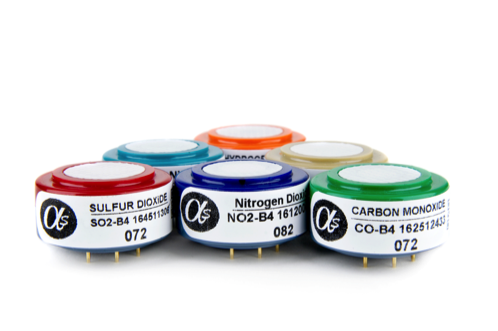
\includegraphics[width=\textwidth]{visuals/as_gas}               
 	 \caption{AlphaSense Electrochemical Gas Sensors.}
  	\label{fig:as_gas}
\end{marginfigure}

For sensing specific gases, many types of sensors are used.  Among other techniques, spectroscopy, chromatography, and chemiluminescence are very common for professional applications.  For mobile use, Alphasense sensors have emerged with a strong cost to performance ratio.  Alphasense sells Photoionization Detection based sensors, which work by ionizing gas particles with UV light and sensing the generated current over a fixed voltage in contact with the air. They also sell Nondispersive IR sensors, a simple optical absorption method.  

For the specific types of gases we're interested in, electrochemical techniques are the primary low cost method on the market.  The AlphaSense version is well-regarded, with ppb sensitivities and a clear failure condition (instead of the gradual drift you might expect as the sensor is depleted and dirtied). Electrochemical gas sensors are comprised of a working electrode, a reference electrode, and a counter electrode, all bathed in an electrolyte.  The reference electrode is used to control the voltage at the working electrode, and keep it in a linear current/voltage regime.  The working and counter electrodes promote inverse oxidation/reduction reactions, combining with the gas to produce free electrons, and then balancing that first reaction so as not to deplete or change the available reactants. The resulting current is proportional to the gas concentration, as long as corrections are applied for temperature, humidity, and pressure (and adequate time is allowed for 'warming up' once the reference electrode is powered on due to large inter-electrode capacitance).  These sensors are generally well-characterized under stable operating conditions, and have well understood cross-sensitivities and time-constants associated with their behavior.

While AlphaSense sensors can be purchased with calibration data, environmental sensing researchers at MIT have suggested that these calibrations are generally not accurate, and typically co-locate the sensors with a Federal Reference sensor for more rigorous calibration before deploying them elsewhere. 

\subsection{Measurement Strategies and Complications}

Historically, the standard measure of air quality has been a sparse network of fixed stations run by government agencies.  These extremely expensive and extremely large stations require manual calibration every few weeks.
	
While these stations are highly accurate, studies have shown they either chronically underreport or have no correlation with the personal exposure of the citizens living near them. Only with sophisticated modeling of elevation, geography, ambient conditions, wind velocity, and land use can these data be tied to exposure elsewhere in a city, and these models must be evaluated on a case-by-case and pollutant-by-pollutant basis.  
	
New techniques to map and model a city using a small number of medium quality, mobile sensors have started to emerge. Stationary, high quality sensors play an important role in calibrating these systems on-the-fly, but these methods have shown much better predictive power for mapping cities in higher spatial resolutions.  However, their predictive power is still best on timescales of years and weeks, and starts to break down as they move towards days and hours.

Models on these timescales and resolutions are useful for understanding general trends in exposure for a city, as well as identifying and eliminating pollution sources, hotspots of high exposure, and issues with urban planning.  However, even these mobile techniques for map generation are limited in their ability to predict personal exposure.

Personal exposure is so difficult to measure because pollutant concentrations can vary dynamically.  For certain conditions researchers have modeled this complex behavior, and thanks to expensive portable sensors there have been several studies to corroborate their findings.  One common phenomenon is called the 'urban canyon'-- a street with two tall buildings on either side that creates several interacting, swirling vortices.

Measurements have shown CO and UFP concentrations doubling on one side of the street relative to the other in an urban canyon, measured at the same time of day. This variability has been demonstrated time and again-- one study showed complex relationships between different pollutants measured in the center of the street versus the sidewalk. Different corners of the same intersection can also vary tremendously. Even walking roadside vs. building-side on the same sidewalk has been linked to significant differences in pollution exposure level.

This is all to say that spatial variation is extremely high.  Concentrations can change drastically over just a few meters.  For true personal exposure monitoring, it is regarded as best practice to sample air within 30cm of the mouth and nose. While some of these spatial phenomena may fit an urban canyon model, and some may be modeled accurately with standard dispersion, few real-world scenarios are predictable with any single technique (especially to within a few meters).  It is extremely difficult to predict real spatial variation without direct measurement. 

Temporal variation is equally difficult to monitor. Studies at traffic intersections have shown that regular, tenfold increases in pollutant concentration occur over just one second. This staggering variation is averaged out even with the some of the best 'real-time' techniques-- fifteen second integration would miss the entire event.  Peak exposure levels may have important health implications, and in most cases transient events like this account for the majority of urban exposure.

Given the tremendous spatiotemporal variation in pollution, wearable air quality monitoring is clearly the only viable path to accurate personal exposure data.  Fixed and mobile sensors, even with state-of-the-art predictive resolution, can't capture the detail required to estimate individual exposure (especially considering the accepted standard of 30 cm from the mouth and nose for accuracy). 

With enough adoption, it is not difficult to image improving the collection and prediction of city-wide pollution mapping traditionally associated with fixed sensor installations.  Eventually, wearable sensor data may even enable accurate path-based personal exposure modeling (statistical relevance on the order of meters and minutes), since the data is collected from varied users in the real microenvironments that dominate their exposure.  Accounting for this otherwise highly specific spatiotemporal resolution would be difficult with any alternative method (day and 100m2 resolution is the best we see with predictive models right now).  As mobile sensing increases in accuracy and drops in cost, distributed sensing will usher in a new way of understanding the pollution landscape and our exposure to it.


\section{Sensor Networks}

\subsection{Air Quality Sensor Networks}

It is not uncommon to see publications describing cheap and portable smart-phone based air quality projects.  In most cases, these publications focus on system design, and produce thought-provoking work on the user-interface.  In cases where technologists explore new sensor design, it is rare they achieve compelling improvements.  The past 20 year has seen a lot of incremental optimization in the most promising sensing modalities.  Few research labs are positioned to push the state-of-the-art further by simply re-applying the same core physics without a fundamentally new insight.  Significant effort has brought us to current level of sophistication, and any incremental progress at the sensor level requires an equally sophisticated understanding.   

Outside of phone applications, true system-level research in the air quality space is uncommon.  Most air quality networks use the same topology-- one type of sensor device with standard, centralized data collection methods.  The exception to this rule comes out of ETH Zurich's OpenSense project, where mobile sensors check their calibration as they pass higher-quality fixed sensors.  OpenSense has also pioneered methods for multi-hop mobile sensor calibration.  Their work sets the standard for exploratory new air quality sensor network topologies.

In the consumer space, many projects and devices are launching on regular basis.  Unfortunately, most devices do not stand up to independent scrutiny, and rarely do they offer meaningful improvements over the status quo.  None of these devices has succeeded at sustaining momentum.  SmartCitizen is an example-- after a successful 2014 kickstarter with 600 backers and \$68k raised, the SmartCitizen online network currently shows no active devices (despite 618 having been registered).  The constant barrage of 'new' monitoring devices-- without accountability, without rigorous data-collection, and without real-world use-cases-- saturates and dilutes consumer response to these important issues.   

Citizens aren't the only ones purchasing air quality sensor devices.  Many cities are installing high-density pollution monitoring networks-- in some cases, only later realizing that the data is not of reasonable quality.  London (quite publicly) recently released a network of GPS-tracked, tweeting pidgeons with NO2 sensor backpacks-- while driven by a marketing firm as a (very successful) publicity campaign, it is a safe bet that data quality assurance is low.

The EPA publicly states that distributed, cheap sensing technology will be a cornerstone of their future success.  As part of the effort to engage with active citizens and communities, the EPA measures and publishes data about low cost consumer devices.  Currently this is done by co-locating the consumer device with a Federal Reference Measurement (FRM) device outside for several months (usually through a change of seasons).  This validation is not standardized or rigorously defined.  The end result is a simple regression comparison (produced by hand), and a single designation for the sensor (i.e. 'good' or 'bad').  Other organizations do similar co-location experiments (like SCAQMD), but no standard procedure has been agreed upon.

\subsection{Large Scale Data Sharing}

The air quality research community is actively looking for solutions to facilitate inter-organization data-sharing, so that large scale collaboration can become more commonplace.  They are also actively working to educate, involve, and benefit from the citizen sensing movement.  There are many open questions around how to structure an ecosystem with variable quality data, how to define data standards, and how data should be hosted. 
 
The most common solution for large-scale data sharing is to construct a centralized 'cloud' database with strict data standards and a strict ontology.  Generally, users prepare their data to meet the standard, and then push their data to the database using some basic tools.  As the most common structure, there are options that have library support for various file formats and hardware platforms.  Examples include data.sparkfun.com (which integrates directly with arduino shields) or plenar.io (which has easy csv upload and nice data selection/access features).  

\subsection{ChainAPI}

When it comes to robust solutions for large scale sensor networks that directly feed into a database, the possible options are less well-defined.  An ideal ecosystem would allow large scale networks to interact seamlessly, while still allowing freedom in ontology and distributed hosting (similar to the World Wide Web).  While there are several solutions starting to appear for Internet of Things applications (the so called 'Web of Things'), many are over-specified, and up until now the practical result has been for industry players to silo their hardware, their data, and their applications.  Industry consortia are starting to form to address these problems,  but the issues are still unresolved.

ChainAPI offers a thin, HAL- and JSON-based hypermedia solution for creating a distributed, browsable data resource.  It dictates enough structure to make resources easily linkable, new ontological relationships easily definable, and datasets easily accessible, searchable, and streamable.  It leaves open the questions of ontology and backend database structure. 

ChainAPI has been successfully used for a large-scale ecological installation in Southern Massachussetts.  It serves as the backbone for many interesting data visualizations, audio compositions, and future-looking tools.  It provides extensible answers to many questions facing the world of large scale, distributed sensor installations and their associated data.

\subsection{Machine Learning}

Machine learning provides a way to design algorithms that learn and improve as more data is provided.  These techniques have been applied to sensor data in a variety of forms.  Examples range from predicting the number of people in a closed space by looking at changes in distributed sensor readings (i.e. temperature, humidity, light, and pressure), to predicting soil moisture based on remote sensing techniques (i.e. vegetation index and light backscatter).  One notable research project used HVAC sensor data, both analytically and redundantly, to predict and verify whether other sensors in the network were working properly and automatically replace unreliable data.

Generally, all of these examples use supervised learning approaches with some form of cross-validation to validate success.  While each uses a different core algorithm (and there is room to test and apply all of them to the air quality space), one worth mentioning is the logistic regression.  Logistic regression is frequently used to predict engineering failure of products or systems.  It can be applied as a binary classifier (i.e., 'Is this sensor failing?'), as well as give a probability for each outcome ('yes' or 'no').
  

\section{Motivation}

Air pollution is a health risk for people around the world.  While standard measurement techniques are highly accurate, they are also extremely expensive and stationary.  These stationary sensors fall short of capturing meaningful information about a citizen's personal exposure-- the spatiotemporal variations of pollution concentration are too complex and too narrowly resolved to be captured with a single, distant sensor.

For exacting personal monitoring, wearable, mobile sensing is the only answer.  Sensors do exist that can measure personal exposure, but they are either thousands of dollars or they are cheap and inaccurate.  While elusive, portable, affordable sensing, has the potential to offer powerful insights for both individuals and research organizations.

The lack of cheap solutions is not due to a lack of understanding.  The core device physics of most sensors have been well-optimized over several decades, and the sophistication underlying their reference level counterparts is truly remarkable.  Cheap sensors are starting to mirror the core principles of instrument-grade devices.  Unforunately, there are systemic failures in cheap systems that simply are fundamental to the underlying sensor modality.  

Optical sensors, for instance, require precision optics, heated inlets, flow control, and size-selective filtration.  Solutions to these problems require extra power, extra size, or extra cost (and frequently all three).  Addressing these problems would push a cheap, portable sensor out of its category.  Electrochemical gas sensors require a clean, precision doping process, a statistically minimal exposed surface area, and compensation for fow rate, pressure, temperature, humidity, and electrical noise.  The physics limit how small they can be, and the market limits how much cost can be driven out of the manufacturing process.

There are two main take-aways from this survey-- the first is that attempting to incrementally improve devices by re-exploring their core physics is a difficult proposition.  The core physics are well-understood and companies have been optimizing them successfully for decades.  The first order problems with cheap sensors are \textit{not} with the core device principles, but with well-understood failure modes (like flow control, fog, temperature dependence, or chemical cross-sensitivity).  

The second take-away is that, excitingly, the core physics underlying cheap commercial sensors are approaching a very high quality.  This suggests that the sensors-- when they fail to provide accurate readings-- are likely doing so because of systemic, predictable failures.  If that was one single failure (like an optical sensor that is reliable except when fog is present), it would be trivial to predict when the sensor data is reliable based on fog measurements.  In real-world scenarios, however, multiple failure modes compound and obfuscate underlying robustness.

The belief that cheap sensors are now entering a quality regime where failure is more predictable leads us to machine learning as a potentially powerful mechanism to explore sensor performance and improve reliability.  Machine learning is perfectly suited to tease out these complicated underlying relationships.  Instead of the common approach of \textit{improving} sensor performance, the research suggests that \textit{characterizing} and \textit{predicting} sensor reliability in a nuanced way is novel, necessary, and potentially revolutionary.

In many cases, first-order predictions may work well to predict sensor accuracy.  Gas sensors break in known ways and are specified for known operating ranges.  Simply monitoring its temperature/humidity/pressure exposure, its air-flow, and gas sensors of cross-sensitive pollutants could provide incredible insight.  

Second order insights are perhaps more interesting.  For instance, the OPC-N2 particle counter is likely to be confounded by road dust or pollen.  What if we could loosely approximate road dust exposure based on the user's location relative to a road, traffic patterns, the time of day, and the wind?  What if we could predict O3 measurement reliability based on the underlying drivers-- NO2, sunlight, and cloud cover? In this thesis, we explore both first-order and second-order insights using machine learning techniques.

Simple machine learning analysis could also provide an objective measure of sensor quality.  How well machine learning can predict a sensor's behavior is a nuanced way to measure its repeatability.  Sensors that fail spuriously instead of predictably are inferior in design and construction.  
     
For any of this to work, we need to compare our cheap sensor against a high quality reference, so we can learn when a sensor is in error, and what conditions may be indicitive of that error.  There is precedent for air quality network infrastructure that compares cheaper mobile sensors with a higher quality reference, but until now this has only been done as a basic calibration step.  This is the first predictive air quality system. 

In order to build such a system, we require a backend solution that can automatically compare EPA data to a cheaper network installation.  ChainAPI is well suited for this task, and in the process of building this infrastructure, we examine and address some of the biggest issues facing air quality data sharing, ecosystem building, and data interaction.  We also create an infrastructure that may be used to automatically measure and characterize consumer device quality, in a very nuanced, climate- and geography- specific way.

Finally, we believe such a system has the ability to contribute to and provoke a more nuanced, informed dialog in the citizen sensing community.  We propose the first device designed with the premise that its data \textit{won't be reliable}, that we need to predict when it is.  Inherent in the design is the suggestion that the a sensor's success is complex, based on a variety of factors.  This provocation could help inform and educate new users-- cutting through noise instead of adding to it.

There are many interesting problems currently facing the air quality community.  We believe a machine learning approach to predicting sensor accuracy could improve the reliabilty of cheap sensors, pushing the state-of-the-art forward.   Validating this data would opening up a world of reliable, distributed data to the research community.  In the process of testing this approach, we are building scalable solutions for data sharing and network interaction between cheap and expensive sensors.  We are also engaging the communitiy with a new perspective on how to approach affordable sensing.   


%http://vista.cira.colostate.edu/improve/publications/graylit/014_AerosolByNeph/AerosolbyNeph.pdf -lognormal distribution

%https://www.researchgate.net/publication/222076545_Estimating_Soil_Moisture_Using_Remote_Sensing_Data_A_Machine_Learning_Approach
%http://web.eecs.utk.edu/~new/publications/2013_ICMLA_SensorQualityML.pdf
%file:///Users/davidramsay/Downloads/CIT1913.pdf

%http://www.paulaoki.com/papers/sensys09-demo.pdf   'common-sense' cheap phone smog, phone based
%https://www.semanticscholar.org/paper/AirCloud-a-cloud-based-air-quality-monitoring-Cheng-Li/01d743e5c85cd68734ec148cbf485b59649c29dd 'aircloud' DIY PM sensing, nice app, push to cloud
%http://ieeexplore.ieee.org/stamp/stamp.jsp?arnumber=6758498  Haze watch sydney, spatial cars, phones to upload.

%http://www.tik.ee.ethz.ch/~saukho/paper/hasenfratz12participatory.pdf  ETH gas sense phone paper, route tracing, air flow issues discussed, O3 which tends to be a more stable pollutant as not a direct combustion by-product.

%something to look into
%http://citeseerx.ist.psu.edu/viewdoc/download?doi=10.1.1.714.3011&rep=rep1&type=pdf
\chapter{3. Related Work}

In this section we consider past air quality work in the context of mobile or personal sensing.  Additionally, we explore several of the cutting edge solutions for storing, manipulating, and displaying data of this type.

\section{Air Quality}

\subsection{Safecast}

Safecast \cite{safecast} is an organization created in response to the Fukushima disaster to crowd-source radiation measurements using open-source GPS-tracked geiger counters.  They have succeeded at creating and publishing the most detailed radiation maps in the world, and are now looking to apply their expertise to air quality.

We are already closely linked with the Safecast team, which has been working on open data and open hardware air quality sensing for about a year.  They've just finished an alpha version of a stationary air quality monitor.

\subsection{Aclima/Google}

Aclima \cite{aclima} is a San Francisco startup specializing in environmental sensor networks.  Last year, Google and Aclima started a mobile, car mounted air quality project.  However, their algorithms and hardware have not been shared and they appear to want to control all the data they generate.  The speculation is that they are using a quite expensive setup in the back of the car, slowly drawing in air over time.  

\subsection{Copenhagen Wheel Project}

Out of the MIT SENSEable lab, the Copenhagen wheel \cite{wheel} is mounted on a bike wheel to assist your pedaling, lock your bike, and capture data about air quality.  The original project was unveiled in 2009 and subsequently licensed to a Cambridge Area startup (Superpedestrian).  It is currently available for pre-order.  Air quality is a tertiary feature of their project, and no hardware specs or details about what they are planning to monitor have been released.

\subsection{OpenSense} 

An ETH based project, is the current world leader in mobile air quality sensor networks, with the first practical distributed mobile sensing platform using large devices mounted on the Zurich public tram system. \cite{hasen2011}  The OpenSense team has published many excellent articles that address some of the fundamental problems in low-cost, mobile air quality sensing.  They've laid the groundwork for dealing with gas sensor calibration (particularly with multi-hop calibration techniques), as well as advancing the state of the art in Land Use Regression modeling based on sparse, real-time, mobile, distributed measurement.  However, their resolution has only been tested up to 12 hour, 100m x 100m predictions (with accuracy much less than weekly/yearly predictions), and their sensors are large and run off of power from the trams they are mounted on. Their first attempt at truly personal sensing was a recent low-cost phone-enabled ozone sensor, which proved viable. \cite{hansen2012_2}  However, one of their assumptions for this device's success was that ozone has limited and predictable spatiotemporal variation (which is true, much less than other pollutants). Their preliminary tests with this sensor also revealed significant errors for high pollution levels when under airflow. \cite{hasen2014, hasen2012, saukh2015}
	
\subsection{TRUSS}

Similar to OpenSense, the TRUSS (Tracking Risk with Ubiquitous Smart Sensing) project from the Media Lab's Responsive Environments group similarly blends high-power, fixed sensors with low-power, wearable nodes to provide real-time sensor fusion and insight. \cite{truss}  In particular, this project examined and compared multiple air quality sensors to predict harmful conditions-- however, the goal of this work was to detect coarse, major risk instead of precise, ambient exposure.

\subsection{Cheap Sensor Development and Testing Groups}

There are organizations (such as South Coast Air Quality Management District [SCAQMD], the UK's National Physical Laboratory, and the EPA) that are testing and characterizing cheap optical PM sensors in real-world scenarios. There is also an active research community around developing MEMS PM sensors (using tech like FBAR, or Film Bulk Acoustic Resonators).  These groups are essential for independently testing the claims of new products, and provide important insight into the trends with respect to the success and failure of new sensor technology.

\subsection{Other}

There are many other projects that appear in the air quality space, each with some unique take on affordable, distributed air quality.  Most of the following projects are successful in one or more aspects of their system design, but do not innovate with their core sensor physics or algorithm. 

These projects include MIT's stationary/expensive Clarity sensing project, \cite{clarity} the independent and nicely designed tricorder sensor platform, \cite{tricorder} the innovative Propeller Health project that extrapolates pollution data from asthmatic inhaler usage, \cite{propeller} the open source and mobile UPOD project, \cite{upod} the mobile Italian uSense project, \cite{usense} the 'wearable' AirBeam kickstarter project, \cite{airbeam} the Boston based startup Elm that translates their distributed air quality data into useable advice (and has an open invitation on their site to hook your sensor into their network), \cite{elm} the Israeli BreezoMeter startup that extrapolates street-level/high resolution air quality data (presumably from wind patterns and known reference data), \cite{breeze} the London-based company cleanSpace that provides air quality maps and incentivizes air quality friendly commuting, \cite{cleanspace} the startups Clarity and Tzoa that are selling versions of the 'world's smallest' PM2.5 wearable, \cite{ clarity2, tzoa} and the startup uHoo which is building a home air quality monitor. \cite{uhoo}  Other slightly less interesting, but still notable, include a handful of other hardware/commercial projects (the Air Quality Egg, \cite{egg} CMU's Speck, \cite{speck} Atmotube, \cite{atmotube} AirboxLab, \cite{airbox} SmartCitizen \cite{sck}) and independent research like the French citizenAir project \cite{citizenair} and DIY Public Labs work. \cite{publiclabs}  New projects in this space appear on a regular basis. 

\section{Data Sharing Solutions}

There are many options for data-sharing, particularly when exploring options that have a centralized entrypoint.  Open source tools like Django \cite{django} allow system administrators to easily spin up their own database solutions and create front-end tools, while services like plenar.io offer simple, managed solutions for data upload, display, and download.  

An interesting open-source solution is Apache Hadoop, \cite{hadoop} which is a database backend that can handle distributed storage and distributed processing for very large datasets.  It can run on Amazon Web Services or Google Cloud, and has been used by many large companies.  While interesting, it is not designed for easy input/output of data, but instead for managing and parallelizing computation on large datasets using Java (where everything is done in the cloud).  This solution is likely over-technical and over-specified for the air quality use case.  


\subsection{The Semantic Web - RDF, HAL, and JSON-LD}

An alternative, simple, distributed solution comes in the form of the semantic web.  Instead of thinking of our data as separate from our devices-- where researchers must pull data by hand, process it, and then upload it to a repository-- it makes more sense to take an 'Internet of Things' approach.  The advantages of this system are many-- it provides transparency to the measurement technique (data is associated with the device, and metadata about the device, that uploaded it) as well as to the processing steps (data is uploaded in a raw form, and processed in the web).  It also provides an intuitive, physical hierarchy for organizing and linking device and sensor data resources together.  With proper system design, the researcher should not have to manually upload anything-- they should be able to automatically pull all of the latest data (including automatically calibrated/processed data) from the database without ever manually pushing it there in the first place.

This type of sensor network design is not new.  Most large sensor network installations automatically push their data up to a central server.  By adding a semantic web layer on top of these servers, it is simple to connect devices and sensors in a much larger 'Web of Things'.  Many standards for achieving this have been proposed over recent years.    

Resource Description Format (RDF) is one of the most noteworthy foundations in semantic web thinking. \cite{RDF}  It represents a data model specification-- every web resource (for instance, a device or a sensor object stored at a given URI)-- has defined relationships through 'triples' of the form subject-predicate-object.  An example would be 'device #1 includes sensor #5', which would be represented with URIs (http://device/1, http://relation/includes, http://sensor/5).  This creates a labeled, directed multi-graph data model.  It has been adapted to many standards and syntaxes like XML, and extended in standards like OWL (Web Ontology Language) or Turtle (Terse RDF Triple Language).  The syntactic extension of this format in JSON -- the current lingua franca of web data-- is known as JSON-LD, and has been advocated for by Tim Berners-Lee (inventor of the World Wide Web). \cite{jsonld}

HAL, or Hypertext Application Language, is another hypermedia semantic web data model with XML and JSON formats. \cite{hal}  It similarly defines relations to other resources using a shared URI, so ontologies can be easily added and extended.  It is simpler than JSON-LD, with each resource limited to its attributes and its external link relations.  HAL supports simple embedded resources and URI prefixing.


\subsection{IoTivity and AllJoyn}

Industry consortia are starting to take steps to build their own 'Web of Things' using the internet backbone.  The two largest are IoTivity-- a project by the Linux Foundation and Samsung-- and Qualcomm's AllJoyn. \cite{iot, alljoyn}  They support low level protocols like CoAP, large APIs for interfacing with connected devices, and end-to-end device discovery and connection solutions.  While these tools may gain prominence over the next several years, for now they are in their infancy, and looking to address more fundamental infrastructure/connectivity problems (focusing more on real-time queries and connectivity rather than data storage, management, and sharing).
		
\subsection{ChainAPI and TidMarsh}

ChainAPI \cite{chainGit, chainPaper} is a standard for data sharing based on HAL and JSON developed in the Responsive Environments group at the MIT Media Lab.  It does not attempt to specify end-to-end connectivity, nor does it force any specific implementation or ontology-- it simply wraps the HAL semantic web specification with common-sense design principles to make interoperability and data access simple and intuitive.  This level of specificity enables a very low barrier to entry and very flexible use, while still providing enough structure to support a large, coherent ecosystem.

ChainAPI has been tested and used in the MIT Media Lab's TidMarsh project to store and expose ecological data from hundreds of local sensors over dozens of devices.  This implementation includes a browsable web front-end, and several forward looking applications that take advantage of ChainAPI's streamability-- a live, constantly updating virtual representation of the sensed environment is available at tidmarsh.media.mit.edu.  Electronic music compositions have been written that stream and use live data from the Marsh. \cite{evan}  Several elaborate data visualization scripts have also been written on top of ChainAPI. \cite{tidviz}

ChainAPI has a low barrier to entry, an extensible ontology, provides easy access to streamable data, and can quickly scale in a distributed manner.  It is as simple as possible without sacrificing functionality.
\chapter{4. Overview of Design and Contributions}

The are three main goals with the learnAir project.  The first of is (1) to evaluate the usefulness and feasibility of applying machine learning algorithms to air quality sensor networks.  Specifically, this means testing whether we can predict when a cheaper sensor is giving reliable data based on the conditions under which it is measuring. The second goal is (2) to prototype a data solution that addresses the needs of the air quality sensing community-- particularly, the creation of an ecosystem that supports the needs of participants from high-end research facilities to low-accuracy citizen projects-- and allows seamless, easy interaction between them.  It also must support scalable, automatic support for the machine learning algorithms validated as part of our first goal.  Finally, we want (3) to prototype an actual, handheld system that uses the algorithms from (1) and the database from (2) to realize a deployable, useful, provocative mobile sensor system that demonstrates the concepts and ideas put forth in this thesis.  We believe this device will serve as a powerful rhetorical tool and push the dialog forward in citizen sensing communities.  We also believe this system will give improved data reliability and a more accurate picture of personal exposure compared to comparably priced and speced systems.      

The final system will enable a sensor to learn about itself when it is near a higher quality reference.  It will apply that knowledge to new measurements made under new conditions, even as it moves away from the reference system.  Every measurement the system makes will be accompanied by a simple prediction-- was this measurement accurate or not?  Every prediction will also come with an estimate of certainty-- how confident are we this prediction is accurate?  As more sensors of the same make and model are added to the network, new predictions will improve and older predictions will be revised.

\section{Machine Learning Validation}

Sensor technology-- especially in the air quality space-- is getting cheaper and more reliable.  For the first time, well-reputed sensors are starting to appear in the \$100 range.  However, there are limitations on what is possible with small, cheap technology.  For example, electrochemical gas sensors break down in known ways-- their reactions are temperature, pressure, and humidity dependent, in some cases they are cross-sensitive to other gases, and their reactions have time-constants and noise suceptibility based on electrode size and exposure area.  Optical particulate sensors are frequently designed to mitigate external effects by applying (expensive) precise air flow control, heated inlets to eliminate fog, size-selective particle filtering, and advanced optics.

Sensors that break down in systemic ways may provide very reliable information under certain conditions.  While it may be obvious if a sensor has one, very clear failure mode (for instance, an optical sensor that is very reliable unless there is fog), compounded failure modes are more common and more difficult to infer.  By applying machine learning to this problem, we can automatically characterize which and how strongly underlying features are predictive of systematic errors.  

Machine learning has a strong likelihood for providing insight into sensor reliability assuming the sensors are not spurious-- that there failures come predictably.  This assumption has likely not been true in the past, but the evidence suggests that we've entered into a new era of cheap air quality sensing-- where some devices implement trustworthy, strong designs, but simply cannot afford to build a controlled environment around the measurement sample typical for instrument level devices.  In these cases, we can measure the conditions instead of controlling them, and make an educated prediction about the reliability of our measurement.      

To put this theory to the test, we built a stationary device that can measure ambient conditions (temperature, light, humidity, wind) with a range of cheap air quality sensors for CO, NO2, O3, and particulate.  This sensor is called 'learnAir V1'.  This sensor was installed for ~2 months at a Mass Department of Environmental Protection (MassDEP) measurement site, right next to the inlet for expensive, reference EPA measurement equipment.  The data collected from our measurements was used to compare against the 'ground truth' provided by the EPA, to characterize when the sensors were reading accurately and when they weren't.  We then used machine learning techniques to predict when the sensor was giving accurate readings or not. Using cross-validation techniques (splitting our collected data into a training set and a testing set), we can characterize how well our algorithms predict our sensors accuracy.  See Chapter 5 for a description of the device and MassDEP reference hardware, and Chapter 7 for an in-depth analysis of the machine learning techniques and cross-validation results.      
 
\section{ChainAPI Instance and Tools}

The air quality research community is actively working to mitigate the complications involved with inter-organization data-sharing.  Furthermore, they are interested and actively engaged in questions around the citizen sensing movement-- how should they inform and involve citizens in the air quality monitoring community?  How should they validate cheap consumer devices?  Is there a research use for the lower-quality data gathered from these networks, and how can they access and interact with it? 

Another contribution of this thesis is to build and adapt an instance of ChainAPI-- a hypermedia data-sharing framework-- for use with air quality data.  ChainAPI offers many interesting advantages for sensor deployments as a thin, distributed hypermedia layer for linking data resources.  It provides unique advantages for a diverse, distributed ecosystem where different sub-communities can co-exist.  

In addition to creating a new ontology for air quality resources and building a development ChainAPI server, several new tools are necessary to interact with the ChainAPI air quality ecosystem.  The infrastructure built for this thesis provides automatic resource discovery and dataset creation-- so researchers can automatically find and interact with new datasets based on the type of data they are interested in working with, without a priori knowledge of where to look for that data.  Its tools provides seperation of concerns, so that raw data and data processing scripts are seperated, instead of pre-processing occuring in an opaque way before data upload.  Its processing scripts-- that crawl through ChainAPI and update data-- offer transparency to data quality and data manipulation.  

This topology allows experts with certain sensors or devices to create, own, and update the processing elements for their technologies, and provide automatic, high-quality processing to novice users.  It provides the opportunity to create scripts that crawl through datasets looking for anomolies, out-of-spec operating characteristics, or out-of-service parts, and warn the device owners or data users.  Finally, it offers the ability to create learning algorithms that automatically improve as more data is added to the ChainAPI ecosystem. 

This contribution is a powerful example of how ChainAPI could be adapted for air quality data sharing.  It includes a new ontology based on the needs of the air quality community, and a large suite of tools that make ChainAPI a scalable, powerful tool for dynamic, growing ecosystems.  It also forms the basis for a truly automatic implementation of our machine learning algorithms.  See Chapter 6 for an in depth discussion of the contributions around ChainAPI.

\section{A Provocative Example}

Based on the infrastructure developed with ChainAPI and the algorithms tested at the EPA site, the final goal of the project is to build a fully functional, portable device that integrates all of these features.  There are several motivations for this: (1) as a rhetorical tool, to engage the citizen sensing community in a dialog about sensor data quality and validation, (2) as a means for deploying successful results from the previous sections as a best-in-class, trustworthy, manufacturable device, and (3) as a tool and platform for future testing of mobile use cases without having to do extensive data processing and manipulation by hand.  Once this system is built, the machine learning results and comparisons can be generated easily and automatically as long as the data is available in the ChainAPI ecosystem.

Two portable prototypes were designed and built as part of this thesis-- called 'learnAir V2' and 'learnAir V3'.  Both are battery powered, hand-held devices that integrate AlphaSense electrochemical and particulate sensors.  Both connect to a smartphone over BLE and push their data up to ChainAPI using GPS data from the phone application.  Both monitor ambient conditions of their measurements (vibration, temperature, humidity, light, wind) to help predict their accuracy.  

The two versions are very similar-- the main difference is the core microcontroller.  Version 2 is based on the Atmel ATmega32u4, and was programmed using the Arduino environment.  Version 3 is based on the lower-power, fully-featured STMicro STM32L152, and requires a more complicated build process, and comes with less library support.  There are cost and power savings associated with Version 3 (making it more 'production-worthy'), but functionally they are nearly identical solutions.  See Chapter 5 for an in-depth discussion of this hardware.



















%here's text referencing the (Table \ref{tab:sample_table}).
%
%\begin{table}
%  \centering
%  \begin{tabular}{l l l l l}
%    Column A & Column B & Column C & Column D & Column E \\
%    \toprule
%    A & B & C & D & E
%  \end{tabular}
%  \caption{A meaningless table}
%  \label{tab:sample_table}
%\end{table}

%Here's text referencing the margin figure (Figure \ref{fig:spin_margin}).
%
%\marginnote{\textbf{Margin Note:} Check it out, here's a margin note.}
%
%\begin{marginfigure}[{-10cm}]
% 	\includegraphics[width=\textwidth]{chap1/spin}               
% 	 \caption{Check it out, it's a Spin margin figure \url{spin.media.mit.edu}}
%  	\label{fig:spin_margin}
%\end{marginfigure}

%\begin{figure}[htb]
% 	\includegraphics[width=\textwidth]{chap1/spin}               
% 	 \caption{Check it out, it's a Spin \url{spin.media.mit.edu}}
%  	\label{fig:spin}
%\end{figure}
\chapter{5. Hardware Design and Analysis}

The vision of learnAir is to create a high-quality, affordable, and portable air quality monitor that (1) measures several pollutants, (2) measures ambient conditions like temperature, humidity, and light level, and (3) connects to a smartphone application that can display results, can send timestamp and geotagged data to the cloud, and can receive and display a prediction of measurement certainy based on machine learning applied to the data in the cloud.

Three learnAir devices have been built and tested.  The first (learnAir V1) is not portable, internet-connected, or battery powered-- it was solely used to collect sensor data that could be compared against higher quality MassDEP data for testing the feasibility and usefulness of predictive machine learning techniques.  This device was installed on a MassDEP (Department of Environmental Protection) monitoring site for 59 days-- from April 15th to June 13th 2016.

The second and third devices were designed to take the information gleaned from learnAir V1 and put it in a cheap, portable, smart-phone connected package.  The main circuit boards for LearnAir V2 and V3 were designed to match the size of the AlphaSense Analog Front End conditioning board-- a reasonably priced production board with three electrochemical gas sensors that has gained a strong reputation in the pollution sensing community.  These boards are BLE-enabled, and connect to two custom daughter boards for monitoring temperature, humidity, light level, UV exposure, and 3-axis wind speed.   

The two boards share power circuitry and most peripherals-- their central distinction is the main microcontroller.  LearnAir V2 is a fully functioning board based on the Atmel ATmega32u4, which requires an external RTC (real-time clock).  Firmware was written using a modified version of the Arduino codebase.  The third version is based on the STM32L152-- a more sophisticated, production-level microprocessor, with more optimization for low-power states, more SD card read/write support features, and an onboard RTC.  This third revision was also designed with a significantly smaller, soon-to-be available MEMS pressure sensor, which could reduce the volume occupied by the wind sensing module 50-fold (a large space savings from the current, large volume of 20mm x 60mm x 22mm).
     
The boards connect to a cross-platform smartphone application written in Javascript using Phonegap, a library that will compile javascript as webviews into iOS and Andriod applications.  It has plugins to access the phone GPS, and a simple D3.js library was used for plotting.  ChainAPI- our backend solution- supports  websocket connections and a subscription model to push data to the cloud and receive the latest predictions.



\section{LearnAir Version 1}
\FloatBarrier

LearnAir V1 was created to collect data with a variety of cheaper air quality sensors at a MassDEP monitoring site, to test our ability to predict a sensor's accuracy with machine learning by comparing it to a high quality reference.  The final box is 200mm x 120mm x 75mm (~ 8 x 5 x 3in), and houses two main subsystems.

\begin{marginfigure}
 	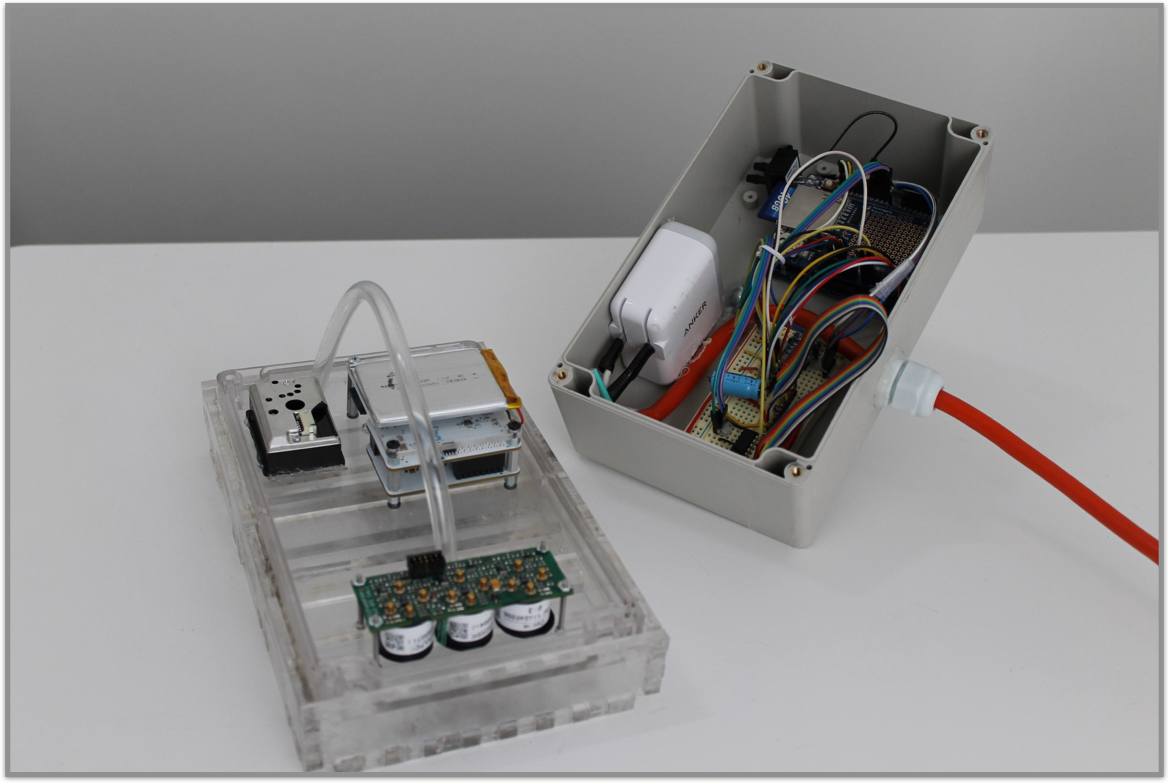
\includegraphics[width=\textwidth]{visuals/learnairV1}               
 	 \caption{LearnAir Sensor installed at MassDEP site, opened}
  	\label{fig:learnairv1}
\end{marginfigure}

\begin{figure}[htb]
 	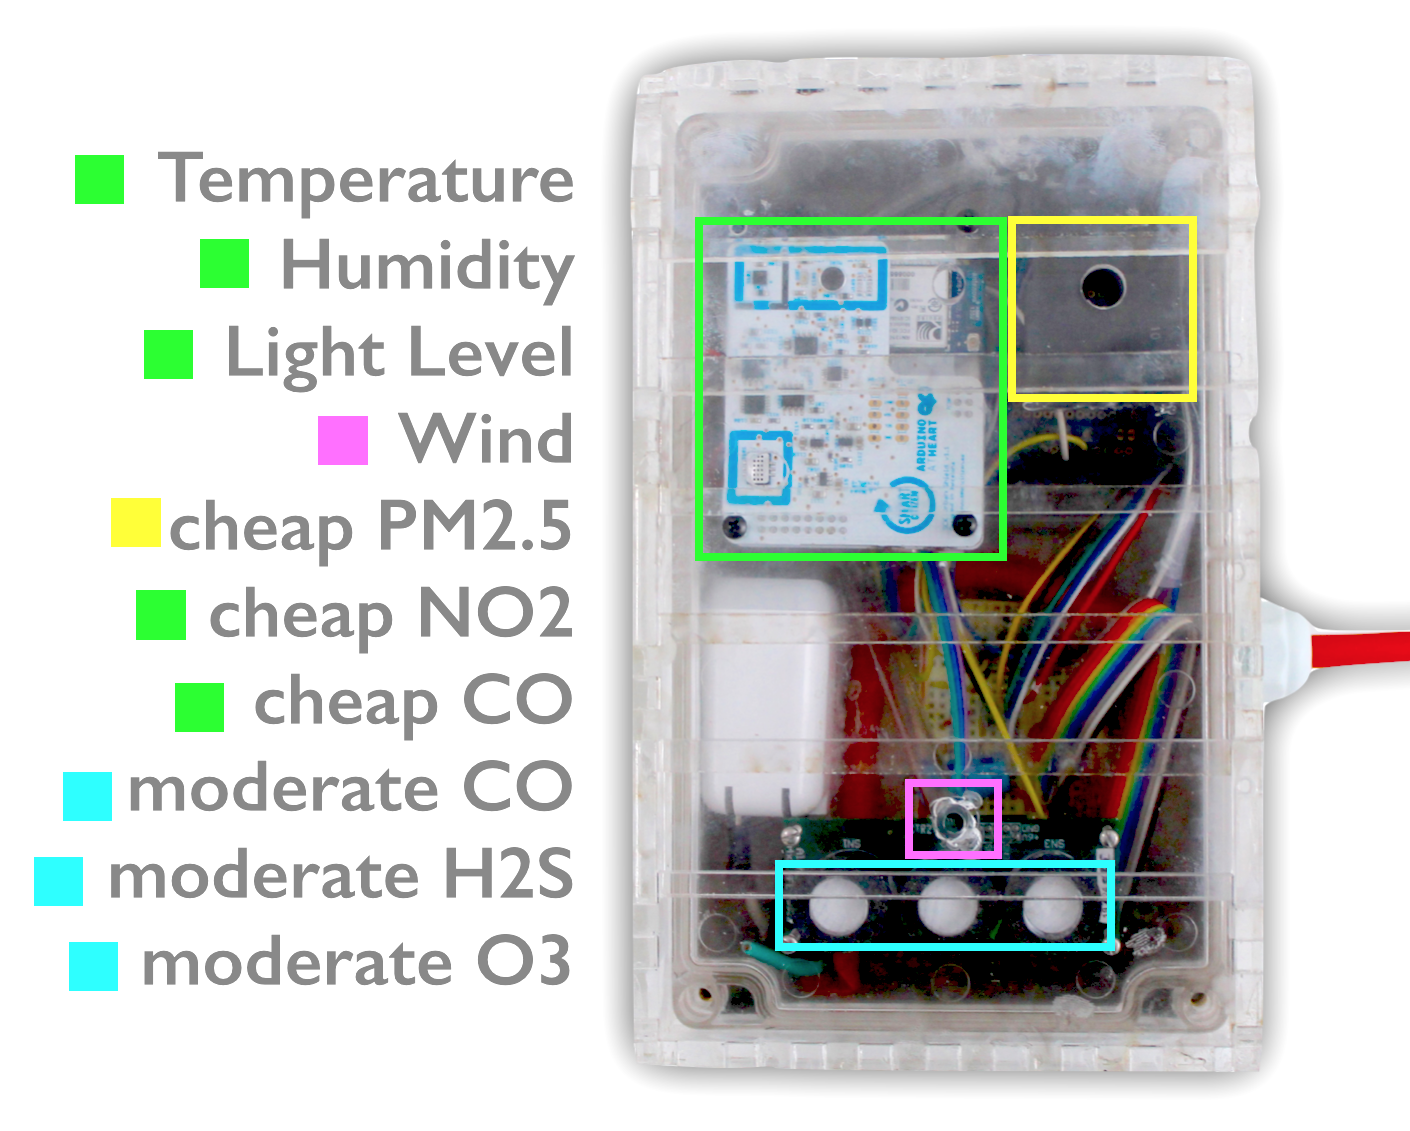
\includegraphics[width=\textwidth]{visuals/learnairV1_labeled}               
 	 \caption{LearnAir Sensor installed at MassDEP site}
  	\label{fig:learnairv1_labeled}
\end{figure}

The first sub-system is an off-the-shelf air quality monitoring system called the SmartCitizen Kit (frequently abbreviated SCK). \cite{sck}  The SmartCitizen Kit is Arduino-based (using the ATmega32u4), so custom code can easily be written and applied to the hardware.  This system was used in an offline data-logging mode, with raw data streams stored to the onboard micro-SD card for later retrieval.  

The SmartCitizen Kit includes several important sensors for our machine learning test.  It has a \textbf{DS1307} real-time clock for timestamping data and sample timing, a \textbf{MicroSD slot} for saving CSV files, a ROHM \textbf{BH1730FVC} I2C light sensor to monitor ambient light levels, a PUI \textbf{POM-3044P-R} electret microphone for monitoring ambient noise level, and a Sensirion \textbf{SHT21} I2C temperature and humidity sensor.  Most importantly, it has an E2V \textbf{MiCS-4514} CO and NO2 sensor.  This is a \$10, MEMS sensor-- one of the cheapest air quality sensors available.  It works on a Reduction/Oxidation principle, and has small internal heating elements.  It claims a 1-1000 ppm measurement range for CO and a 0.05-10ppm measurement range for NO2, and omits any information about reaction speed or cross-sensitivity in the datasheet.

The SmartCitizen Kit was mounted to the front of the case, with a small hole to expose the relevant sensors to the air.  Every hole in the case was gasketed with silicone, and the front of the case was mounted face down to minimize rain exposure.  Furthermore, a clear-acrylic, overlapping, slotted cover was designed to further protect the exposed sensing elements from rain and direct exposure.  

Despite the effort to protect the circuitry, the SmartCitizen Kit corroded severely in our first outdoor test.  A new kit was installed, this time with a layer of conformal coating added to prevent corrosion (Figure \ref{fig:sck_corroded}).  This addition prevented further corrosion for the remainder of the two month installation.    

\begin{marginfigure}
 	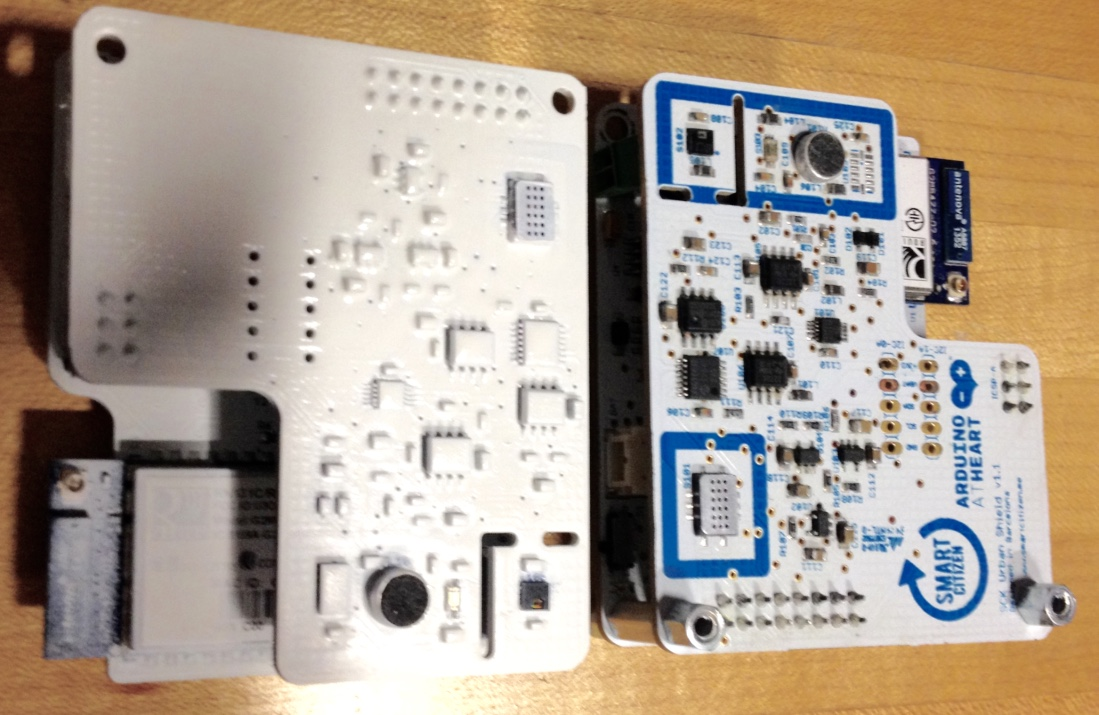
\includegraphics[width=\textwidth]{visuals/sck_conformal}               
 	 \caption{Corroded SmartCitizen Kit on the right, Conformal-coated new kit on the left.  Relevant sensors on the new kit were taped off before coating to prevent contamination}
  	\label{fig:sck_corroded}
\end{marginfigure}

Besides the SmartCitizen Kit, a custom Arduino-based sub-system is part of the platform.  This system is based on an Arduino Leonardo board (Atmel ATmega32u4) with an Adafruit data-logging shield (which includes an \textbf{SD card slot} and a Maxim \textbf{DS1307} RTC for timestamping-- the same RTC as the SmartCitizen). 

Three main sensor sub-systems were connected to this Arduino using a secondary prototyping board.  First, a \$10 Sharp \textbf{GP2Y1010AU0F} Optical Dust sensor was connected.  This sensor requires an external charging circuit to store energy for a narrow IR light pulse that is used to detect scattering.  These sensors have a reasonable reputation, and have shown good correlation with better quality sensors under controlled conditions indoors.  \cite{prabakar2015, austin2015} In real-world situations, they are unreliable.  

Secondly, an \textbf{AlphaSense Analog Front End Board} was connected.  This board supports three AlphaSense electrochemical gas sensors, which each have a Working and Auxiliary Electrode measurement.  Additionally, this board provides an onboard temperature measurement for sensor calibration.  All of these signals were multiplexed through an external TI \textbf{CD54HC4051e} multiplexer before connection to the Arduino 10-bit ADC.  Alphasense sensors are well-reputed, mid-level sensors-- they typically cost \$60-100 each, with the support circuit adding an additional \$150 in cost.  These sensors have t$_9_0$ response times of 10 ppm in ~20 seconds for CO, 1 ppm in ~30 seconds for NO2, and 100 ppb in ~15 seconds for O3.  Cross-sensitivity of the O3 sensors to NO2 is quite high (70-120\% measured with NO2 levels of 5ppm), as well as vice versa. (The NO2 sensor picks up 30-60\% of O3 at 100ppm.)  Other cross-sensitivities are well-documented and much smaller.  These sensors sport very low monitoring thresholds, well-characterized calibrations for electrolyte depletion and temperature dependence, and specified operating ranges for pressure, temperature, and humidity.

Finally, an Omron \textbf{D6F-PH} differential pressure sensor was included as a cheap, experimental way to measure airflow and wind.  This pressure sensor has two outlets- one was left vented into the box, and one was connected through a tube to the surface of the device.  Airflow over the top of the device creates a measurable pressure differential.  This sensor runs an I2C interface at 3.3V (which is incompatible with the 5V Arduino), so an external BSS138 level shifter from Adafruit was required to properly interface with the sensor.  All of these sensors were mounted to the front of the case, and gasketed to prevent unintended air exposure.

The final system is shown in Figures \ref{fig:learnairv1} and \ref{fig:learnairv1_labeled}.  An extension cord was spliced and soldered to a dual port USB charger, with powered both systems off of 5V USB.  This extension cord was inserted through a cable gland in the side of the box.  A metal mounting bracket extends from the back of the device.  Both sub-systems were configured to sample their sensors every 30 seconds.




\section{MassDEP Site}

Thanks to the generosity of the Massachusetts Department of Environmental Protection, I was given full access to their Roxbury Monitoring Site, allowed to co-locate the learnAir V1 sensor with their sensing inlet (approximately 3 feet away), and provided (normally unpublished) high time-resolution data.  The Roxbury monitoring site is the only one in the greater Boston area that has the capability to monitor particulate levels (through hourly Beta Attenuation Monitoring [BAM] measurements of black carbon), as well as minute-resolution data for trace gases (CO, NO, NO2, and O3).  We were also provided with high quality, minute-resolved windspeed and wind direction data, which we used to analyze our experimental differential pressure wind sensor and included as a training feature in our machine learning data.      

\begin{marginfigure}[3.5cm]
 	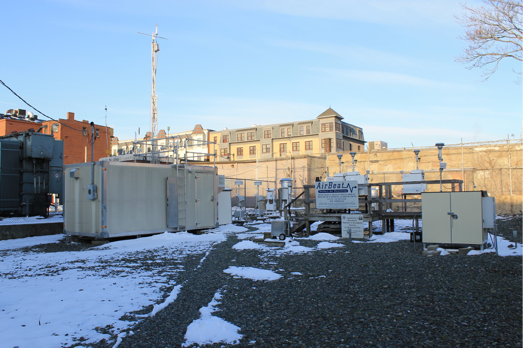
\includegraphics[width=\textwidth]{visuals/epa}               
 	 \caption{A picture of the Roxbury MassDEP measurement site where the LearnAir sensor was installed}
  	\label{fig:epa}
\end{marginfigure}

\begin{figure}[htb]
 	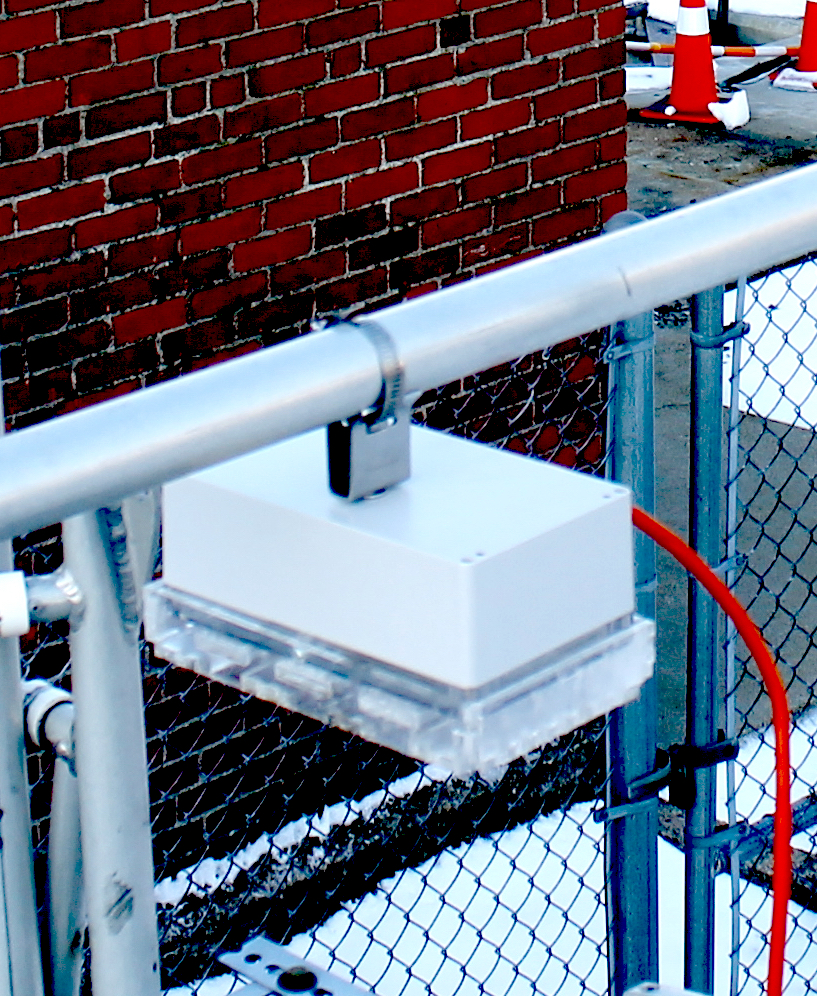
\includegraphics[width=\textwidth]{visuals/learnairV1_installed_zoomed}               
 	 \caption{LearnAir Sensor installed at the MassDEP site, close-up}
  	\label{fig:learnair_installed_zoomed}
\end{figure}

\begin{figure}[htb]
 	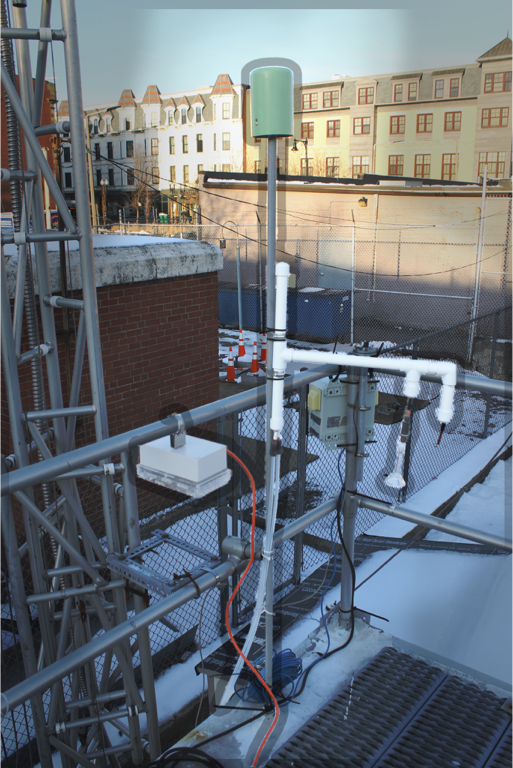
\includegraphics[width=\textwidth]{visuals/epa_zoom}               
 	 \caption{LearnAir Sensor (box on left) installation next to MassDEP inlet (top of pole on right)}
  	\label{fig:epa_zoom}
\end{figure}

The data provided by MassDEP is monitored weekly for quality assurance.  Each piece of sensor technology is in the \$10-100k range.  The EPA specifies Federal Reference Method (FRM) devices (devices that are accepted as the reliable standard for research use and to compare other devices against), as well as Federal Equivalence Method (FEM) devices, which may use other techniques but are acceptable replacements for FRM techniques.  All of these reference devices include FRM or FEM certification.

Black Carbon measurements were done with a Teledyne Model 633 Aethalometer sensor system which operates similar to the BAM style measurement.  This type of measurement draws air through filter paper for a period of time, and then irradiates it with UV and IR light to see how well the captured particulate attenuates it.  This means that-- though the measurement is incredibly robust and reliable-- the time-scale for measurements is on the order of an hour, and is an average of the accumulation over that period.  For the system we were using, a `10 a.m.' reading is exposed to air from 10:00 to 10:50 a.m., and measured between 10:50 and 11a.m., before the next reading begins.  Measurements are reported as \(\mu g/m^3\).
   
Wind speed and direction data was captured on a minute time-scale with a high-quality, vane style Met One 50.5H Sonic anemometer.  Trustworthy wind sensing data at these price points is non-controversial.  Measurements are reported in approach angle (degrees) for the direction and m/s for speed.

For gaseous pollution measurements, all of the reference equipment comes from Teledyne Advanced Pollutant Instruments.  The system is fed by an expensive, size-selective inlet with precise flow control.  Air is actively pulled through the system at a known, fixed rate.   Cross-sensitivity is not an issue for any of these devices.  

For NO and NO2 measurements, the Teledyne Model 200E Chemiluminescence Sensor is used. NO is measured by exposing the gas to O3 and measuring chemiluminescence, and a catalytic-reactive converter then converts NO2 to NO and repeats the measurement.  It has a precision of 0.5\% of its reading, and a t$_9_5$ of 60 seconds for its full operating range of 20 ppm, at a 0.5 L/min flow rate.  It is capable of reporting the average over a sample period or the instantaneous value.  It includes an adaptive filter that averages 42 samples over 5.6 minutes by default, unless it detects a rapid change in concentration (comparing an instantaneous reading to the long filter average), in which case it switches to a short-term, 6 sample, 48 second average.     

For O3 measurements, the FEM Model T400 UV Absorption system is used.  It has a 0.5 ppb sensitivity, and a t$_9_5$ of 20 seconds for its full operating range of 10ppm at a 800cc/min flow rate.  This system works on the Beer-Lambert law, alternately comparing the absorption of a stream the sampled air with an O3 filtered stream every 3 seconds using UV light (and correcting for temperature and pressure of the gas).  It is capable of reporting the average over a sample period or the instantaneous value. Its adaptive filter averages 32 samples over 96 seconds by default, switching to a short-term, 6 sample, 18 second average with rapid changes in concentration.

For CO, the FEM Model 300EU Gas Filter Correlation system is used.  It has a 0.5\% precision, and a t$_9_5$ of 30 seconds for its full operating range of 100ppm, at a 1.8 L/min flow rate  It similarly uses the Beer-Lambert law and IR light to compare a scrubbed sample with the untouched air.  It is also capable of reporting the average over a sample period or the instantaneous value.  Its adaptive filter averages 750 samples over 150 seconds by default, switching to a short-term, 48 sample, 10 second average with rapid changes in concentration.     

We installed the learnAir system face-down on the roof railing of the main air monitoring building, about three feet from the reference sensor inlet, as seen in Figure \ref{fig:epa_zoom}.  Our sensor and the inlet both face downward, however the Federal reference system has active airflow.  These inlets are mounted approximately 12 feet in the air and about 30-40 feet from the street.

\FloatBarrier
\begin{figure}[htb]
 	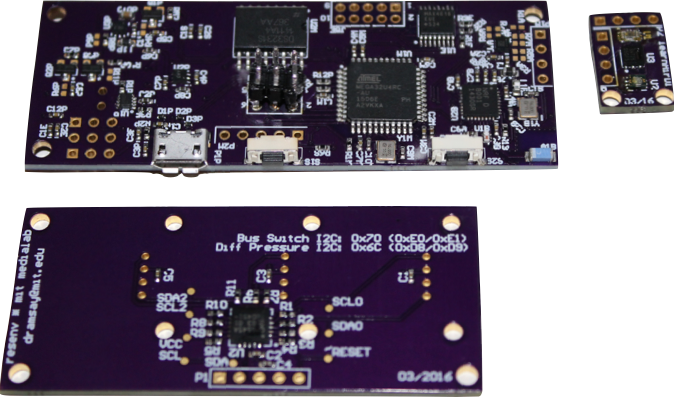
\includegraphics[width=\textwidth]{visuals/learnairV2_out}               
 	 \caption{Main and daughter boards of learnAir V2.0}
  	\label{fig:learnairv2_out}
\end{figure}
\FloatBarrier
\section{LearnAir Version 2}
\FloatBarrier

While the first hardware device we built was designed to collect data for testing and validation of learning algorithms, it does not represent a scalable, portable, cheap solution.  For that, we designed learnAir V2.

LearnAir V2 was created to be inexpensive, handheld, and portable.  It is designed to measure ambient conditions-- just like learnAir V1-- while still collecting the relevant air quality data.  It is battery-powered and smartphone connected, so that data can be seamlessly GPS-tagged, viewed in real-time, and sent to the cloud.  The outline of the internal circuit board was designed to mate with the AlphaSense AFE board.  AlphaSense sensors come well recommended in the air quality sensing community.  

The circuit design for LearnAir V2 is shown in Figure \ref{fig:learnairv2_out}.  It consists of a main board, designed around the Atmel ATmega32u4, and two daughter boards.  The main board sports a \textbf{micro-SD card} slot for storing data, a Nordic \textbf{nrf8001} with a chip antennae for Bluetooth Low Energy communication with a phone, a \textbf{microUSB} connector for charging the device and interacting with the microcontroller over USB, a ST \textbf{LIS2DH12} accelerometer to measure 3-axis motion and vibration, a TI \textbf{MAX4618} multiplexer to handle communication and mating to the AlphaSense frontend board, a Maxim \textbf{DS3231} RTC (from the same family as the DS1307 used in learnAir V1 but with temperature compensation and much more accurate timing), and standard breakout headers for several I2C and SPI environmental sensing peripherals at both 5V and 3.3V.  The main circuit is powered off of 3.3V to save on power, but 5V power handling is included.  Power to 5V peripherals can be programmatically shut on and off by the microcontroller for power saving when sleeping high quiesent devices.  Schematics for learnAir V2 can be found in Appendix B.

\begin{marginfigure}[3.5cm]
 	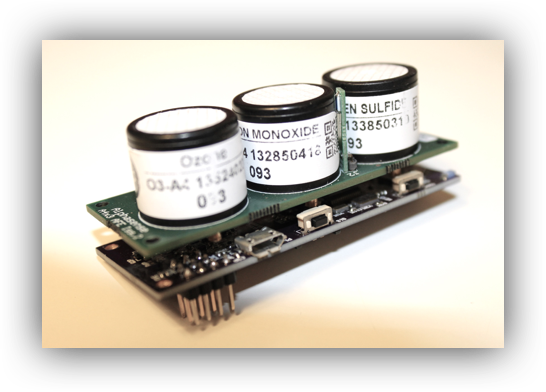
\includegraphics[width=\textwidth]{visuals/learnairV2}               
 	 \caption{Second revision, Atmel based learnAir main board mated with the AlphaSense sensor frontend}
  	\label{fig:learnairV2}
\end{marginfigure}

Two daughter boards were designed to connect with the main board learnAir board.  This modular design gives more flexibility for housing the device, simple upgradability, and separates concerns when testing/verifying the circuitry.  

The first of these daughter boards includes all sensors that need to be mounted on against the edge of the device, either in contact with the air or with direct access to sunlight.  This small board includes a ROHM \textbf{BH1730FVC} I2C light sensor, a Vishay \textbf{VEML6070} I2C UV sensor, and a Sensirion \textbf{SHT25} temperature and humidity sensor.  The SHT25 is similar to the SHT21 used in learnAir V1, but with slightly tighter tolerances. 

The second daughter board is designed to hold three Omron \textbf{D6F-PH} differential pressure sensors, for 3-axis wind sensing.  This is the same pressure sensor as was tested in the learnAir V1 device.  Since the D6F-PH does not come with selectable I2C addresses, this daughter board also has an NXP PCA9545	 I2C-bus switch to selective open the I2C bus between one of the three pressure sensors and the main learnAir board.  This I2C bus switch is itself addressable and controllable over I2C, so no extra pins are required to connect it.  Schematics for both daughter boards can be found in Appendix B.

Besides the connections to the three AlphaSense gas sensors controlled by the AlphaSense Analog Front End board, the main board is also equipped to connect to either a Sharp GP2Y1010AU0F (as tested in the learnAir V1 device) or the much more accurate \$500 AlphaSense \textbf{OPC-N2}.  The OPC-N2 takes advantage of Mie scattering algorithms and uses higher quality optics, but it is insensitive to particles under a few hundred nm and has a limited feature-set around flow filtering and control.  Independent validation of the OPC-N2 has been mixed, and the device includes a built in fan (demanding a lot of power for a portable device), but it offers an enticing combination of cost and size given its sophistication.

A final physical design of the learnAir V2 device was modeled in SolidWorks, and fits in the palm of a user's hand (Figure \ref{fig:learnairbox}).  The final cost of the OPC-N2 version is around \$1k, while the Sharp version is closer to \$600.  

\begin{figure}[htb]
 	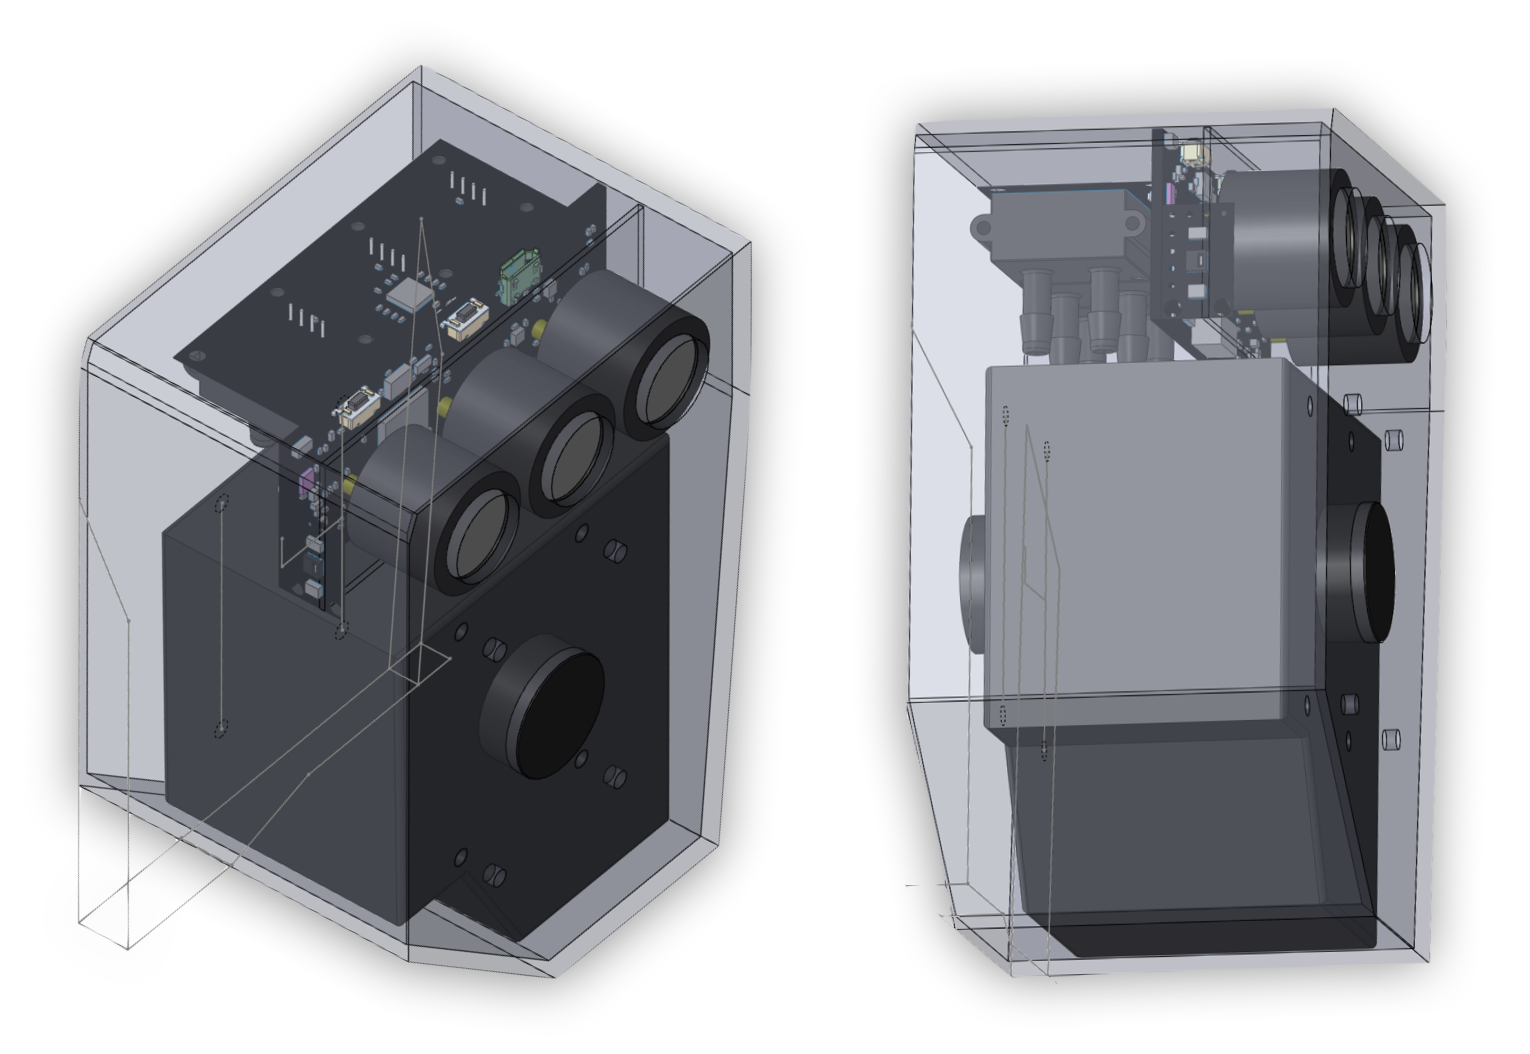
\includegraphics[width=\textwidth]{visuals/learnairV2box}               
 	 \caption{Final design of the portable system}
  	\label{fig:learnairbox}
\end{figure}

Once the hardware was actually designed and built, firmware to control the device needed to be created.  The Arduino environment and libraries were used to write code for learnAir V2.  Since this is a demanding application, the standard pinouts used by typical Arduino boards needed to be redefined.  LearnAir clocking and custom pin mapping definition files were added to the Arduino environment-- now, similar to `Leonardo' and `Due' and other boards, the `learnAir' board can be chosen and programmed as an option from the Arduino environment dropdown menu.  Firmware and board definition code is available in Appendix B.  The completed code and hardware was tested with a learnAir smartphone application and shown to work reliably.

\FloatBarrier

\begin{figure}[htb]
 	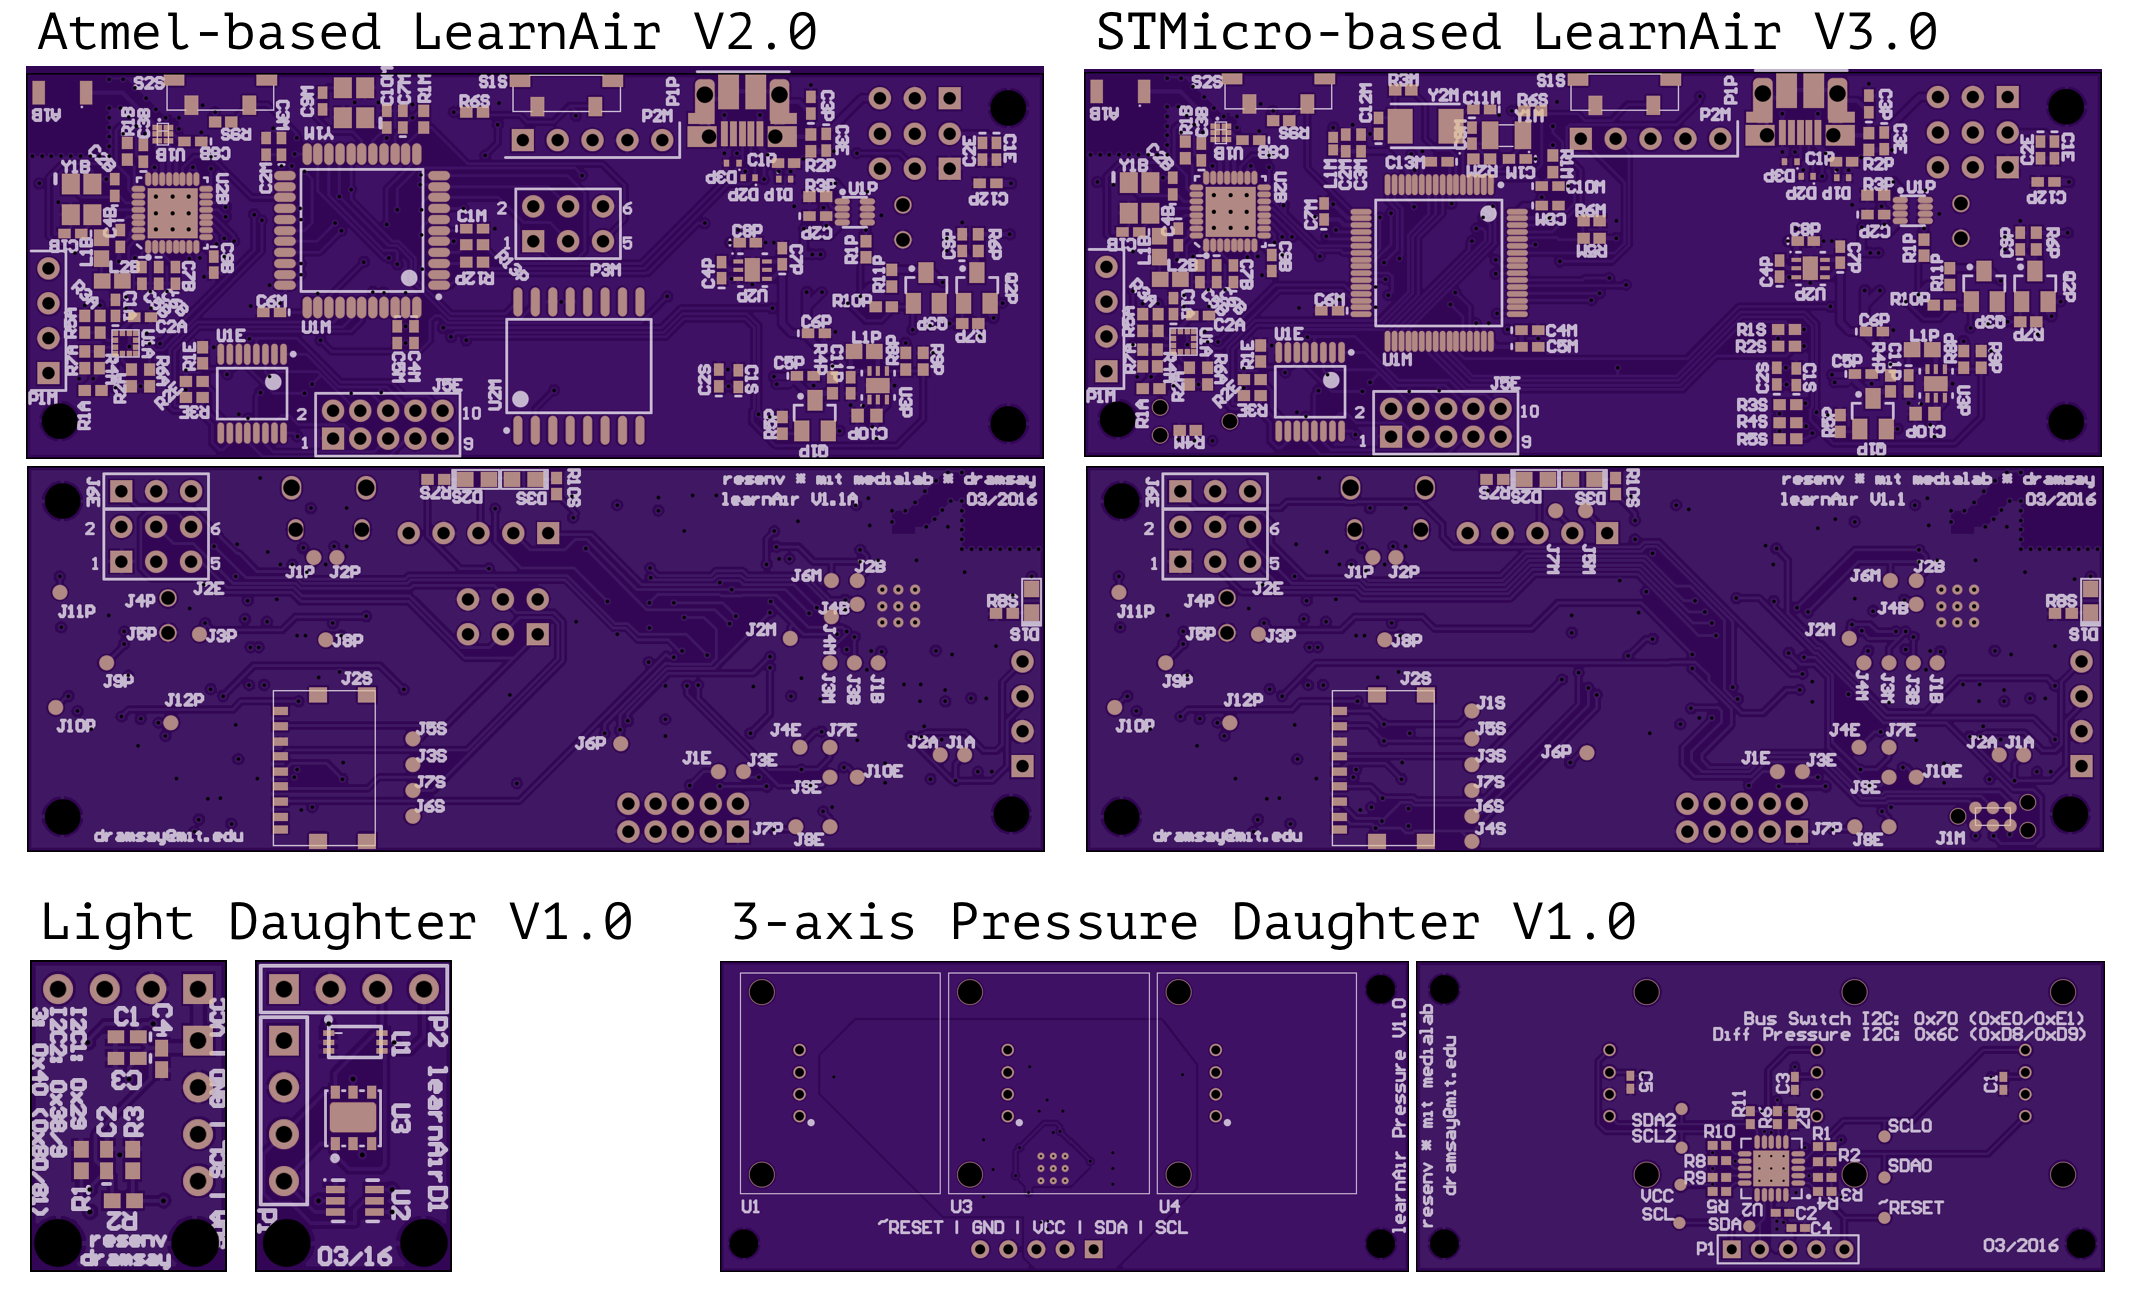
\includegraphics[width=\textwidth]{visuals/layouts}               
 	 \caption{Layouts for revisions 2.0 and 3.0 of the learnAir board}
  	\label{fig:layouts}
\end{figure}


\FloatBarrier
\section{LearnAir Version 3}
\FloatBarrier

The third version of learnAir hardware is very similar to the second in most ways.  It supports the same daughter boards, peripherals, power circuitry, USB charging/communication, accelerometer, and bluetooth communication.  The main difference is the choice of microprocessor-- this time, the ST Micro STM32L152 was used.  This processor is much more advanced than the Atmel chip built into version 2-- it offers more a elegant programming interface, it has higher resolution ADCs (12-bit instead of 10-bit), it runs at much lower power and with many advanced power-handling features, it includes advanced features like an on-board RTC and a fully parallel SDIO interface, it has extensible and powerful code support, and it brings the entire board down in price.  

While it is able to connect to the existing wind daughter board, this hardware includes an experimental differential pressure sensor (for wind measurement) on the main learnAir board itself.  This is a cutting edge MEMS differential pressure sensor-- the Sensirion \textbf{SDP31}-- which is not yet publicly available.  While it performs similarly the Omron D6F-PH, it is dramatically smaller-- 8.5 x 5.5 x 4.4mm (600 mm$^3$) vs. the Omron's 26 x 18 x 22mm (31,000 mm$^3$).  This is a huge reduction in size for the learnAir system.

The STM32L152's onboard RTC also saves in cost and layout space compared with version 2.  The fully parallel SDIO interface is helpful for power savings-- SD Card data can be written over SPI (with two data lines) or over this 4-pin parallel bus.  SD Card writes are power hungry, so it is useful for low-power operation to be able to minimize write time by maximizing the parallelization of data transfer.  BLE transfer also requires bursts of power-- it is valuable to be able to store data on-board and batch-send it to the phone or over USB, especially if the device's battery is low.  Additionally, the extra SPI and I2C buses allow parallelization, which means we can cut our duty cycle down.  This type of advanced power optimization is a goal of learnAir V3.

Power consumption for both boards is dominated by SD card writes, BLE, and high power peripherals.  Rough power estimates of each system show the LearnAir V2 system requiring around 5 mW of power (attached to the Sharp sensor with a 30 second duty cycle), and the V3 system requiring around 3.5 mW.  Since the OPC-N2 is a relatively high power device, and must be left on for at least one second to acquire a reading (unlike every other sensor in the system), if it is connected it completely dominates our power estimates.  Both systems require an order of magnitude more power with the OPC-N2 included (35-40 mW).  These are very rough estimates and a measured power characterization is required for meaningful claims-- it is safe to say, however, that with a several hundred mAh LiPo battery we can expect a battery life of several days to several weeks, depending on the attached peripherals and duty cycling of the device.      

\enlargethispage{10\baselineskip}

The V3 version-- while built and tested-- still requires a few extra support libraries to be ported over before it is smart-phone ready.  Firmware for the ST Family is much more complicated, and requires much more thorough understanding of documentation and setup to optimize it for truly low-power operation.  The build process and configuration of the board, its programming, and basic measurement and output controls have all been successfully tested with this design.  It represents a major step toward true production-quality.  Schematics and code samples can be found in Appendix B.

\begin{figure}
 	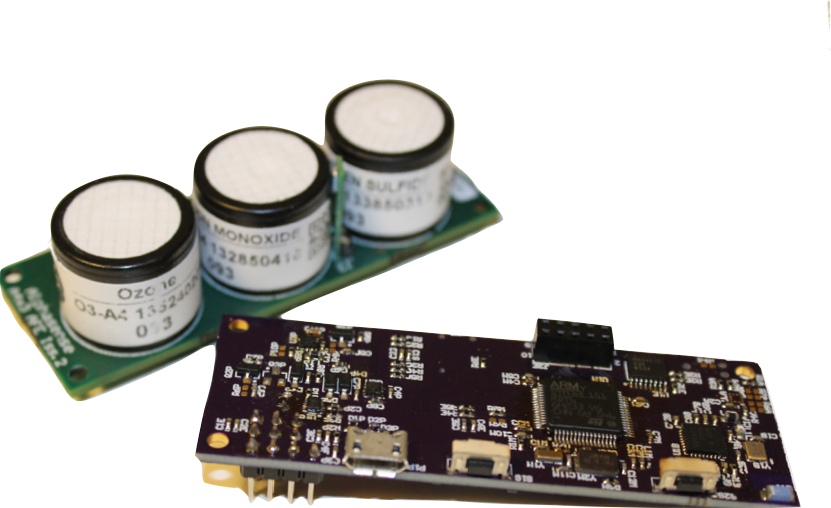
\includegraphics[width=\textwidth]{visuals/learnairV3} \centering              
 	 \caption{Third revision, STM32L152-based learnAir main board next to the AlphaSense sensors}
  	\label{fig:learnairV3}
\end{figure}

\clearpage

\FloatBarrier
\section{Hardware Comparison and Analysis}
\FloatBarrier

MassDEP hardware uses robust, FEM certified techniques-- thus it can be taken as a grounded reference over the time-scales it measures.  The corresponding air quality sensors in the learnAir system are variable in quality, and their analysis is discussed in Chapter 7.    Most of the remaining sensors included in the learnAir system are robust and well-characterized for their purpose.

To validate proper function, in this section we compare temperature and humidity readings from the learnAir device against corresponding weather API data retrieved from ForecastIO for the latitude and longitude of the device.  We also analyze and compare our experimental differential pressure wind sensing design against the ground-truth MassDEP wind speed and wind direction.

ForecastIO data is hourly, and a 60 minute rolling average is used to interpolate the values to the minute timescale.  LearnAir data is collected every minute.

\subsection{Temperature and Humidity}
\FloatBarrier

\begin{marginfigure}[5cm]
 	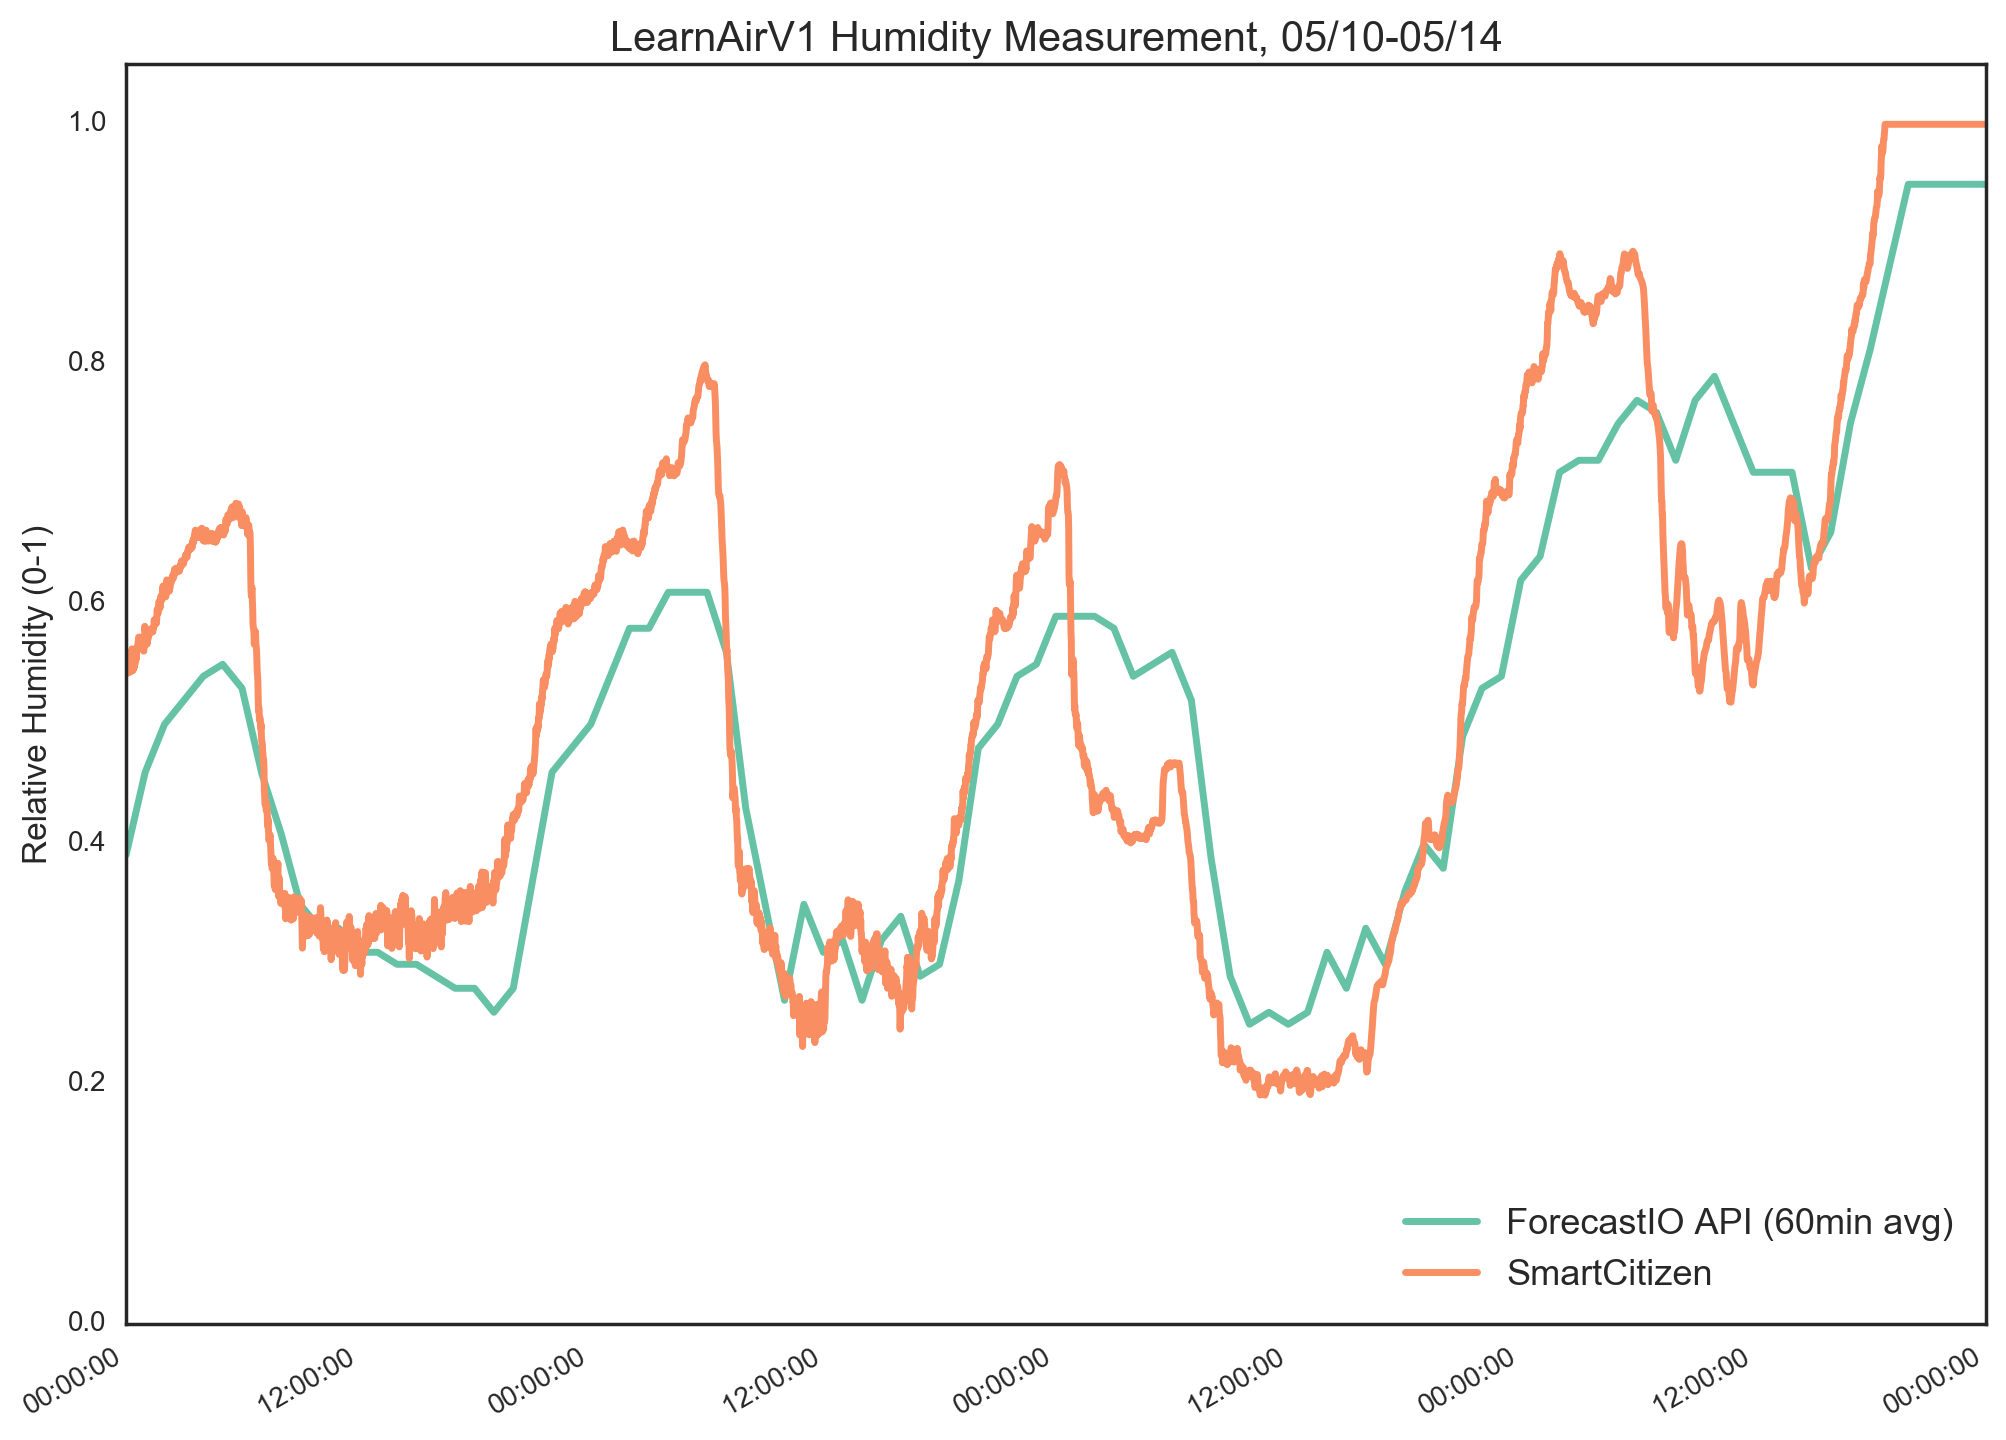
\includegraphics[width=\textwidth]{figs/humidity_zoomed}               
 	 \caption{Humidity Comparison of SmartCitizen (orange) and ForecastIO (green) over 4 days}
  	\label{fig:humidity_zoomed}
\end{marginfigure}

Humidity was recorded in the box by the SmartCitizen Kit and compared against the ForecastIO reading.  Figure \ref{fig:humidity_sck_v_forecastio} shows a comparison of each SmartCitizen reading with each ForecastIO value-- ideally they would track closely, falling on the 1:1 line when plotted against each other.  Instead we see a slight skew towards higher humidity in the box.  It is reasonable to assume this is a real phenomena-- temperature differential in the box may cause condensation and elevated humidity.  In either case, the consistency between the measurements is quite good, and suggests trustworthiness. 

\begin{figure}[htb]
 	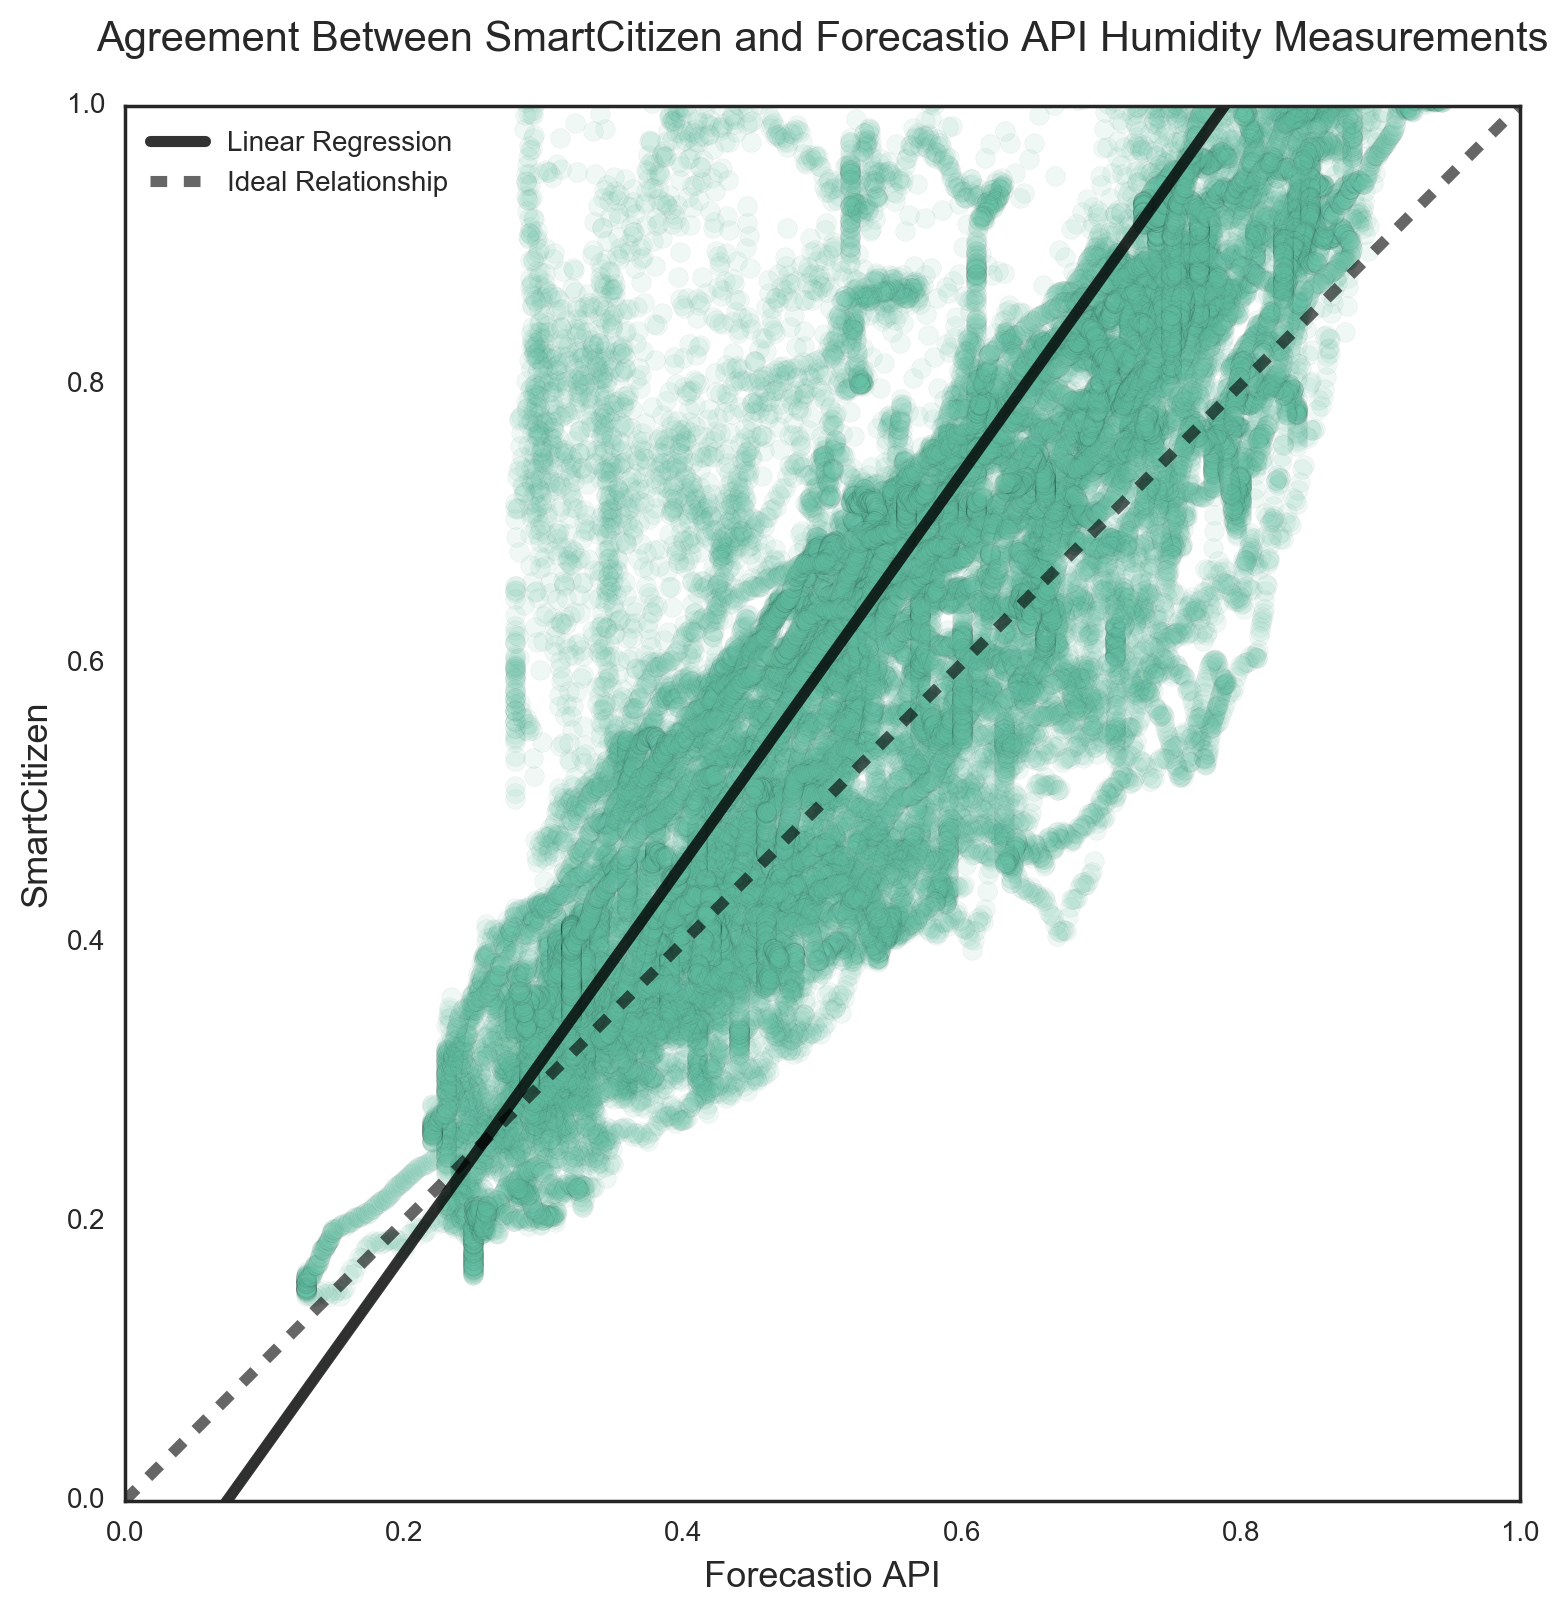
\includegraphics[width=\textwidth]{figs/humidity_sck_v_forecastio}               
 	 \caption{Humidity Comparison, SmartCitizen and ForecastIO}
  	\label{fig:humidity_sck_v_forecastio}
\end{figure}

\begin{marginfigure}[3.5cm]
 	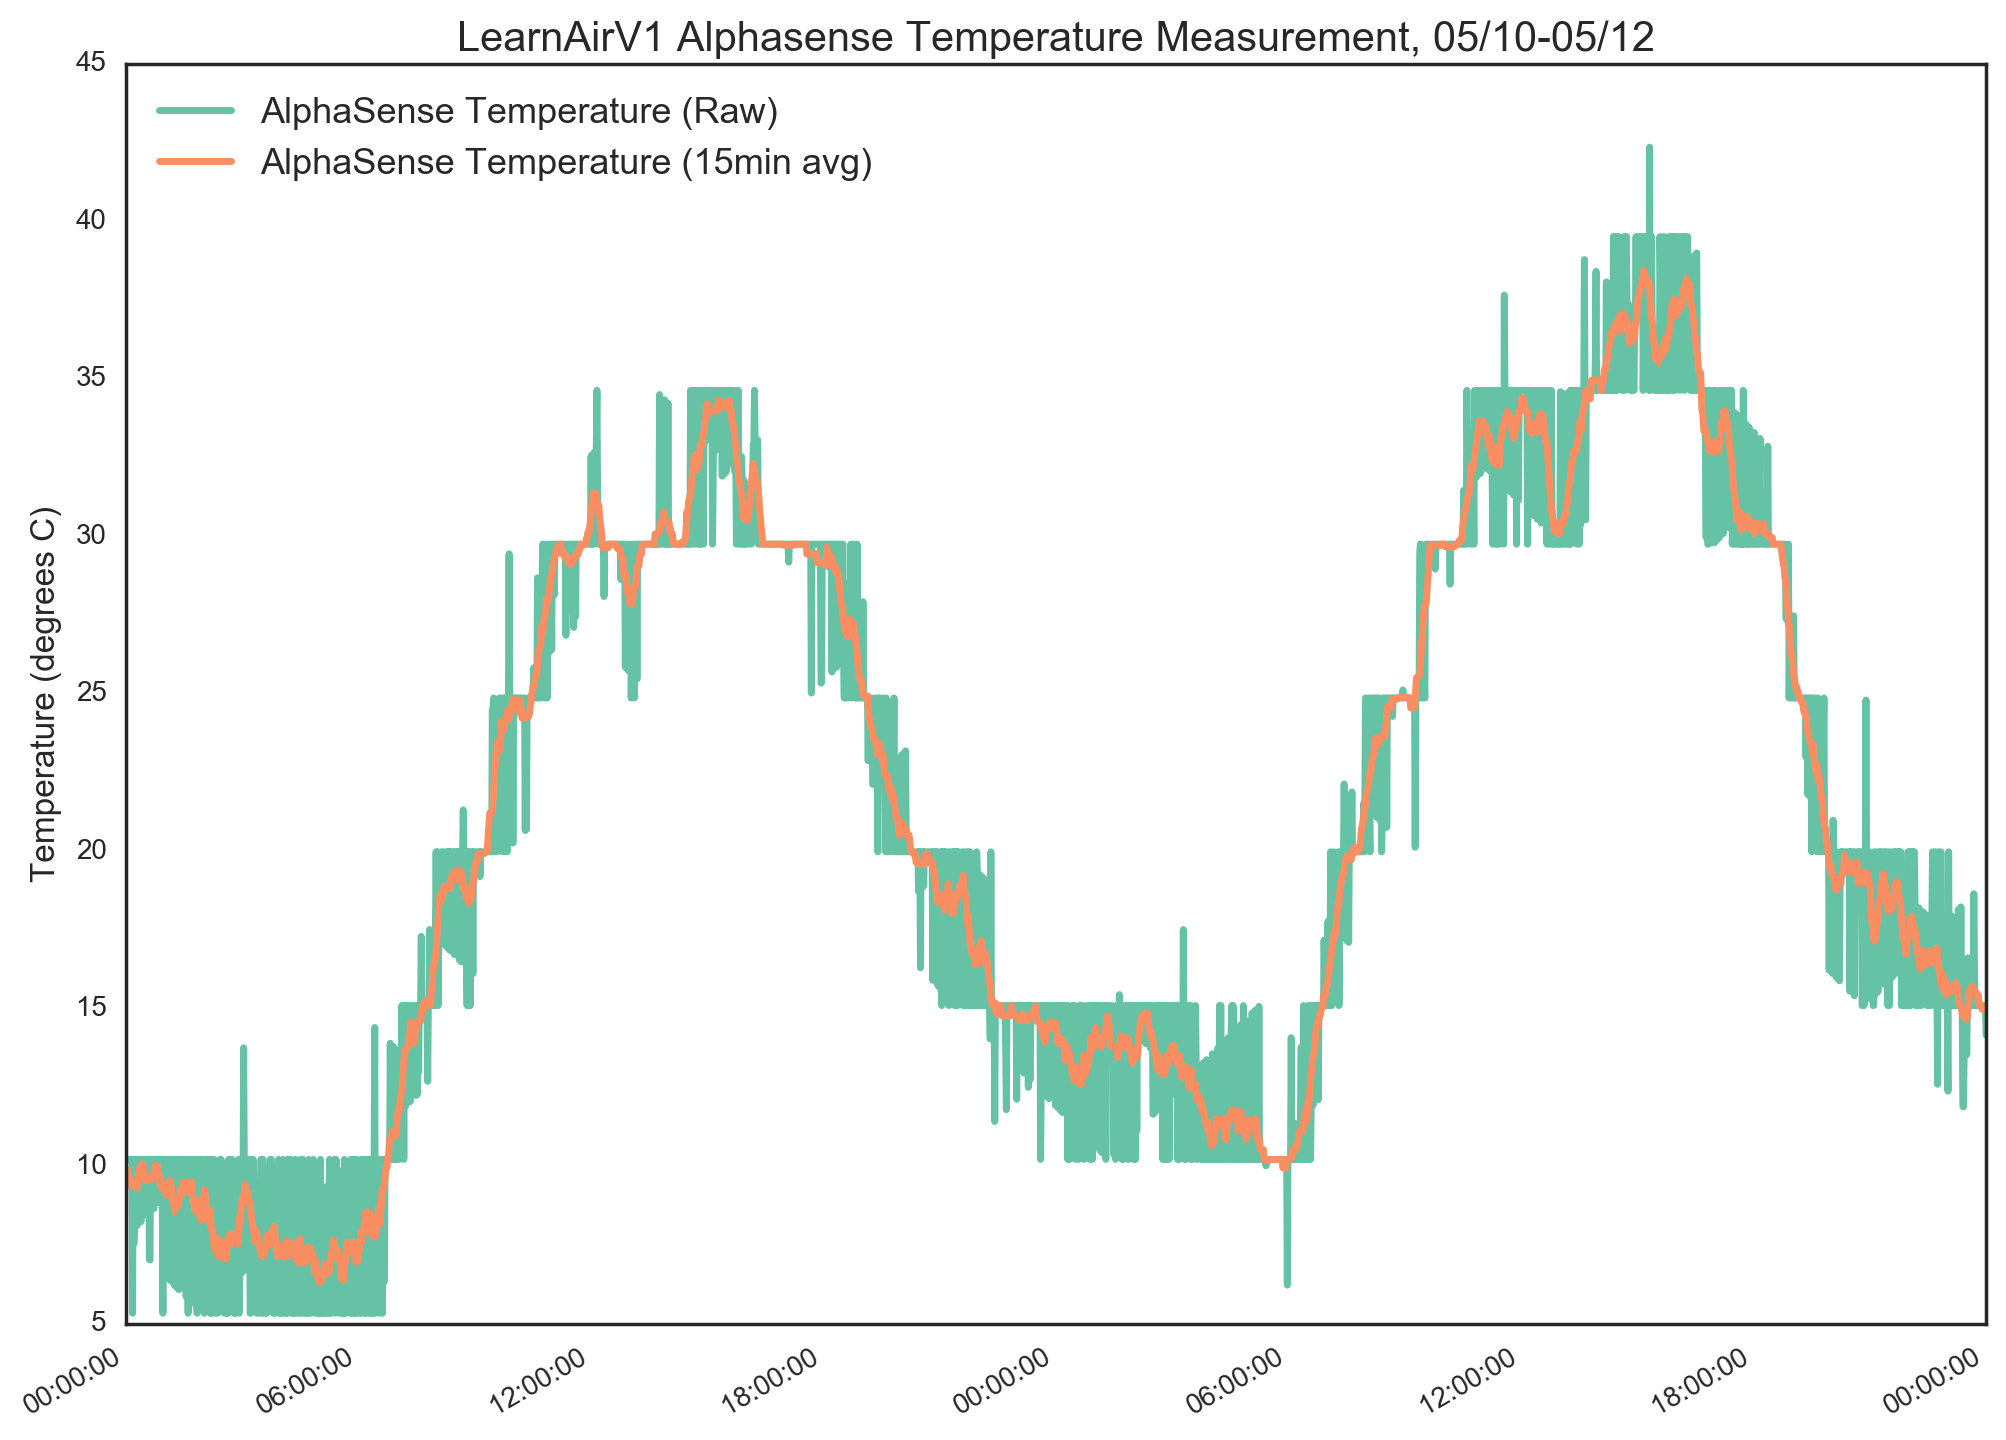
\includegraphics[width=\textwidth]{figs/temp_alphasense}               
 	 \caption{Alphasense Raw Temperature Data (green) with 15-minute averaging (orange)}
  	\label{fig:temp_alphasense}
\end{marginfigure}


Temperature was recorded inside the box by both the AlphaSense temperature sensor and the SmartCitizen Kit.  Figure \ref{fig:temp_alphasense} shows quantization error on the raw AlphaSense reading (teal)-- this is mitigated by taking a 15-minute rolling average (orange).  In Figure \ref{fig:temp_zoomed} we see a four day comparison of ForecastIO data with data taken in the box from the AlphaSense and SmartCitizen sensors.    We see good agreement between in-the-box data, with some slight variation as temperatures exceed 25 degrees Celcius.  There is also good agreement between the ForecastIO data and the in-the-box data when the sun is down.  This is a real effect-- the learnAir box was exposed to direct sunlight, and thus shows significant rises in temperature during the day compared with ambient conditions.  Both temperatures (and their differential) are used to as features for our machine learning algorithm, with in-the-box temperatures informing our calibration process (which is appropriate as the air quality sensors are likewise in the box).   

\begin{figure}[htb]
 	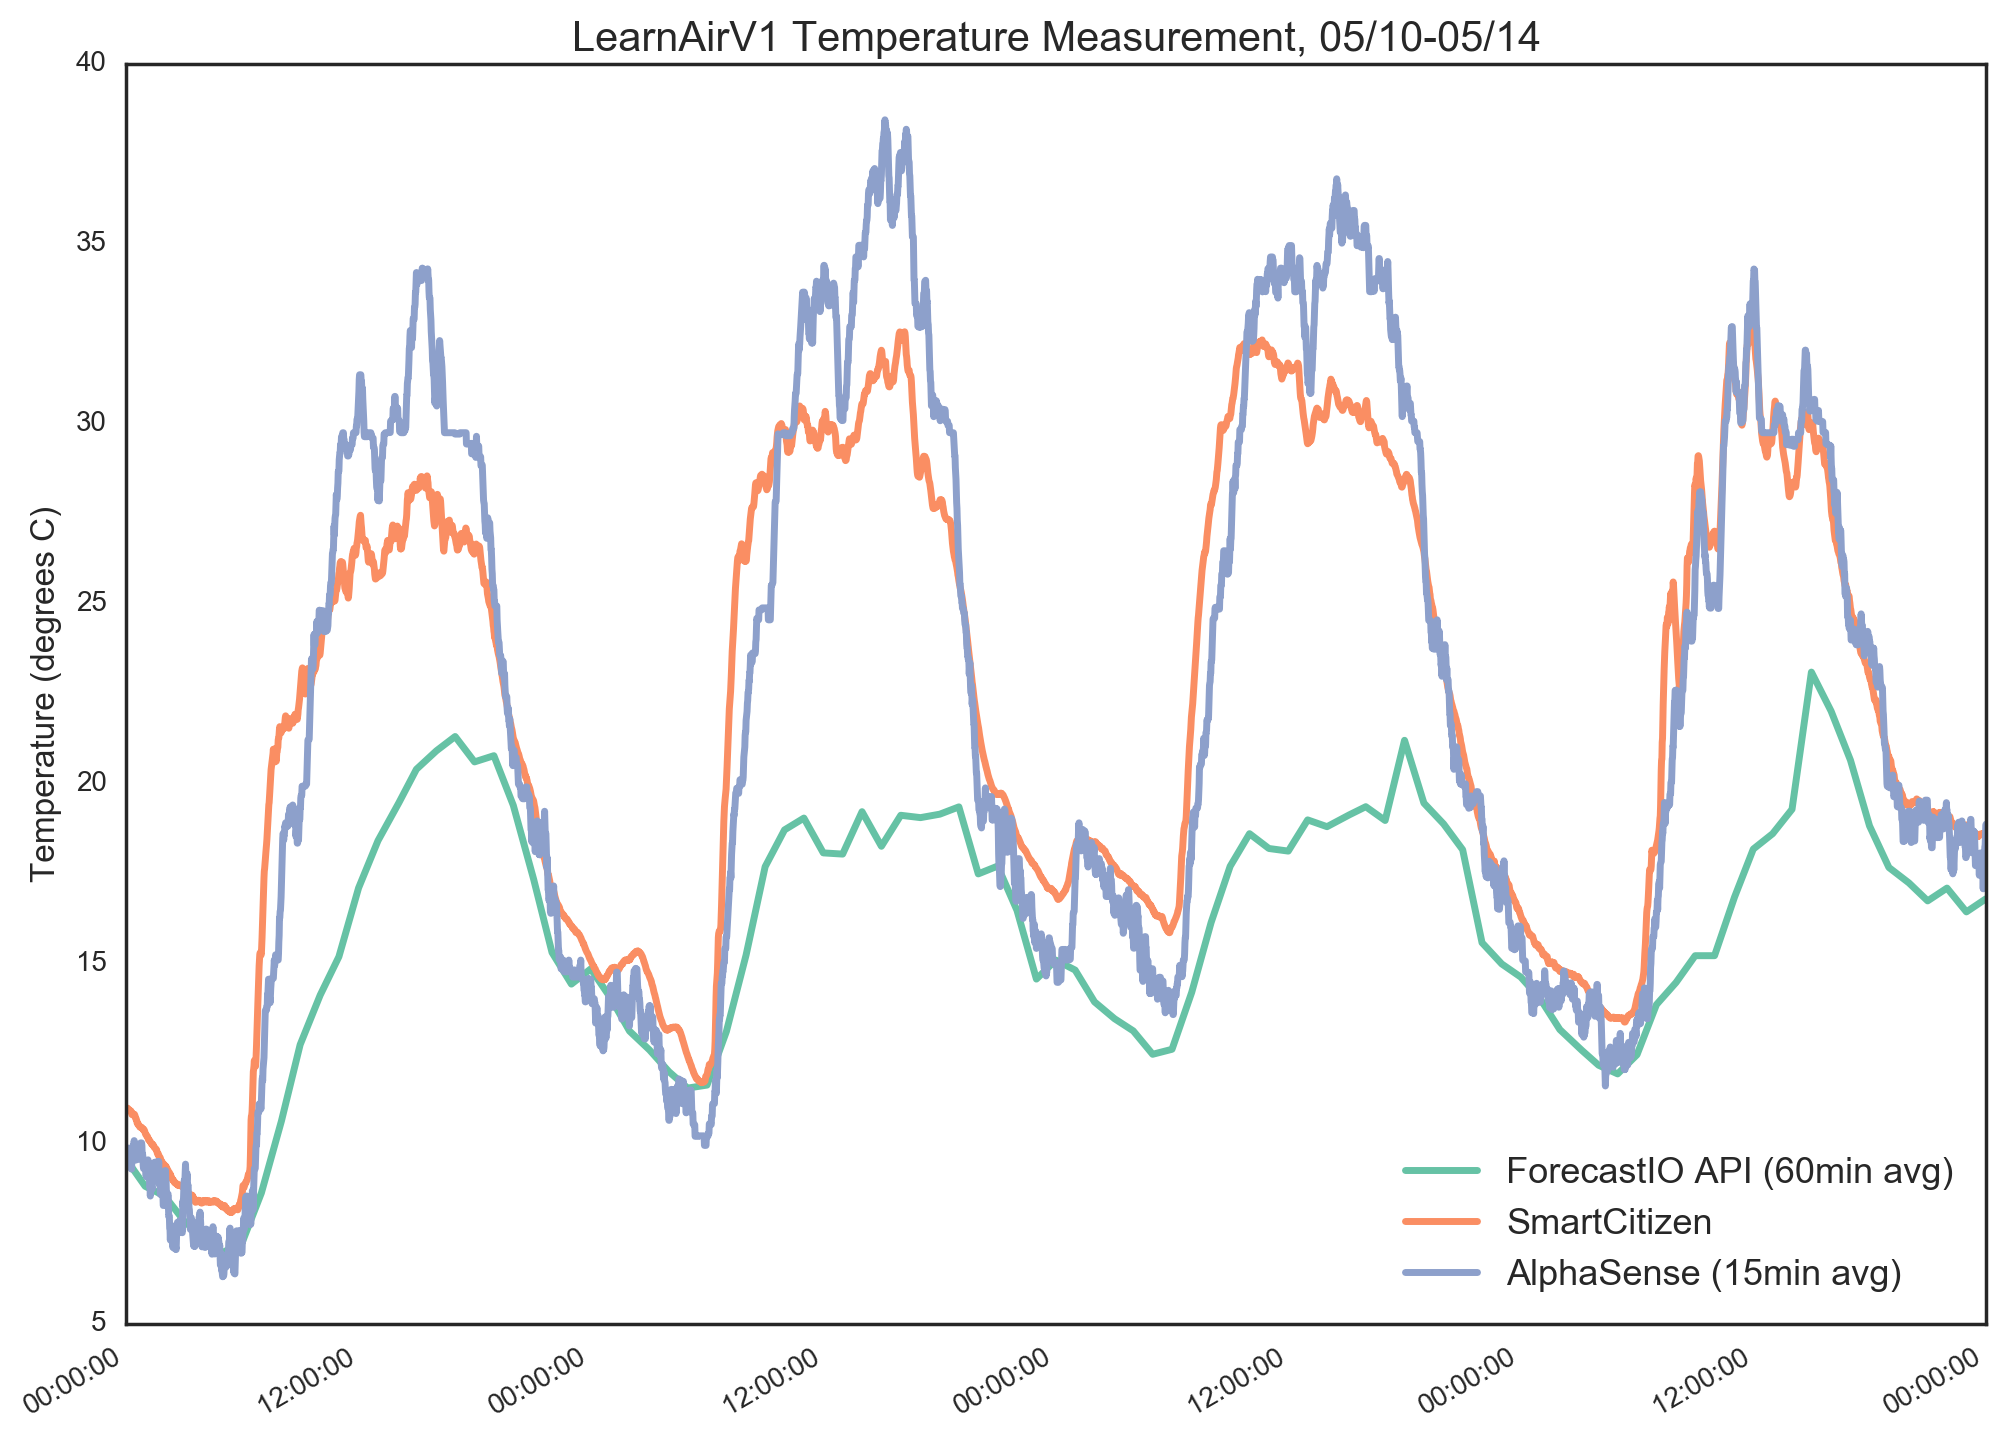
\includegraphics[width=\textwidth]{figs/temp_zoomed}               
 	 \caption{Temperature close-up}
  	\label{fig:temp_zoomed}
\end{figure}

\begin{marginfigure}[3.5cm]
 	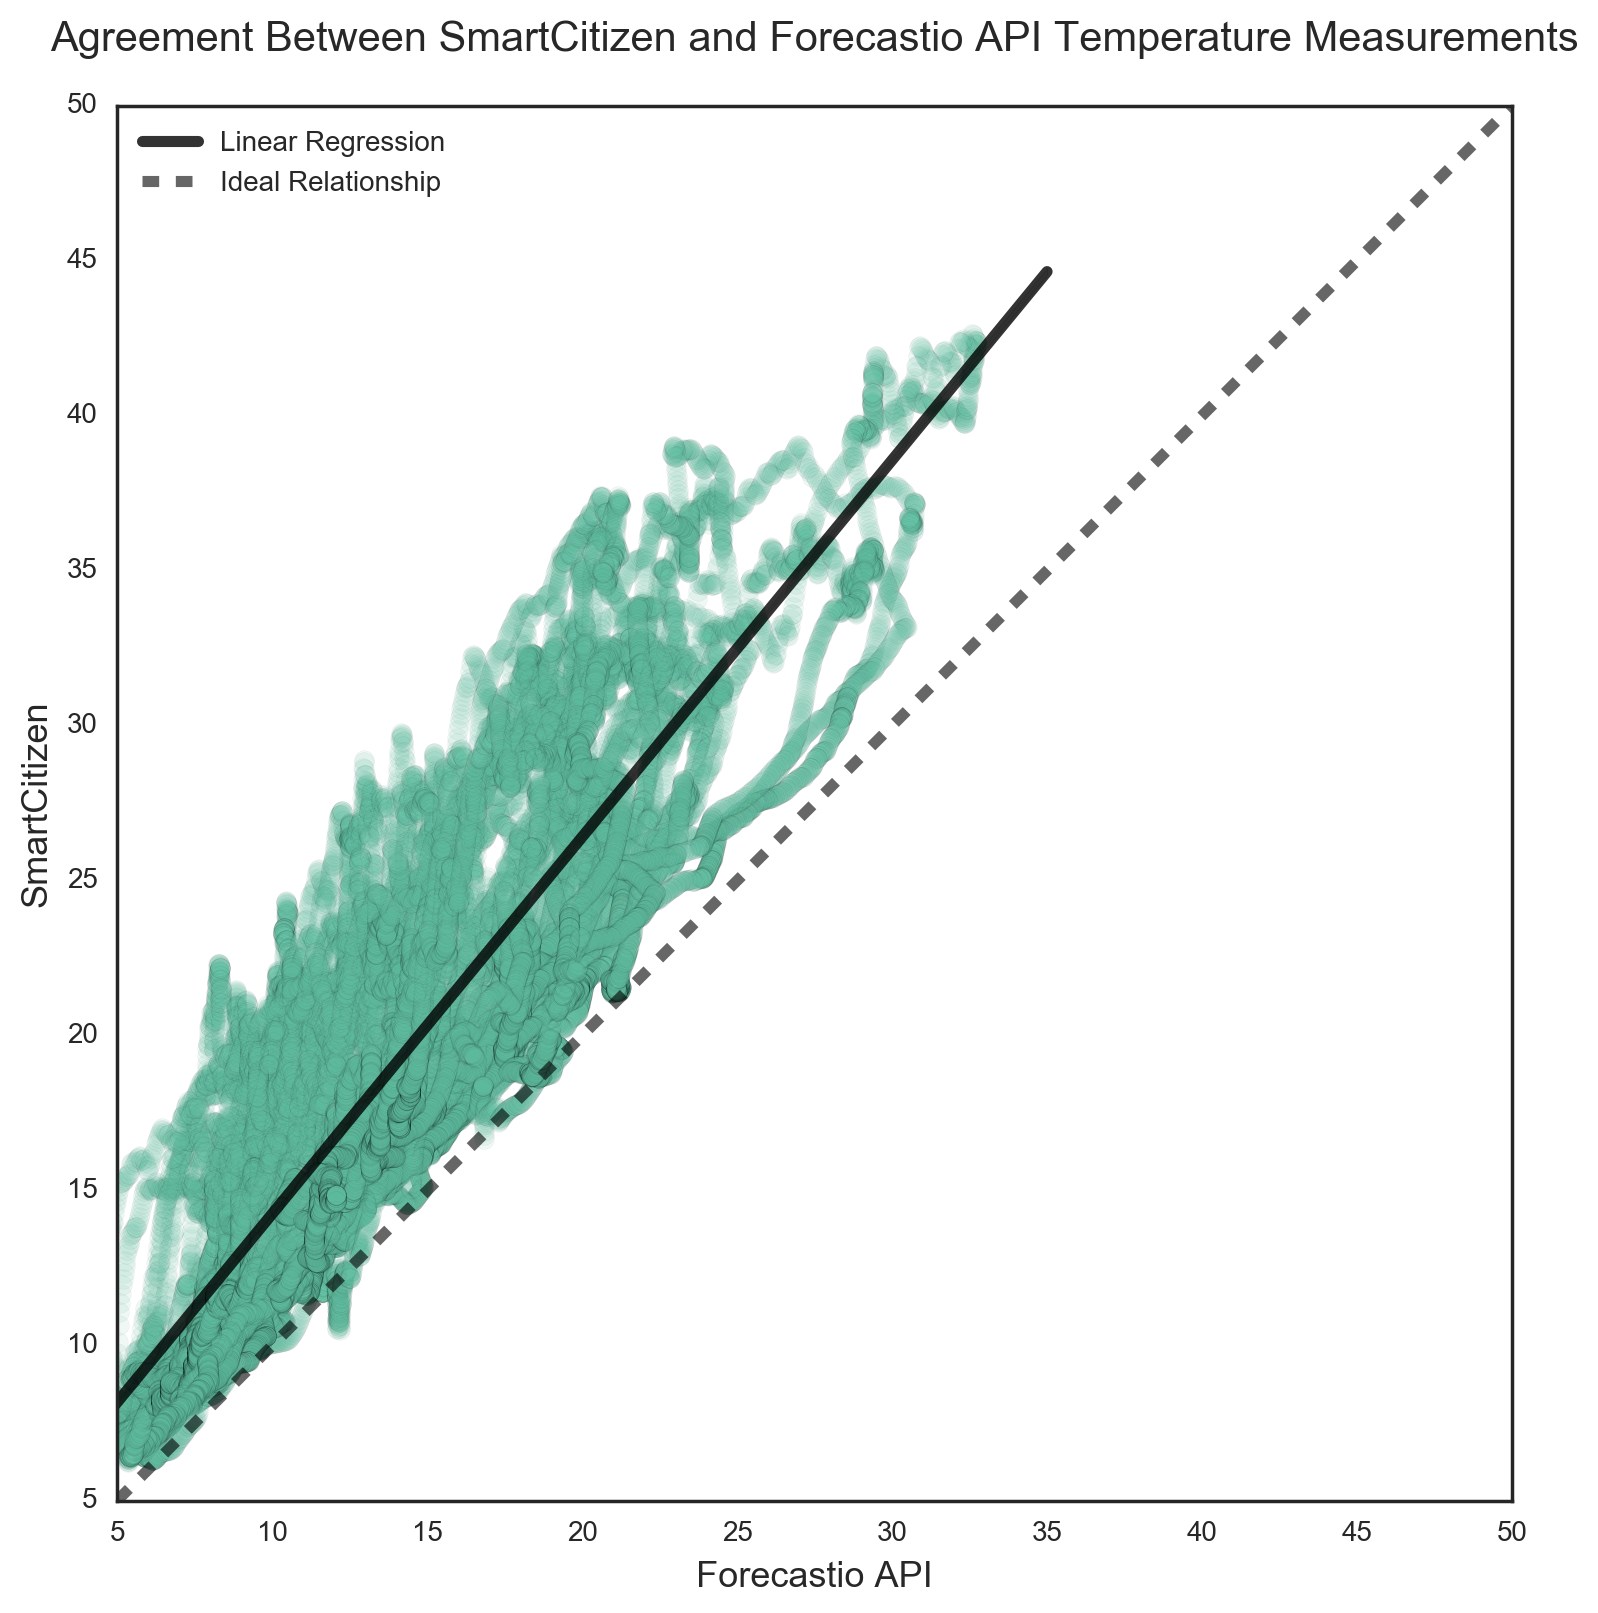
\includegraphics[width=\textwidth]{figs/temp_forecastio_v_sck}               
 	 \caption{Temperature Comparison, SmartCitizen and ForecastIO}
  	\label{fig:temp_forecastio_v_sck}
\end{marginfigure}

\subsection{Wind}
\FloatBarrier

Using differences in pressure to sense wind direction is not a new concept-- pitot tubes (frequently found on airplanes) are one such example.  Recent work to create MEMs wind sensors using this modality has also started to appear. \cite{wind}  It is not typical to find differential pressure sensing used in this way, however; particularly at this scale, and taking into account (or potentially leveraging) the geometry of a larger box.

Thus, the included differential pressure sensor was a small, cheap, and experimental way to measure airflow and wind through the device.  One of its two ports is connected to the side of the box with a tube, while the other is vented into the box-- since the box has holes and is pressure equalized, any differences we measure can be attributed to wind on the outside box face.  While the learnAir V1 sensor only had one differential pressure sensor in it (mounted on the same face as the other sensor inlets), the boards were designed to support three axis sensing, in order to get a truly 3-D understanding of wind speed and directivity and how that may affect air quality measurement.  Doing so accurately requires polar pattern analysis, orthogonality in wind response vs. direction, and some interesting device geometry and signal processing.  This is an open research question in and of itself.  In this first instance, only one axis (measuring speed and not direction) was captured on the primary face of the device.

As a first step to explore the feasibility of such a wind sensing system, the learnAir system was (1) characterized using a home-made laminar flow setup, and then (2) compared against trustworthy external wind speed and direction data from MassDEP.  

The goal of the first test was to get a sense for learnAir's wind direction selectivity.  Since the design is rectangular and the wind sensor is protected by a slotted design, we would expect air flow parallel with the slots to penetrate less than perpendicular flow.  We'd also expect air coming directly at the sensing face of the device to penetrate much more than air flow coming at the back.

\begin{marginfigure}
 	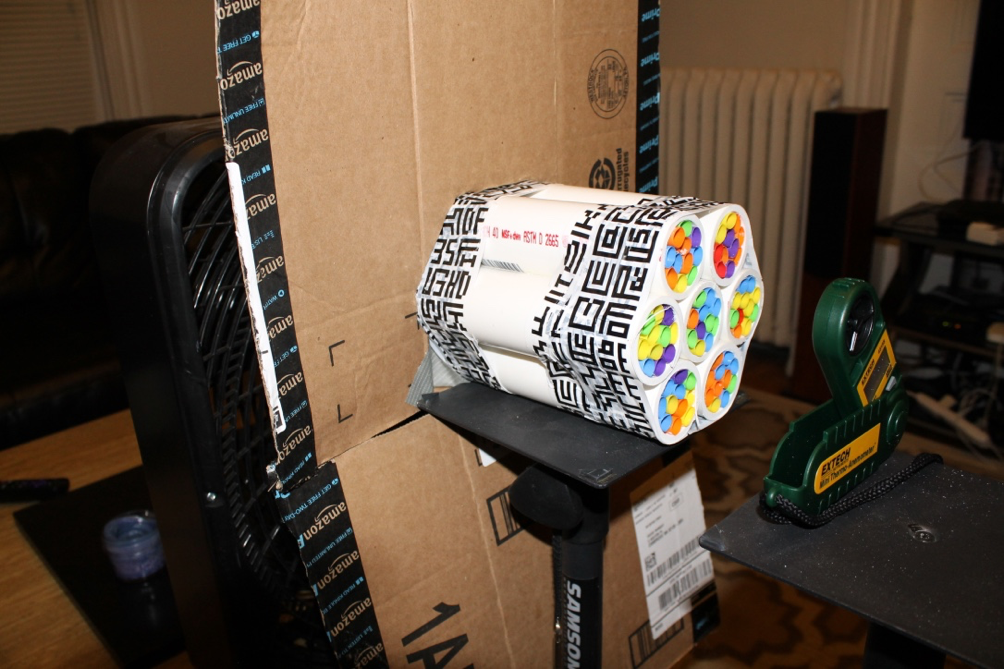
\includegraphics[width=\textwidth]{visuals/windtest}               
 	 \caption{A picture of a simple laminar flow test setup for rough wind directivity characterization}
  	\label{fig:windtest}
\end{marginfigure}

\enlargethispage{2cm}


To test this, PVC pipes filled with large straws was placed in front of a fan to approximate laminar flow conditions (Figure \ref{fig:windtest}).  Cardboard was placed around the laminar flow section to prevent spurious eddy currents.  A handheld Extech 45158 Anemometer was used to validate a constant airflow of 2 m/s (a light breeze).  The learnAir V1 device was then placed in the flow, and rotated at 30 degree intervals, with 10 wind measurements at each interval.  The top half of figure \ref{fig:wind_polar} shows a normalized polar response with air flowing directly towards the slotted wind sensor device face at 0 degrees (and directly at the rear face of the device at 180).  The bottom half shows the response of the device with wind flowing over top of the face at various angles-- 0 degrees represents airflow parallel with the short dimension of the learnAir box, and 90 degrees is parallel with the long dimension.

\begin{figure}[htb]
 	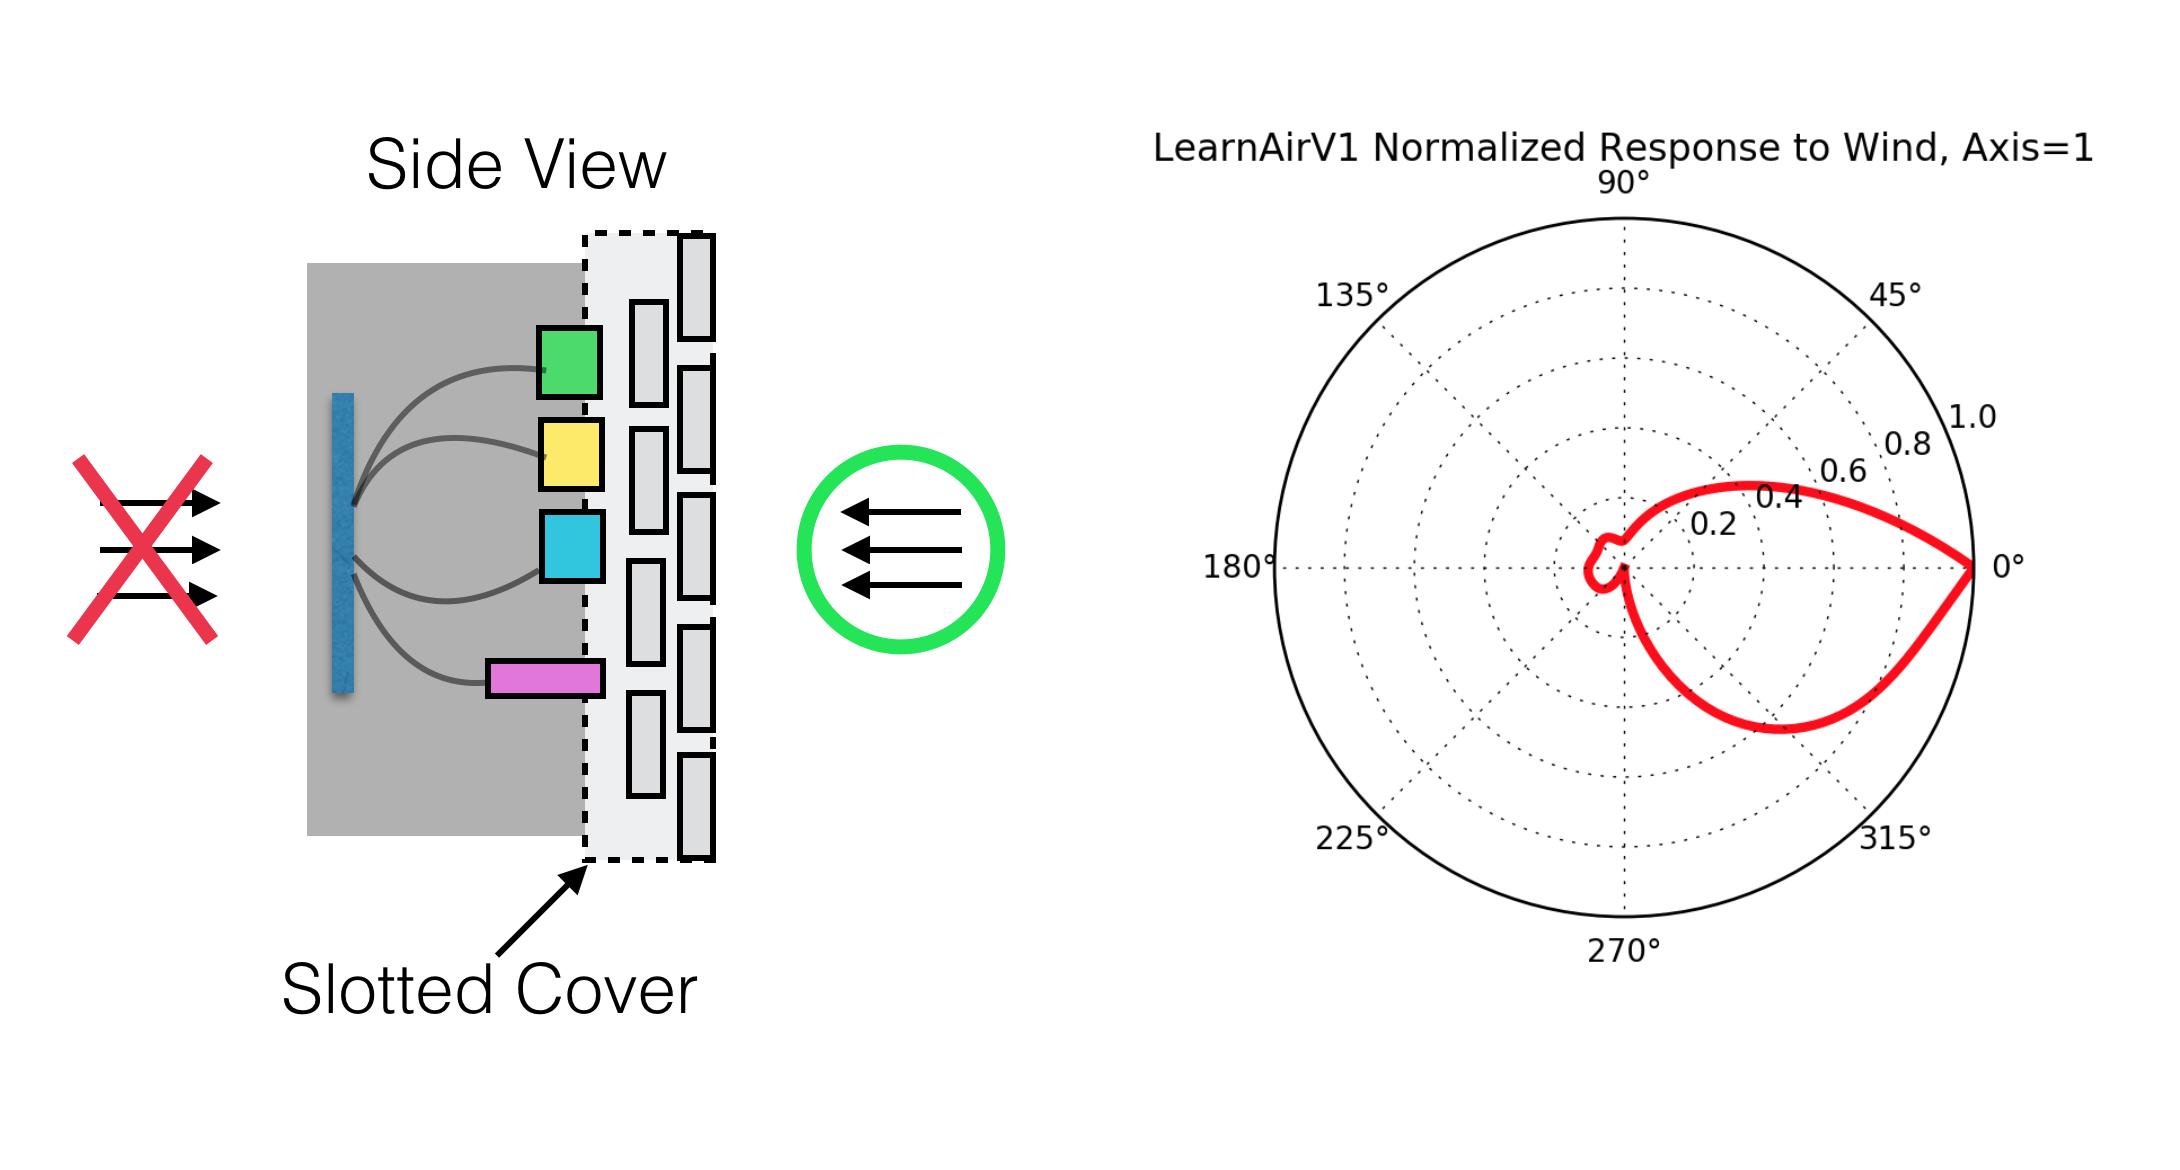
\includegraphics[width=\textwidth]{figs/wind_polar_1}               
 	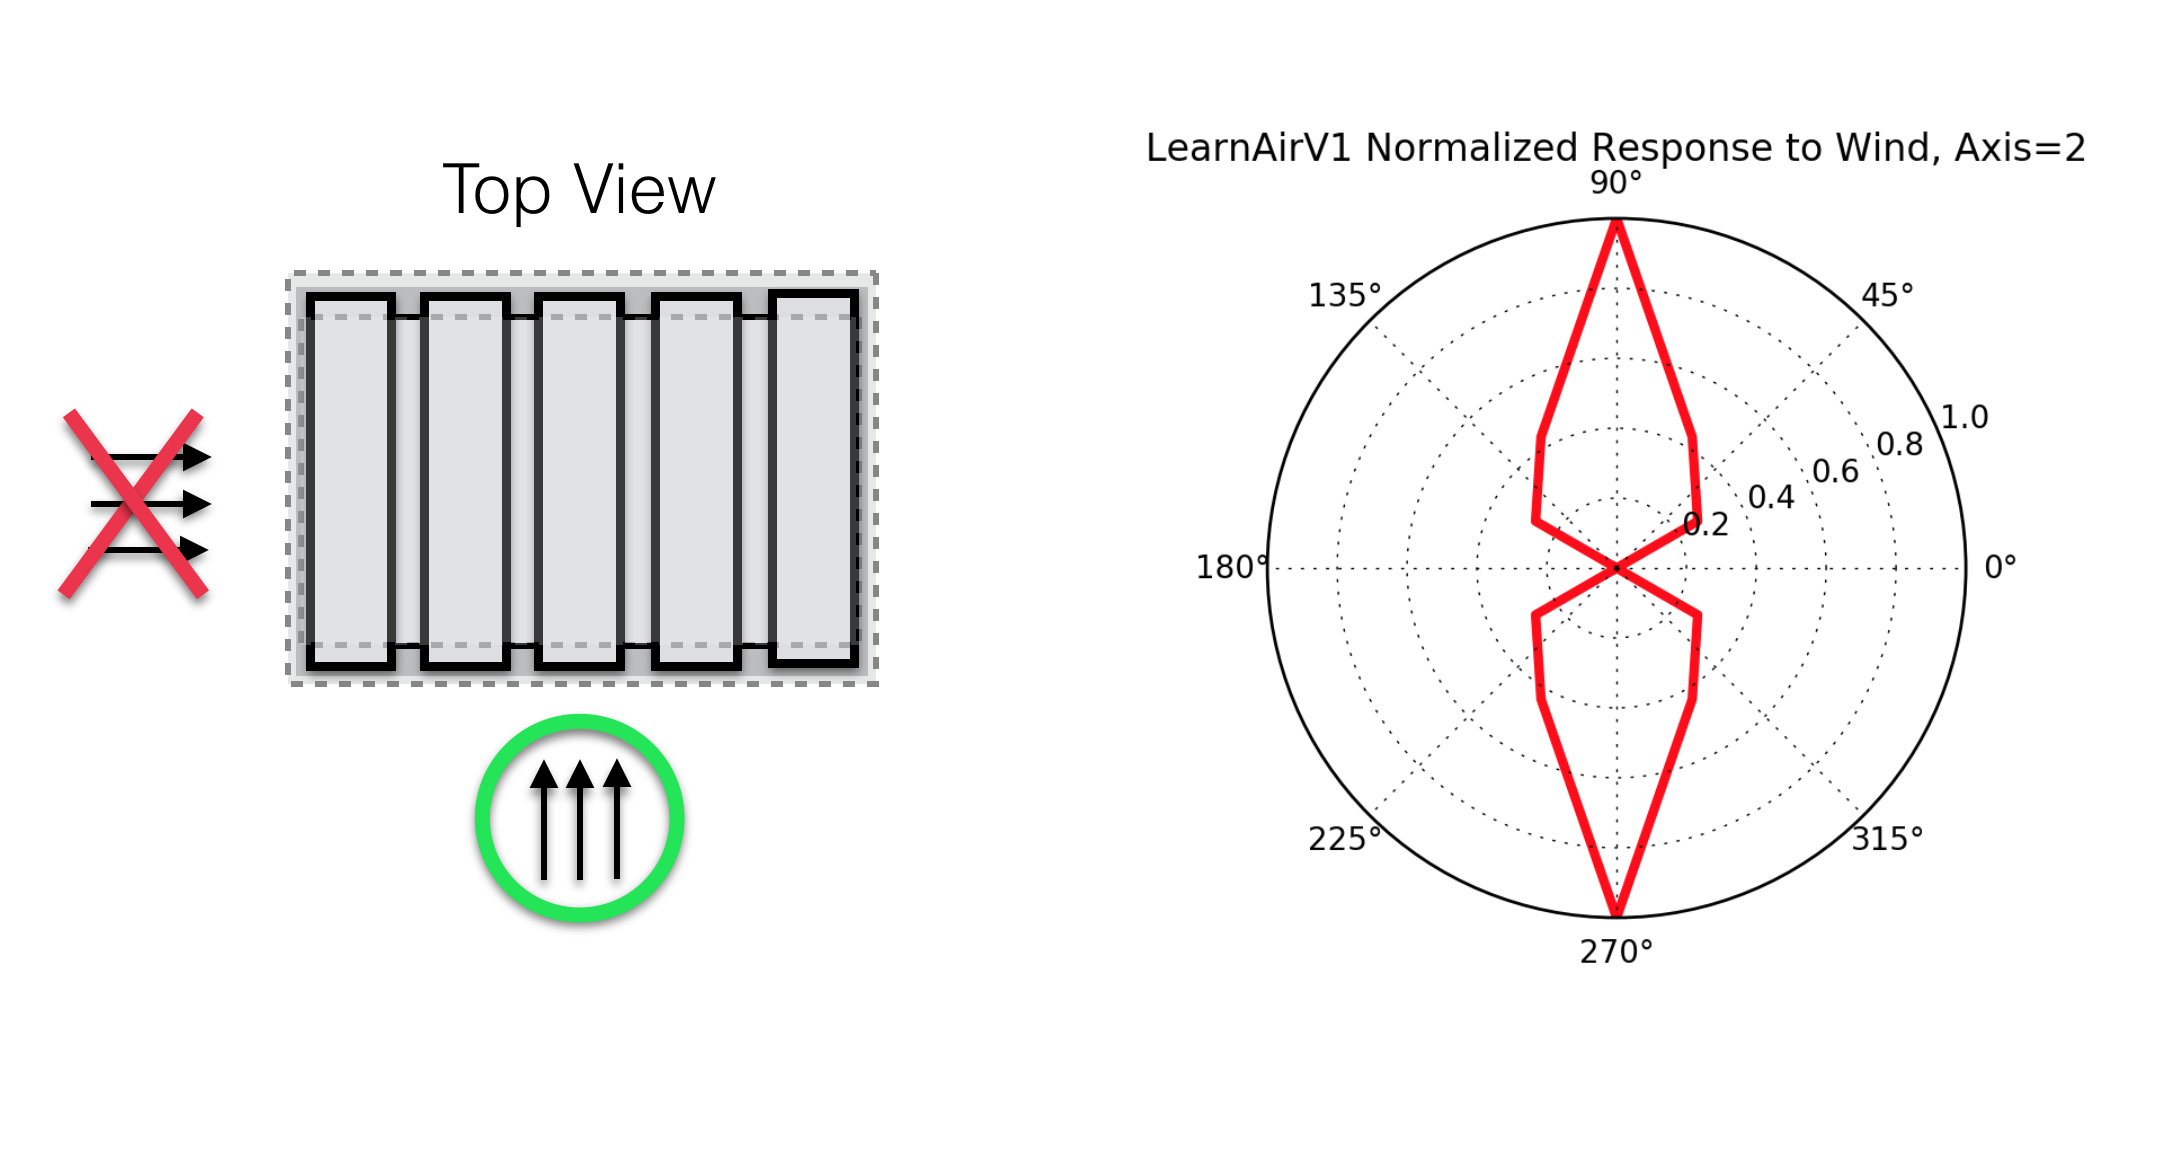
\includegraphics[width=\textwidth]{figs/wind_polar_2}               
 	 \caption{Wind Directivity Polar Patterns}
  	\label{fig:wind_polar}
\end{figure}

As expected, the device responds with an interesting 3 dimensional pattern.  It is very responsive to airflow coming at the face, and very insensitive to air flow coming from behind.  It is very sensitive to airflow perpendicular to its slots, and completely insensitive to airflow that is parallel.  This is a very useful feature to exploit for truly three dimensional wind sensing, and for controlling device airflow.  Designs that include checkerboard slots or slots in both directions may be very impervious to wind.  At the same time, with no active airflow through the device, these results suggest that the air that is being sampled is (1) more likely to be pushed into the cavity from specific directions, which may artificially affect how sensitive to directional sources of pollutions like a nearby road, and (2) we may expect some low-pass filtering effects relative to a sensor design that actively pulls air through the device, especially when the wind is blowing in a direction that has difficulty penetrating the slotted cover. 

\pagebreak

The second test compares windspeed measured by the device with windspeed measured externally by the MassDEP sensor.  We would expect, given our polar plots, that (1) the actual airflow we're sensing is different/shielded from the real wind, so there may be some differences in the measurement, and (2) our device is selective to certain wind directions, so it is important to analyze the relationship of errors in our readings compared with the MassDEP readings as a function of wind direction. 

Figure \ref{fig:ws_with_10_accuracy_zoomed} shows a comparison of measured windspeed data from our pressure sensor against the MassDEP data for one day (after pre-conditioning the signal and LMSE scaling it against the MassDEP reference).  There is a clear correlation in overall trend, suggesting the pressure sensor is capturing meaningful information.  Tight agreement of $\pm$5\% between readings is highlighted in green.   

\begin{figure}[htb]
 	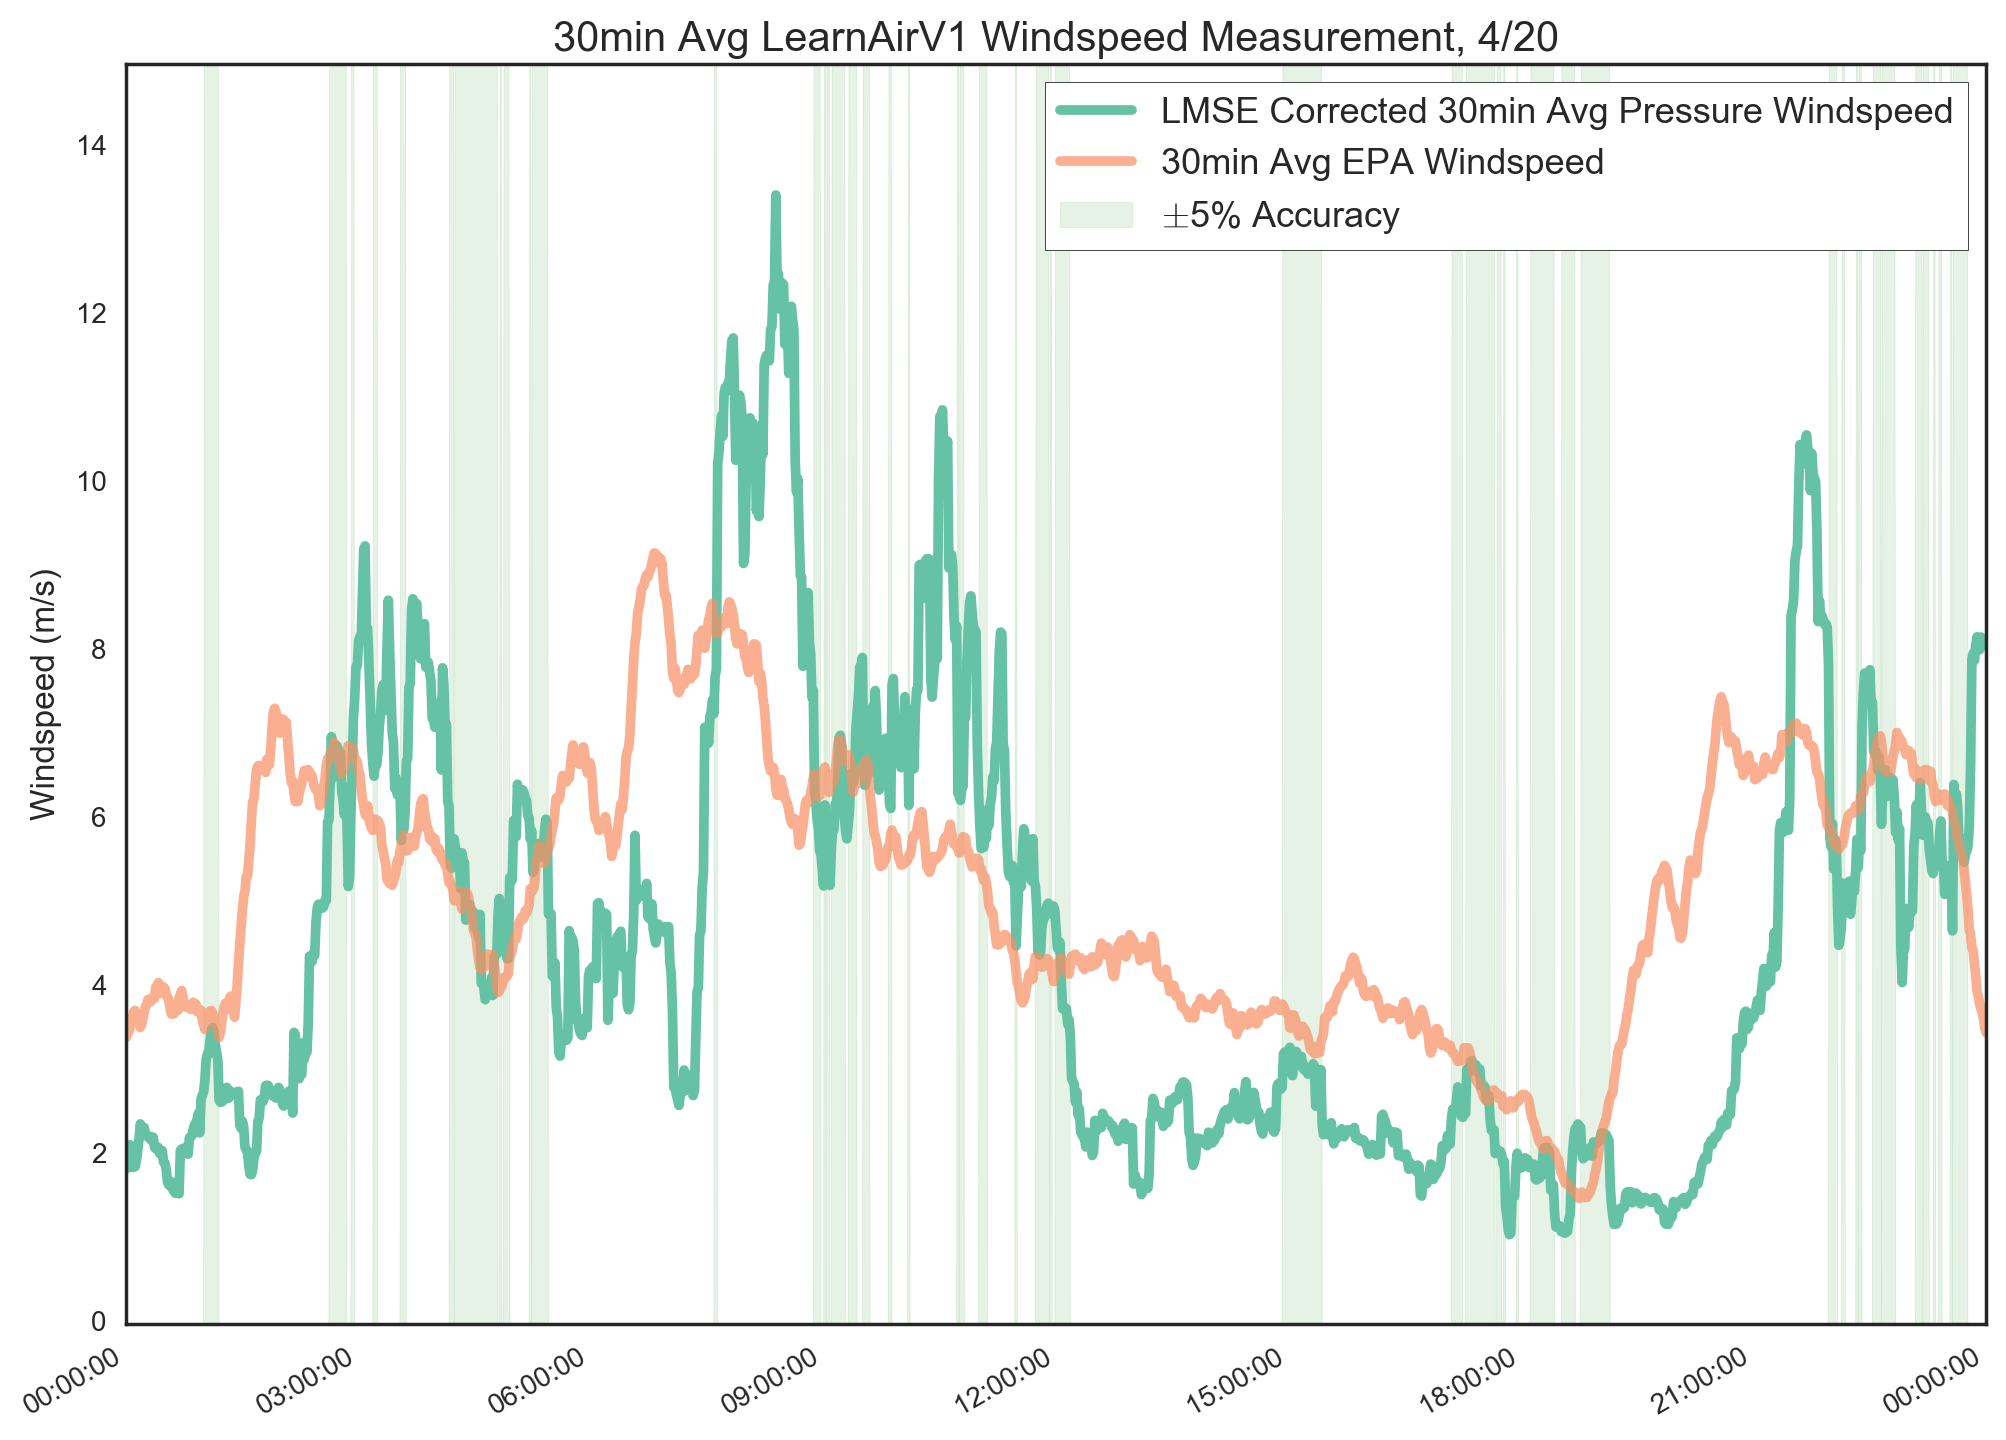
\includegraphics[width=\textwidth]{figs/ws_with_10_accuracy_zoomed}               
 	 \caption{Wind Speed Measurement with 10\% Accuracy, Zoomed}
  	\label{fig:ws_with_10_accuracy_zoomed}
\end{figure}

While the overall trend is there, there are some large discrepancies.  Based on our polar plots, it seems worthwhile to look at the differences between our measurement and the MassDEP measurement as a function of wind direction, as shown in Figure \ref{fig:ws_error_vs_wd}.  There are clear and interesting relationships between measurement inaccuracies and wind direction-- there are large differences in the readings when the wind approaches from ~60, 120, 210, 270 degrees, while 0, 90, 180, 260, and 320 degrees seem to match more closely.  This does not corroborate expectations exactly, given our polar plots (0 and 180 degrees having low error since they allow wind to pass, and 90 and 270 degrees having high error since they reject airflow).  These results suggest a more complicated relationship between direction and selectivity.  More rigorous testing is required to accurately characterize the directionality of this system.

\begin{figure}[htb]
 	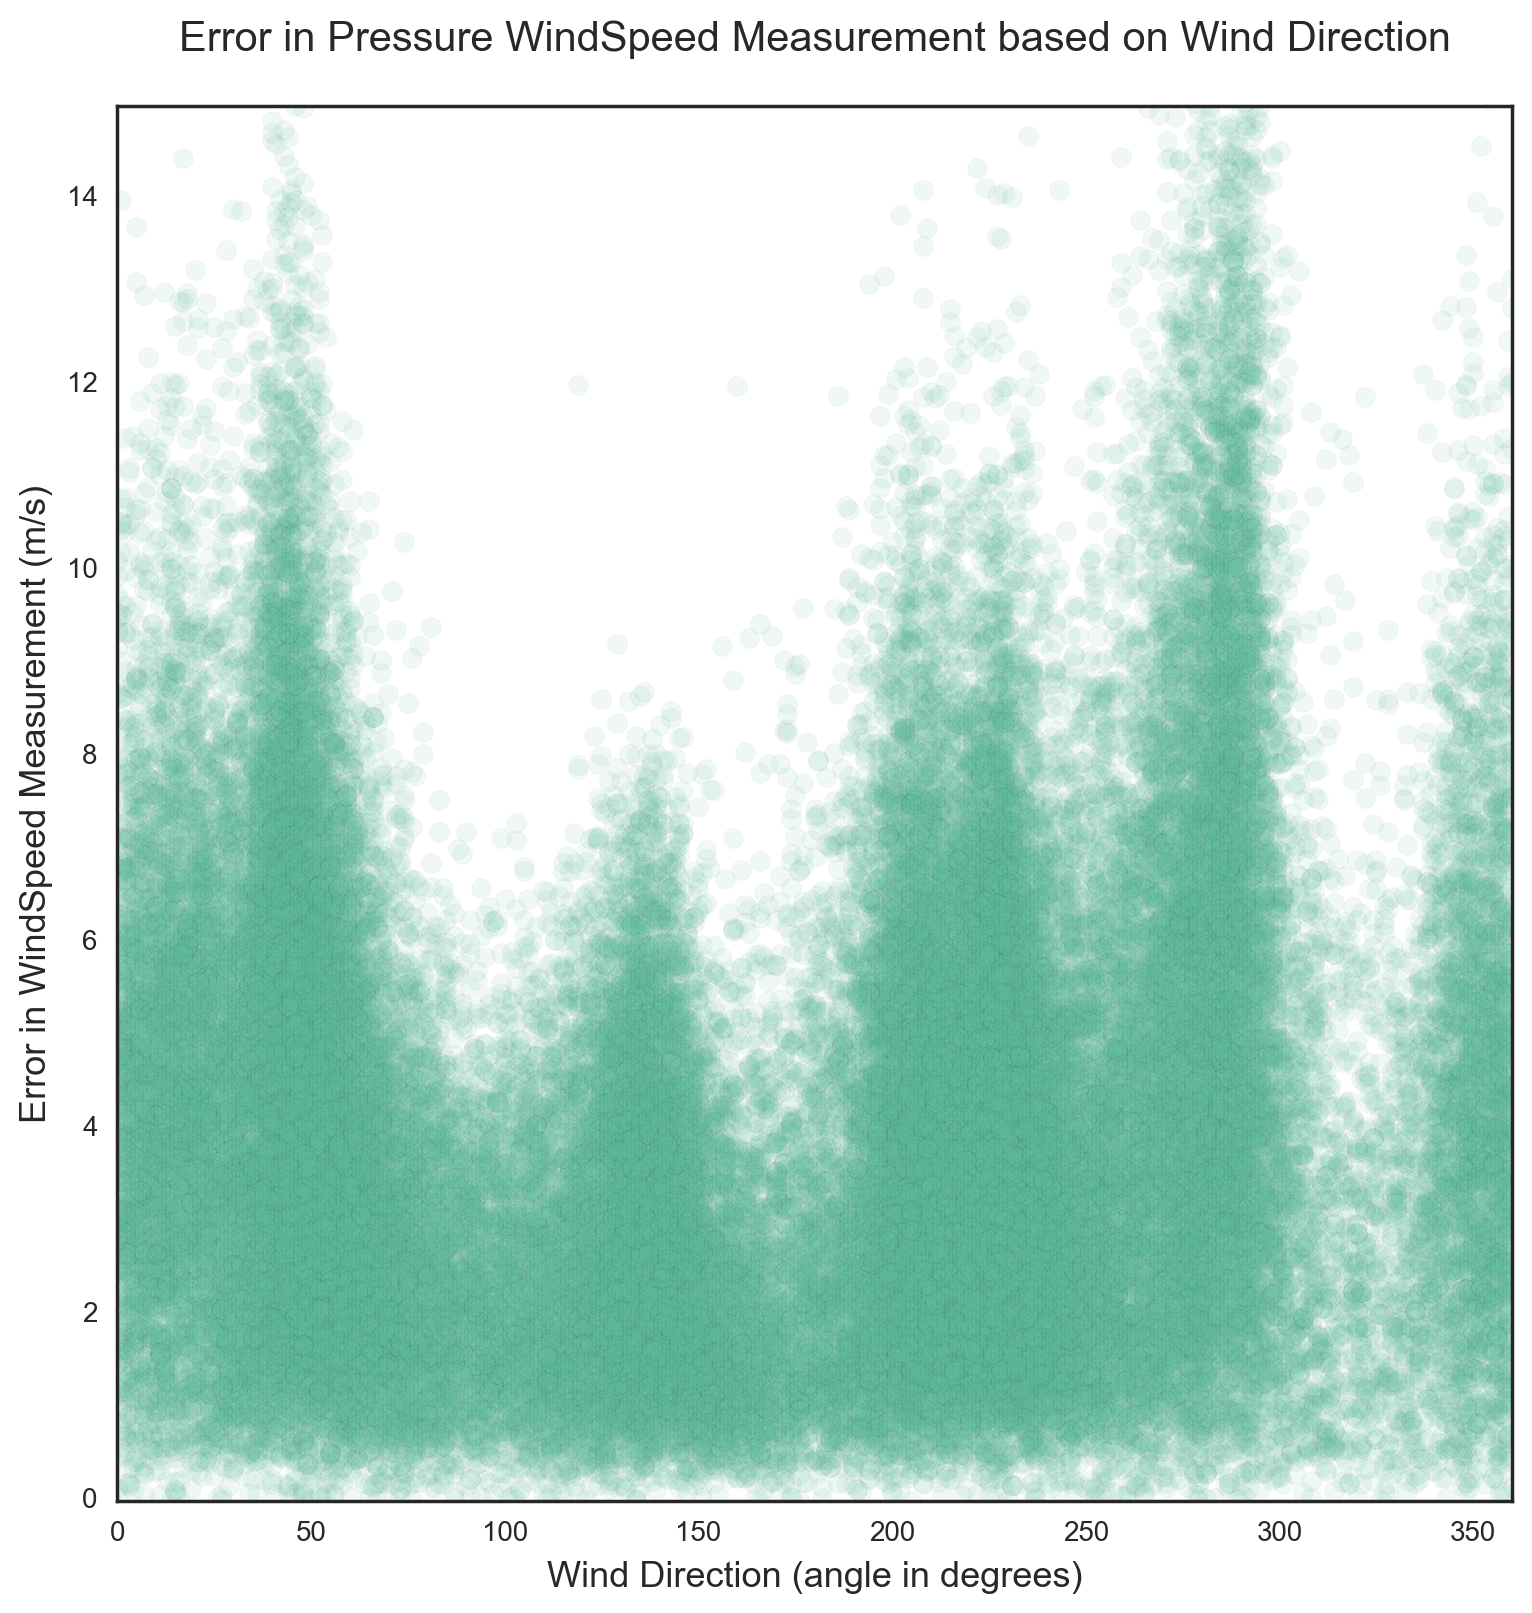
\includegraphics[width=\textwidth]{figs/ws_error_vs_wd}               
 	 \caption{Discrepency in Windspeed Measurement vs Wind Direction}
  	\label{fig:ws_error_vs_wd}
\end{figure}

The overall trends support the fact that our pressure sensor is measuring airflow in a correct and useful way.  Having a measure of airflow inside the slotted casing is good for tracking meaningful penetration of wind, regardless of direction.  This work suggests that pressure sensors have great potential to provide a low cost, small option for accurate wind sensing.  Future research is necessary to optimize sensor geometry, orthogonalize sensor axes, and characterize the effect of device geometry and turbulence on system linearity, in order to understand the wind sensing potential for this technology.  For this project, the pressure signal provides insight regarding near-field air flow that can be used as a training feature for our machine learning model.  More figures describing the wind data can be found in the Appendix.

\chapter{6. ChainAPI for Air Quality}

ChainAPI \cite{chainGit, chainPaper} is a hypermedia framework for the 'Web of Things'.  It provides a minimal layer of design principles on top of the HAL/JSON specification, to make data sharing and resource addressing simple.  It is extensible-- allowing anyone to define their own ontologies and connect their own data storage solutions in a distributed fashion-- and attempts to only rigorously define a thin, hyperlink layer that allows information to be easily discoverable and easily digestible by any user or service.

\begin{marginfigure}
 	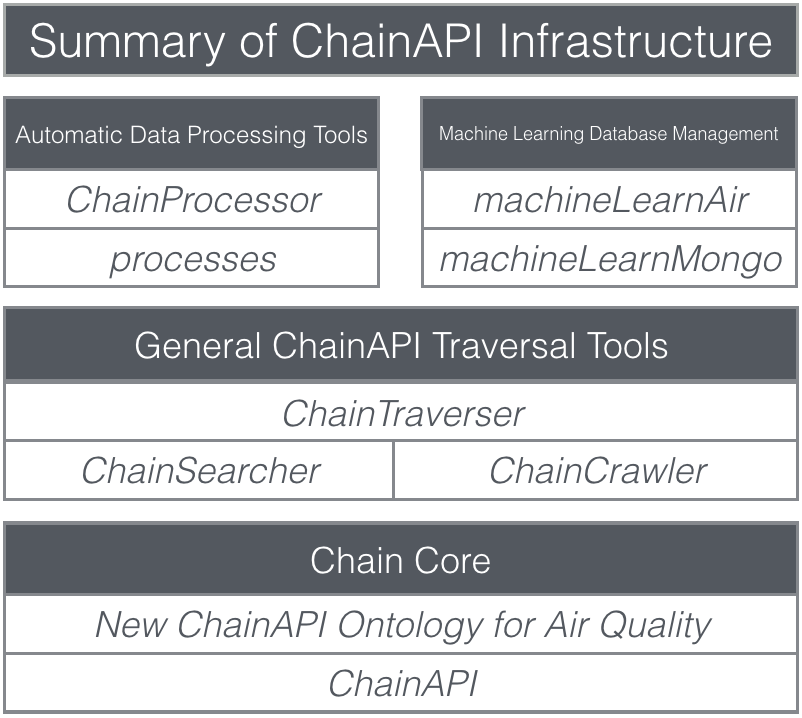
\includegraphics[width=\textwidth]{visuals/chainSummary}               
 	 \caption{Summary of New ChainAPI Infrastructure}
  	\label{fig:chain}
\end{marginfigure}

ChainAPI lends itself to the kinds of problems facing the air quality community.  It allows anyone, with any type of device, to store their data however they see fit, and still easily connect to a broader ecosystem.  It allows researchers to browse through the entire ecosystem like they would the internet.  It incentivizes contribution with a broader data ecosystem and interesting tools, while simultaneously lowering the barrier to entry as much as possible.

In the Responsive Environments group at the MIT Media Lab, ChainAPI already forms the backbone of a large ecological sensor network installation called TidMarsh. \cite{tidmarsh}  It connects hundreds of sensors to a browsable, easy to use backend.  It provides a simple real-time data stream that developers have connected to for building virtual environments, data visualizations, audio compositions, and other novel tools for data interaction.  Besides addressing the core concerns of distributed, scalable, simple data-sharing, ChainAPI also stands as the backbone of several future-looking human interactions and interventions to help individuals live with, understand, internalize, and mediate large datasets.

The TidMarsh ChainAPI environment forms the basis of the ChainAPI Air Quality protocol.  To make it useful for air quality, the first step is to define an ontology that addresses the needs and concerns of the air quality community.  This ontology is significantly larger and more complex than the current ChainAPI ontology, catering specifically to concerns of stationary and mobile air quality sensing.  This includes shared resources that define sensor types and device types and relevant metadata, as well as Organizational and Fixed Site information so that larger groups like the EPA have an example resource that maps well to their current ontology.

While several interesting tools have been created on top of the core ChainAPI for interacting with live streams of known resources, there are no tools to automatically explore and interact with a data ecosystem that is dynamic and growing, or an ecosystem that has reached critical mass (i.e. one update stream becomes infeasible as a way of monitoring all resources).  These are features we would expect from a true, distributed 'Web of Things' solution, and are of particular concern for an air quality installation designed to support deployments ranging from the EPA to small citizen groups.  These features also lay the groundwork for scalable learning algorithms, that can search the network for nearby higher quality sensors and utilize their data.

In this thesis, we define a new ontology for ChainAPI to adapt it to the air quality space.  After creating a development environment that takes advantage of this ontology, we created several tools to enable scalable interaction and advanced learning on this dataset.  These tools-- chainCrawler, chainSearcher, chainTraverser, and chainProcessor-- form a backbone of extensible, powerful options for resource discovery, automatic and transparent cross-organization dataset creation and processing, as well as scalable, advanced machine learning techniques.  It encourages programmatic data processing that can scale and is easily trackable.  It also encourages a separation of concerns-- so the best-in-class raw data collection and the best-in-class pre-processing algorithms can both exist transparently and be applied broadly, instead of siloed researchers batch processing and scrubbing data with opaque techniques before any data is shared.

At it's most advanced, these tools provide a simple way to find and compare co-located sensors of similar type but disparate quality, easily access the conditions under which those measurements occurred, and apply any user-defined algorithm.  This is all scaffolded in such a way that the underlying algorithm or model can simply and automatically update as more data is added to the network.    


\section{A New Ontology for Air Quality}

The first major step in adapting ChainAPI for air quality networks is to define a new ontology.  The basic outline is as follows:

\begin{quote}
\textit{Organizations have Deployments.  Deployments have Fixed Sites and Mobile Devices.  Both Fixed Sites and Mobile Devices have an extensible API datastore for weather conditions, etc. (corresponding to their location) associated with them.  Fixed Sites have (non-Mobile) Devices.  Devices each are associated with a particular Device Type (make and model), and each Device has a collection of Sensors (individual data streams).  Sensors are associated with a particular Sensor Type, and have a collection of SensorData.}
\end{quote}

There are other resources and details, which are outlined in the full documentation below.  Some data (like SensorData, CalibrationData, and APIData) have an associated storage resource that contains general, important information about the collection of data (like what it's measuring, which API it is calling, etc).  LocationData, on the other hand, requires no metadata, and thus does not require a storage resource.  'Type' resources are useful for quickly identifying resources of the same type, and centralizing information about how to handle that type.  

One interesting example of the utility of centralized resource types is that manufacturers could potentially oversee their device and sensor types-- updating metadata and associated calibration algorithms.  A new user to the ChainAPI system could then simply link their sensor resource to the correct type, and an automated crawler could pull the most recent, manufacturer-specified calibrations and apply them automatically to the new user's data.  It could check the conditions under which a measurement was made automatically, and warn the user if the sensor is out of normal operating ranges.  Additionally, the manufacturer could store sensor service information in their sensor type, and have an automated crawler that looks for sensors of that type, checks their serial numbers, and notifies the contact person associated with a resource if their sensor is in need of recalibration.  
   
In general, the principle behind data storage in ChainAPI is to create many 'virtual sensors' to represent one real one.  We encourage users to store raw data in Chain, and after processing it, post the processed data to a parallel 'virtual sensor' that has a name that indicates it comes from the same physical sensor, but has new units or is a new metric. 

A few minutiae are important for interoperability.  Timestamps are stored using ISO8601 standards (timezone aware UTC)-- all python code and scripts will accept (and only accept) one of the major timezone-specified string formats.  Timed/averaged measurements are stored with a 'start time' and a 'duration'.

\begin{lstlisting}[style=codedef]
@@Organization@@
	
	%\textit{An installation of ChainAPI maintained and curated by an Organization.}%

	@@name@@(string) - the name of the organization.
	@@url@@(string) - the website URL associated with the organization.
	@@ch:deployments@@ (related resource) - a collection of deployments associated with the organization.
	@@ch:contacts@@ (related resource) - a collection of contacts associated with the organization.

\end{lstlisting}

\begin{lstlisting}[style=codedef]
@@Deployment@@
	
	%\textit{A particular project owned by an organization, usually with several to hundreds of mobile sensors and/or fixed sites.}%

	@@name@@(string) - the name of the deployment.
	@@geoLocation@@(elevation, latitude, longitude)  - a location to associate with the deployment; usually, the city where the deployment is based.
	@@ch:organization@@ (related resource) - the parent organization.
	@@ch:sites@@ (related resource) - a collection of fixed sites associated with the deployment.
	@@ch:devices@@ (related resource) - a collection of mobile devices associated with the deployment.
	@@ch:contacts@@ (related resource) - a collection of contacts in charge of the deployment.

\end{lstlisting}

\begin{lstlisting}[style=codedef]
@@Fixed Site@@
	
	%\textit{An immovable location where several devices are co-located.}%

	@@name@@(string) - the name/identifier of the site.
	@@url@@(string) - a website URL reference with extra documentation about the site.
	@@geoLocation@@(elevation, latitude, longitude)  - the fixed coordinates/elevation of the site.
	@@ch:deployment@@ (related resource) - the parent deployment.
	@@ch:devices@@ (related resource) - a collection of devices located at the fixed site.
	@@ch:calibration_datastores@@ (related resource) - a collection of calibration datastores associated with the site.
	@@ch:api_datastores@@ (related resource) - a collection of API datastores associated with the site location.	
	@@ch:contacts@@ (related resource) - a collection of contacts in charge of site maintenance.

\end{lstlisting}

\begin{lstlisting}[style=codedef]
@@Device@@
	
	%\textit{A manufactured object that houses a collection of sensors.  If it is mobile, its proper parent is a deployment.  If it is}%
	%\textit{stationary, its proper parent is a fixed site.}%

	@@unique_name@@(string) - a unique identifier for the device.
	@@serial_no@@(string) - the manufacturer's unique identifier for the device.
	@@deploy_date@@(ISO8601 timestamp) - the date the device was put in the field.	
	@@manufacture_date@@(ISO8601 timestamp) - the date the device was manufactured.
	@@description@@(string) - extra, descriptive data pertaining to this device.
	@@ch:device_type@@ (related resource) - general device information for this make/model device.
	@@ch:site@@ (related resource) - the parent site, if a fixed device.
	@@ch:deployment@@ (related resource) - the parent deployment, if a mobile device.
	@@ch:locationDataHistory@@ (related resource) - a collection of timestamped location data, if a mobile device.
	@@ch:api_datastores@@ (related resource) - a collection of API datastores associated with the device's timestamped locationData.
	@@ch:contacts@@ (related resource) - a collection of contacts in charge of the device.
	
\end{lstlisting}

\begin{lstlisting}[style=codedef]
@@Device Type@@
	
	%\textit{A collection of useful data pertaining to several devices of the same make and model.}%

	@@manufacturer@@(string) - the name of the device manufacturer.
	@@model@@(string) - the name/number of the device model.
	@@revision@@(string) - the hardware revision of the device.
	@@datasheet_url@@(string) - the website URL associated with the most current datasheet.
	@@description@@(string) - extra, descriptive data pertaining to this device type.
	@@ch:devices@@ (related resource) - a collection of all devices of this type.

\end{lstlisting}

\begin{lstlisting}[style=codedef]
@@Sensor@@
	
	%\textit{An object that captures a single channel of timestamped data.  There maybe multiple sensors in a device. }%

	@@metric@@(string) - a label for the measured quantity (i.e. 'O3', 'CO', 'NO2').
	@@unit@@(string) - the units of the measurement (i.e. 'ppb', 'ug/m3')
	@@ch:sensor_type@@ (related resource) - general sensor information for this make/model sensor.
	@@dataType@@(string) - the datatype stored by the sensor (float).
	@@value@@(float) - the most recent reading from the sensor.	
	@@updated@@(ISO8601 timestamp) - the timestamp of the most recent reading from the sensor.
	@@ch:dataHistory@@ (related resource) - the collection of timestamped data from this sensor.
	@@ch:device@@ (related resource) - the parent device.

\end{lstlisting}

\begin{lstlisting}[style=codedef]
@@Sensor Type@@
	
	%\textit{A collection of useful data pertaining to several sensors of the same make and model.}%

	@@manufacturer@@(string) - the name of the sensor manufacturer.
	@@model@@(string) - the name/number of the sensor model.
	@@revision@@(string) - the hardware revision of the sensor.
	@@datasheet_url@@(string) - the website URL associated with the most current datasheet.
	@@description@@(string) - extra, descriptive data pertaining to this sensor type.
	@@retail_cost@@(float) - rough estimate of sensor cost, for future 'value' comparisons.
	@@learn_priority@@(int) - an indication of sensor trustworthiness.  This can be used so lower ranking sensors will learn from higher ranking ones automatically.
	@@service_interval_days@@(float) - number of days between recommended servicing.
	@@sensor_topology@@(string) - a description of device operating principles (i.e. 'BAM', 'electrochemical')
	@@ch:sensors@@ (related resource) - a collection of all sensors of this type.

\end{lstlisting}

\begin{lstlisting}[style=codedef]
@@Sensor Data@@
	
	%\textit{The raw data associated with a sensor.}%

	@@dataType@@(string) - the datatype of the raw data (float).
	@@totalCount@@(int) - total number of saved datapoints, or the number returned on this page if the dataset is large.
	@@data@@ (list) - a collection of data objects, each with a 'value' (float) and a 'timestamp' (ISO8601 timestamp)

\end{lstlisting}

\begin{lstlisting}[style=codedef]
@@API DataStore@@
	
	%\textit{An object that captures a single channel of external API data.  There maybe multiple API Datastores associated with a}%
	%\textit{mobile device or a fixed site. }%	

	@@metric@@(string) - a label for the measured quantity (i.e. 'temp', 'humidity).
	@@unit@@(string) - the units of the measurement (i.e. 'Celcius', 'percent')
	@@metadata@@(string) - an extra text field for relevant metadata.
	@@ch:api_type@@ (related resource) - general information about the external API.
	@@dataType@@(string) - the datatype stored in this API datastore (float).
	@@value@@(float) - the most recent value from the API.	
	@@updated@@(ISO8601 timestamp) - the timestamp of the most recent API call.
	@@ch:dataHistory@@ (related resource) - the collection of data from this API.
	@@ch:site@@ (related resource) - the parent site if associated with a site.
	@@ch:device@@ (related resource) - the parent device if associated with a mobile device.

\end{lstlisting}

\begin{lstlisting}[style=codedef]
@@API Type@@
	
	%\textit{A collection of useful data pertaining to a given external API.}%

	@@api_name@@(string) - the name of the API.
	@@api_base_address@@(string) - the base API access URL.
	@@description@@(string) - extra, descriptive data pertaining to this API.
	@@ch:devices@@ (related resource) - a collection of all mobile devices that use this API.
	@@ch:sites@@ (related resource) - a collection of all fixed sites that use this API.

\end{lstlisting}

\begin{lstlisting}[style=codedef]
@@API Data@@
	
	%\textit{The raw data associated with an API Datastore.}%

	@@dataType@@(string) - the datatype of the raw data (float).
	@@totalCount@@(int) - total number of saved datapoints, or the number returned on this page if the dataset is large.
	@@data@@ (list) - a collection of data objects, each with a 'value' (float), a 'timestamp' (ISO8601 timestamp), the 'api_call' used to retrieve the data (string), the 'api_access_time' (ISO8601 timestamp) when the call was initiated, and the 'duration_sec' (int) that the API data is useful for (starting from 'timestamp').

\end{lstlisting}

\begin{lstlisting}[style=codedef]
@@Calibration DataStore@@
	
	%\textit{An object that captures a single channel of calibration data.  There maybe multiple calibration datastores associated with}%
	%\textit{a mobile device or a fixed site. }%	

	@@metric@@(string) - a label for the measured quantity (i.e. 'sensitivity', 'voltage_offset').
	@@unit@@(string) - the units of the measurement (i.e. 'ppb/nA', 'mV')
	@@metadata@@(string) - an extra text field for relevant metadata.
	@@dataType@@(string) - the datatype stored in this calibration datastore (float).
	@@value@@(float) - the most recent calibration value.	
	@@updated@@(ISO8601 timestamp) - the timestamp of the most recent calibration.
	@@ch:dataHistory@@ (related resource) - the collection of data from calibration datastore.
	@@ch:site@@ (related resource) - the parent site if associated with a site.
	@@ch:sensor@@ (related resource) - the parent sensor if associated with a mobile device.

\end{lstlisting}

\begin{lstlisting}[style=codedef]
@@Calibration Data@@
	
	%\textit{The raw data associated with a Calibration Datastore.}%

	@@dataType@@(string) - the datatype of the raw data (float).
	@@totalCount@@(int) - total number of saved datapoints, or the number returned on this page if the dataset is large.
	@@data@@ (list) - a collection of data objects, each with a 'value' (float), a 'timestamp' (ISO8601 timestamp), a 'description' (string), and a 'contact' (related resource).

\end{lstlisting}

\begin{lstlisting}[style=codedef]
@@Location Data@@
	
	%\textit{The raw data that forms a collection of timestamped location information for tracking a mobile device.}%

	@@latitude@@(float) - a latitude GPS coordinate.
	@@longitude@@(float) - a longitude GPS coordinate.
	@@elevation@@(float) - elevation in meters.
	@@timestamp@@(ISO8601 timestamp) - the timestamp associated with this location reading.
	@@ch:device@@ (related resource) - the parent device.

\end{lstlisting}

\begin{lstlisting}[style=codedef]
@@Contact@@
	
	%\textit{A person that is part of an organization, oversees/calibrates a deployment or site, or owns a device.}%

	@@first_name@@(string) - a contact's first name.
	@@last_name@@(string) - a contact's last name.
	@@phone@@(string) - a contact's phone number.
	@@email@@(string) - a contact's email address.
	@@ch:organization@@ (related resource) - a contact's organization.
	@@ch:deployments@@ (related resource) - a collection of deployments overseen by the contact.
	@@ch:devices@@ (related resource) - a collection of devices owned by the contact.
	@@ch:sites@@ (related resource) - a collection of sites overseen by the contact.
	@@ch:calibration_data@@ (related resource) - a collection of calibration logs measured by the contact.

\end{lstlisting}






\section{Traversing ChainAPI}

\subsection{chainCrawler - a web-crawler for ChainAPI}

Now that we've created an ontology for air quality, it's important to have the tools to interact with the data as new devices are added.  ChainCrawler is a tool for crawling through ChainAPI resource links and discovering new resources.  It works like a traditional web-crawler.  

ChainCrawler is highly optimized for speed and scale, using Google's CityHash to track the most recently visited resources so the crawler doesn't loop or backtrack.  It has the additional feature of tracking hash collisions as required, and can accept any power of 2 size hash table.  

ChainCrawler accepts an entry point URI, and picks a random, unexplored link to traverse from that resource.  If it reaches a dead end or has already visited all of a resource's links, it moves back through its recent history (# of URIs in history are definable) to look for unexplored resources.  If it runs out of history, it returns to the entry-point resource.  At this point, if every entry-point resource path has been visited, the cache is cleared and the process is started over.

ChainCrawler will return the URI(s) of chain resources based on search criteria.  It can filter on resource\_type (i.e. 'Site' or 'Device'), resource\_title (i.e. 'Site #1- Roxbury' or 'Device #2'), any arbitrary object attribute, or any combination of the above.

ChainCrawler can be used in several modes.  It can be run in a blocking manner, and simply return the URI of the first resource it finds.  It can be run as a separate thread, and pass URIs to another thread using python's 'Queue' library.  It can also be run in ZMQ push mode, in which case all URIs are pushed out over a ZMQ socket using push/pull (preferred method). In these threaded cases, chainCrawler will not stop crawling until forced.  It will not return duplicate resources for over a given, user-definable, refractory period (which can be set to infinite). 



\begin{lstlisting}[style=codedef]
@@chainCrawler.ChainCrawler@@(entry_point, cache_table_mask_length, track_search_depth, found_set_persistence, crawl_delay, filter_keywords)
	
	%\textit{Initialize a ChainCrawler Instance.}%

	@@entry_point@@ ( = 'http://learnair.media.mit.edu:8000') is the URI of the resource to start crawling.
	@@cache_table_mask_length@@ ( = 8) is the exponent used to define the hash mask for the hash table. (hash table size = 2^cache_table_mask_length)
	@@search_depth@@ ( = 5) is the number of URIs we store in history, in case we exhaust all links and have to back up.
	@@found_set_persistence@@ ( = 720) is the time, in minutes, that a crawler will remember a resource it has already seen, and will not re-push it to the user 
	@@crawl_delay@@ ( = 1000) is the time, in ms, in between calls to the server to access chain resources.
	@@filter_keywords@@ ( = ['next','previous']) is an array of link relationships we want to ignore while crawling.  For our data, 'next' and 'previous' are required.


@@chainCrawler.ChainCrawler.find@@(namespace, resource_type, plural_resource_type, resource_title, resource_extra)
	
	%\textit{Blocking crawl that will exit/return the URI of the first matching resource.}%

	@@namespace@@ ( = "") is the base URI that defines the ontological relationships.  Prepended to resource_types. 
	@@resource_type@@ ( = None) is an optional resource type search criteria that must match a given resource for it to be returned.
	@@plural_resource_type@@ ( = None) is a search criteria that should correspond the resource_type field. Plural types are automatically generated by looking at the singular resource_type and adding 's' and 'es', but for words that have strange pluralization, it is important to give the correct plural form. 
	@@resource_title@@ ( = None) is an optional resource title search criteria that must match a given resource for it to be returned.
	@@resource_extra@@ ( = None) is an optional dictionary of attribute:value pairs that must match a given resource for it to be returned.


@@chainCrawler.ChainCrawler.crawl_thread@@(q, namespace, resource_type, plural_resource_type, resource_title, resource_extra)
	
	%\textit{Similar to find, but this function spins up a background thread crawler that will push URIs of the matching resources}% 
	%\textit{onto the queue 'q'.}%

	@@q@@ ( = None) is the Queue object that URIs will be pushed to for other python threads to access. 


@@chainCrawler.ChainCrawler.crawl_zmq@@(socket, namespace, resource_type, plural_resource_type, resource_title, resource_extra)
	
	%\textit{Similar to find, but this function spins up a background thread crawler that will push URIs of the matching resources}%
	%\textit{over a PUSH/PULL ZMQ socket.}%

	@@socket@@ ( = 'tcp://127.0.0.1:5557') is the ZMQ PUSH/PULL socket that URIs will be pushed to for other programs to access. 

\end{lstlisting}



\begin{lstlisting}[style=code]
crawler = ChainCrawler('http://learnair.media.mit.edu:8000/', found_set_persistence=2, crawl_delay=500)
    
#--- Blocking Find ---#
    x = crawler.find(namespace='http://learnair.media.mit.edu:8000/rels/', resource_type='sensor', resource_extra={'sensor_type':'AlphasenseO3-A4'})
    print x

#--- Threaded Queue ---#
testQueue = Queue.Queue()
crawler.crawl_thread(q=testQueue, namespace='http://learnair.media.mit.edu:8000/rels/', resource_type='Device', resource_title='test004')
    
#caution: this main loop doesn't end
while True:
    uri = testQueue.get()
    print uri

time.sleep(5)

#--- ZMQ Socket Push on TCP://127.0.0.1:5557 ---#
crawler.crawl_zmq(namespace='http://learnair.media.mit.edu:8000/rels/', resource_title='Device #1')
\end{lstlisting}



\subsection{chainSearch - a breadth first search tool for ChainAPI}

ChainCrawler allows us to randomly crawl through the entire chain infrastructure looking for a specified resource or resource type.  While this is powerful, it is also important to have a generalized tool that allows us to search for closely associated resources-- for instance, locating the sensors that are part of a device if we only know the device's URI.  Crawling would be the wrong strategy in this case.  

Instead, we want to examine all resources linked directly from the device to see if any match our query, and then examine the child relationships of those resources, and so on.  Perhaps we \textit{only} want the resource if it is a direct child.  In these cases, chainSearch- a breadth first search tool that will search within a specified number of link relationships away from the entry resource- is the correct tool for the job.  Combined with chainCrawler, we now have tools to crawl and find any/all resources in ChainAPI, and then intelligently traverse local relationships within the ChainAPI ecosystem.      


\begin{lstlisting}[style=codedef]
@@chainCrawler.ChainSearch@@(entry_point, crawl_delay, filter_keywords)
	
	%\textit{Initialize a ChainSearch Instance.}%

	@@entry_point@@ ( = 'http://learnair.media.mit.edu:8000') is the URI of the resource to start crawling.
	@@crawl_delay@@ ( = 1000) is the time, in ms, in between calls to the server to access chain resources.
	@@filter_keywords@@ ( = ['next','previous']) is an array of link relationships we want to ignore while crawling.  For our data, 'next' and 'previous' are required.


@@chainCrawler.ChainSearch.find_degrees_all@@(namespace, resource_type, plural_resource_type, resource_title, degrees)
	
	%\textit{Blocking, exhaustive breadth first search of all resource 'degrees' degrees away from the entry point.  Returns a list}%
	%\textit{of all URIs within 'degrees' # of links from the current resource that match the search criteria.  Returns an empty list}%
	%\textit{if no resources match criteria.}%

	@@namespace@@ ( = "") is the base URI that defines the ontological relationships.  Prepended to resource_types. 
	@@resource_type@@ ( = None) is an optional resource type search criteria that must match a given resource for it to be returned.
	@@plural_resource_type@@ ( = None) is a search criteria that should correspond the resource_type field. Plural types are automatically generated by looking at the singular resource_type and adding 's' and 'es', but for words that have strange pluralization, it is important to give the correct plural form. 
	@@resource_title@@ ( = None) is an optional resource title search criteria that must match a given resource for it to be returned.
	@@degrees@@ ( = 1) is the number of degree relationships to exhaustively search from the entry point for a matching resource.


@@chainCrawler.ChainSearch.find_first@@(namespace, resource_type, plural_resource_type, resource_title, degrees)
	
	%\textit{Same as find\_degrees\_all, but this blocking breadth first search will immediately exit and return a resource upon}% 
	%\textit{finding the first match.  If it exhaustively searches within degrees, it returns an empty list.}%

	@@degrees@@ ( = 3) is the number of degree relationships to exhaustively search from the entry point for a matching resource.


@@chainCrawler.ChainSearch.find_create_link@@(namespace, resource_type, plural_resource_type, degrees)
	
	%\textit{Exhuastive breadth first search that returns the first matching create-form URI for a resource of type resource\_type.}% 

	@@degrees@@ ( = 1) is the number of degree relationships to exhaustively search from the creation link of type 'resource_type'.


@@chainCrawler.ChainSearch.reset_entrypoint@@(new_entrypoint)
	
	%\textit{Helper function to reset 'entry point' of a ChainSearch instance for easy re-use.}% 

	@@new_entrypoint@@ ( = 'http://learnair.media.mit.edu:8000') is a string matching the URI of the new starting point resource.

\end{lstlisting}



\begin{lstlisting}[style=code]
searcher = chainSearch.ChainSearch('http://learnair.media.mit.edu:8000/devices/10')

#-- Find Creation Link to Make a Sensor on this Device --#
resource_uri = searcher.find_create_link(namespace='http://learnair.media.mit.edu:8000/rels/', resource_type='sensor' )
print resource_uri

#-- Change Starting Point for Search --#
searcher.reset_entrypoint('http://learnair.media.mit.edu:8000/devices/?site_id=1')

#-- Find First Device with Name 'Device #3' within 4 Link Steps --# 
resource_uri = searcher.find_first(resource_title='Device #3', degrees=4)
print resource_uri

#-- Find All Devices within 2 Link Steps --#
list_of_resource_uris = searcher.find_degrees_all(resource_type='Device', degrees=2)
print list_of_resource_uris
\end{lstlisting}



\subsection{chainTraverser - a stateful spider for ChainAPI}

Normally we think of web spiders as simple crawlers.  chainTraverser is a Spider that comes with extra functionality.  ChainTraverser always 'sits' on top of an associated ChainAPI resource.  It takes advantage of chainCrawler and chainSearch in a natural way-- from its current resource, it can (1) crawl randomly to another resource of a certain type, (2) search and traverse basic link relationships, (3) search and traverse complicated, pre-defined link paths, and (4) move forward and backwards relative to where it has been. 

Besides moving through ChainAPI from one resource to another, chainTraverser provides many tools to interact with the ChainAPI resource it is associated with.  From the current resource, chainTraverser can add new child resources, or even add cascading child resources along a pre-defined link path.  It can also pull and push data to and from its resource.

For all air quality applications, this is the primary tool used to GET/POST data to ChainAPI, as well as to handle traversal tasks from the trivial (i.e. finding the temperature sensor belonging to a device) to the extensive (i.e. creating a multi-sensor, multi-device site given a target organization name and deployment).


\begin{lstlisting}[style=codedef]
@@chainTraversal.ChainTraversal@@(crawl_delay, entry_point, namespace)
	
	%\textit{Initialize a ChainTraversal Instance.}%

	@@crawl_delay@@ ( = 1000) is the time, in ms, in between calls to the server to access chain resources.
	@@entry_point@@ ( = 'http://learnair.media.mit.edu:8000') is the URI of the resource to start crawling.
	@@namespace@@ ( = 'http://learnair.media.mit.edu:8000/rels/') is the base URI that defines the ontological relationships.  Prepended to resource_types. 


@@chainTraversal.ChainTraversal.print_state@@()
	
	%\textit{prints the current state- the associated resource, the resource type, and the traversal history.}%
	

@@chainTraversal.ChainTraversal.back@@()
	
	%\textit{moves the traverser back to the previous node.}%


@@chainTraversal.ChainTraversal.forward@@()
	
	%\textit{moves the traverser forward to the next node, if we've moved back in the history.}%


@@chainTraversal.ChainTraversal.find_a_resource@@(resource, name)
	
	%\textit{Blocking crawl to a resource of type 'resource', specifically one titled 'name' if name is passed.  Upon}%
	%\textit{completion, chainTraversal is associated with this resource.}%

	@@resource@@ is the resource type the traverser will crawl for and then update its state to reflect.
	@@name@@ ( = None) is name or title of the resource query we are crawling to match. If left as None, the first resource of the correct type will be considered a match.
	

@@chainTraversal.ChainTraversal.add_a_resource@@(resource_type, post_data, plural_resource_type)
	
	%\textit{This adds a resource of resource\_type with attributes in post\_data, one link from the current traversal node.}%
	%\textit{This is safe to call if a resource already exists- it will return False if a matching resource is found. }%
	%\textit{ Otherwise, it will create the resource and return the server response.}%  

	@@resource_type@@ the type of resource to be created (i.e. 'Device', 'Sensor')
	@@post_data@@ the required data to create the corresponding resource_type
	@@plural_resource_type@@ ( = None) is a search criteria that should correspond the resource_type field. Plural types are automatically generated by looking at the singular resource_type and adding 's' and 'es', but for words that have strange pluralization, it is important to give the correct plural form. 
	

@@chainTraversal.ChainTraversal.move_to_resource@@(resource_type, name, plural_resource_type)
	
	%\textit{This is designed to move to a neighboring resource with a link relationship to the current traversal node. }%
	%\textit{If no matching resource is found with the shallow breadth first search, the traverser will not move and the }%
	%\textit{function will return False (successful traversal returns True).}%  

	@@resource_type@@ is the resource type the traverser will search for and then update its state to reflect.
	@@name@@ ( = None) is name or title of the resource query we are searching to match.
	@@plural_resource_type@@ ( = None) is a search criteria that should correspond the resource_type field. Plural types are automatically generated by looking at the singular resource_type and adding 's' and 'es', but for words that have strange pluralization, it is important to give the correct plural form. 


@@chainTraversal.ChainTraversal.add_and_move_to_resource@@(resource_type, post_data, plural_resource_type)
	
	%\textit{This is a combination of the previous two functions, to create and move to a resource.  It is safe to}%
	%\textit{call if a resource already exists- it will not overwrite it, it will simply move to it.}%


@@chainTraversal.ChainTraversal.find_and_move_path_exists@@(path_list)
	
	%\textit{This expects a list of dicts that will guide us through Chain API.  It will crawl to find the first resource,}%
	%\textit{and then move through the following items one link relationship at a time, if they exist, until settling on}%
	%\textit{the last node.  If the path is incorrectly specified, it will move as far down the path\_list as possible.}%

	@@path_list@@ a list of dicts specifying types and names of existing resources to traverse.  i.e.,[{'type':'organization', 'name':'testOrg Name'}, {'type':'deployment', 'name':'learnairNet'}, {'type':'device', 'name':'device1'}]


@@chainTraversal.ChainTraversal.find_and_move_path_create@@(path_list)
	
	%\textit{This expects a list of dicts that will guide us through Chain API.  It will crawl to find the first resource,}%
	%\textit{and then move through the following items one link relationship at a time, creating resources if they don't}%
	%\textit{exist, until settling on the last node.}%

	@@path_list@@ a list of dicts specifying types of resources and post_data to traverse and/or create.  i.e., [{'type':'organization', 'name':'testOrg Name'}, {'type':'deployment', 'post_data':{'name':'learnairNet'}}, {'type':'device', 'post_data':{'name':'device1'}}]


@@chainTraversal.ChainTraversal.add_data@@(post_data, resource_type)

	%\textit{This adds data to a sensor, calibration datastore, api datastore, etc. if the traverser is located at that node.}%
	%\textit{It will post data without checking for existing data, and may result in duplicate copies.  If this is undesirable, }%
	%\textit{use ChainTraversal.safe\_add\_data().}%  

	@@resource_type@@ ( = 'dataHistory') the type of data resource to be created.  For normal sensors, the appropriate resource_type is the default 'dataHistory'.
	@@post_data@@ any array of properly formatted data values to post


@@chainTraversal.ChainTraversal.safe_add_data@@(post_data, resource_type, max_empty_steps)

	%\textit{This adds data to a sensor, calibration datastore, api datastore, etc. if the traverser is located at that node.}%
	%\textit{It will first pull data at the node where it should be posting.  If data exists at matching timestamp to}%
	%\textit{post\_data, these data won't be uploaded/duplicated.}%  

	@@resource_type@@ ( = 'dataHistory') the type of data resource to be created.  For normal sensors, the appropriate resource_type is the default 'dataHistory'.
	@@post_data@@ any array of properly formated data values to post
	@@max_empty_steps@@ ( = 10) for pulling the comparison data from the sensor.  This is the number of empty pages in a row we must see before we assume we've reached the end of the data stored in Chain (there is no explicit indication of earliest/latest measurements, it must be assumed by traversal).


@@chainTraversal.ChainTraversal.get_all_data@@(max_empty_steps, resource_type)

	%\textit{This pulls all data from a sensor, calibration datastore, api datastore, etc. if the traverser is located at}%
	%\textit{that node.  It will return a timestamp sorted list of dicts with the relevant data.}%

	@@max_empty_steps@@ ( = 10) the number of empty pages in a row we must see before we assume we've reached the end of the data stored in Chain (there is no explicit indication of earliest/latest measurements, it must be assumed by traversal).
	@@resource_type@@ ( = 'dataHistory') the type of data resource to be pulled.  For normal sensors, the appropriate resource_type is the default 'dataHistory'.

\end{lstlisting}



\begin{lstlisting}[style=code]
traveler = ChainTraversal()
traveler.print_state()

#-- Standard Traversal --#
traveler.find_an_organization('ResEnv Test Organization #1')
traveler.move_to_resource('deployment', 'Test Deployment #2')
traveler.back() #back to organization
traveler.forward() #forward to deploymet
traveler.move_to_resource('device', 'testdevice001') #move to device
traveler.add_and_move_to_resource('sensor', {'metric':'COT','sensor_type':'alphasenseCOT','unit':'ppb'})
    
#-- Add Data to Current Sensor --#
traveler.print_state()
traveler.safe_add_data(
       [{'value':64.1,'timestamp':'2016-05-18 20:09:00+0000'},
        {'value':65.0,'timestamp':'2016-05-18 20:11:00+0000'},
        {'value':62.2,'timestamp':'2016-05-18 20:12:00+0000'},
        {'value':64.3,'timestamp':'2016-05-18 20:13:00+0000'},
        {'value':63.9,'timestamp':'2016-05-18 20:14:00+0000'},
        {'value':63.7,'timestamp':'2016-05-18 20:15:00+0000'} ])

#-- Path List Examples --#
find_and_move_path_exists([{'type':'organization', 'name':'testOrg Name'}, {'type':'deployment', 'name':'learnairNet'}, {'type':'device', 'name':'device1'])

find_and_move_path_create([{'type':'organization', 'name':'testOrg Name'}, {'type':'deployment', 'post_data':{'name':'learnairNet'}}, {'type':'device', 'post_data':{'name':'device1'}}])
\end{lstlisting}


\section{ChainAPI Tools for Scalable, Automatic Data Analysis}  

\subsection{chainExcelPush - easily add spreadsheet data to ChainAPI}

One important part of the ChainAPI infrastructure to drive its adoption are basic tools for data manipulation and uploading.  chainExcelPush is a simple, extensible tool that uses chainTraversal to make uploading excel files and csv files quick and painless.

chainExcelPush provides one prototype file and requires one command to use properly.  The prototype file must be edited to (1) provide the general path through ChainAPI to the device where you would like to push the data, and (2) provide a mapping between each excel column label and the device's sensor in ChainAPI where it should post.  Once this prototype function has been filled out, running the chainExcelPush script will prompt the user to select the path to their excel files, and the rest will happen automatically.

This is an example of a prototype function for the LearnAir V1 device.  By modifying this 'smart\_upload' function, it is easy to automate any excel upload to chainAPI:

\begin{lstlisting}[style=code]
def smart_upload(upload_array):
    #look at keys, figure out where these values should be stored in chain
    #call upload and actually upload values

    def switch(x):
        return {
            'humidity ( % raw)':{
                'device':{
                    'unique_name':'learnAirFixedV1',
                    'device_type':'learnAirFixedV1'},
                'sensor': {
                    'sensor_type':'SHT21',
                    'metric':'humidity_raw',
                    'unit':'raw'},
                                    },

            'light ( lx)':{
                'device':{
                    'unique_name':'learnAirFixedV1',
                    'device_type':'learnAirFixedV1'},
                'sensor': {
                    'sensor_type':'BH1730FVC',
                    'metric':'light',
                    'unit':'lux'},
                                    },

            'nitrogen dioxide ( kohm)': {
                'device':{
                    'unique_name':'learnAirFixedV1',
                    'device_type':'learnAirFixedV1'},
                'sensor': {
                    'sensor_type':'MICS4514',
                    'metric':'NO2_raw',
                    'unit':'kOhm'},
                                    },

            'alphas1_aux': {
                'device':{
                    'unique_name':'learnAirFixedV1',
                    'device_type':'learnAirFixedV1'},
                'sensor': {
                    'sensor_type':'AlphasenseO3-A4',
                    'metric':'O3_raw_aux',
                    'unit':'raw'},
                                    },


	            ...<many other mappings>...


            'sharpdust': {
                'device':{
                    'unique_name':'learnAirFixedV1',
                    'device_type':'learnAirFixedV1'},
                'sensor': {
                    'sensor_type':'GP2Y1010AU0F',
                    'metric':'PM25_raw',
                    'unit':'raw'},
                                    } 
        }.get(x.lower(), None)

    for key in upload_array.keys():
        learnair_data_upload(

                [{'type':'organization', 'name':'MIT Media Lab'},
                {'type':'deployment', 'post_data':{'name':'LearnAirTestDev'}},
                {'type':'site', 'post_data':{'name':'RoxburyEPA'}}],

                switch(key),
                upload_array[key])   
\end{lstlisting}

In this example, the key in the switch array describes the excel or csv column label, and the associated object defines the device and sensor where data should be uploaded.  The non-variable part of the path (describing the organization, deployment, and site) is given below, in a list form.  After describing this mapping, any files can be uploaded by simply running the script from the command line, which will initiate a search prompt for folders/paths to relevant excel files:

\begin{lstlisting}[style=code]
>> ./chainExcelPush.py
\end{lstlisting}

\subsection{chainProcessor - scalable, automatic learning for ChainAPI ecosystems}

The previous tools for ChainAPI allow us to easily navigate ChainAPI and perform basic data manipulations with resources and data.  These tools come together in a more advanced tool-kit with chainProcessor-- a set of classes designed to scaffold and promote scalable ChainAPI algorithms.  ChainProcessor crawls through chain, pulls out any data associated with a given type of sensor, and provides an easy interface for scientists and data analysts to: (1) write simple raw data processing functions, (2) write more sophisticated calibration algorithms, and/or (3) write highly sophisticated, auto-updating, predictive machine learning algorithms.  In all of these cases, 'virtual sensors' representing processed data, calibrated data, or predicted data are posted back into ChainAPI alongside the original sensor stream.

The cornerstones of chainProcessor are the chainProcessor routine and the 'processes' folder, which has a prototype process example file.  The processes folder contains files that must be labeled with the name of a corresponding ChainAPI Sensor Type (i.e. 'AlphaSenseO3-A4.py').  The chainProcessor routine automatically pulls the process names from the processes folder and crawls ChainAPI for the sensor types that match a defined process.  When a resource is found, it queries the process file to see if additional local data is required for the data processing step, and then mediates dataflow to and from the process.  A prototypical process file for an SHT21 temperature sensor is shown below:


\begin{lstlisting}[style=code]
#SHT21Temperture.py

#every process must have required_aux_data and process_data routines
#every process should have its own dispatcher and processing functions 
#called from the dispatcher

import numpy as np
from .. import machineLearnDatastore

def dispatcher(metric, unit):
    #this tells which extra data are required and which functions to use
    #to process a given metric/unit combination for this sensor type
    
    return {
        'temperature_raw': { 'raw': {
            'function': raw_to_temp
            }},
        'temperature': { 'celcius':{
            'extra_data': ['humidity_corrected', 'light_corrected'],
            'function': temp_to_learned_temp
            }}

            }.get(metric, None)[unit]


#all functions should return [sensor_type, metric, unit, data_to_post]

def raw_to_temp(data):
    #processes raw SHT21 readings to accurate temperature using datasheet
    #equation posts to a 'SHT21Temperature' sensor measuring 'temperature'
    #in 'celcius' units on the same device as the 'raw' SHT21 temp. data
    
    for data_element in data:
        data_element['value'] =  -50.0 + 175.72 * (data_element['value'] * 10 / (2**(16) ) )
    
    return('SHT21Temperature', 'temperature', 'celcius', data)


def temp_to_learned_temp(data):
    #passes us 'humidity_corrected' and 'light_corrected' data from the
    #same device if it exists, to use for a more advanced calibration 
    #that accounts for humidity/light effects

    for data_element, humidity in zip(data['main'], data['humidity_corrected']):
        data_element['value'] =  -50.0 + 175.72 * (data_element['value'] * 10 / (2**(16) - 0.05 * humidity['value'])

    return('SHT21Temperature', 'temperature', 'celcius_learned', data['main'])


#---- DO NOT EDIT THESE FUNCTIONS ----#

def required_aux_data(metric, unit):
    #logic for extra data required by this module: for instance, if we
    #have an alphasense NO2-A4 sensor, if we have a raw working electrode
    #data we also need raw aux electrode data and perhaps raw temp data to
    #make sense of the reading and create a virtual sensor.  This returns
    #a list of required secondary data for the sensor_type of this file,
    #and the metric/unit of that type, so that the main process routine
    #can traverse, find that extra data, and pass it back to process_data
    try:
        return dispatcher(metric, unit)['extra_data']
    except:
        return None


def process_data(data, metric, unit):
    #call logic - depending on metric/unit, call subprocess
    #return processed data and metric/unit to post
    try:
        return dispatcher(metric, unit)['function'](data)
    except:
        return None

#---- DO NOT EDIT THESE FUNCTIONS ----#
\end{lstlisting}

In this function, the user edits the dispatcher and writes data processing functions.  The dispatcher defines two key relationships for a given sensor type, metric, and unit combination-- it defines auxiliary data, and it defines the name of the function in the process file that will accept, modify, and return a processed version of that data.  The auxiliary data is assumed to be local data on the device or at the site-- for instance, local temperature or humidity readings, or auxiliary electrode readings, that are required to properly calibrate a sensor stream.  For more advanced algorithms and machine learning techniques that require extra information and extra state beyond what is available from the sensor and its neighbors, support functions discussed below can be integrated into these processes to enable them to learn and update their model over time.  These scripts are user-definable and can be run on any chainAPI instance.

Thus, the main process routine has four main jobs.  First, it crawls and finds sensor data that matches the defined process.  Then it looks at the process dispatcher, and determines which extra local data the process needs.  It pulls all of this data from the resource, and stamps every datapoint with latitude and longitude information based on its timestamp, and the available location data (for mobile devices) or the GPS coordinates (for fixed devices and sites).  This data (indexed on timestamp, latitude, and longitude) is used to call the relevant process function.  The main process then waits for a return list of post\_data for a virtual sensor-- the sensor\_type, metric, unit, and an array of data.  This return list is posted to ChainAPI at the parent device of the original sensor.     

This structure is already interesting and useful- instead of pre-processing data and pushing it after a set calibration or after running opaque, complicated data processing, this model allows (1) easy updating of calibration and data processing algorithms as they get better or more refined, (2) more transparent sharing of raw data, processed data, and processing routines, and (3) open the opportunity for manufacturers to track their own hardware, flag anomalies, qualify sensors as they age, and own/improve/update the routines used for calibrating their sensors.   

While this is interesting, the end goal is to enable sophisticated machine learning with this technique.  To that end, a support module called machineLearnDatastore comes into play.

For the purposes of machine learning, we divide our sensors up into 'conditions' and 'measures'.  This is an arbitrary distinction, but generally speaking 'conditions' are reliable, trusted, simple measurements and API calls that will be used to predict the accuracy of more complex and less reliable air quality 'measures'.  It is possible, using this technique, to easily add any 'measure' to a 'conditions' array when desired.

machineLearnMongo is a helper class that can be used in any process.  It creates a MongoDB database, with one consolidated collection for all 'conditions' (things like temperature and humidity), and one independent collection for each 'measure' (things like O3 readings from AlphaSense O3-A4 sensors).  MachineLearnMongo takes care of saving all of the data whenever a new update comes in, and consolidating conditions into one table.  All data in machineLearnMongo are indexed by timestamp, latitude, and longitude.  

The most important part of machineLearnMongo is the 'get\_values\_in\_range' and 'create\_ml\_array' functions.  The first of these allows searching any collection for values within a given time and location window.  The closest values to the ideal time and/or location are returned if multiple values fall within the window.  The second function automatically pulls all data from a 'measure' collection, and finds all the associated 'conditions' (and additional specified measures) that were measured within the specified time/location window of each measure datapoint.  This one simple command will examine all measurements that have been crawled by chainProcessor, match all data that was coincident, and return a full array of features that can be used to predict and train a machine learning model for the specified 'measures' array.  

At the moment, the user must define which other sensor types a given sensor should learn from.  However, fields are included in this ontology to automate that process-- giving a rank to each sensor, so that lower quality sensors can automatically learn from any higher quality reference.  This field can be entered manually (by an independent and trustworthy testing organization), or programatically by an algorithm that tracks sensor quality and revises rankings accordingly.

Additionally, the get\_values\_in\_range function returns the actual distance and delay between two measurements so it may be accounted for when training on the comparison data.  As the dataset grows, it is possible to automatically and rigorously converge on the useful range of distance and time offsets (simply by using this information as another feature in the machine learning feature vector).

\begin{lstlisting}[style=codedef]
@@machineLearnDatastore.machineLearnMongo@@(db)
	
	%\textit{Initialize a MongoDB database handler instance.  This is optimized for machine learning, and everything is indexed by}%
	%\textit{timestamp, latitude, and longitude.}%

	@@db@@ ( = 'learnair') is the name of the Mongo database
	

@@machineLearnDatastore.machineLearnMongo.create_indexed_collection@@(collection_name)
	
	%\textit{Initialize a MongoDB collection in our database, indexed by timestamp, latitude, and longitude.  This is used to initialize}%
	%\textit{collections of 'measures'.}%

	@@collection_name@@ is the name of the new Mongo collection that will be created.
	

@@machineLearnDatastore.machineLearnMongo.create_conditions_collection@@(collection_name)
	
	%\textit{Initialize a MongoDB collection in our database, indexed by timestamp, latitude, and longitude.  This is used to initialize}%
 	%\textit{the database's collection of 'conditions'.  As new conditions are added, only }%


@@machineLearnDatastore.machineLearnMongo.add_data_to_collection@@(collection_name, data)
	
	%\textit{Add data to one of the Mongo 'measures' collections.}%

	@@collection_name@@ is the name of the Mongo collection we'd like to add data to.
	@@data@@ is the data to be added.  Data should be formed as [ {'timestamp':x, 'lat':y, 'lon':z, 'fieldtoadd':xyz}, {'timestamp':x, 'lat':y,'lon':z, 'fieldtoadd':xyz} ].
	

@@machineLearnDatastore.machineLearnMongo.add_conditions@@(data)
	
	%\textit{Add data to one the 'conditions' collections.}%

	@@data@@ is the data to be added.  Data should be formed as [ {'timestamp':x, 'lat':y, 'lon':z, 'fieldtoadd':xyz}, {'timestamp':x, 'lat':y,'lon':z, 'fieldtoadd':xyz} ].


@@machineLearnDatastore.machineLearnMongo.print_collection@@(collection_name)
	
	%\textit{Print collection\_name collection to assess data and structure.}%

	@@collection_name@@ is the name of the Mongo collection we'd like to print.


@@machineLearnDatastore.machineLearnMongo.print_conditions@@()
	
	%\textit{Print 'conditions' collection to assess data and structure.}%


@@machineLearnDatastore.machineLearnMongo.get_collection_data@@(collection_name, query)
	
	%\textit{Access data from the 'collection\_name' collection.}%

	@@collection_name@@ is the name of the Mongo collection we'd like to query.
	@@query@@ (= {}) is the query to use on the collection.  If left blank, all documents in the collection will be returned.


@@machineLearnDatastore.machineLearnMongo.get_conditions_data@@(query)
	
	%\textit{Access data from the 'conditions' collection.}%

	@@query@@ (= {}) is the query to use on the collection.  If left blank, all documents in the collection will be returned.


@@machineLearnDatastore.machineLearnMongo.return_ml_array@@(collection_name, conditions, measure, extra_conditions, update_conditions_first, time_range, lat_lon_range, loc_then_time, return_diffs)
	
	%\textit{Creates and returns a machine learning useful array.  In summary, it takes the values from the}% 
	%\textit{collection\_name, finds conditions in the conditions array that are taken at similar timestamps/latitudes/ }% 	
	%\textit{longitudes, and combines them into an array where conditions can be used to predict measures. }%
	%\textit{This array is of the form:}%
	   [{'conditions':{'keya':val, 'keyb':val}, 'measures':{'keya':val, 'keyb':val}},
            {'conditions':{'keya':val, 'keyb':val}, 'measures':{'keya':val, 'keyb':val}},
            {'conditions':{'keya':val, 'keyb':val}, 'measures':{'keya':val, 'keyb':val}}]  
	%\textit{Specifically it adds the fields in 'measure' from the 'collection\_name' collection (and takes all of them if}%
	%\textit{none are specified), and pulls 'conditions' from the conditions collection (pulling all fields if none are}%
 	%\textit{specified) that match the timestamp, latitude, and longitude of the measures.  When there is a match-}%
	%\textit{ i.e., when we have conditions that line up with a measure- a new row in the returned machine learn}%
	%\textit{array is formed.  Instead of having to index an exact lat/lon/timestamp match (which is nearly impossible),}% 
	%\textit{this function takes a time\_range and a lat\_long\_range where it considers measurements coincident.}%
  	%\textit{If more than one condition value of the same type qualify as coincident, loc\_then\_time can be used}%
	%\textit{to set the more important feature (i.e. whether the closer value in time or the closer value in proximity}%
	%\textit{takes priority).  If multiple conditions entries are 'coincident' but have different fields, the full union}%
	%\textit{of fields will be returned.  Overlapping fields within these will prioritize the 'closer' condition.}% 

	@@collection_name@@ is the name of the Mongo 'measure' collection for which we'd like to apply machine learning.
	@@conditions@@ {= None) are the fields stored in the conditions array we'd like to add to our machine learning array.  If unspecified (None), all fields are used.
	@@measure@@ {= None) are the fields stored in the collection_name array we'd like to add to our machine learning array.  If unspecified (None), all fields are used.
	@@extra_conditions@@ {= None) is a dictionary of extra collections/fields that we'd like to add to our conditions array (for instance, if we want to add a cheap NO2 sensor 'measure' to our 'conditions' array to predict the accuracy of a cross-sensitive O3 sensor).  This dictionary should be of the form {collection_name:[field1, field2], collection_name:[field1, field2]}.
	@@update_conditions_first@@ {= True) will run through all indices in our conditions array (indexed by timestamp/lat/lon) and add API call data to each where it is missing, before constructing this array.
	@@time_range@@ {= 30) the time range, in seconds, for which two measurements are considered 'coincident'.
	@@lat_lon_range@@ {= 1) the range, in degrees, for which two latitude or longitude measurements are considered 'coincident'.
	@@loc_then_time@@ {= True) if two of the same value are coincident with the measure in collection_name, prioritize the one closer in distance instead the one closer in time if True.
	@@return_diffs@@ {= True) add metadata for the difference in lat/lon/time between the 'measure' collection and the 'conditions' into the conditions array (i.e. 'time_diff', 'lat_diff', 'lon_diff', 'distance')

	
@@machineLearnDatastore.machineLearnMongo.get_values_in_range@@(collection_name, timestamp, lat, lon, time_range, lat_lon_range, loc_then_time, return_diffs)

	%\textit{Return one document from collection\_name that is the closest fit to timestamp/lat/lon in the ranges}%
	%\textit{specified (within 30 seconds, 1 degree of lat and lon by default).  If there are no documents, return None.}%
	%\textit{time\_range, lat\_lon\_range, loc\_then\_time, and return\_diffs all operate the same with the same}%
	%\textit{defaults as return\_ml\_array above.}%
\end{lstlisting}


Instead of interacting directly with the machineLearnMongo class, the machineLearnAir class was created as an intermediary.  It provides a scaffolding for adaptive, scalable machine learning algorithms.  

MachineLearnAir is designed to manage a machineLearnMongo class, as well as typical machine learning algorithms that require a computationally intense 'training' phase.  When data is passed to a machineLearnAir instance, it is written to a machineLearnMongo database.  The class tracks when a training step was last run, and if enough new samples (more than update\_model\_with\_x\_new\_entries) have been added since the last update, the training step is triggered to run on all of the data stored in the machineLearnMongo instance managed by the class.  This training step then updates a Mongo representation of the machine learning model.

Regardless of whether the training step is called or not, data passed to the machineLearnAir instance will be passed to the main machine learning algorithm.  This step recalls the model trained in the previous step and apply it to the input data, returning processed data.  Both the model and the last\_updated state are saved, so stopping the process will not remove the most recent machine learning model.

Any user can add a new machine learning algorithm to the class simply by writing two functions-- an 'algorithm\_training' function, and an 'algorithm' function.  When passing data to the instance, simply giving the argument algorithm='algorithm' will use the newly added code.

These functions are scaffolded in the example below-- machine learning input data is pulled from the local machineLearnMongo collection, and the model (once trained in the training phase) should be stored with a model.post(<state>) command.  The main algorithm function can access that model using the model.get() command, and should return a list of processed data.

In short, this function manages all of the hard parts of machine learning.  Simply 'run' it on all data from a given sensor, and it will apply the latest machine learning model of that sensor to the data and return it.  Whenever it accumulates a large enough batch of new data, it triggers the '\_training' step that retrains the model using all available machine learning data.  It automatically recognizes its specified algorithms, so it is easy to add a new algorithm by simply writing the 'algorithm' function and the 'algorithm\_training' function as shown in the prototype file below. This makes it easily extensible for all types of new algorithms and techniques.
   

\begin{lstlisting}[style=code]
from machineLearnDatastore import *

learner = machineLearnAir(collection_name="AlphaSenseNO2" , update_model_with_x_new_entries=500)  

post_data = learner.run(input_data, algorithm='svm')
\end{lstlisting}

\begin{lstlisting}[style=code]
machineLearnAir.py

<...>

def svm_train(self, model):

	input_data = self.mongo.get_ml_array() #uses current collection

	<...training a ML model on input_data and store it in model_state...>

	model.post(model_state)


def svm(self, data, model):

	ml_model_state = model.get()

	<...apply the model to the data...>

	return processed_data


\end{lstlisting}


\section{Summary}

ChainAPI represents a unique and powerful solution to data sharing and data interaction for sensor networks.  It facilitates a scalable, distributed ecosystem while promoting easy interoperability and low barriers to entry.  

In this thesis, we've adapted the ChainAPI ecosystem to address the needs of air quality community.  This new ontology takes into consideration existing practices, as well as future needs of major research groups, citizen scientists, consumer product designers, and air quality equipment manufacturers.  The development implementation was built to run and interface with our learnAir hardware and stream data to/from a smartphone application.

On top of the ChainAPI solution, we've also added all of the new infrastructure explained in detail above.  We wrote these new tools \textit{(chainSearcher, chainCrawler, chainTraverser, chainProcessor, machineLearnAir, and machineLearnMongo)} that look towards a scalable, dynamic future for ChainAPI, as well as advanced functionality for scraping ChainAPI, running machine learning algorithms that constantly update as new data is added to the ecosystem, and reposting processed data to the system.  This scaffolding-- a hypermedia layer to connect the air quality data ecosystem supporting crawlers that run through the ecosystem processing data, updating their data processing models using that data, and posting their processed data back to the ecosystem to be further assessed-- is a novel topology for database design with interesting separation of concerns and transparency.

Besides the big picture ramifications of such a system, it allows us to accomplish our immediate goal-- (1) build a sensor that can post its data to chain, (2) easily scrape the database for nearby, coincident measurements of other sensors and ambient conditions, (3) run and update a machine learning script to predict the accuracy of that sensor's measurement, and (4) subscribe to a live feed of that processed data so we can display and update the live prediction of that sensor's reliabilty based on all of the latest ChainAPI data. 














%@@chainTraversal.ChainTraversal.find_a_deployment@@(name)
%@@chainTraversal.ChainTraversal.find_a_site@@(name)
%@@chainTraversal.ChainTraversal.find_an_organization@@(name)
%@@chainTraversal.ChainTraversal.find_a_device@@(name)
%
%	%\textit{Blocking crawl to an air quality resource of the type specified in the function name, specifically one}%
%	%\textit{titled 'name' if name is passed.  Upon completion, chainTraversal is associated with this resource.}%
%	%\textit{These are convenience functions that utilize ChainTraversal.find\_a\_resource().}%
%	

\chapter{7. Data Analysis and Machine Learning}

In the last two chapters we outlined the portable hardware that was built to measure air quality and push it up to ChainAPI.  We discussed our new backend infrastructure to support air quality data, as well as the tools that were created to allow automatic and extensible machine learning algorithms.  The final element of the system-- and the key element of this project-- is the evaluation of predictive machine learning algorithms in the air quality space.
 
For this test, we were able to co-locate six types of cheap air quality sensor next to EPA reference-level equipment for two months.  In most cases we collected minute-resolution data.  The testing occurred over the course of spring (with high variation in weather as we transitioned from the end of the cold/snowy season to the summer).   

This experimental design gives us the ability to take the difference between our cheap sensor signals and the EPA reference to generate an error signal.  Based on measurements from other sensors on the device in concert with data from external weather APIs, we can apply supervised learning techniques that attempt to predict the magnitude of the error for every reading.  

While there are many potential algorithms we could apply to this problem, for this experiment we simplified our error readings to a binary feature-- indicating whether the cheap sensor was in error or not, based on an appropriate tolerance around the ground truth value.  A logistic regression model-- commonly used for engineering failure prediction-- was selected to predict whether the sensor was in error, as well as assign a probability to this prediction.

<Summary of interesting take aways and results.>

\section{Test Conditions and Data Collection Summary}
 The learnAir V1 sensor was first installed on April 6th, 2016 and taken down on April 14th.  This preliminary test resulted in serious sensor corrosion and unuseable data.

The useful section of the co-location test ran from April 15th to June 13th (59 days).  During that time, several tests were performed.  In total we validated 8 different sensors representing 6 distinct sensor types over periods ranging from 21 to 59 days.  Our co-located test sets range from 1,431 samples of hourly data up to 85,739 samples of minute-resolved data.  


\begin{figure}[htb]
 	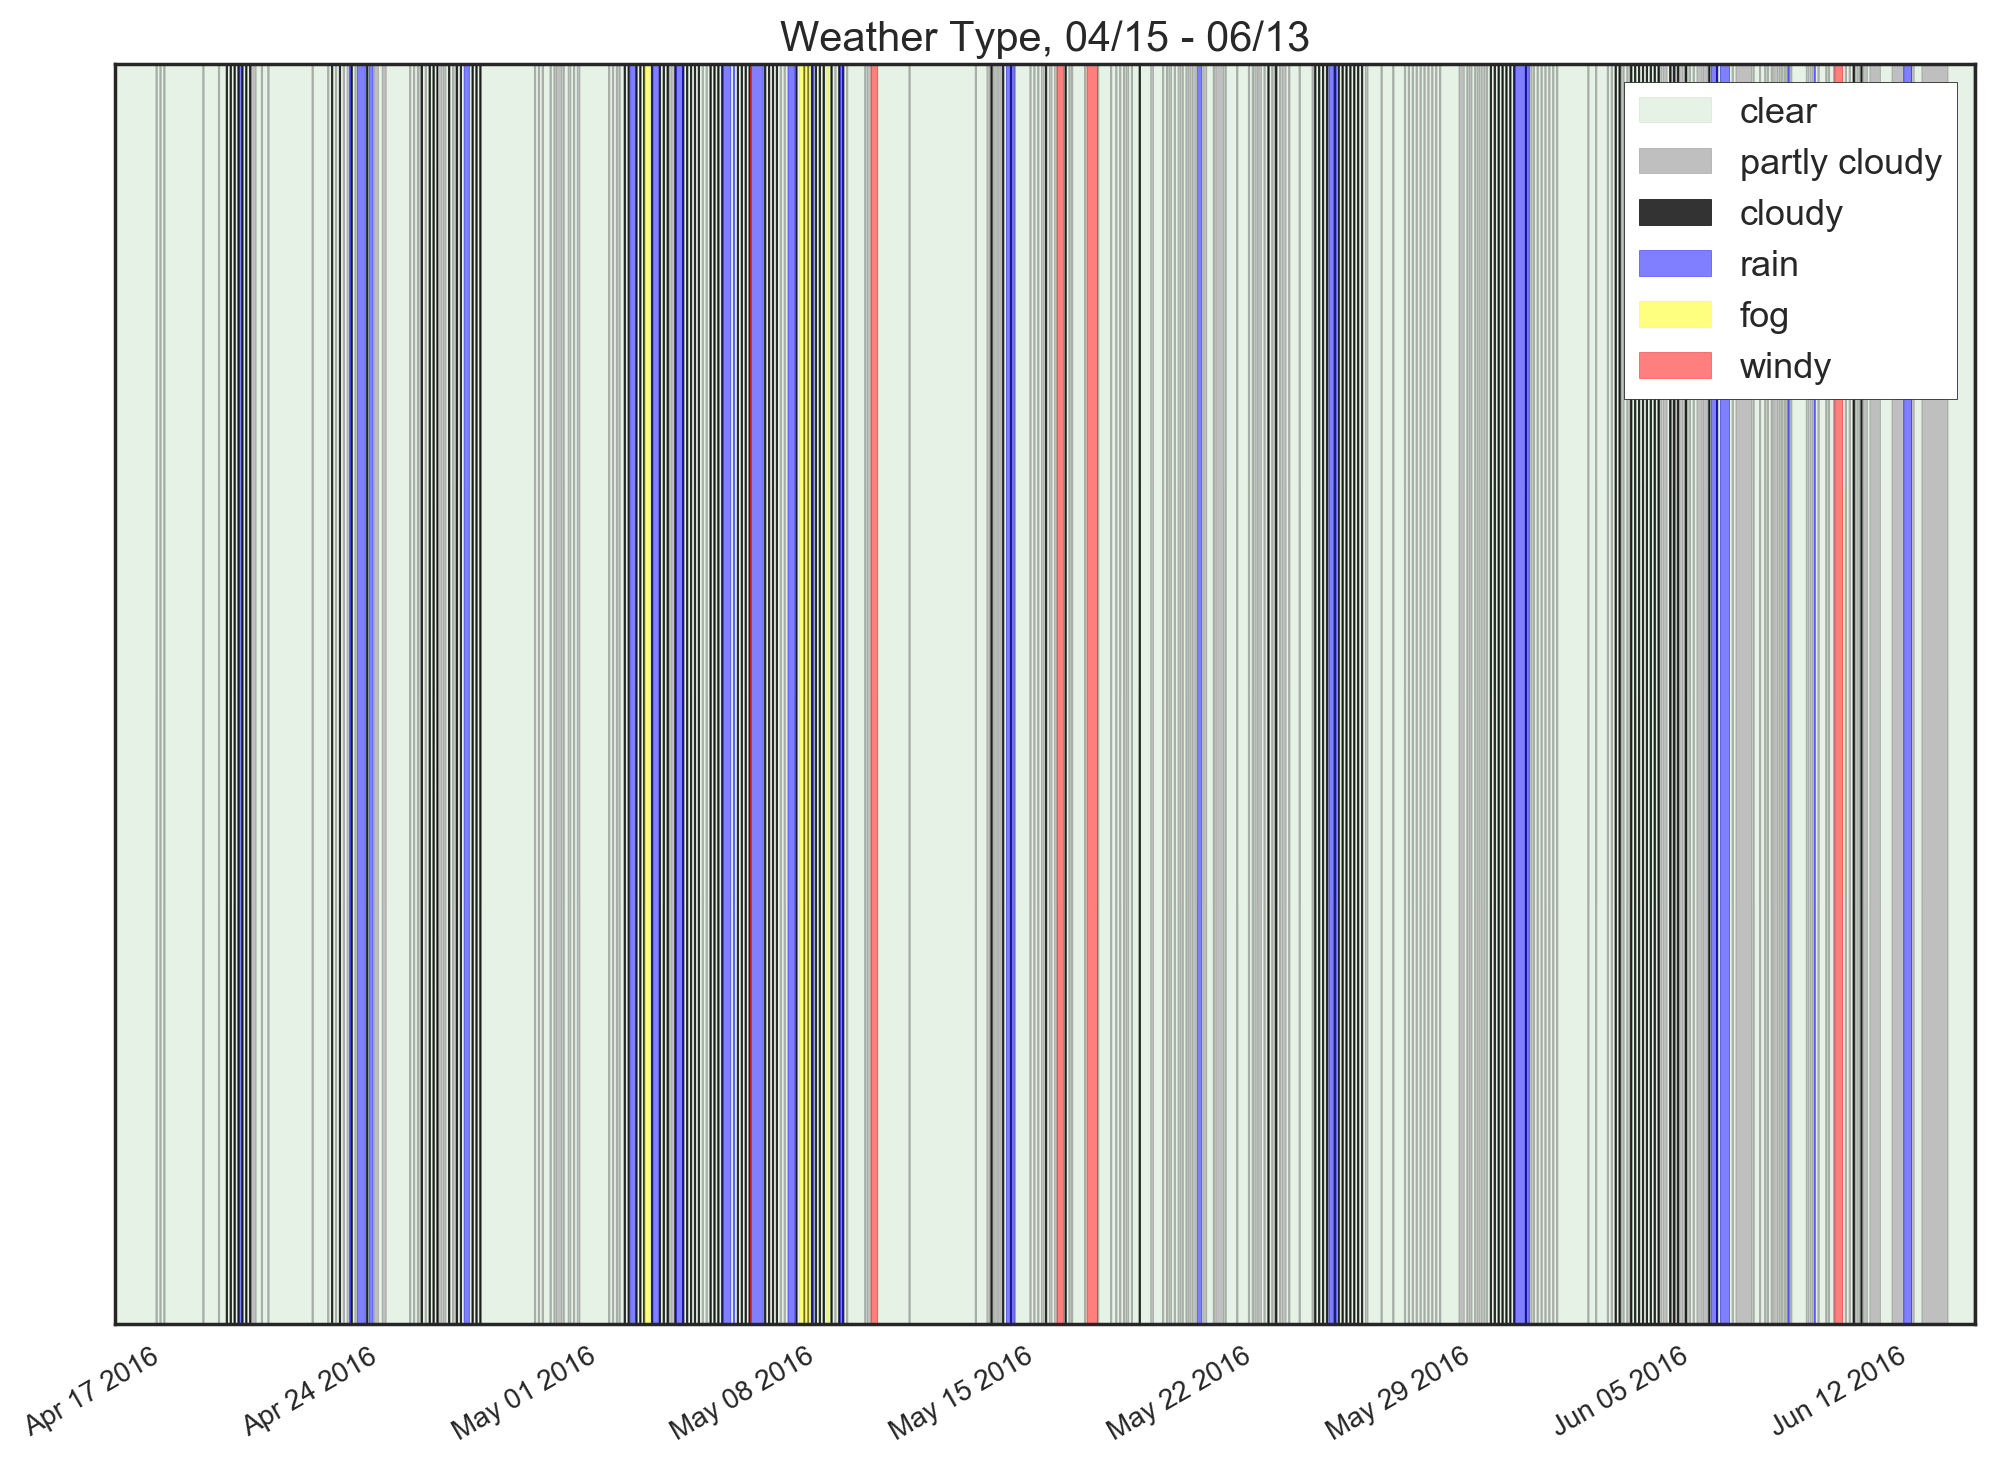
\includegraphics[width=\textwidth-0.5cm]{figs/weather}               
 	 \caption{Weather during Test Period}
  	\label{fig:weather}
\end{figure}


From April 15th through May 23rd (38 days with one 40 minute service break), an older set of AlphaSense O3 and CO electrochemical gas sensors were characterized.  This set was calibrated in Dec 2013 (2 years, 4 months old calibration at the start of the test).  55,589 samples of minute-resolution data was collected to characterize these sensors.

From May 23rd to June 13th (21 days), a brand new set of AlphaSense O3+NO2, NO2, and CO electrochemical gas sensors were characterized (5 month old calibration at the start of the test).  30,150 samples were collected to characterize these sensors.

The two tests of an older and newer set of the same type of Alphasense sensors (O3 and CO) can provide interesting insights-- by comparing the data between the two tests we may be able to draw insights into age- and use-related differences.  By combining the two sets after calibration, we have a long set of data spanning several months to test predictive techniques with.  Assuming the underlying failure modes are the same for sensors of the same make/model, this combined set should be useful at providing insight into the underlying device mechanics.

From April 15th through June 6th (52 days, with two 40 minute service outages), a new SmartCitizen sensor-- with its NO2 and CO sensors-- was installed and running at the MassDEP site.  This sensor gave 85,739 minute-resolved samples.

Finally, from April 15th through June 13th (59 days), our Sharp Particulate Sensor collected samples that we resolved to 1 hour intervals, to match the MassDEP BAM reference.  1,431 samples were collected from this technique.  

\FloatBarrier
\begin{figure}[htb]
 	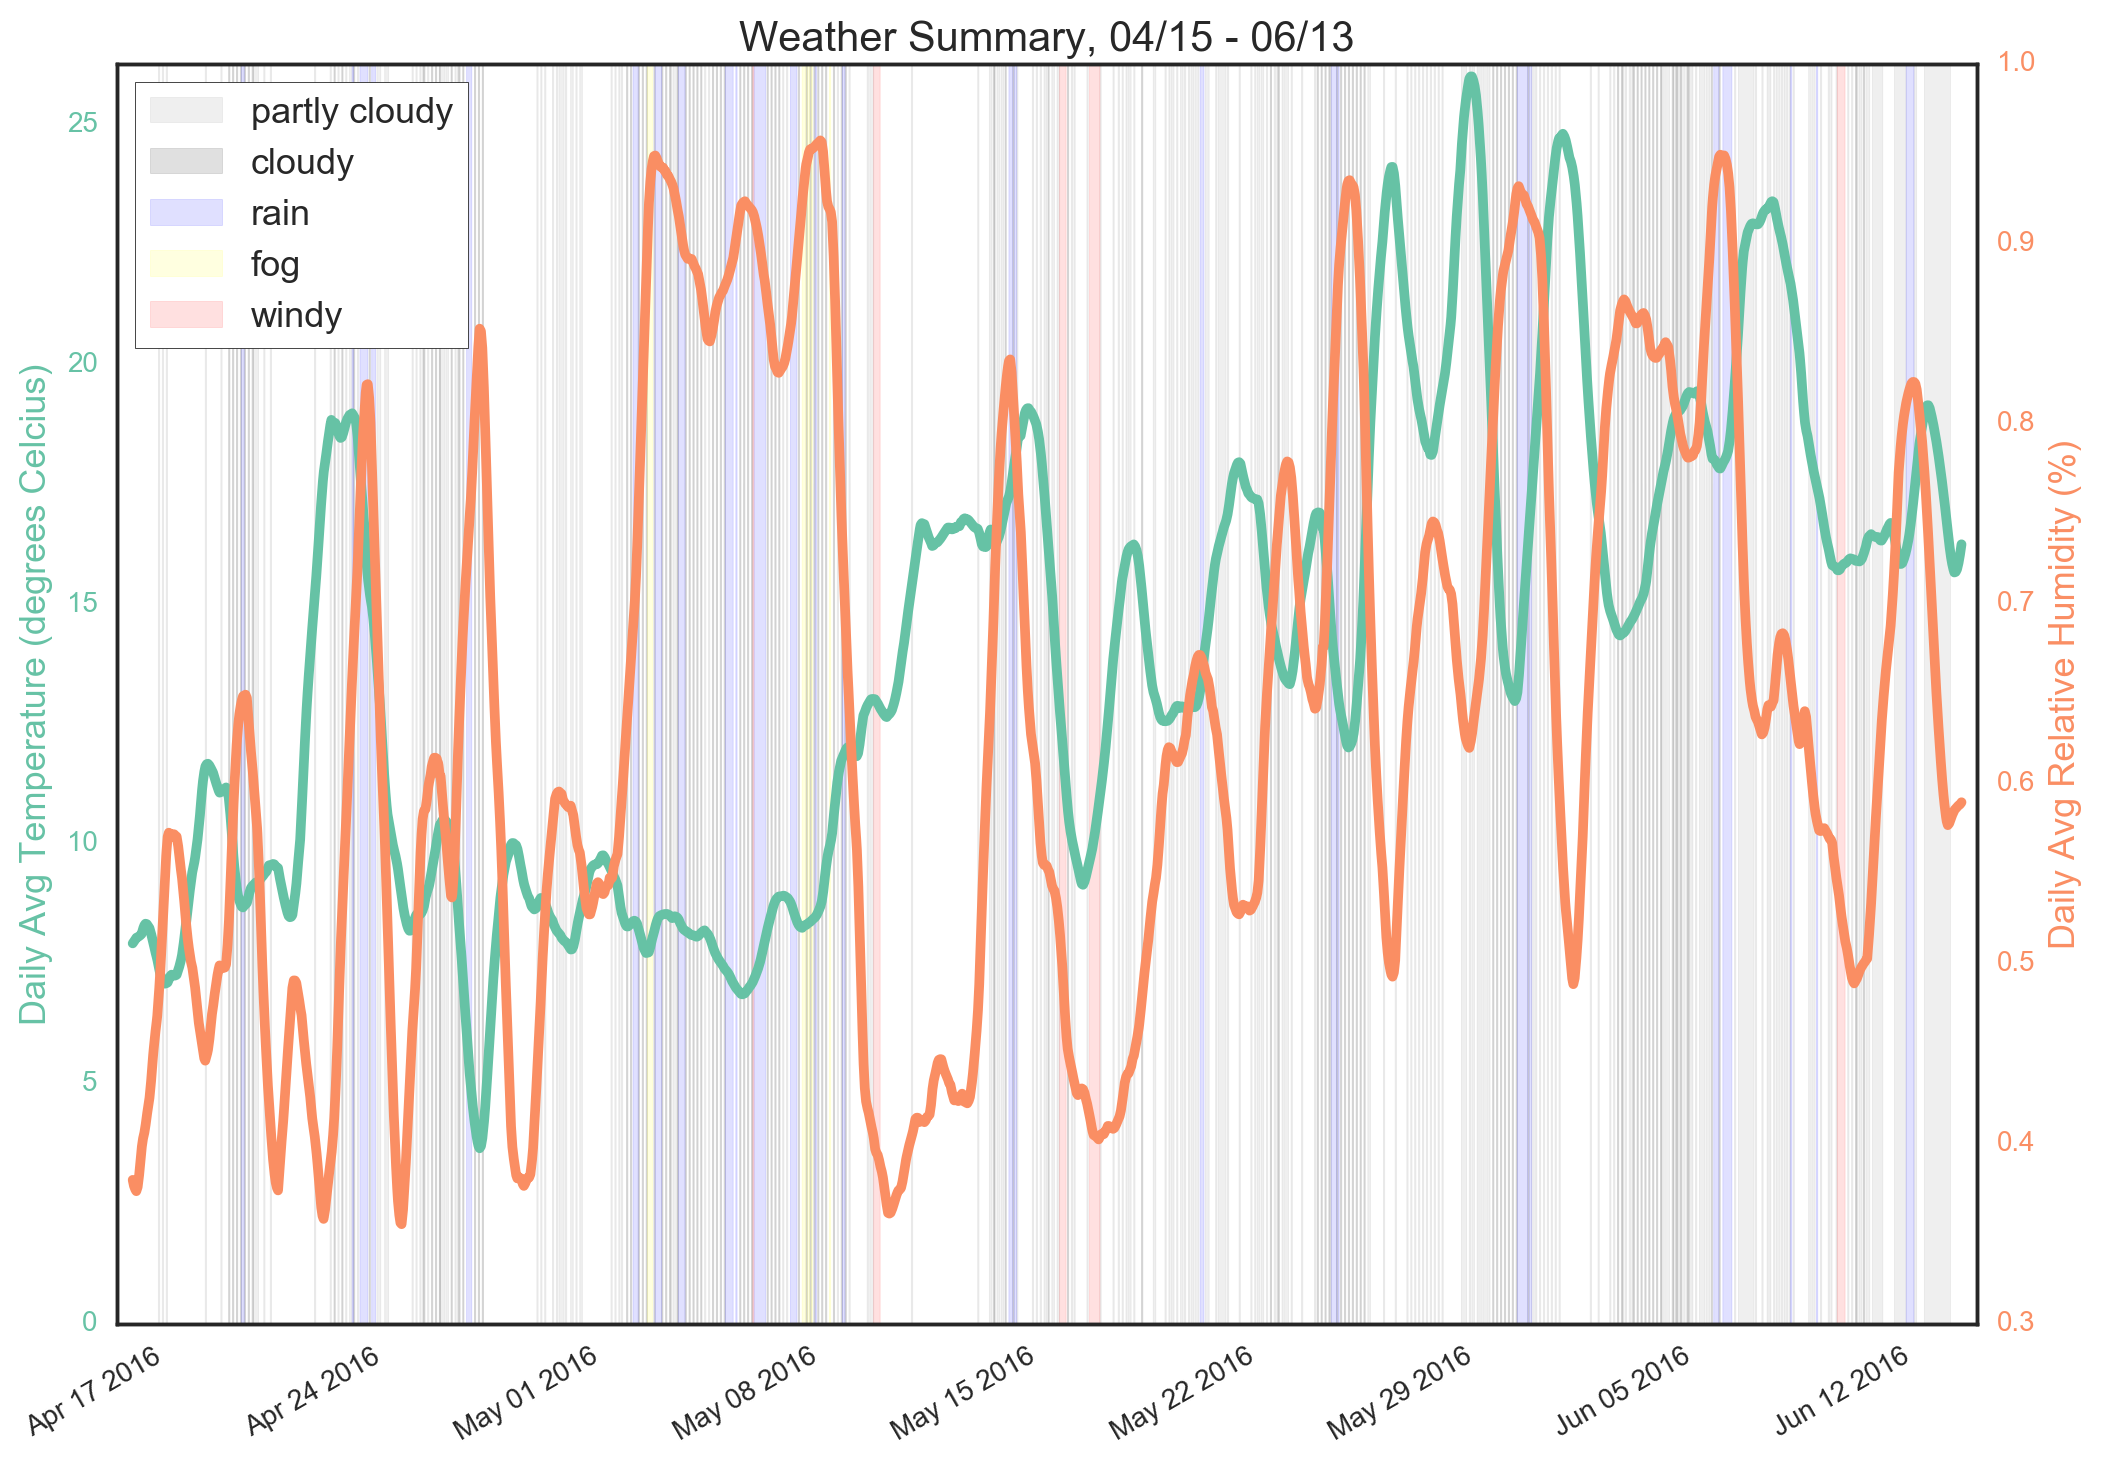
\includegraphics[width=\textwidth]{figs/weather_summary}               
 	\caption{Temperature and Humidity during Test Period}
  	\label{fig:weather_summary}
\end{figure}
\FloatBarrier

The co-location tests started with snow on the ground and ended with summer heat.  External temperatures varied from below 5 to above 30 degrees Celcius, and the relative humidity ranged from 20-100\%.  The weather during the period was nicely varied, with a few foggy days, a few windy days, and a particularly rainy week in early May.  See Figures \ref{fig:weather} and \ref{fig:weather_summary} for details, and Appendix D for more information about trends in ambient pressure, dew, light level, precipitation amount, and cloud cover over the course of the testing period.   
\FloatBarrier

\section{Overview of Data Pre-Processing and ML Strategy}
All readings taken by the co-located sensor were measured in 30 second intervals, and timestamped using the on-board Real Time Clock before being saved to an SD card.  Since this was all done offline, no corrections for the timestamps could be applied.

In general, we found a 0.15-0.25\% drift in the RTC timestamps.  This results in 60-200 samples of error every three weeks or so.  To appropriately align these drifted, ~30 second values with our minute-resolved reference values, we applied two stages of correction.  To begin, we corrected the timestamps to reflect their actual time (assuming a constant delay between each, and knowing the precise time the measurements started and ended).  We then linearly interpolated between these corrected timestamp values to find on-the-minute values for every minute.

For the hour long samples of BAM data, we had to consolidate our minute data down to hourly values.  To match the process of the BAM sensor (which collects samples for the first 50 minutes of every hour, and measures for the last ten), we wrote a script to average every value in our machine learning arrays over the course of the first 50 minute of every hour, and throw away the last 10.

This is only the first step of pre-processing the data, however.  For our air quality signals, a calibration step is necessary before comparing the data and characterizing the sensor.  For the SmartCitizen CO and NO2 sensors, as well as for the Sharp particle sensor, their output is an uncalibrated mV value.  In the case of the Sharp sensor, the reading is inverted from the actual particle level (as it is a measure of light that makes it through the sensor without scattering).  These sensors were calibrated using a LMSE approach to optimize a simple scale factor or a scale factor and an offset.  The minimization function was run (1) on all of the data, (2) with the outliers (> 1 stdev) removed, (3) on long-term averages of the data, and (3) to only optimize values that were within some tolerance (throwing out sections that appeared to show disagreement and instead favoring a tighter fit on aligned data).  The most realistic, quality fit was chosen from amongst these options as the `calibrated' reference.

For the AlphaSense sensors, calibration was even more complicated.  These sensors come with a calibration sheet giving appropriate values.  The formula for most of their sensors is: {\small \[ppb = \frac{(we - we_{zero}) - (n*ae - ae_{zero})}{sensitivity}\]} where $we$ is the working electrode measurement in mV, $ae$ is the auxiliary electrode measurement in mV, $we_{zero}$ is the working electrode offset value in mV, $ae_{zero}$ is the auxiliary electrode offset value in mV, $n$ is a temperature dependent and sensor chemistry dependent scale factor, and the sensitivity is the mV/ppb gain factor of the instrumentation amplifier on the conditioning board.  For the cross-sensitive O3+NO2 reading, we use the calibrated NO2 values and subtract the resulting mV offset given the calibrated NO2 sensitivty: {\small \[ppb = \frac{(we - we_{zero}) - (n*ae - ae_{zero}) - \frac{no2_{ppb}}{x\_sensitivity\_to\_no2}}{sensitivity}\]} While we tried the provided calibration data-- as well as simple LMSE scaling-- we found the best agreement came from LMSE minimization using a bounded search of $we_{zero},  ae_{zero},$ and $sensitivity$.  In these cases, the seed values were the provided calibration terms from AlphaSense.  This type of calibration gave very strong results compared to other methods.

With calibrated data, an appropriate tolerance was chosen for each sensor value (typically $\pm$2-5\% of the full range, though a larger tolerance was chosen for particulate), and each reading was classified as `correct' if falling within that tolerance of the MassDEP reference measurement, or `incorrect' if falling outside of it. 

This data is now ready for machine learning using the logistic regression discussed in the introduction to this chapter.  We performed all of this analysis using python's scikit-learn machine learning toolbox-- however, some experimentation was done with the java-based (GUI driven) `Weka' toolkit (using a python ARFF file conversion library), as well as initial exploration with google's new tensor-flow library (which has logistic regression support, but which really shines for its deep learning ability and large dataset handling).  These additions tools, and additional techniques, will be explored in more depth in the near future.

The general outline of the machine learning process we applied to the data is as follows: (1) load in the feature values (approximately 150 of them) to predict our binary error classification, (2) impute (or fill in) missing values, (3) split our data into training and test sets used 5-fold cross-validation, (4) run a grid search over logistic regression parameter-space to find the best regularization coefficient and penalty terms, (5) train our new 'best model' using the five training sets, and (6) verify the results on the five test sets.  Importantly, two types of cross-validation are used-- a shuffled type and a chunked type.  In one case, data from the entire two month period is randomly selected to constitute training and test sets; in the other, the first several weeks are used to predict the last, the last several are used to predict the first, etc.  The difference in these results gives us important insight into algorithm robustness and the effect of seasonal variation on our predictions.  

Additionally, we use randomized decision trees to rank the importance of our features, as well as seven other feature reduction techniques (correlation, linear regression, random forest, lasso, RFE, ridge, and stability).  A reduced set of the top 15 features is then used to retrain our original Logistic Regression, and the results are compared.  The strength of agreement between feature reduction techniques can suggest meaningful predictive relationships, and the relative strength of the classifier with this reduced feature set can also corroborate strong causality for the top features.

There are two main metrics we use to evaluate our system performance.  The most obvious metric is to compare the right answer ('is the sensor actually in error?') with the predicted one ('do we think the sensor is in error?') and display our results in a 2x2 confusion matrix.  We can easily calculate the error rate of our algorithm from this matrix.

Logistic Regression offers a probability along with its prediction, however, so to fully evaluate the strength of our results we must take these probabilities into account.  Our second evaluation metric-- and the accepted standard for this type of evaluation-- is a Receiver Operating Characteristic (ROC) curve.  This curve plots the true positive rate (the number of correct predictions that a measurement is in error, normalized by the total number of errored air quality readings) against the false positive rate (the number of incorrect predictions that a measurement is in error normalized by the total number of accurate air quality readings).  We can compute a point on this graph by choosing an arbitrary threshold for our probability, and classifying every measurement as a predicting an error in our reading or not based on whether the probability that it is falls above or below this threshold value.  If we set our probability threshold at 50\%, we find the point corresponding to our original confusion matrix.

When we plot the points for every threshold value (from 0-100\%), we generate an ROC curve.  These curves start at (0,0) and end at (1,1) on our plot.  Random guessing will form a line between the points at a 45 degree angle.  Perfect accuracy with 100\% confidence will form a right triangle-- jumping immediately to a value of (0,1) on our graph before continuing horizontally over and meeting up with the upper right corner.  Real, meaningful predictions will likely fall somewhere in between.  The area under the ROC curve (AUC-ROC) is normalized to a value between 0 and 1, and frequently used to characterize the quality of predictions generated by our logistic regression in a more comprehensive way than a simple confusion matrix.  Generally speaking, values above 0.8 suggest our model has good-to-excellent predictive power as the number grows closer to one, and values above 0.7 represent reasonable predictions.  Values below this mark are marginal, with anything close to 0.5 suggesting total failure.

Once we've found the AUC-ROC for our optimized logistic regression, we compare the results for the 5-fold validation sets (one having been `shuffled' or randomized, and the other having been `chunked').  The shuffled version assumes no time dependent phenomena-- using randomly chosen samples throughout the entire test to predict random other samples interspersed throughout the test.  The chunked version is a more realistic model-- using data we've already gathered from one period of time to predict future data.  

We must be careful with the shuffled version-- errors frequently occur together in time (a sensor will misread for an hour or two in a row, giving a few hundred errors at once, likely because of underlying phenomena).  Monotonically increasing functions (like temperature) could serve as a proxy for time, and the algorithm might take advantage of this co-occurance to `predict' our error.  This is a classic example of overfit, and it should be simply to look at the underlying feature and error distributions to ensure that our model hasn't led us to incorrect conclusions.  This could lead to artificially strong results in the shuffled case.  If we see a strong predictive relationship for one of these variables in the shuffled case, it is important to make sure that the variable is not simply monotonic and co-occuring with one large window of consecutive poor readings.  

After verifying the quality of our shuffled results, we can compare the shuffled and blocked versions of the algorithm.  If the shuffled version still does substantially better than the block-wise version, it suggests that we haven't trained on enough data to capture season-agnostic predictive information.  However, when the two agree, it forms a powerful indication that (1) we've captured enough data to train across seasons, and (2) we have hit upon real and useful phenomena.  
\FloatBarrier

\section{Machine Learning Features}
In most of these applications, around 150 features were used to train our machine learning algorithms.  Features were either measured from the learnAir system or harvested from the Forecast.IO weather API.  A few additional features (the EPA reference black carbon, wind speed, and wind direction measurements) were all included as training features.  Raw sensor signals are included as well as their calibrated versions.  Many of these signals were further manipulated or processed to give more derived features.  

The measured set of features represents data collected from on-board sensors-- temperature, humidity, noise, light, vibration, pressure/airflow, and other air pollution sensors.  We also include the signal from the sensor whose quality we're trying to predict as well (if it reads in certain ranges or slews at a certain rate, we may be able to assume that the sensor is out of its useful range).  

\begin{marginfigure}
 	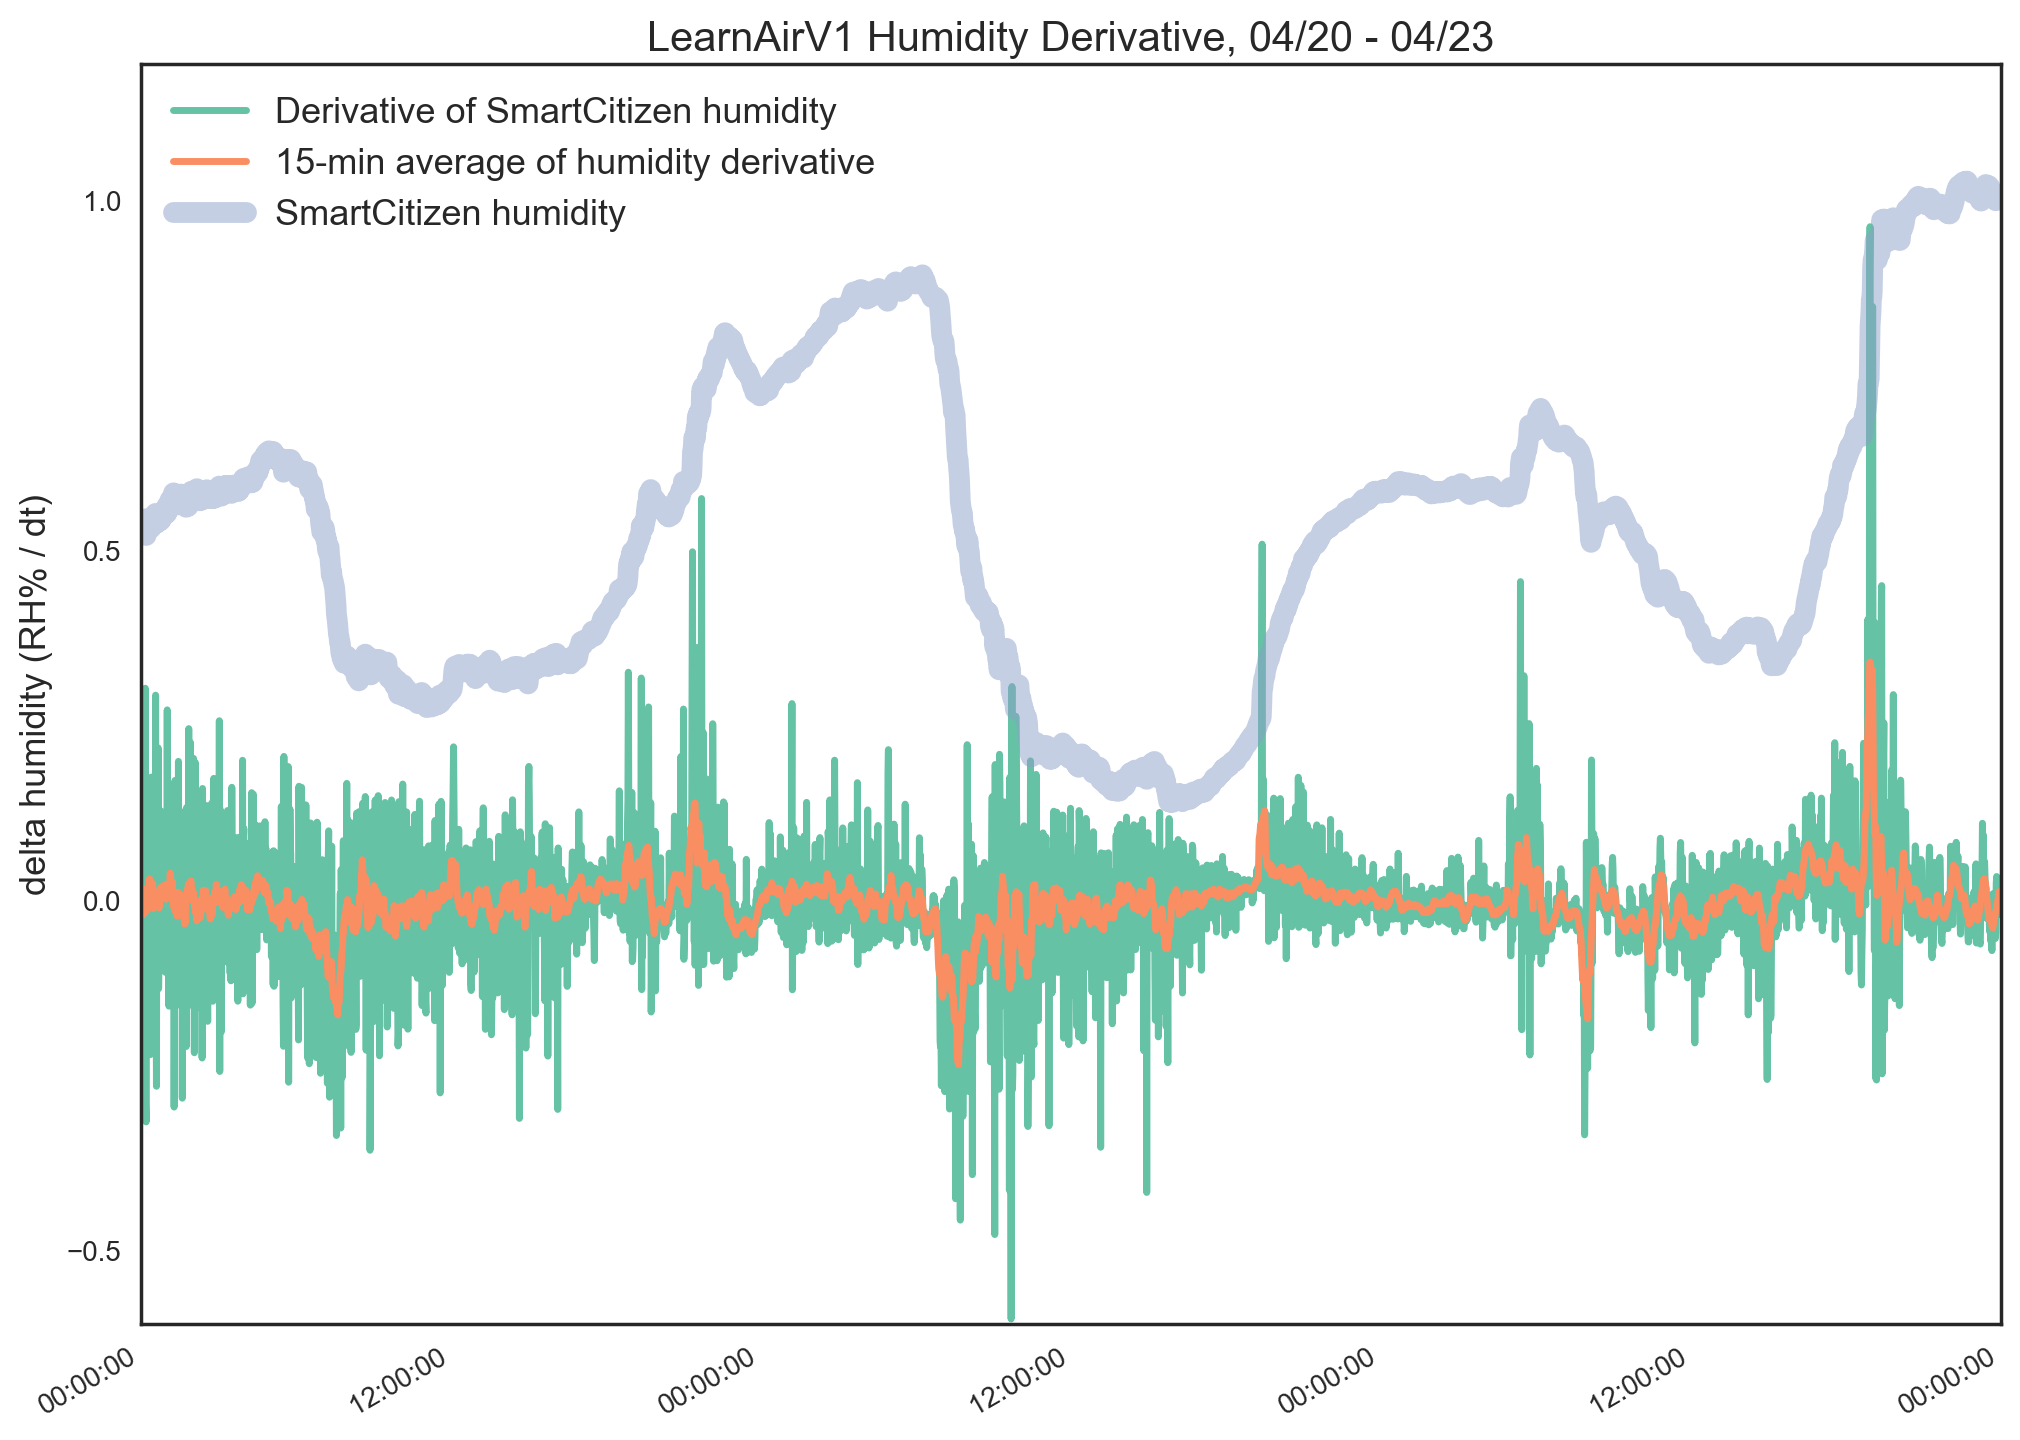
\includegraphics[width=\textwidth]{figs/humidity_derivative}               
 	 \caption{Humidity Derivative Feature Creation}
  	\label{fig:humidity_derivative}
\end{marginfigure}

For most of the main features, we created derivative features to predict errors resulting from rapid changes in environmental conditions (anecdotally, we know this to be true for electrochemical sensors).  We also looked at intelligently chosen averages over time-- ones that minimized quantization errors, smoothed data to match the EPA reference, or whose averaging gave evidence of longer term trends that might also be important in analyzing sensor state and measurement quality.


\begin{figure}[htb]
\centering
 	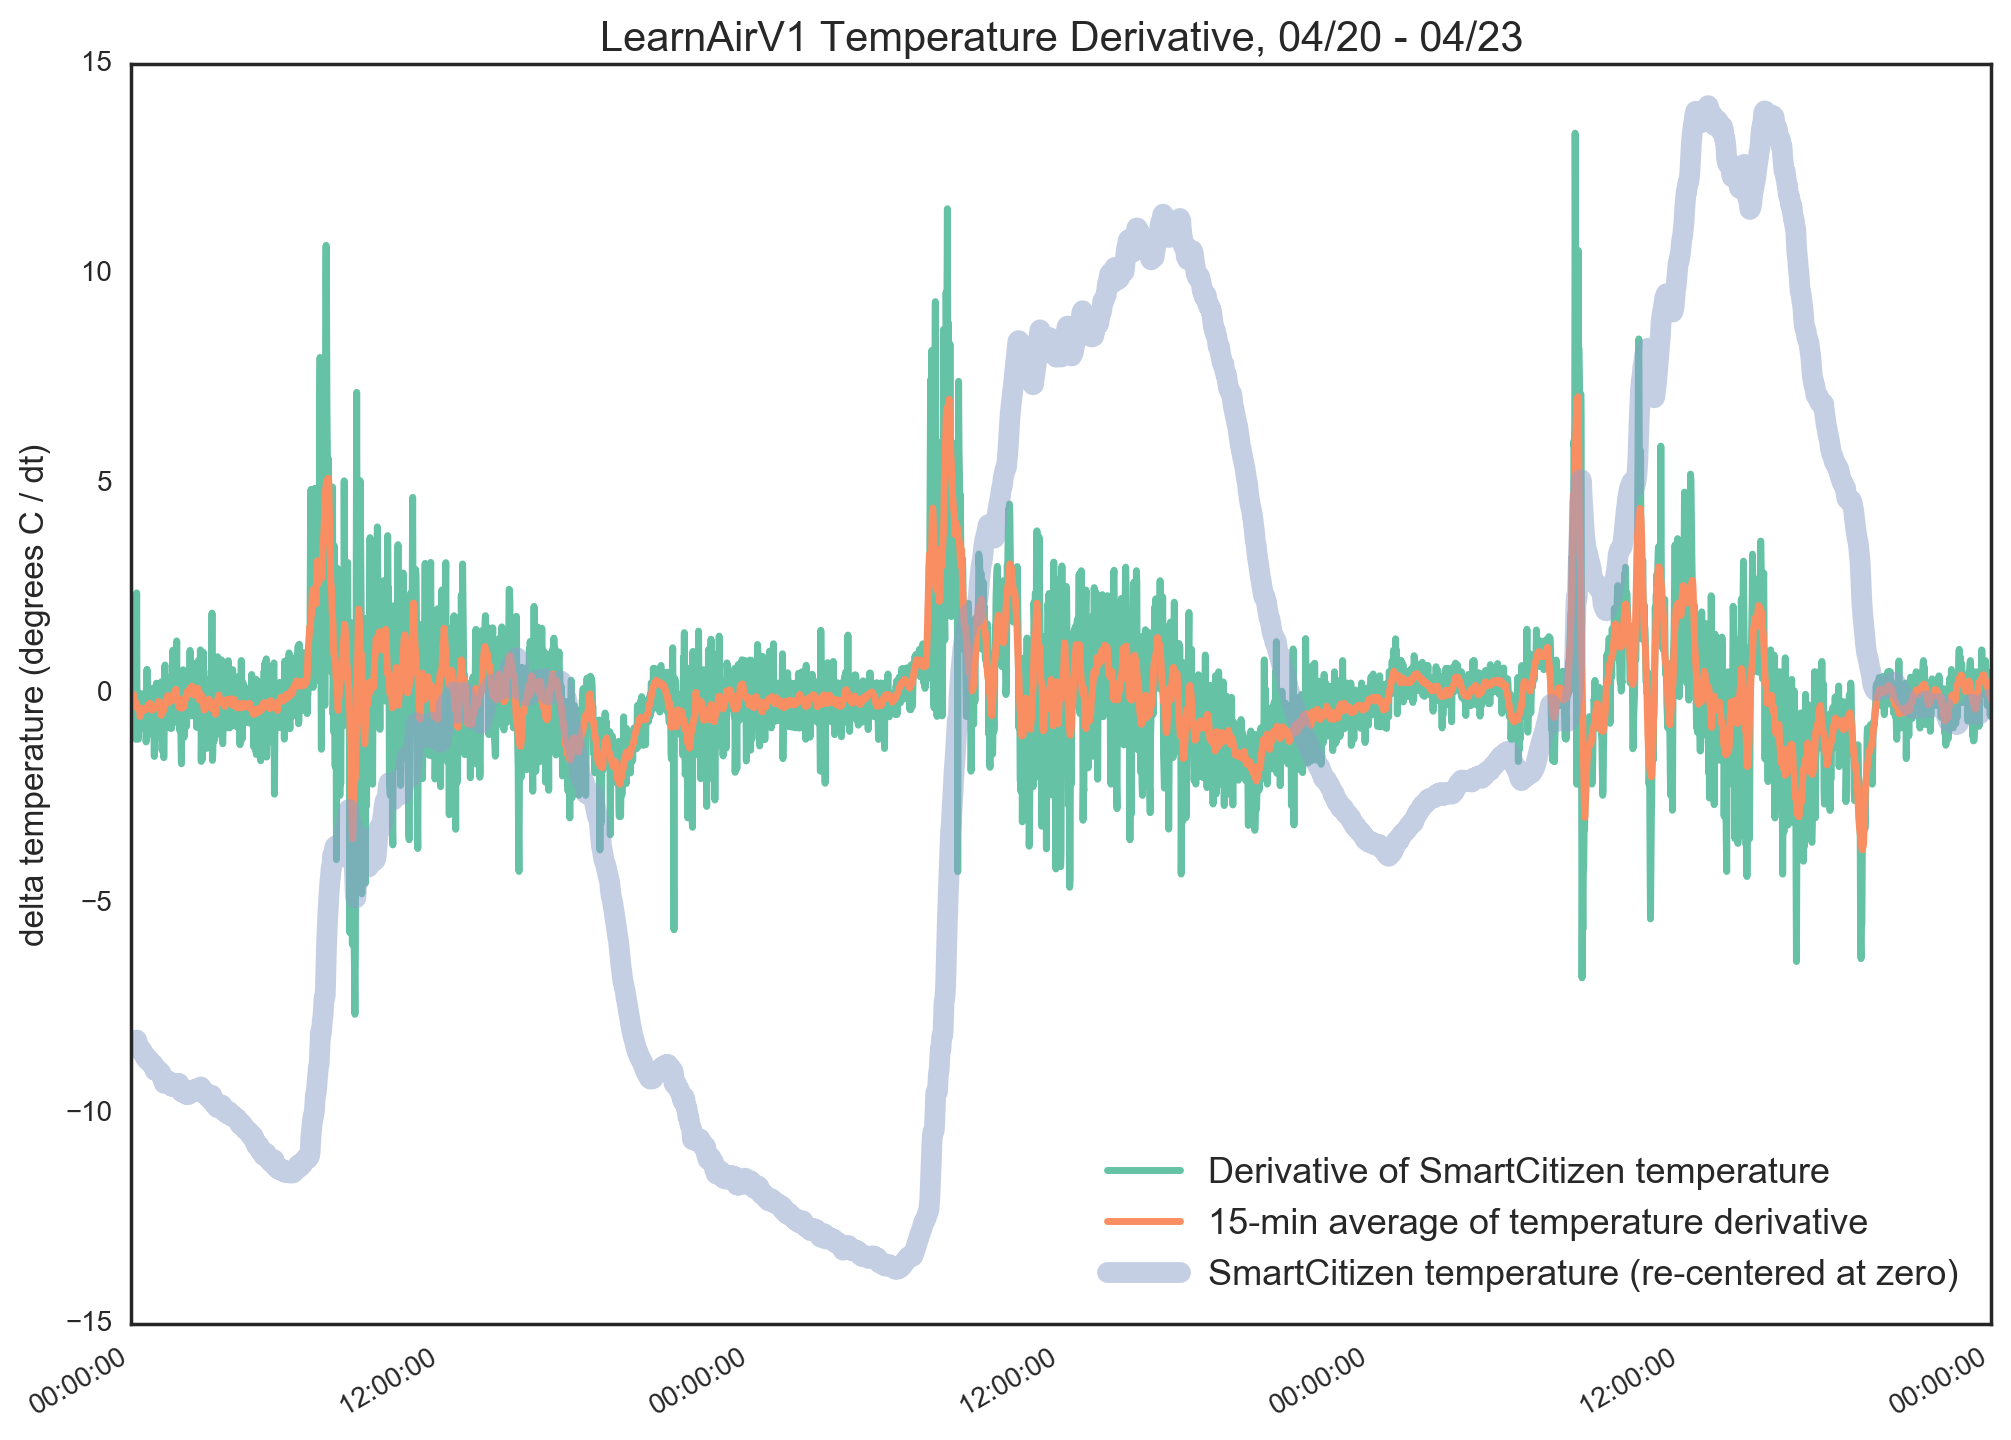
\includegraphics[width=\textwidth-2cm]{figs/temp_derivative}               
 	 \caption{Temperature Derivative Feature Creation}
  	\label{fig:temp_derivative}
\end{figure}



Several API's were evaluated for use in this project, and Forecast.IO stood out as a well-reputed option.  They use machine learning to combine many weather forecast APIs into one highly accurate dataset.  The Forecast.IO data comes in hourly intervals, so a running 60 minute average was used to interpolate the values to minute resolution (most of the measured fields, like temperature, are relatively slow-moving).  For class-based indicators (for instance, the `weather-summary' field indicating `cloudy', `windy', `foggy', `rainy', etc) we converted the API value into binary fields that matched each class.   

We created features such as `temperature differential' and `humidity differential' -- a constructed feature that corresponds to the difference in measurement between the ambient conditions (as measured by Forecast.IO) and the conditions in the box (as measured by the SmartCitizen Kit).  While these features are linear combinations of other features (and thus won't improve our model's predictive power), they serve an intuitive purpose, and may help reduce the feature set (mapping two features to one) if they turn out to be important indicators of performance.
 
\begin{figure}[htb]
\centering
 	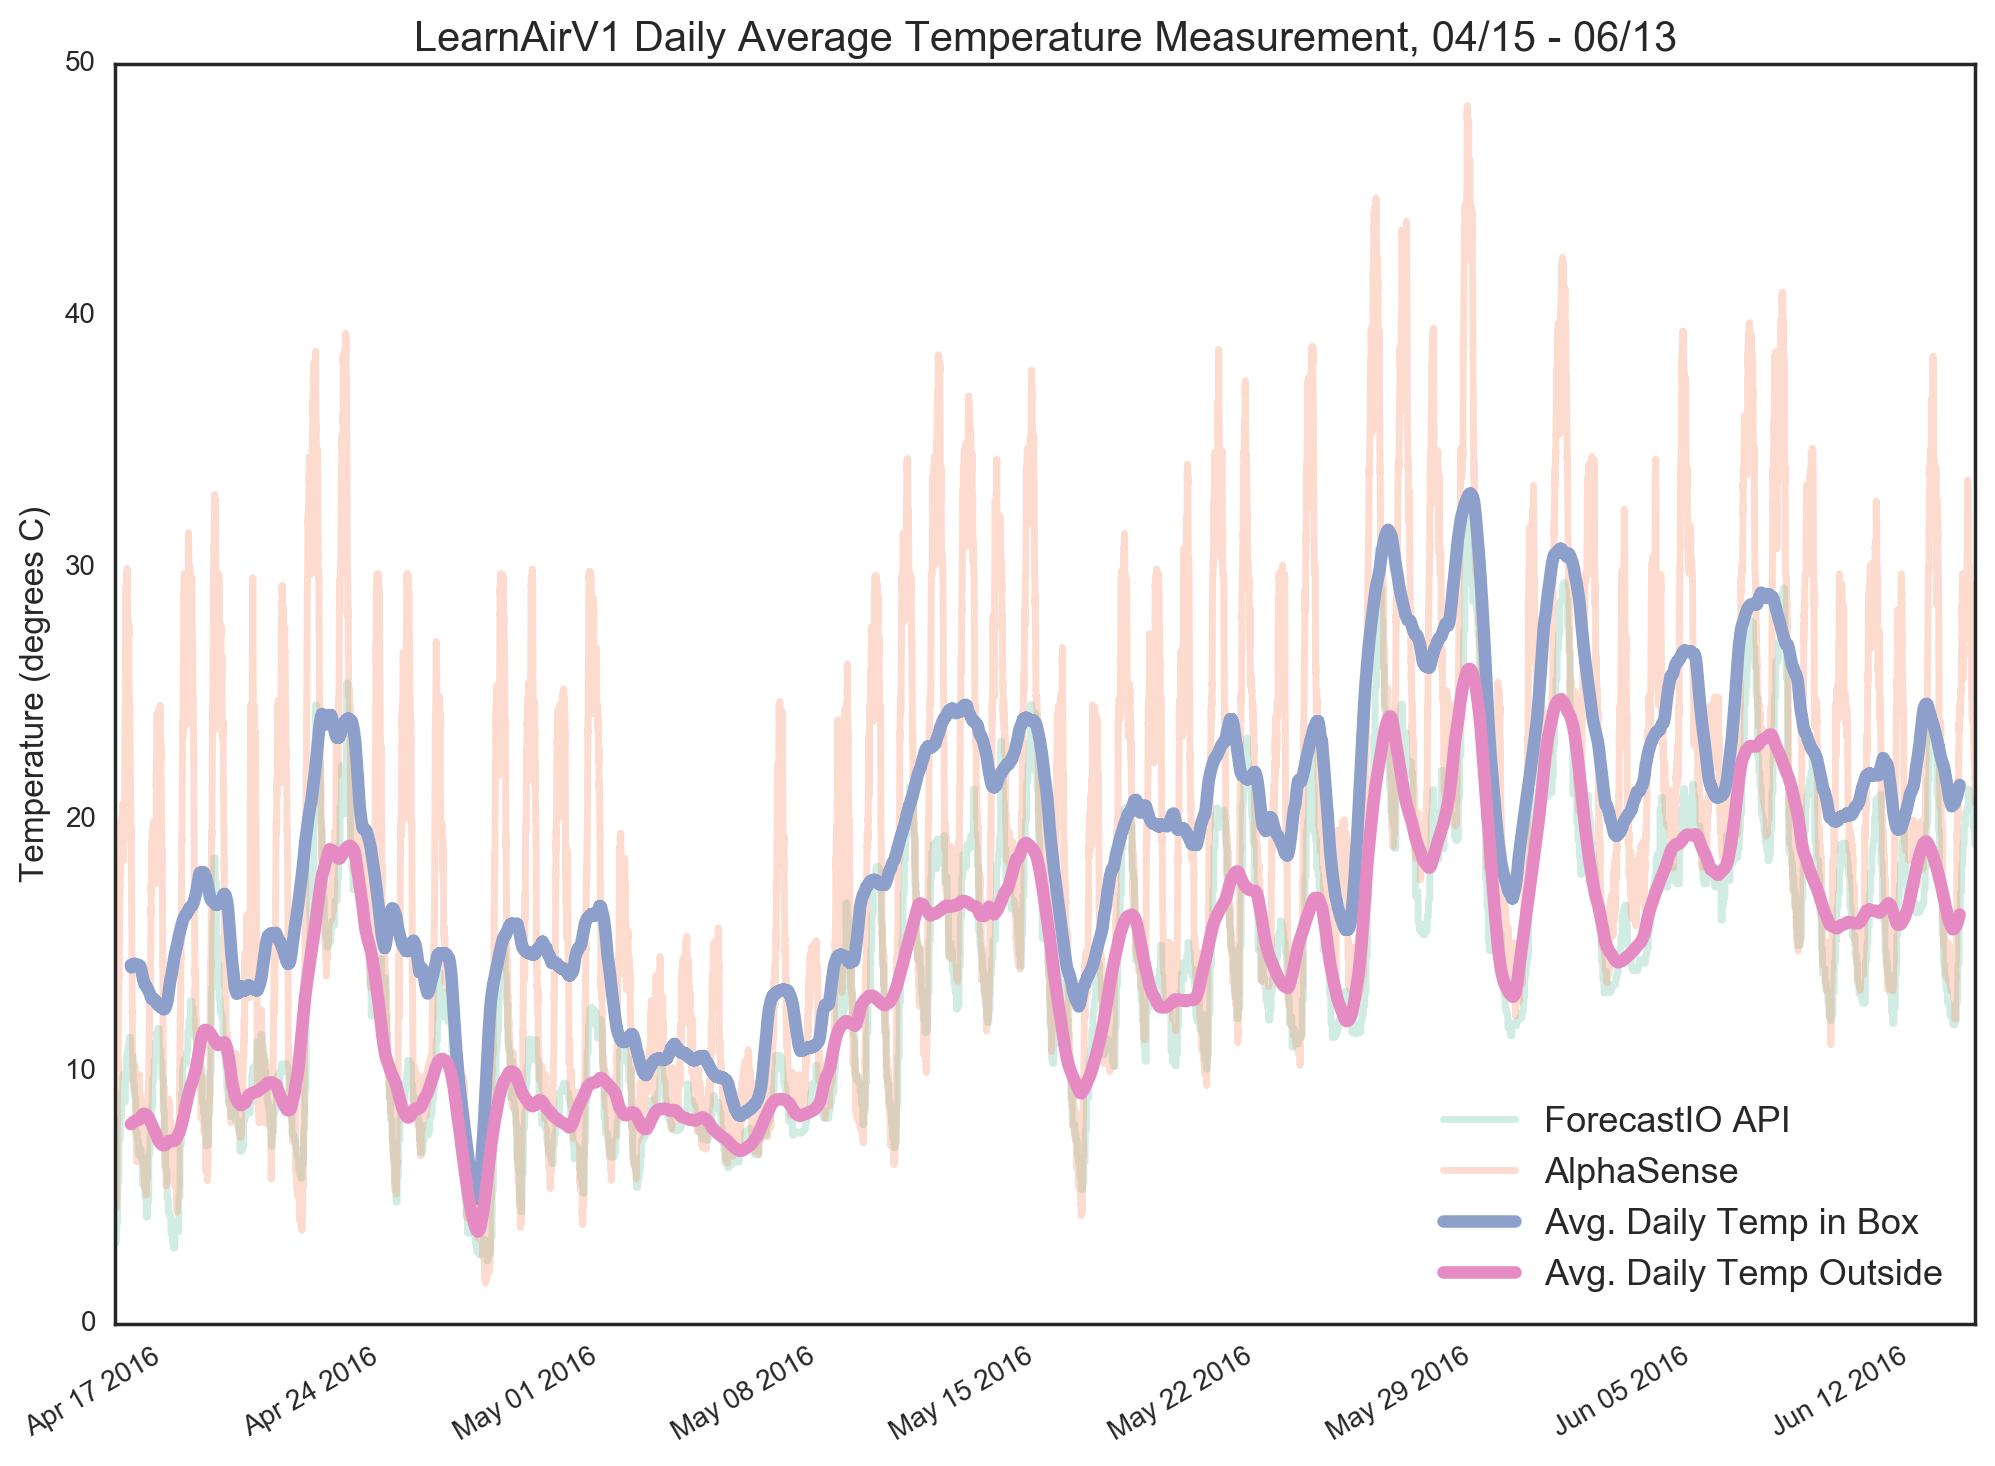
\includegraphics[width=\textwidth-2cm]{figs/temp_daily}               
 	 \caption{Temperature Inside vs. Outside the Device during Test Period}
  	\label{fig:temp_daily}
\end{figure}

\begin{figure}[htb]
\centering
 	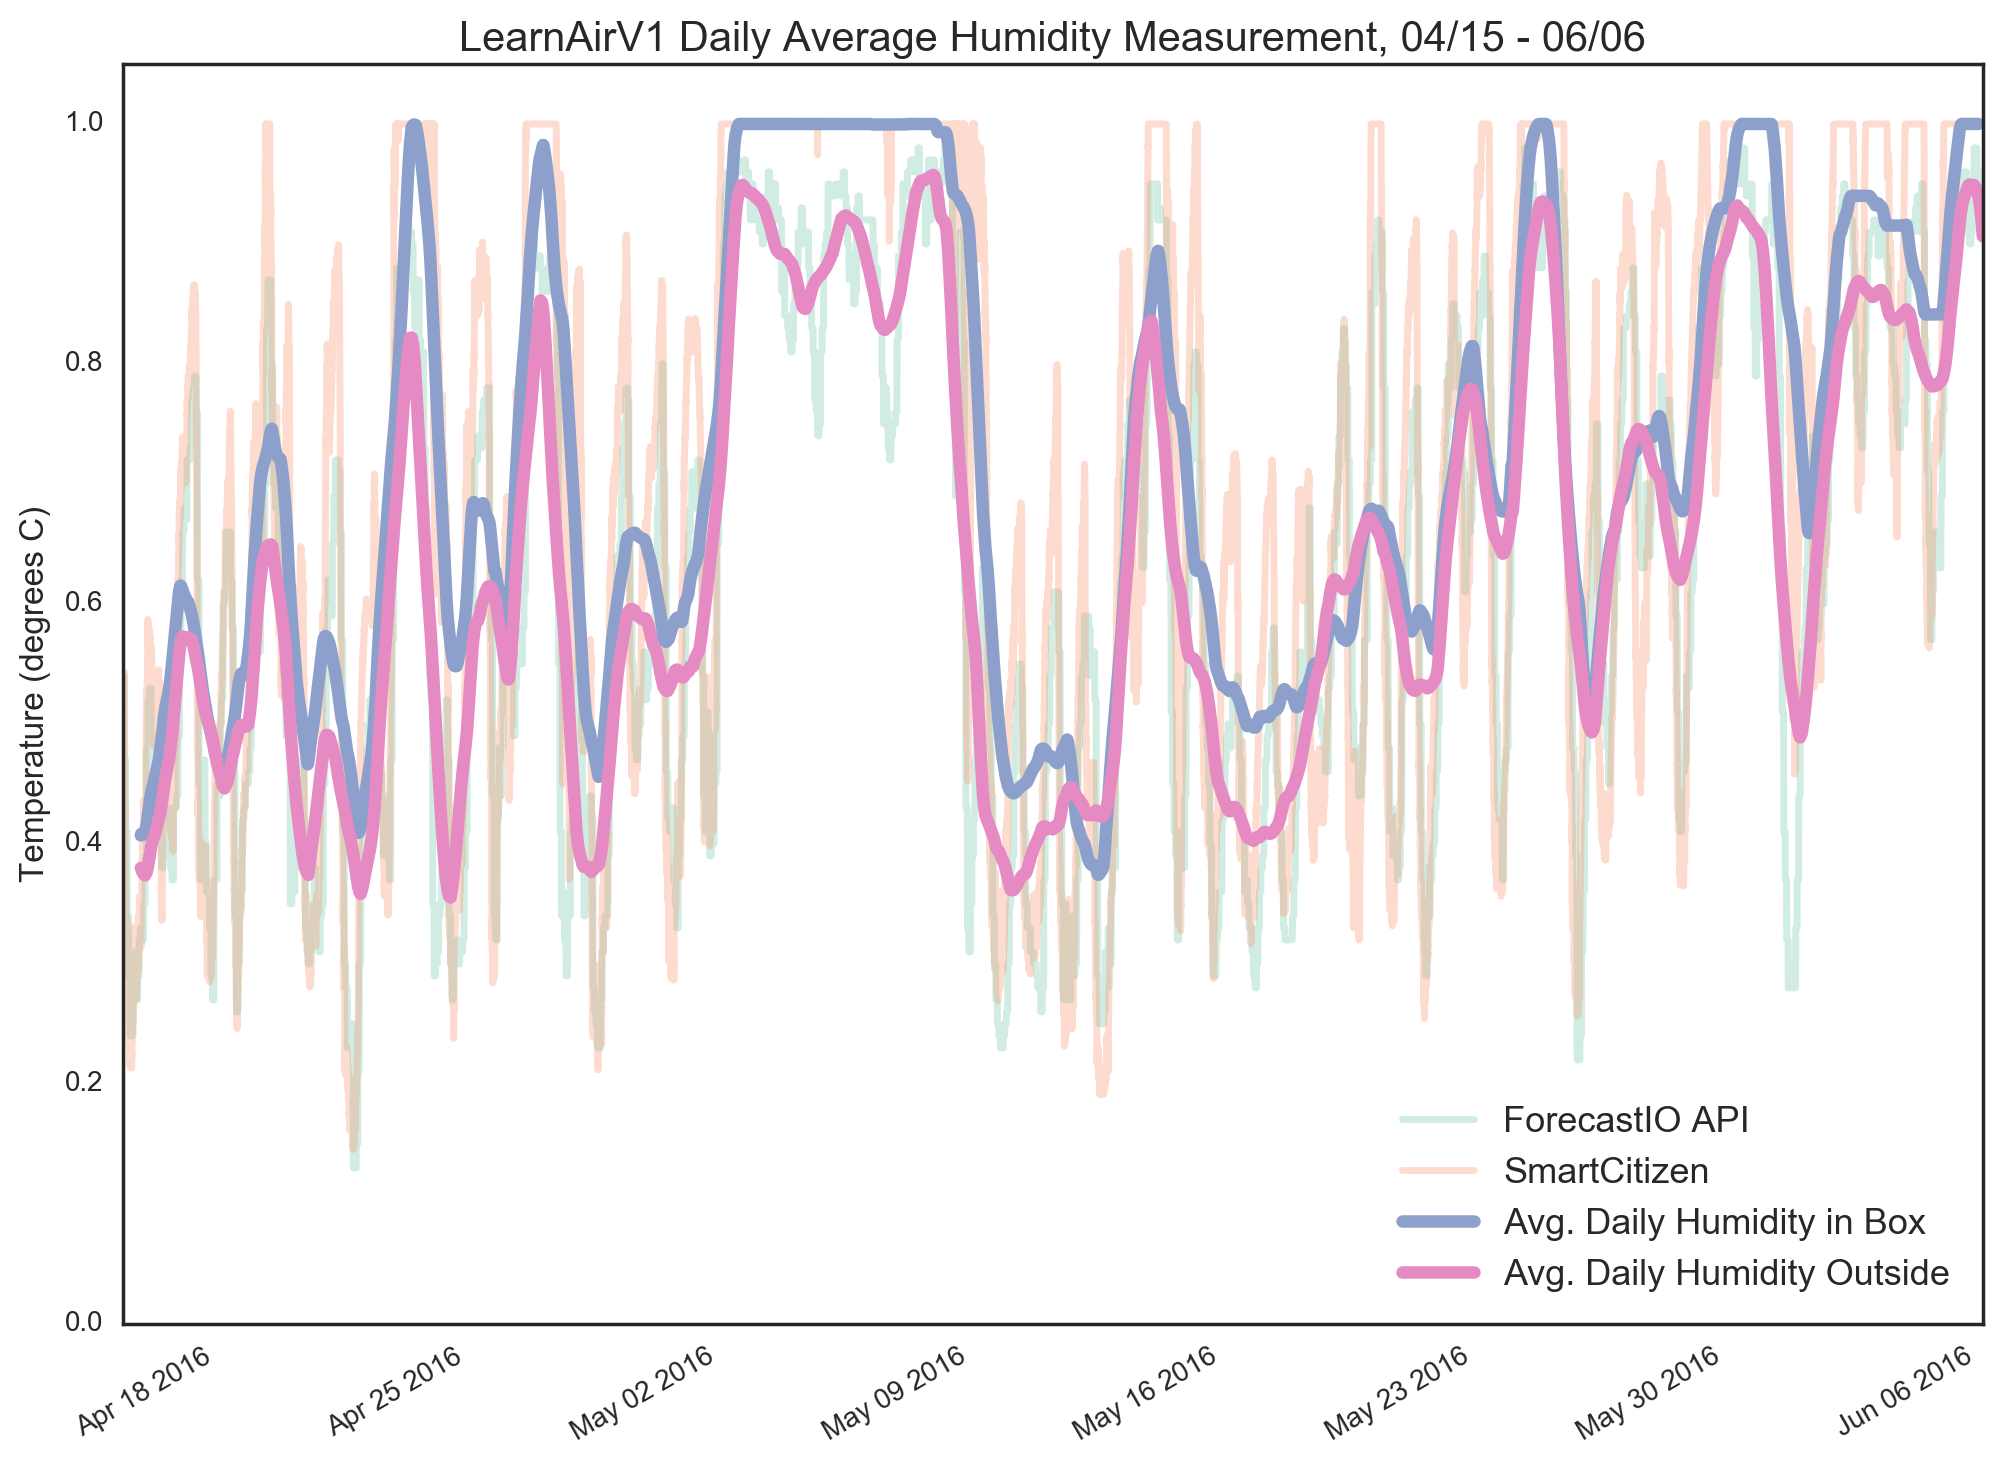
\includegraphics[width=\textwidth - 2cm]{figs/humidity_daily}               
 	 \caption{Humidity Inside vs. Outside the Device during Test Period}
  	\label{fig:humidity_daily}
\end{figure}

Finally, we added some features to represent other potentially important quantities.  These features include the time of day (including features for morning and evening rush hours), the day of the year (mapping to the season), and the elapsed time since the device was plugged in (for `warming up' effects).

In general, some small subset of features was removed for each training session.  For instance, the higher quality Alphasense CO sensor was removed as a feature when training the less capable SmartCitizen CO sensor.  (Training with this feature gives incredibly high accuracy at predicting failure, because it is effectively training itself with the answer.)  By training with comparable or cheaper sensors, we can assess the likelihood of a cheap system working predictably.

In most cases, the EPA reference black carbon sensor data was left as a feature-- while this is not a feasible measurement for a portable, cheap device, it is still useful to know if black carbon is a strong predictor of a sensor's failure.  This knowledge allows us to infer something about how the sensor is failing, and what type of sensor we might want to pair it with.  With this technique, the machine learning process is not evaluative of a current system's success-- instead, it works as an exploratory tool that might inform a potential system design.

The next page includes a list of the main features.  Processed, calibrated, and other derived features extend this list to the complete set.  For histogram plots of many of the main features (made using Weka), see Appendix D.

\begin{table}[H]
\small
\centering
\begin{tabular}{lclc|c|}
\\
\\
\toprule
Feature & Type & Description \\
\midrule
AlphaSense \#1 Work Electrode & Continuous & raw signal from alphasense sensor \\
AlphaSense \#1 Aux Electrode & Continuous & raw signal from alphasense sensor \\
AlphaSense \#2 Work Electrode & Continuous & raw signal from alphasense sensor \\
AlphaSense \#2 Aux Electrode & Continuous & raw signal from alphasense sensor \\
AlphaSense \#3 Work Electrode & Continuous & raw signal from alphasense sensor \\
AlphaSense \#3 Aux Electrode & Continuous & raw signal from alphasense sensor \\
AlphaSense O3 & Continuous & calibrated signal from raw electrode readings \\
AlphaSense NO2 & Continuous & calibrated signal from raw electrode readings \\
AlphaSense CO & Continuous & calibrated signal from raw electrode readings \\
AlphaSense H2S & Continuous & calibrated signal from raw electrode readings \\
AlphaSense Temperature & Continuous & raw signal from alphasense temp sensor \\
Wind Pressure Reading & Continuous & raw signal from pressure sensor \\
Corrected Wind Reading & Continuous & conditioned pressure signal to relate to wind \\
Sharp Dust Reading & Continuous & raw signal from optical particulate sensor \\
SmartCitizen CO Voltage & Continuous & raw signal from smartCitizen CO sensor \\
SmartCitizen NO2 Voltage & Continuous & raw signal from smartCitizen NO2 sensor \\
SmartCitizen Noise Voltage & Continuous & raw signal from smartCitizen Piezo mic \\
SmartCitizen Humidity Voltage & Continuous & raw signal from smartCitizen SHT15 \\
SmartCitizen Temperature Voltage & Continuous & raw signal from smartCitizen SHT15 \\
SmartCitizen Humidity & Continuous & conditioned smartCitizen Humidity Measurement \\
SmartCitizen Temperature & Continuous & conditioned smartCitizen Temperature Measurement \\
SmartCitizen Light Reading & Continuous & raw signal from smartCitizen light sensor \\
SmartCitizen Solar Panel Charge & Continuous & raw signal from smartCitizen sensor \\
EPA Sensor Wind Direction & Continuous & calibrated, accurate EPA reference measurement \\
EPA Sensor Wind Speed  & Continuous & calibrated, accurate EPA reference measurement \\
EPA Sensor Black Carbon  & Continuous & calibrated, accurate EPA reference measurement \\
ForecastIO Apparent Temperature & Continuous & calibrated api call measurement \\
ForecastIO Cloud Cover & Continuous & calibrated api call measurement \\
ForecastIO Dew Point & Continuous & calibrated api call measurement \\
ForecastIO Humidity & Continuous & calibrated api call measurement \\
ForecastIO Precipitation Intensity & Continuous & calibrated api call measurement \\
ForecastIO Precipitation Probability & Continuous & calibrated api call measurement \\
ForecastIO Pressure & Continuous & calibrated api call measurement \\
ForecastIO Temperature & Continuous & calibrated api call measurement \\
ForecastIO Visibility & Continuous & calibrated api call measurement \\
ForecastIO Wind Bearing & Continuous & calibrated api call measurement \\
ForecastIO Wind Speed & Continuous & calibrated api call measurement \\
ForecastIO Clear Night & Boolean & calibrated api call measurement \\
ForecastIO Clear Day & Boolean & calibrated api call measurement \\
ForecastIO Partly Cloudy Day & Boolean & calibrated api call measurement \\
ForecastIO Partly Cloudy Night & Boolean & calibrated api call measurement \\
ForecastIO Cloudy & Boolean & calibrated api call measurement \\
ForecastIO Rainy & Boolean & calibrated api call measurement \\
ForecastIO Foggy & Boolean & calibrated api call measurement \\
ForecastIO Windy & Boolean & calibrated api call measurement \\
Morning Hours & Boolean & created field to correspond to the morning \\
Afternoon Hours & Boolean & created field to correspond to the afternoon \\
Evening Hours & Boolean & created field to correspond to the evening \\
Morning Rush Hours & Boolean & created field to correspond to the morning rush \\
Lunch Hours & Boolean & created field to correspond to the lunch \\
Evening Rush Hours & Boolean & created field to correspond to the evening rush \\
Day Hours & Boolean & created field to correspond to the day \\
Night Hours & Boolean & created field to correspond to the night \\
Outside and Inside Box Temp Differential & Continuous & Difference between temp out/in box \\
Minutes Since Plugged In & Continuous & to help quantify initial terrible readings as sensor settles \\
Day of Year & Continuous & day resolution proxy for seasonality \\
\bottomrule
\end{tabular}
\label{tab:feature_table}
\caption{Machine Learning Features used to Predict Sensor Accuracy}
\end{table}



\FloatBarrier

\section{SmartCitizen CO}
This is about the smartcitizen CO results.

One SmartCitizen CO sensor was tested against the EPA reference.  It was 1 month old at the time of installation, and ran for 52 days (from 4/15 - 6/6 2016) with two ~40 minute service interruptions.  This test gave 74,961 samples of minute resolution data.


\subsection{Pre-processing}

Talk about process for taking raw aux/working electrodes and making the basic calibration data.


\begin{figure}[htb]
 	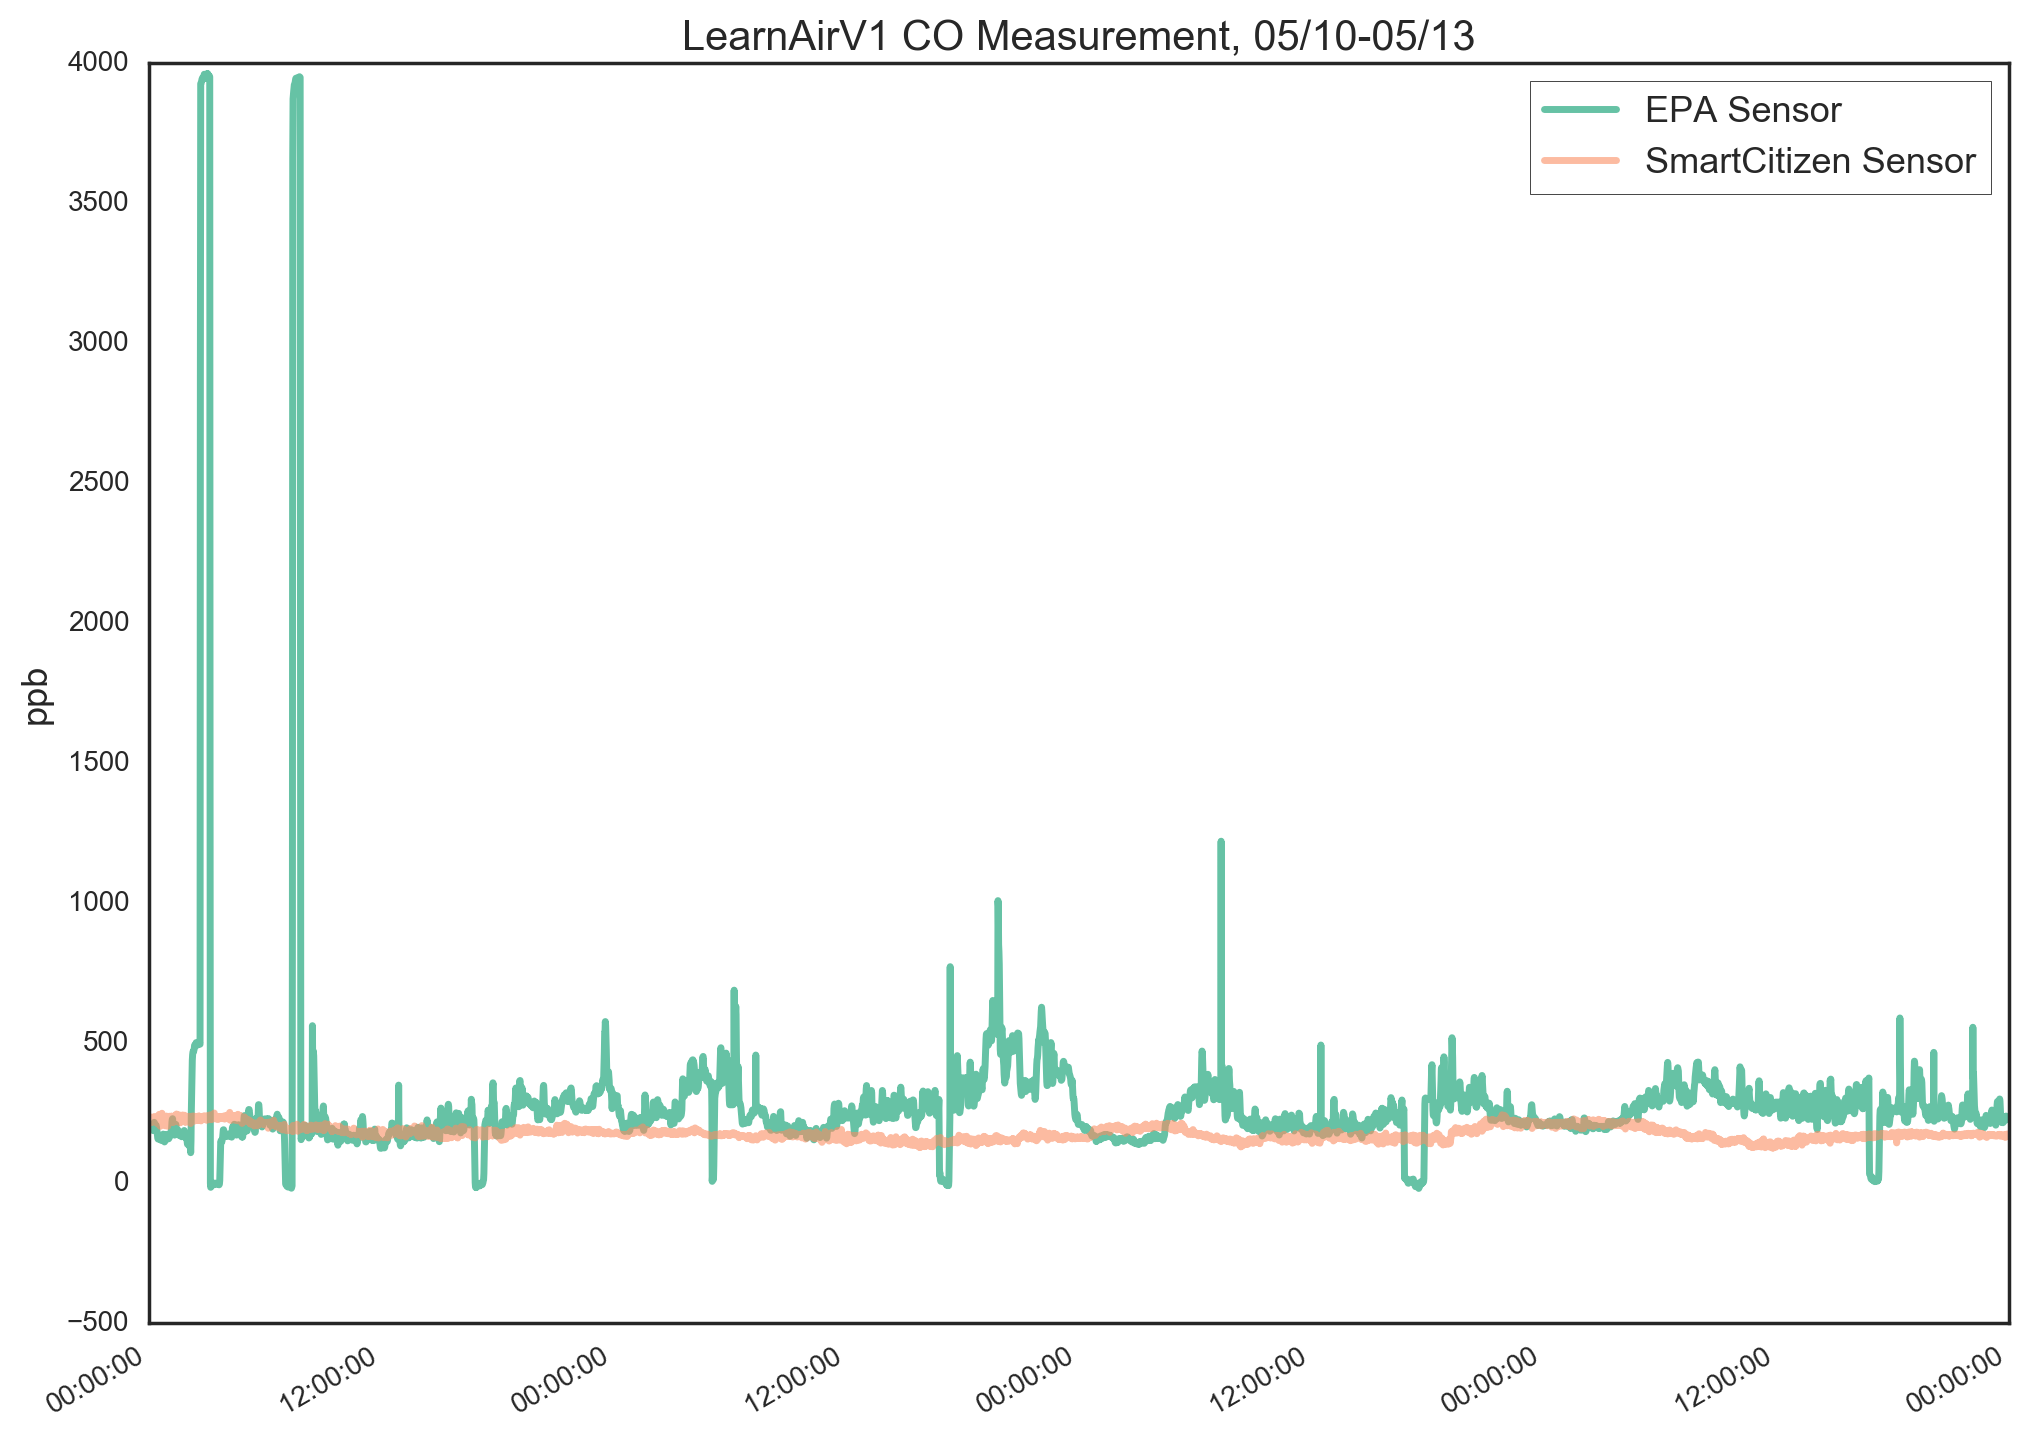
\includegraphics[width=\textwidth]{figs/co_sck_zoomed}               
 	 \caption{SmartCitizen CO Raw Data}
  	\label{fig:sck_co_raw_zoomed}
\end{figure}


\begin{figure}[htb]
 	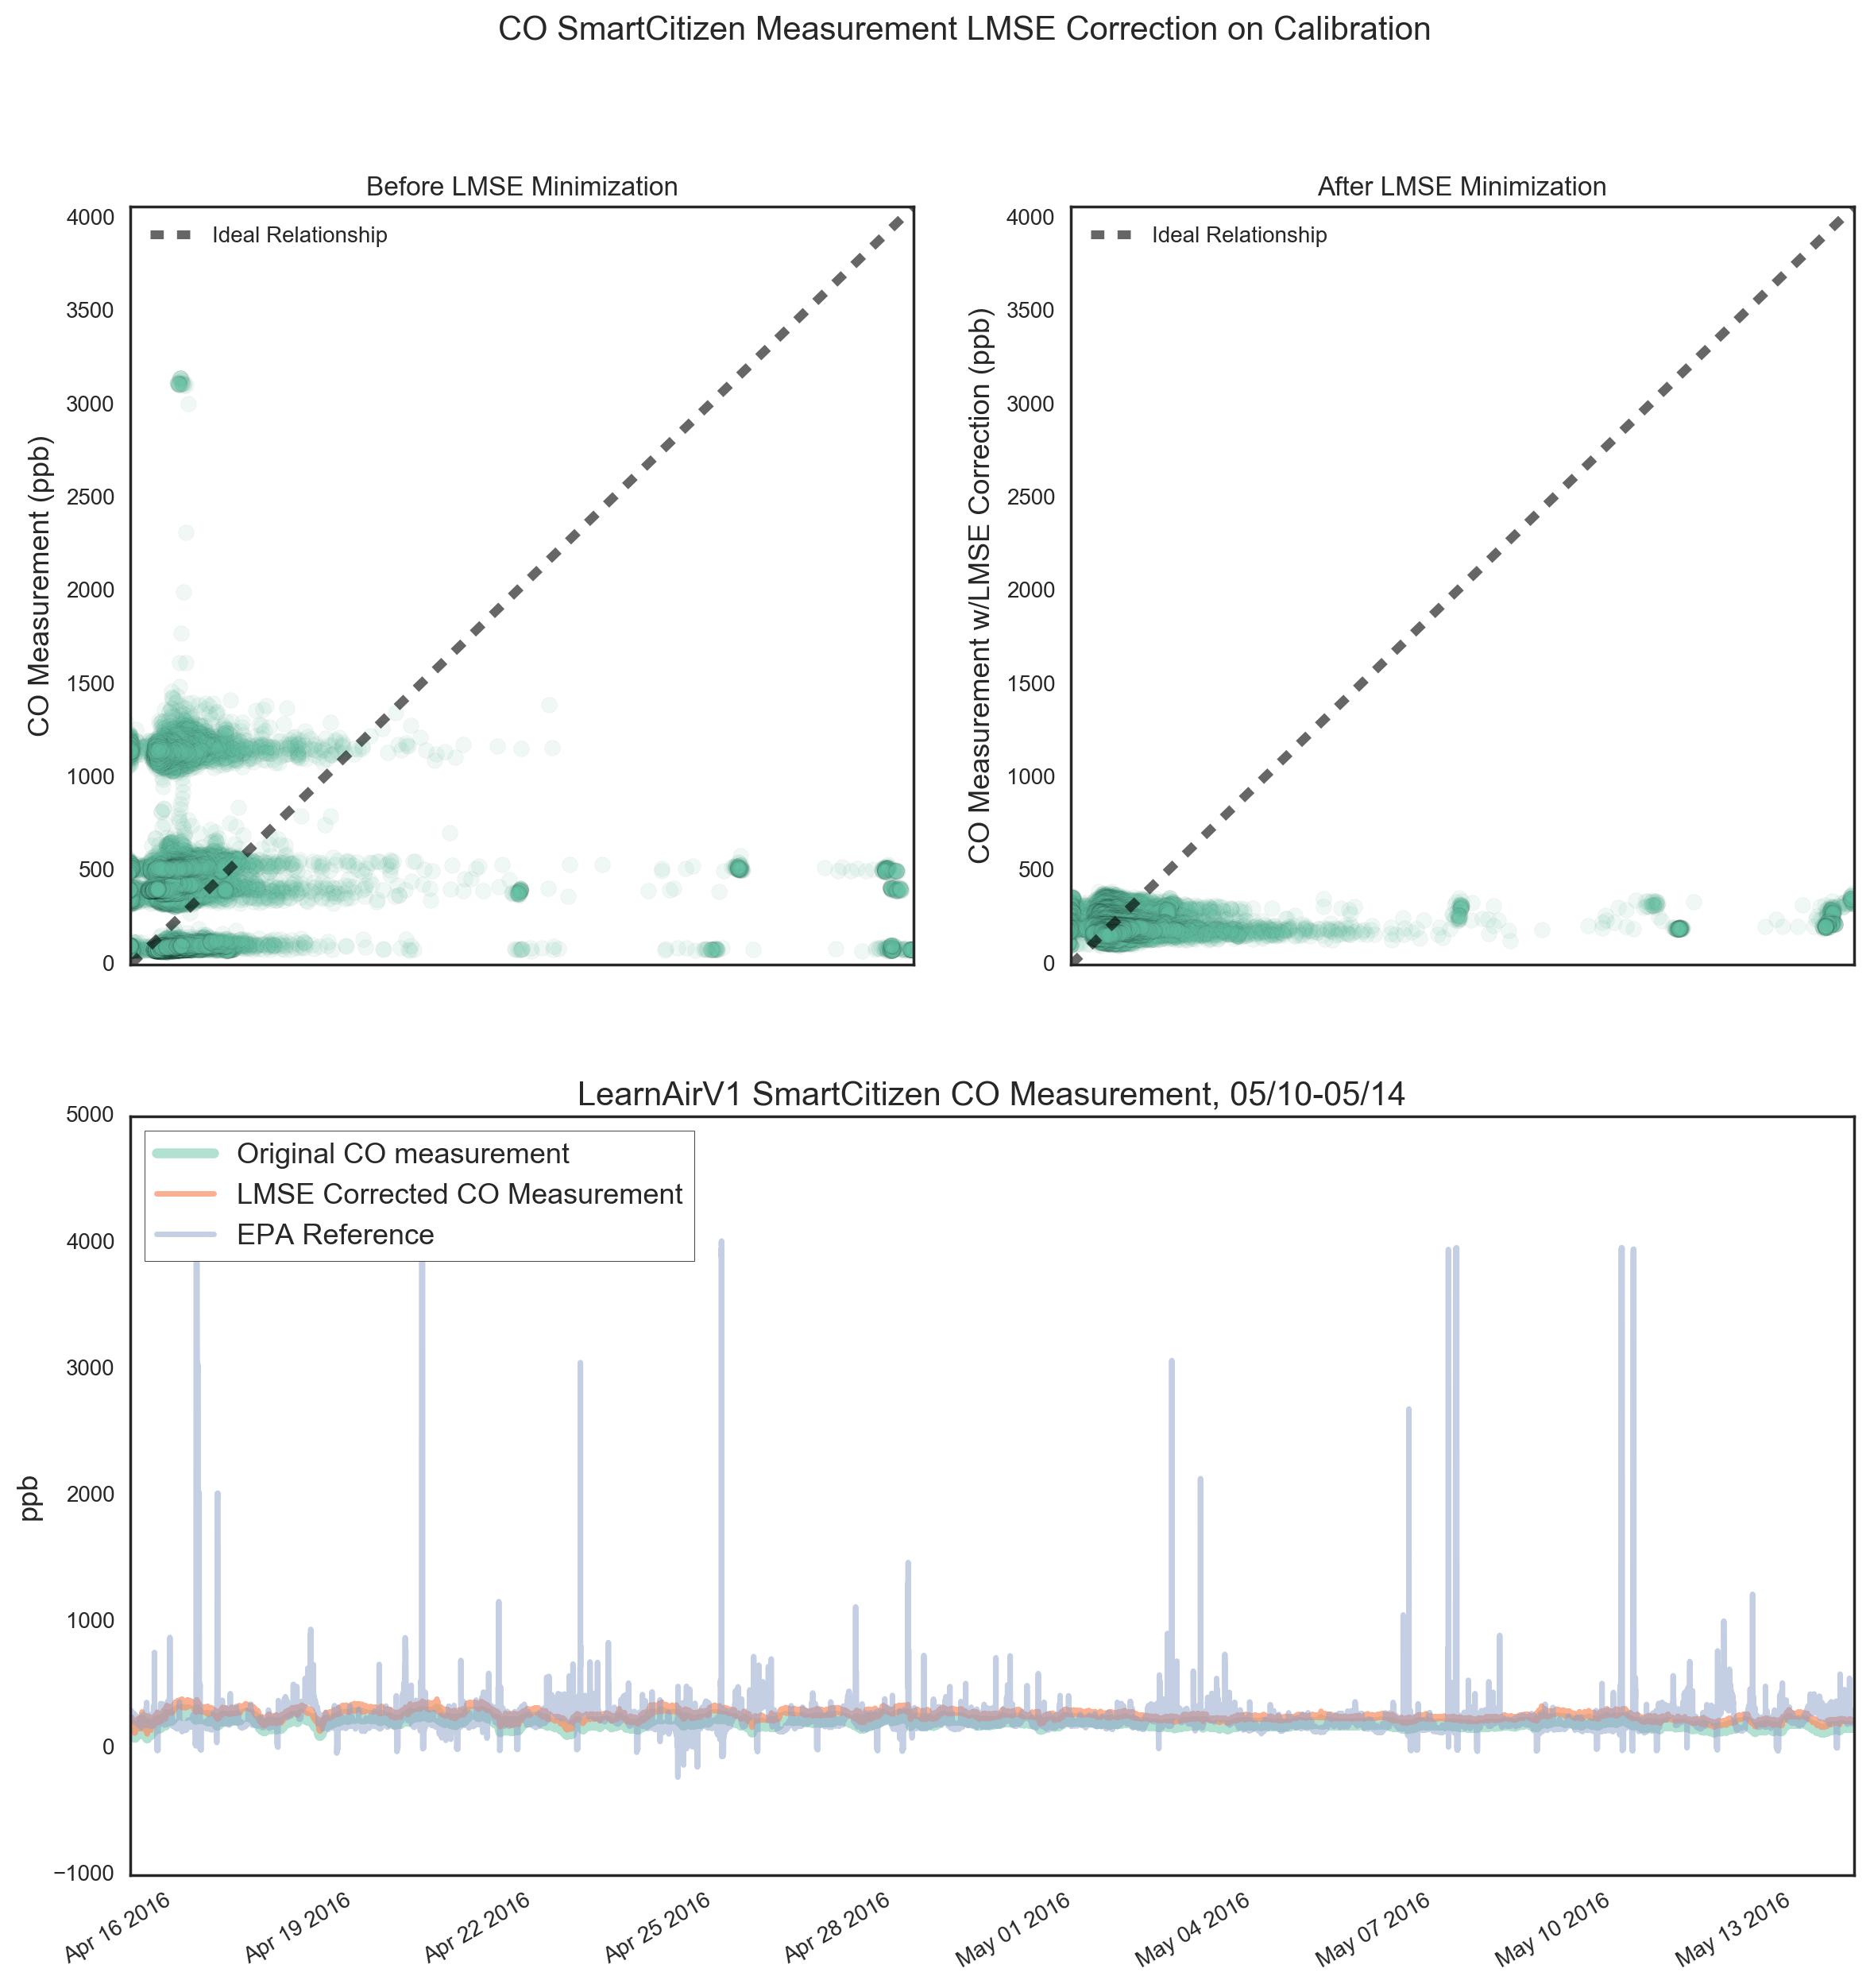
\includegraphics[width=\textwidth]{figs/sck_co_lmse}               
 	 \caption{SmartCitizen CO after LMSE Calibration}
  	\label{fig:sck_co_lmse}
\end{figure}








\subsection{Machine Learning}


\begin{figure}[htb]
 	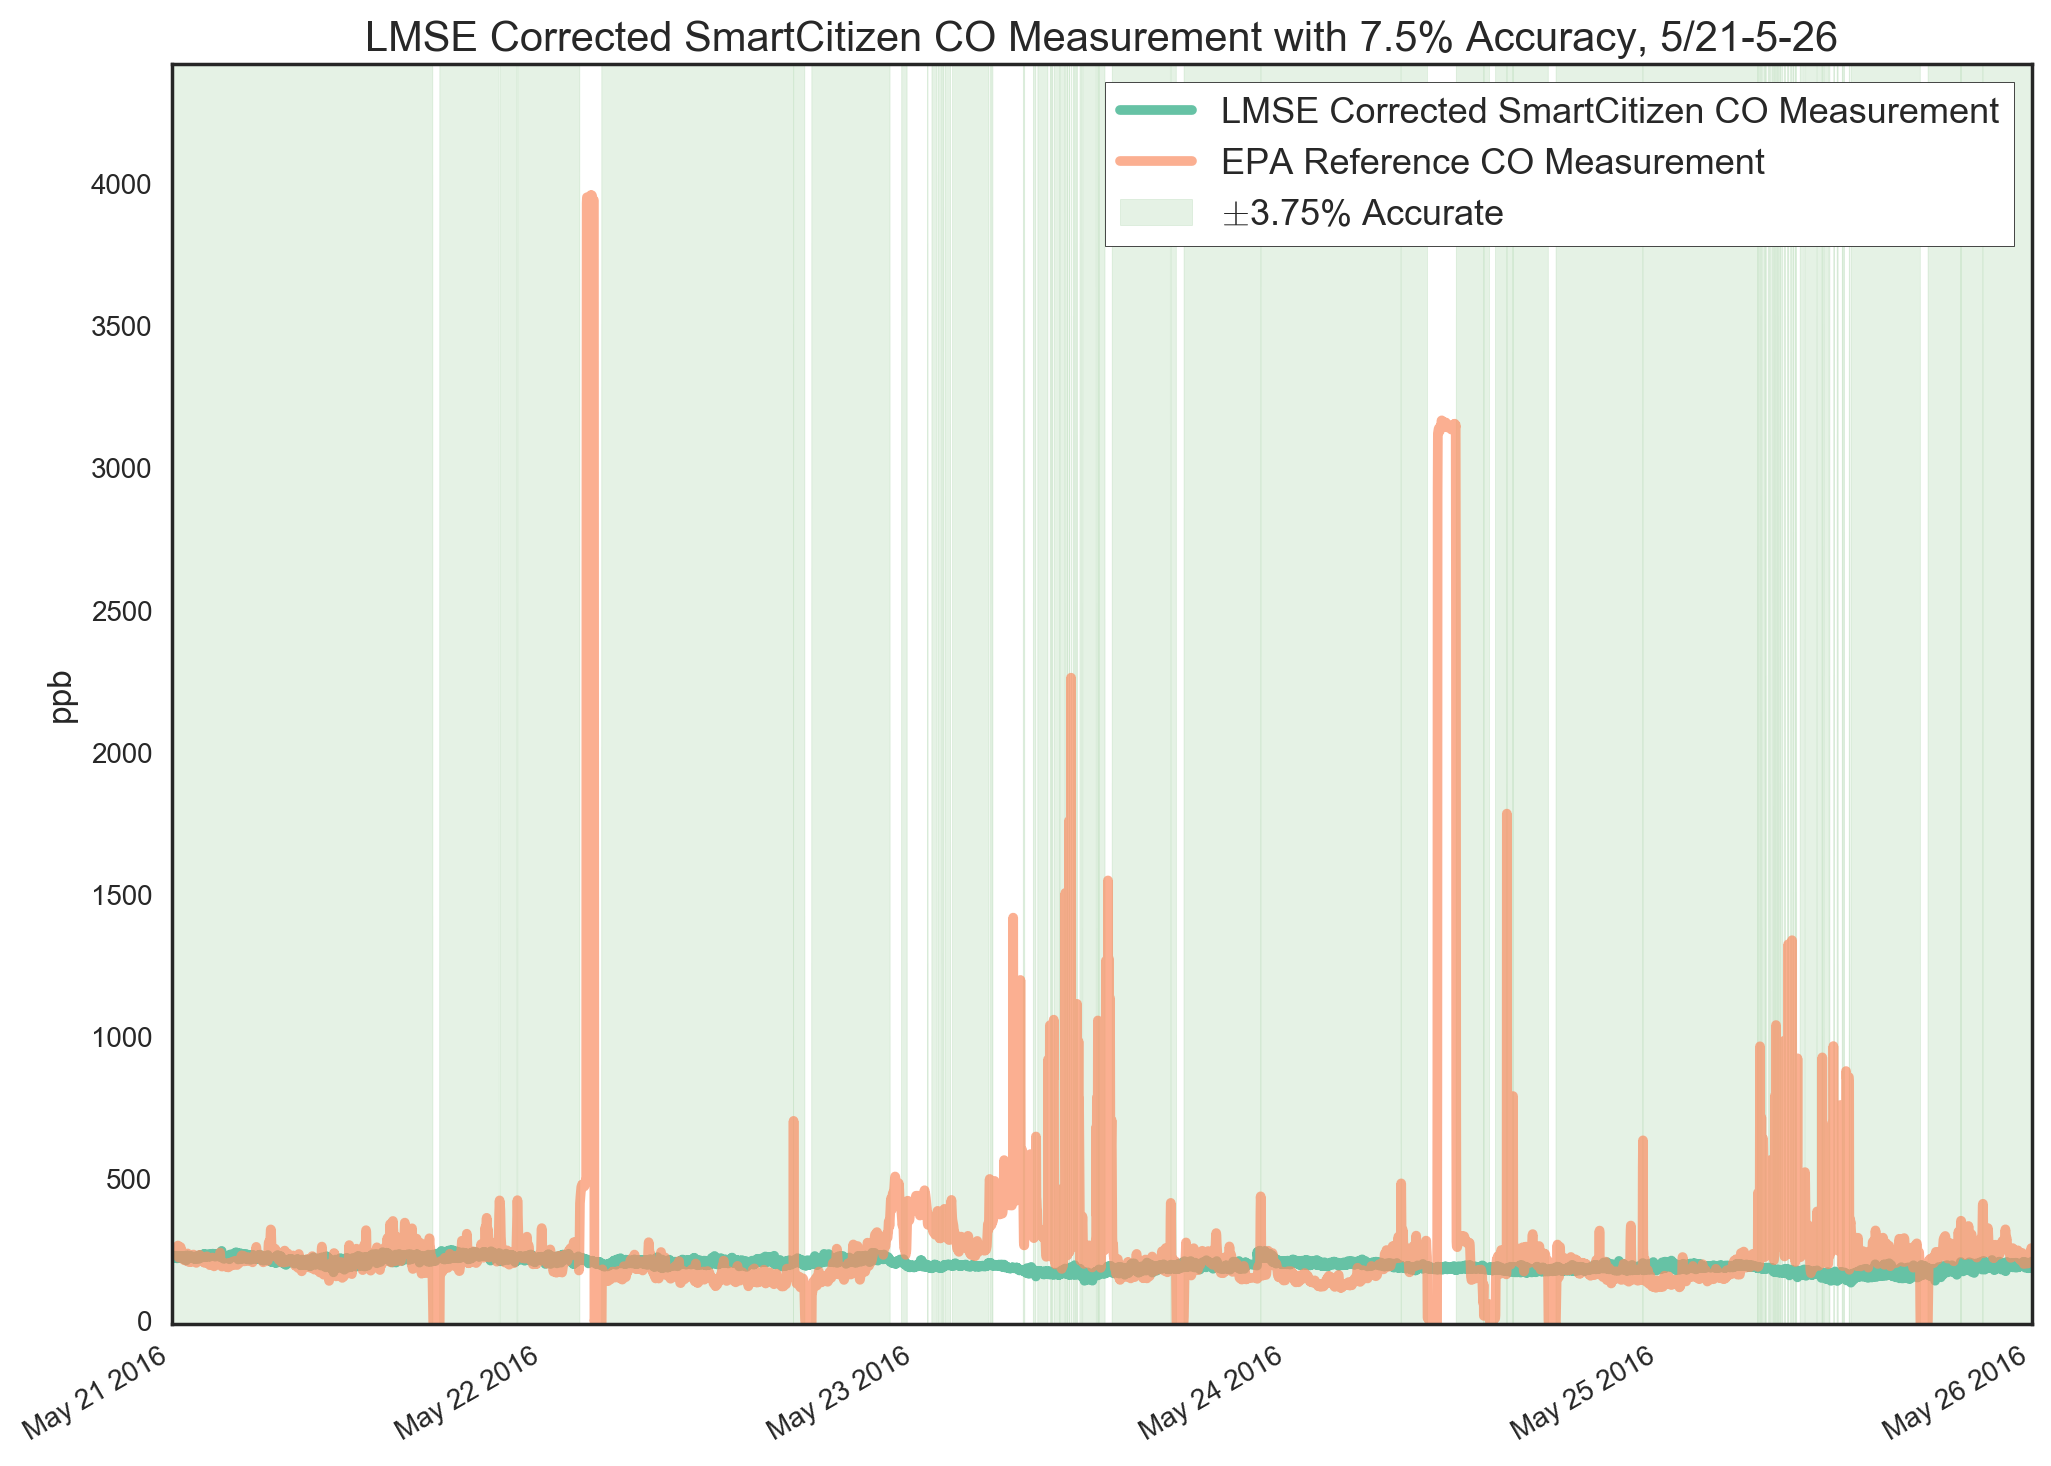
\includegraphics[width=\textwidth]{figs/sck_co_with_7p5_accuracy_zoomed}               
 	 \caption{SmartCitizen CO with 7.5\% Accuracy Threshold}
  	\label{fig:sck_co_with_7p5_accuracy_zoomed}
\end{figure}

\begin{figure}[htb]
 	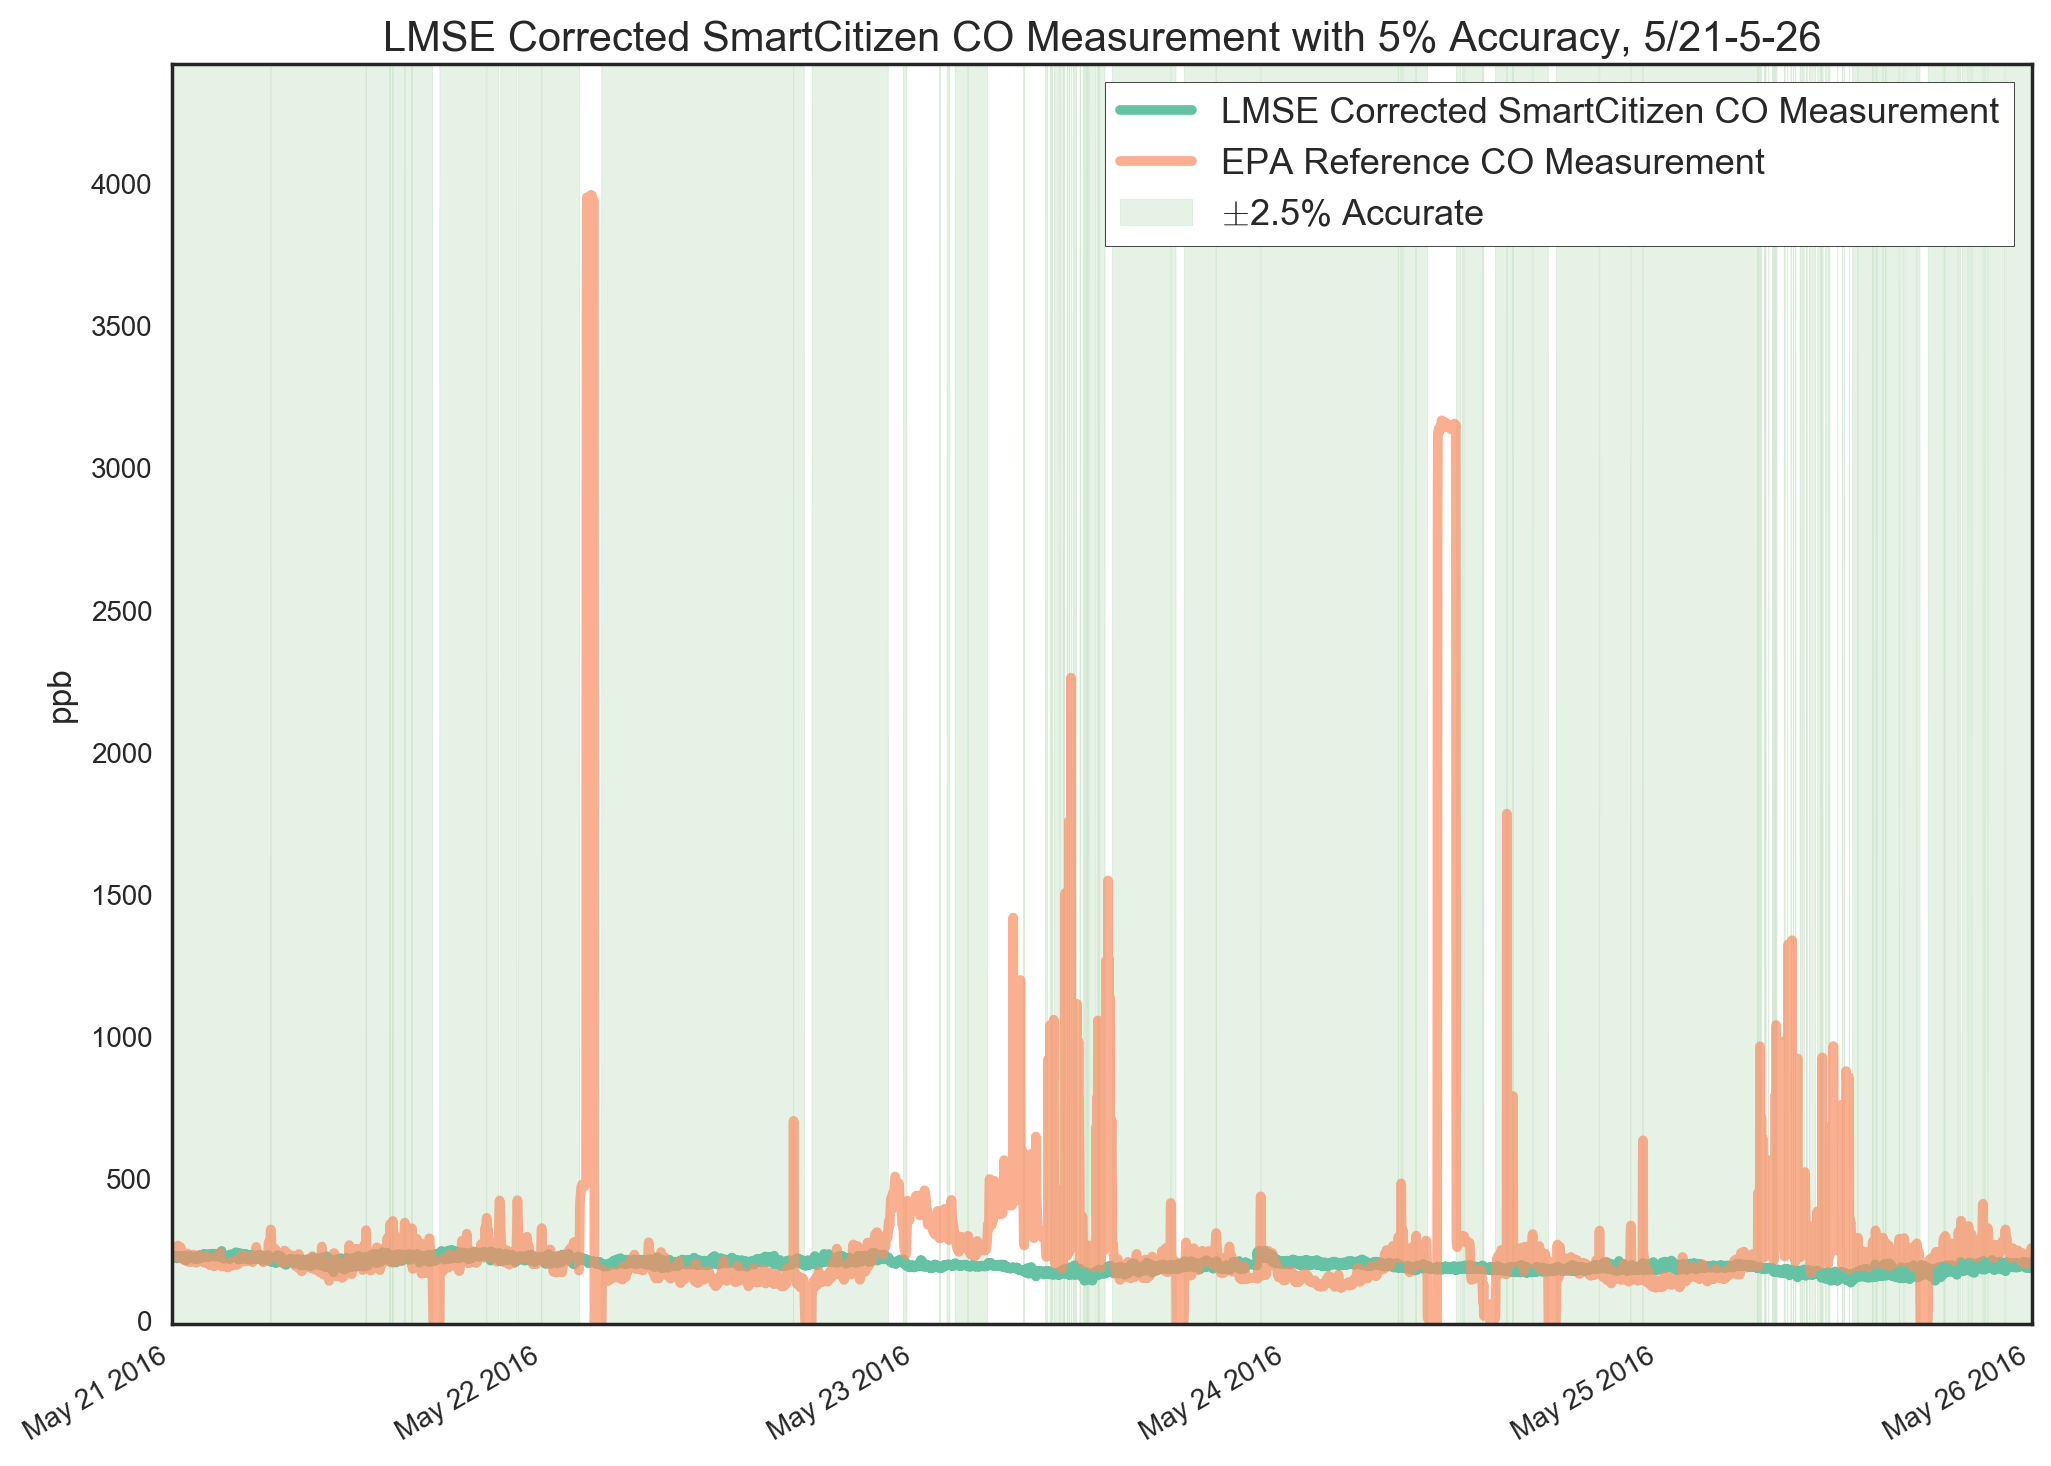
\includegraphics[width=\textwidth]{figs/sck_co_with_5_accuracy_zoomed}               
 	 \caption{SmartCitizen CO with 5\% Accuracy Threshold}
  	\label{fig:sck_co_with_5_accuracy_zoomed}
\end{figure}




parameters = {'C':[0.001, 0.1, 10, 1000], 'penalty':('L1', 'L2') }, 2 fold

===== best ROC\_AUC score 0.81902438871

===== best params {'penalty': 'L1', 'C': 10}



\begin{table}[H]
\centering
\begin{tabular}{|c|c|c|c|c|}
\toprule
\multicolumn{5}{|c|}{Error Rates for SmartCitizen CO with Logistic Regression} \\
&\multicolumn{2}{|c|}{all features} & \multicolumn{2}{|c|}{top 15 features} \\
&shuffled & chunked & shuffled & chunked \\
avg & 0.09 & 0.09 & 0.09 & 0.09 \\
min & 0.08 & 0.03 & 0.09 & 0.08 \\
max & 0.09 & 0.12 & 0.09 & 0.11 \\
\bottomrule
\end{tabular}
\label{tab:sck_co_error_rates}
\caption{Error Rates for Predicting SmartCitizen CO Accuracy with Logistic Regression}
\end{table}



\begin{table}[H]
\centering
\offinterlineskip
\hspace*{-5cm}\raisebox{-3.5cm}[0pt][0pt]{\rotatebox[origin=c]{90}{\parbox[c][0pt][c]{3cm}{\textbf{Actual Values}\\[20pt]}}}\par
\hspace*{1cm}\MyHBox[\dimexpr5.1cm+6\fboxsep\relax]{Predicted Values}\par
\hspace*{1cm}\MyHBox{0}\MyHBox{1}\par
\MyTBox{0}{197.0}{1187.4}
\MyTBox{1}{108.6}{13499.2}
}
\label{tab:as1_co_confusion}
\caption{Average SmartCitizen CO Confusion Matrix w/Shuffled K-Fold}
\end{table}


\begin{figure}[htb]
 	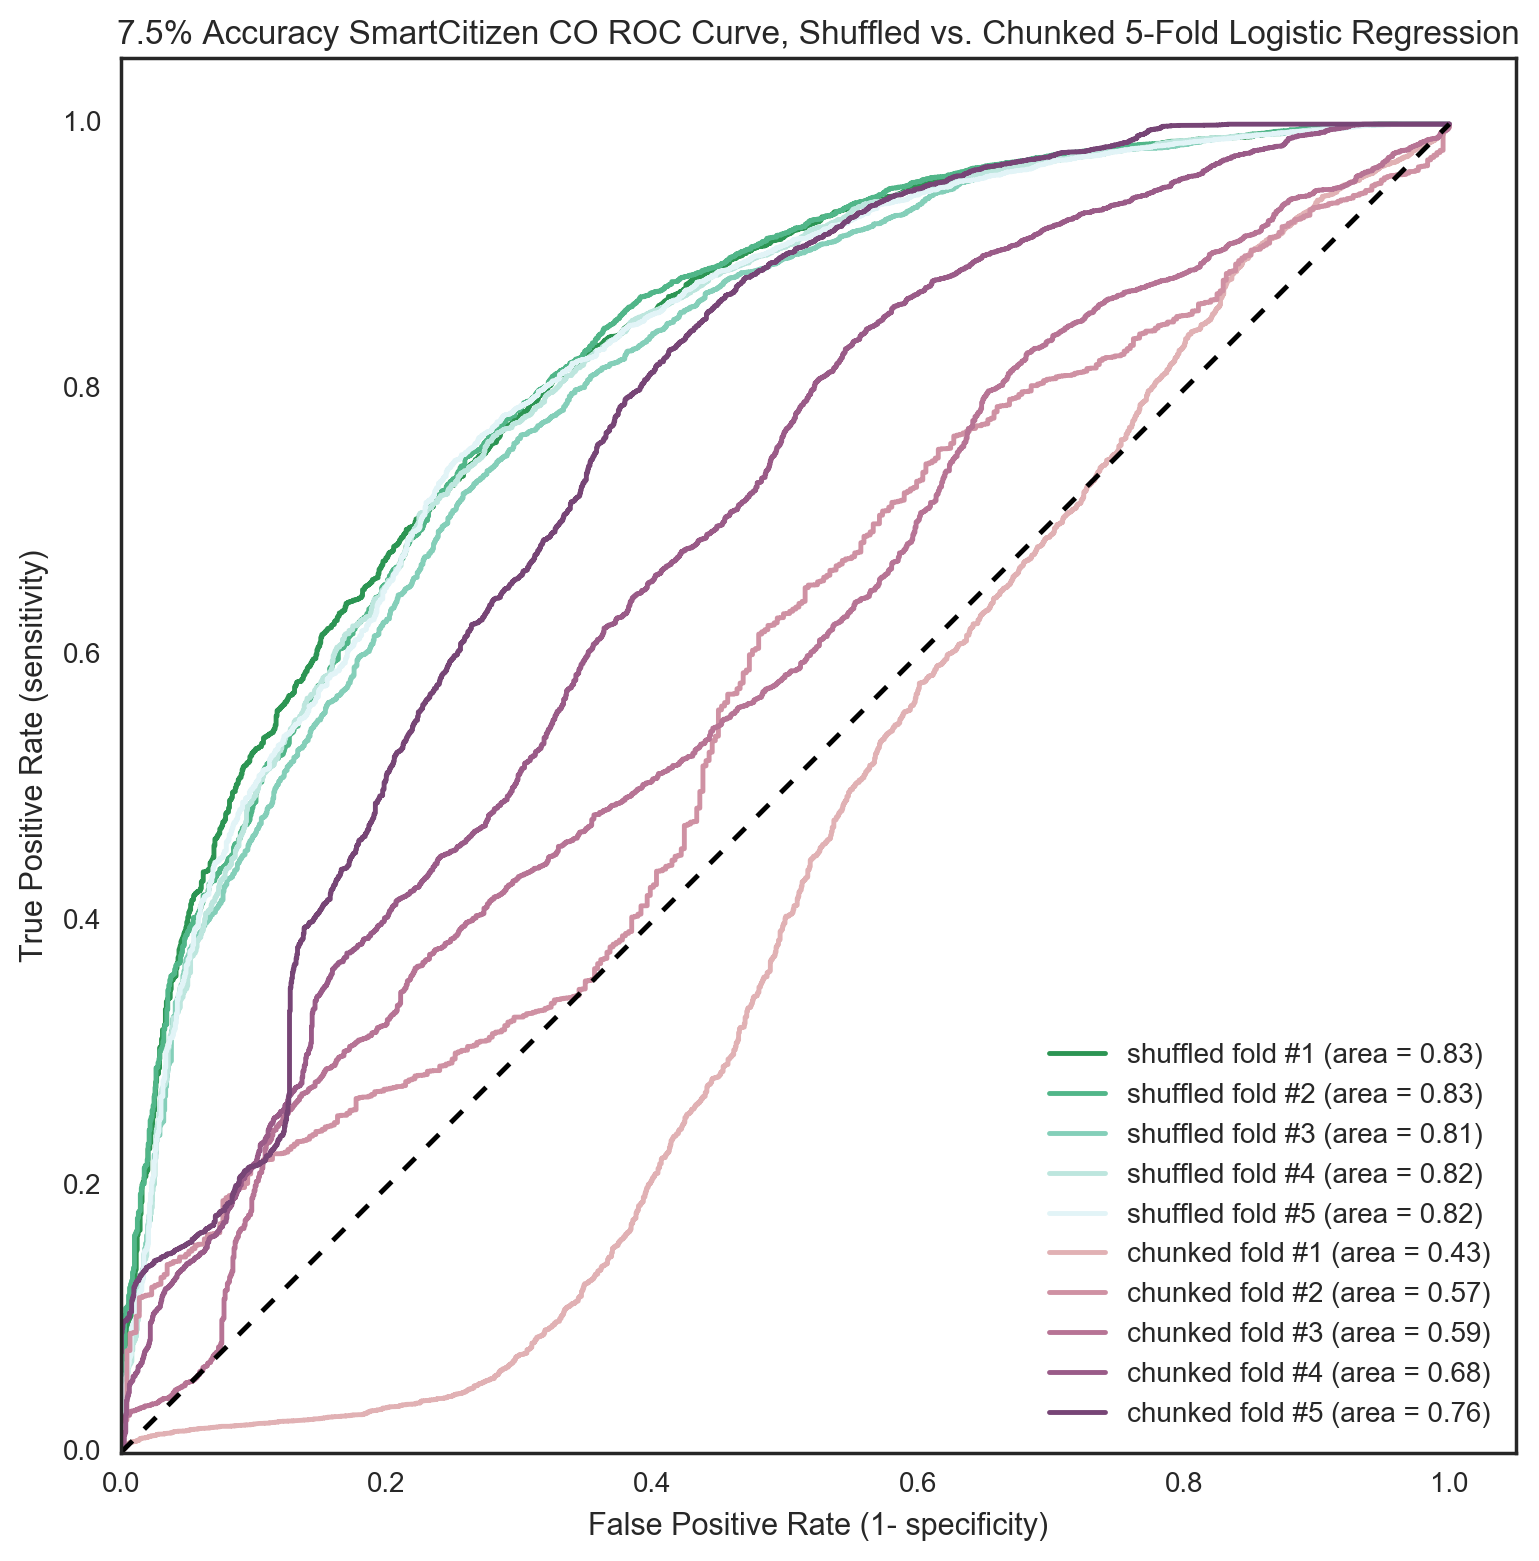
\includegraphics[width=\textwidth]{figs/sck_co_7p5_roc}               
 	 \caption{SmartCitizen CO ROC Curve}
  	\label{fig:sck_co_7p5_roc}
\end{figure}


here's text referencing the (Table \ref{tab:as1_co_randomforest_features}).

\begin{table}[H]
\centering
\begin{tabular}{lllllllll}
\\
\\
\toprule
Feature & Importance \\
\midrule
bkcarbon &  0.027481618644 \\
avg\_60\_bkcarbon &  0.0265308524121 \\
avg\_720\_bkcarbon &  0.0231734007362 \\
avg\_1440\_bkcarbon &  0.0213230536622 \\
avg\_60\_forecastio\_windSpeed &  0.0155772873357 \\
min\_since\_plugged\_in &  0.0151174982516 \\
temp\_sck\_box\_differential &  0.0148499597107 \\
avg\_60\_forecastio\_windBearing &  0.014573874136 \\
daily\_avg\_forecastio\_humidity &  0.0145367615821 \\
avg\_60\_forecastio\_dewPoint &  0.0138511147354 \\
avg\_60\_forecastio\_pressure &  0.0138476329536 \\
daily\_avg\_sck\_temperature &  0.0138353139286 \\
avg\_30\_ws &  0.0136031033823 \\
daily\_avg\_sck\_humidity &  0.0135231176757 \\
avg\_720\_lmse\_scaled\_sharpDust &  0.0132885608127 \\
\bottomrule
\end{tabular}
\label{tab:as1_co_randomforest_features}
\caption{Top 15 Features from Random Forest for SmartCitizen CO, used in Pruned Logistic Regression}
\end{table}



\begin{figure}[htb]
 	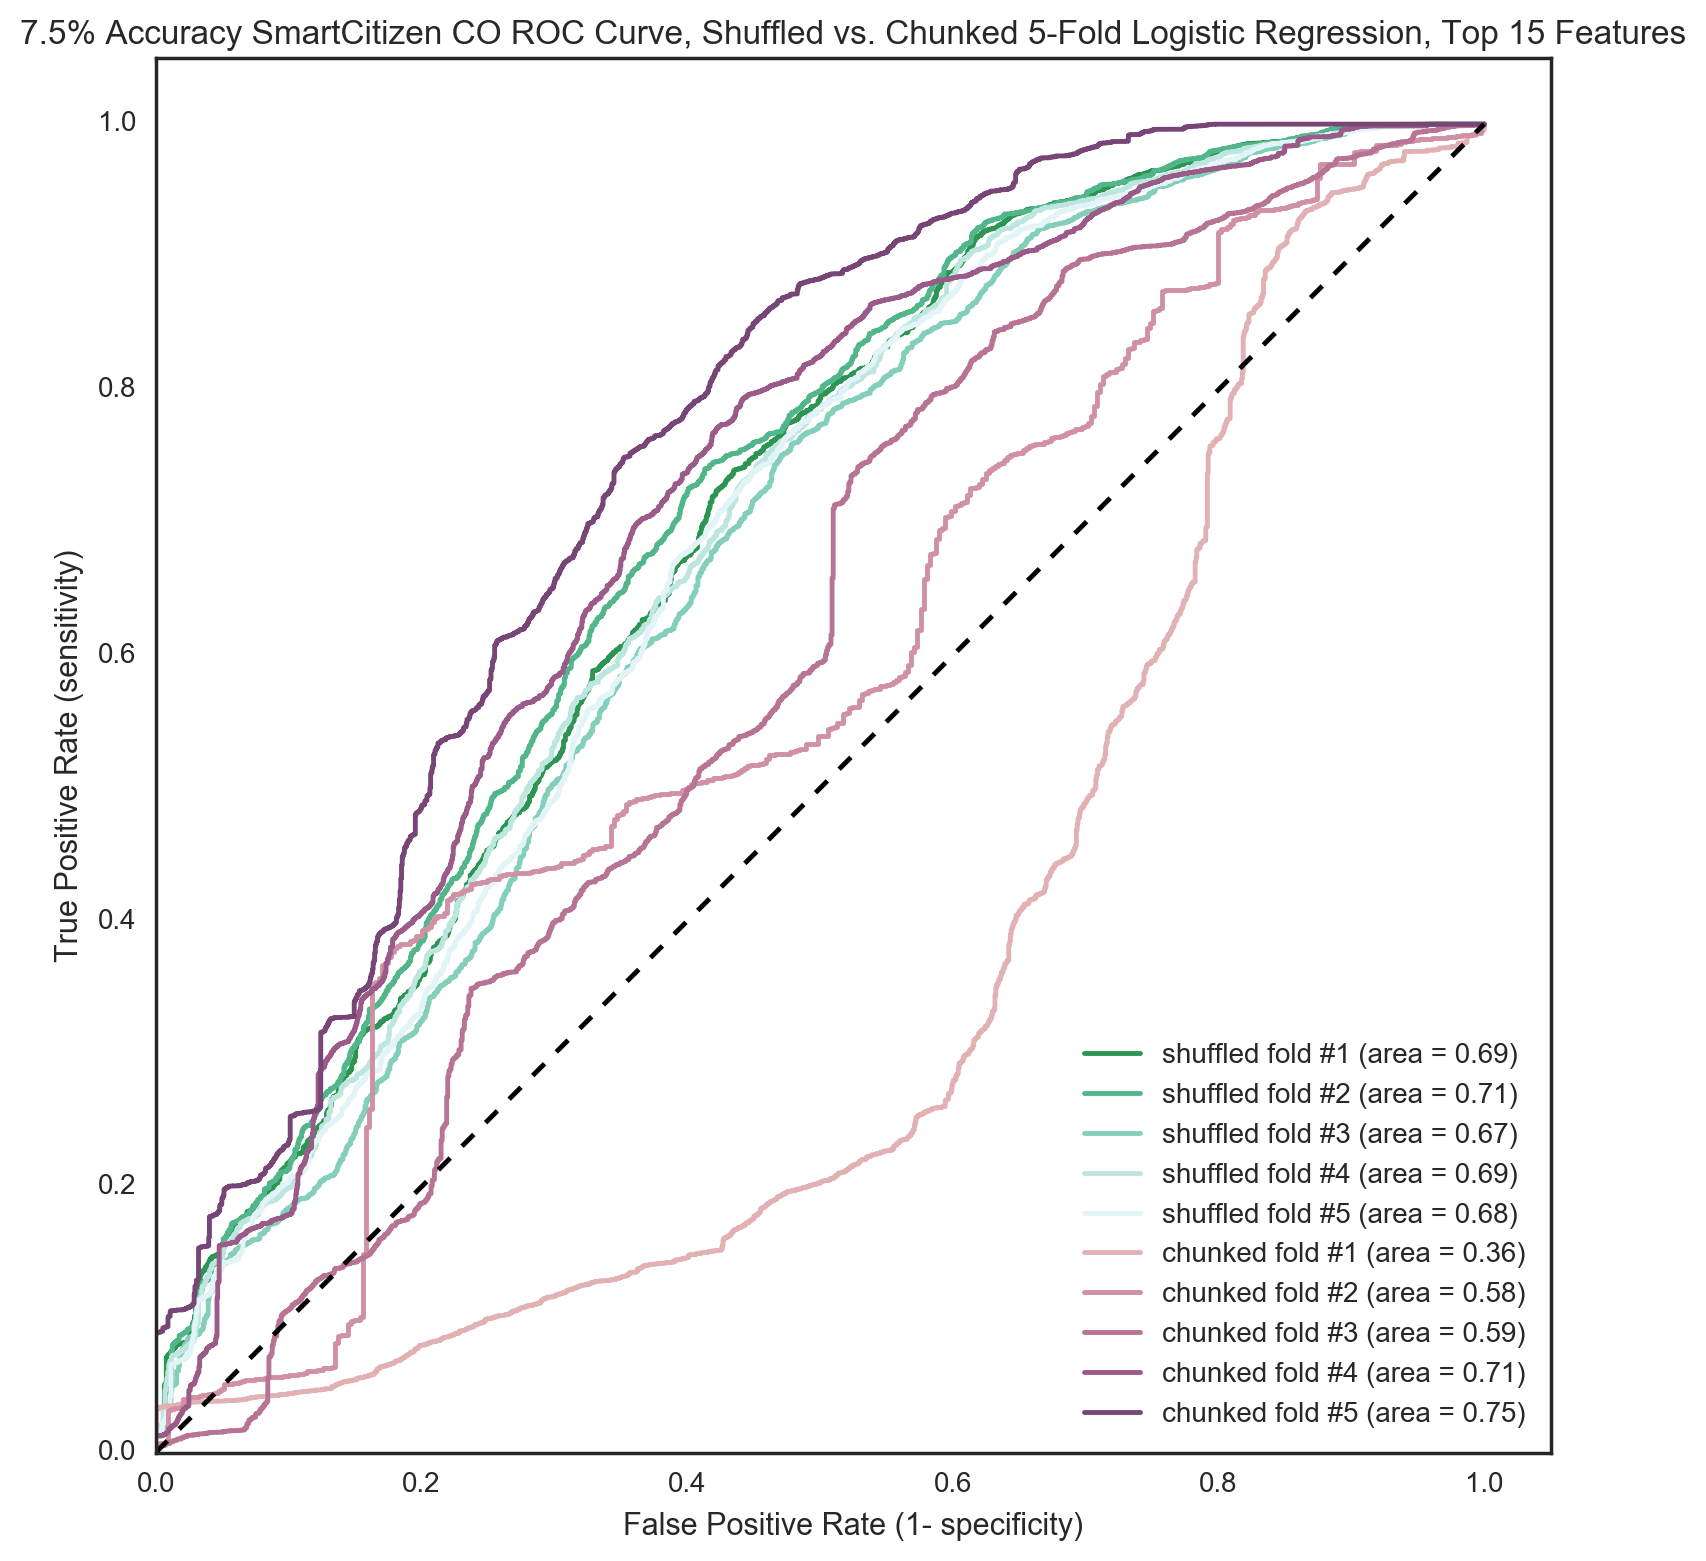
\includegraphics[width=\textwidth]{figs/sck_co_7p5_roc_pruned_features}               
 	 \caption{SmartCitizen CO ROC Using Top 15 Features}
  	\label{fig:sck_co_7p5_roc_pruned_features}
\end{figure}

\begin{figure}[htb]
 	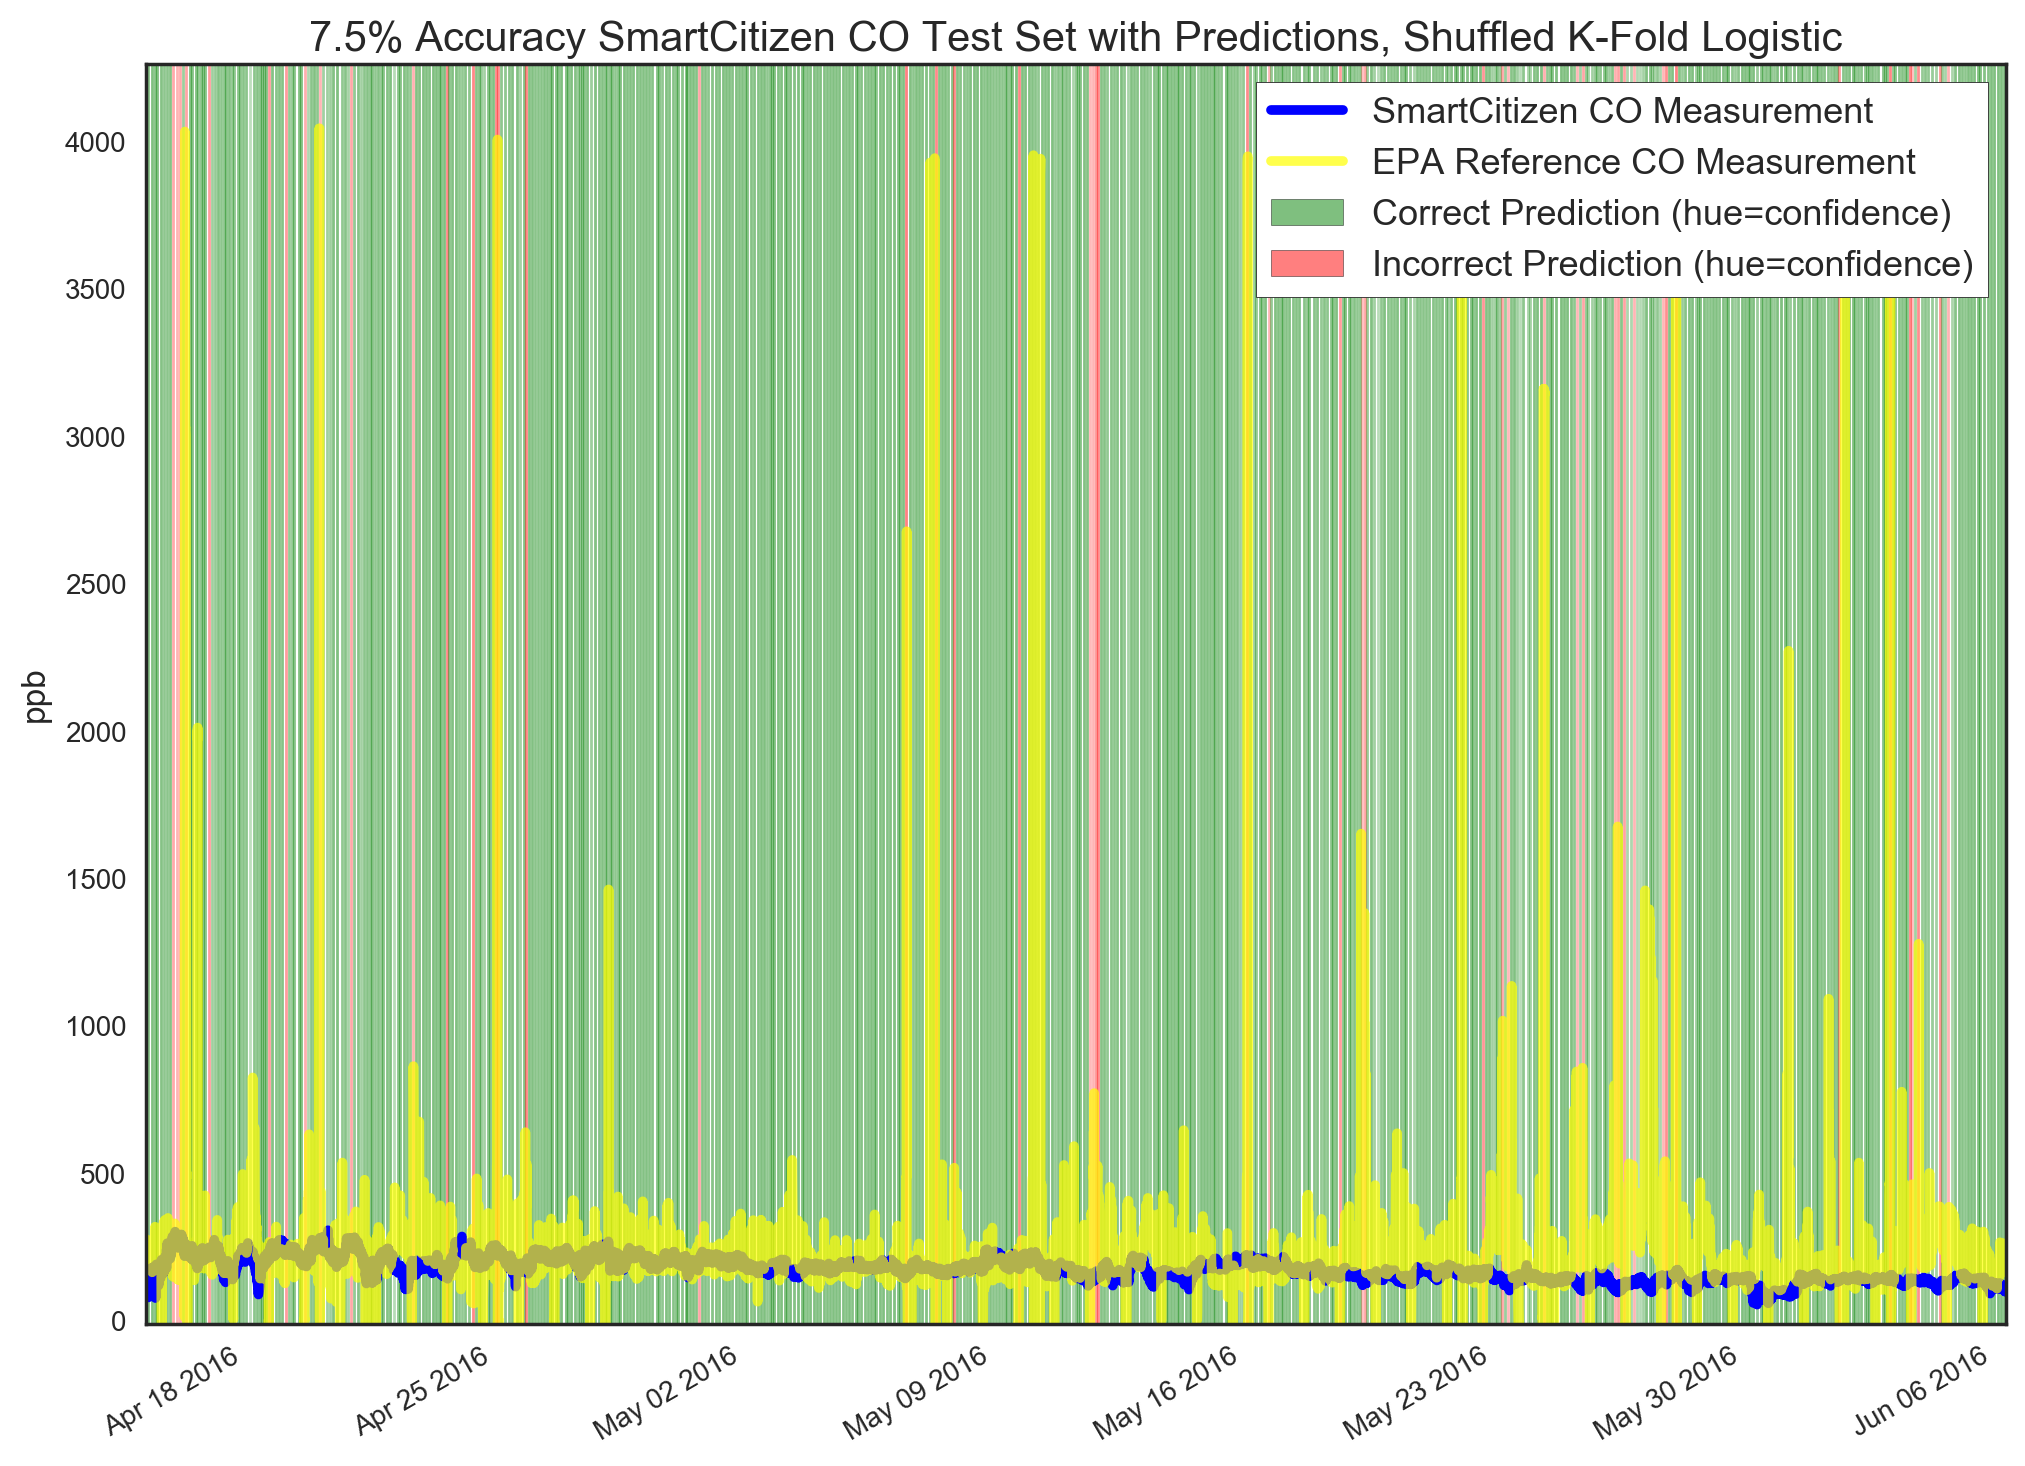
\includegraphics[width=\textwidth]{figs/sck_co_7p5_logistic_predictions}               
 	 \caption{SmartCitizen CO Prediction Accuracy}
  	\label{fig:sck_co_7p5_logistic_predictions}
\end{figure}



here's text referencing the (Table \ref{tab:as1_co_top_features}).

\begin{table}[H]
\centering
\begin{tabular}{lllllllll}
\\
\\
\toprule
     & Corr. & Lasso & Lin Reg & RF   & RFE  & Ridge & Stability & Mean \\
\midrule
bkcarbon                            & 1     & 0          & 0    & 1    & 0.58  & 0.28      & 0.93 & 0.54 \\
avg\_60\_bkcarbon                   & 0.98  & 0          & 0    & 0.25 & 0.53  & 0.15      & 0.83 & 0.39 \\
evening                             & 0.17  & 0          & 0.07 & 0.19 & 0.82  & 0.18      & 1    & 0.35 \\
avg\_1440\_bkcarbon                 & 0.57  & 0          & 0    & 0.37 & 0.53  & 0.44      & 0.54 & 0.35 \\
humidity\_box\_differential         & 0.1   & 0          & 0.01 & 0.22 & 1     & 1         & 0.02 & 0.34 \\
afternoon                           & 0.17  & 0          & 0.07 & 0    & 0.84  & 0.19      & 1    & 0.32 \\
avg\_60\_forecastio\_humidity       & 0.01  & 0          & 0.01 & 0.12 & 1     & 1         & 0    & 0.31 \\
temp\_sck\_box\_differential        & 0.09  & 0          & 0    & 0.45 & 0.84  & 0         & 0.73 & 0.3  \\
Solar Panel ( V)                    & 0.05  & 0          & 1    & 0    & 0.77  & 0         & 0    & 0.26 \\
avg\_720\_bkcarbon                  & 0.65  & 0          & 0    & 0.26 & 0.27  & 0.14      & 0.43 & 0.25 \\
forecastio\_apparentTemperature     & 0.04  & 1          & 0    & 0.03 & 0.16  & 0         & 0.43 & 0.24 \\
lmse\_avg\_30\_scaled\_arduino\_ws  & 0     & 0          & 0    & 0.05 & 0.8   & 0.03      & 0.79 & 0.24 \\
forecastio\_clear-night             & 0     & 0          & 0.08 & 0.04 & 0.91  & 0.06      & 0.51 & 0.23 \\
forecastio\_partly-cloudy-day       & 0.06  & 0          & 0.08 & 0    & 0.91  & 0         & 0.55 & 0.23 \\
forecastio\_partly-cloudy-night     & 0.01  & 0          & 0.08 & 0    & 0.89  & 0.06      & 0.54 & 0.23 \\
avg\_30\_scaled\_arduino\_ws        & 0     & 0          & 0.02 & 0.07 & 0.81  & 0         & 0.74 & 0.23 \\
Noise ( mV)                         & 0.02  & 0          & 0    & 0.11 & 0.39  & 0.02      & 0.92 & 0.21 \\
avg\_720\_lmse\_scaled\_sharpDust   & 0.03  & 0          & 0    & 0.15 & 0.55  & 0.22      & 0.52 & 0.21 \\
derivative\_avg\_720\_bkcarbon      & 0     & 0          & 0    & 0.12 & 0.63  & 0.25      & 0.45 & 0.21 \\
daily\_avg\_sck\_humidity           & 0.07  & 0          & 0    & 0.18 & 0.59  & 0.17      & 0.4  & 0.2  \\
derivative\_avg\_360\_lmse\_as\_no2 & 0     & 0          & 0    & 0.11 & 0.55  & 0.73      & 0    & 0.2  \\
derivative\_avg\_1440\_bkcarbon     & 0.02  & 0          & 0    & 0.14 & 0.64  & 0.02      & 0.58 & 0.2  \\
evening\_rush                       & 0.13  & 0          & 0    & 0.04 & 0.49  & 0.1       & 0.54 & 0.19 \\
avg\_60\_forecastio\_pressure       & 0.07  & 0          & 0    & 0.26 & 0.41  & 0.01      & 0.6  & 0.19 \\
\bottomrule
\end{tabular}
\label{tab:as1_co_top_features}
\caption{Top Features for Predicting SmartCitizen CO}
\end{table}


\FloatBarrier

\section{SmartCitizen NO2}
One SmartCitizen NO2 sensor was tested against the EPA reference.  Like the SmartCitizen CO test, it was 1 month old at the time of installation, and ran for 52 days (from 4/15 - 6/6 2016) with two ~40 minute service interruptions.  It gave 74,961 samples of minute resolution data.

\begin{marginfigure}
 	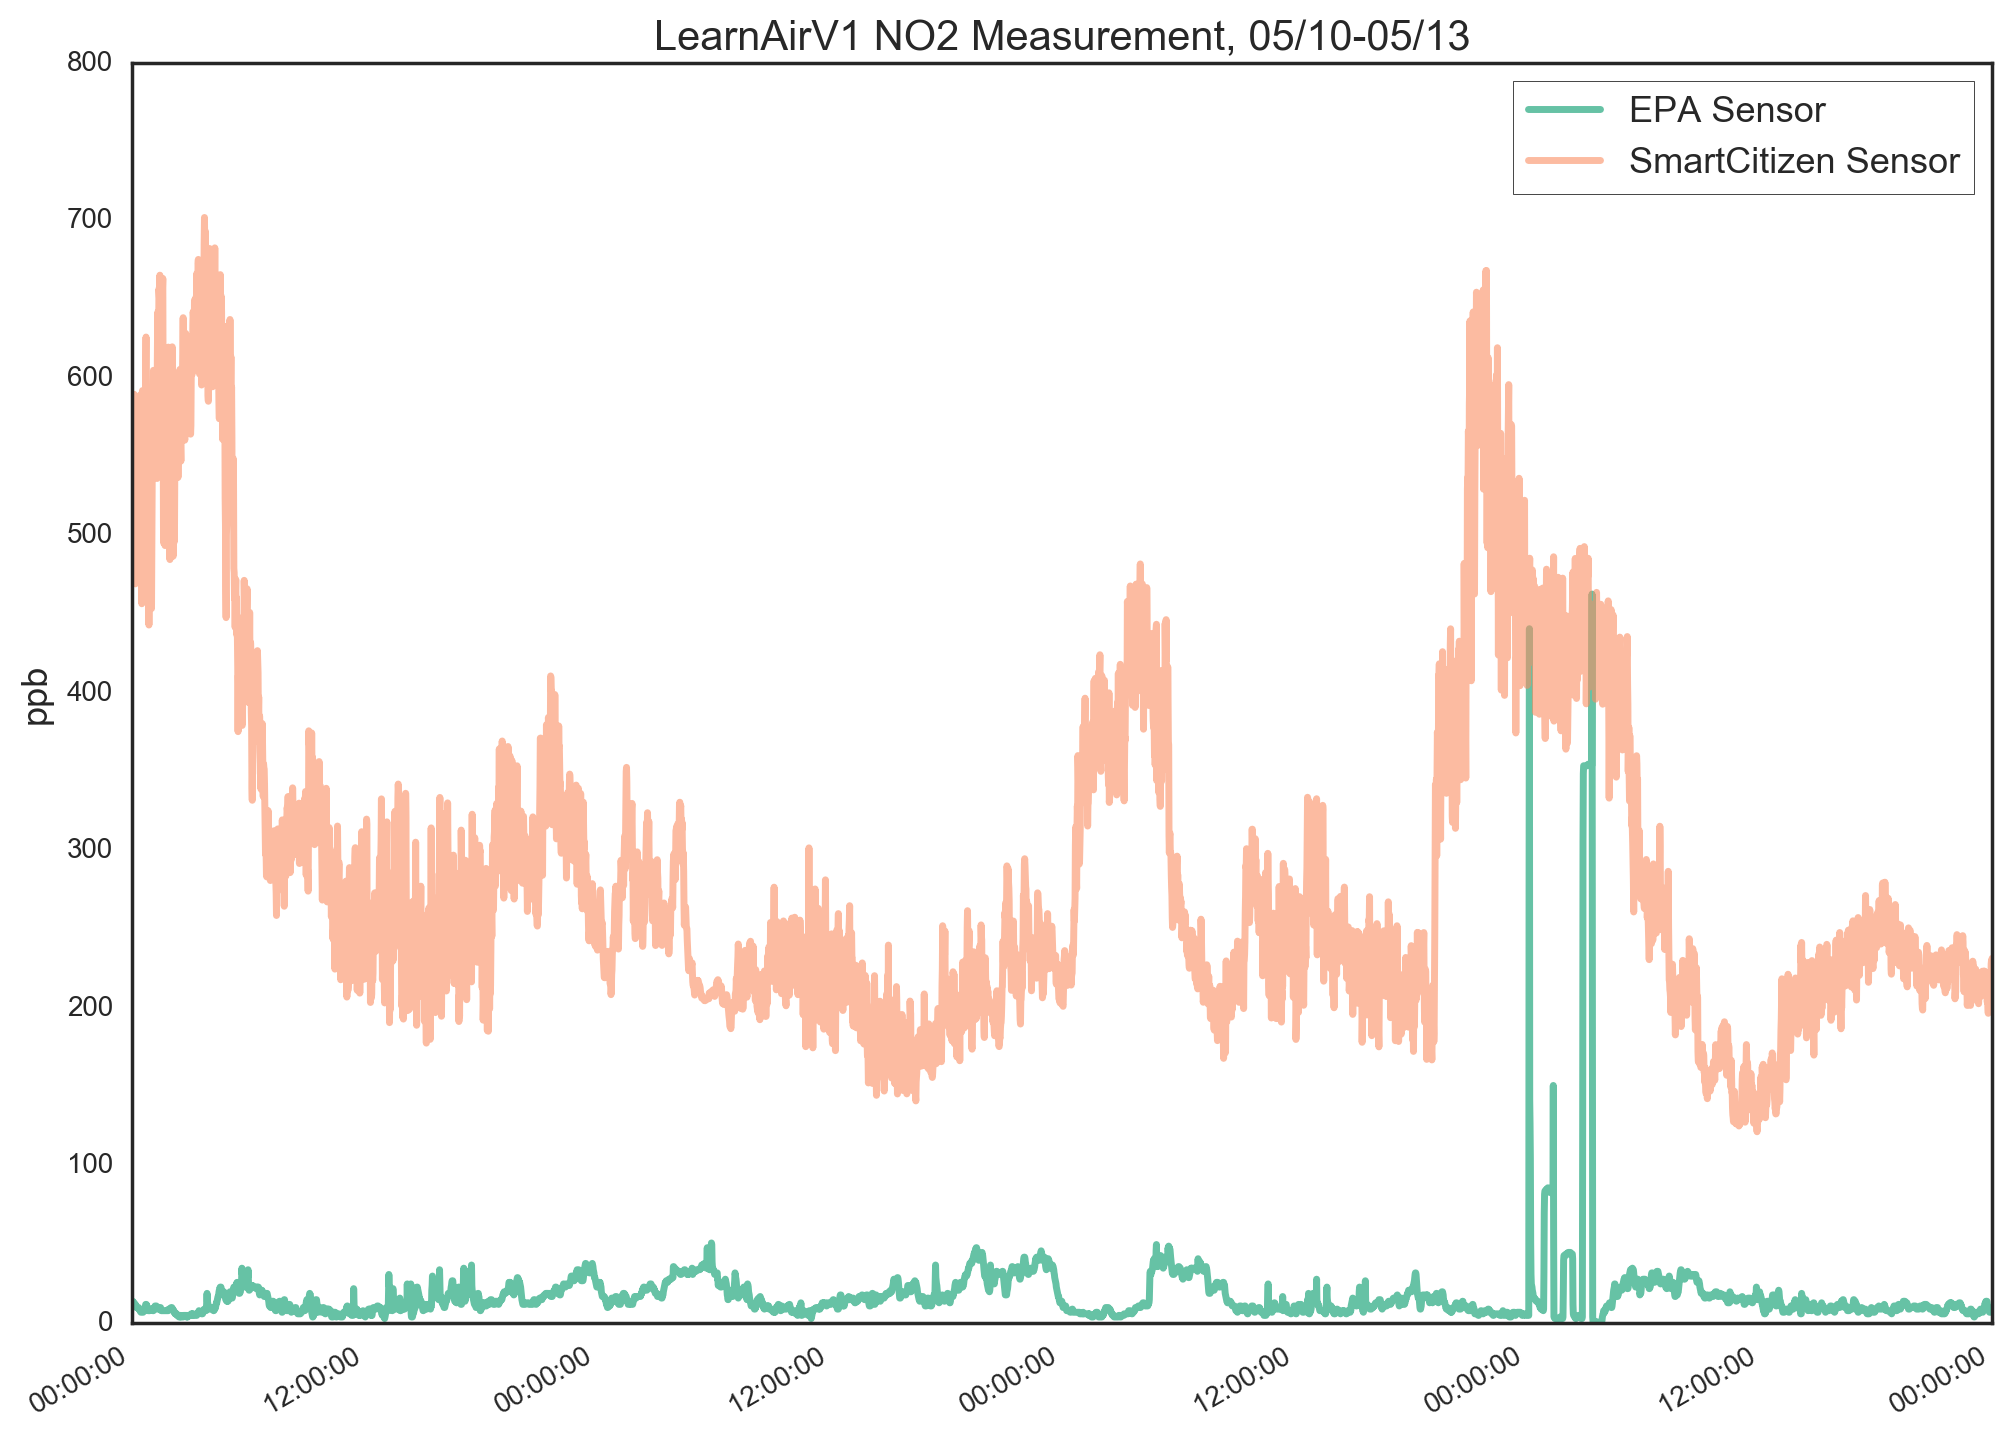
\includegraphics[width=\textwidth]{figs/no2_sck_zoomed}               
 	 \caption{SmartCitizen NO2 Raw Data}
  	\label{fig:sck_no2_raw_zoomed}
\end{marginfigure}

\subsection{Pre-processing}

\enlargethispage{\baselineskip}

Like the SmartCitizen CO data, the NO2 sensor comes uncalibrated, as a mV value.  The first step was to run a bounded LMSE minimization on the data in order to scale and offset it appropriately to match the real data.  You can see the final result of such a scaling in Figure \ref{fig:sck_no2_with_10_accuracy_zoomed}.  Once again, the LMSE minimization scaled the sensor values down to a minimal amount of variation.  This suggests that the sensor data itself is relatively useless in this context, which is relatively unsurprising given its working range and the near constant <1 ppm exposure.  This agrees with spurious test findings for three SmartCitizen NO2 sensors tested by SCAQMD.   


\subsection{Machine Learning}

This case is similar to the SmartCitizen CO sensor, as machine learning will tell us nothing of the sensor's accuracy.  It reduces to a different problem, instead-- predicting NO2 transients and elevated levels based on metrological and other sensor data. 

\begin{figure}[htb]
 	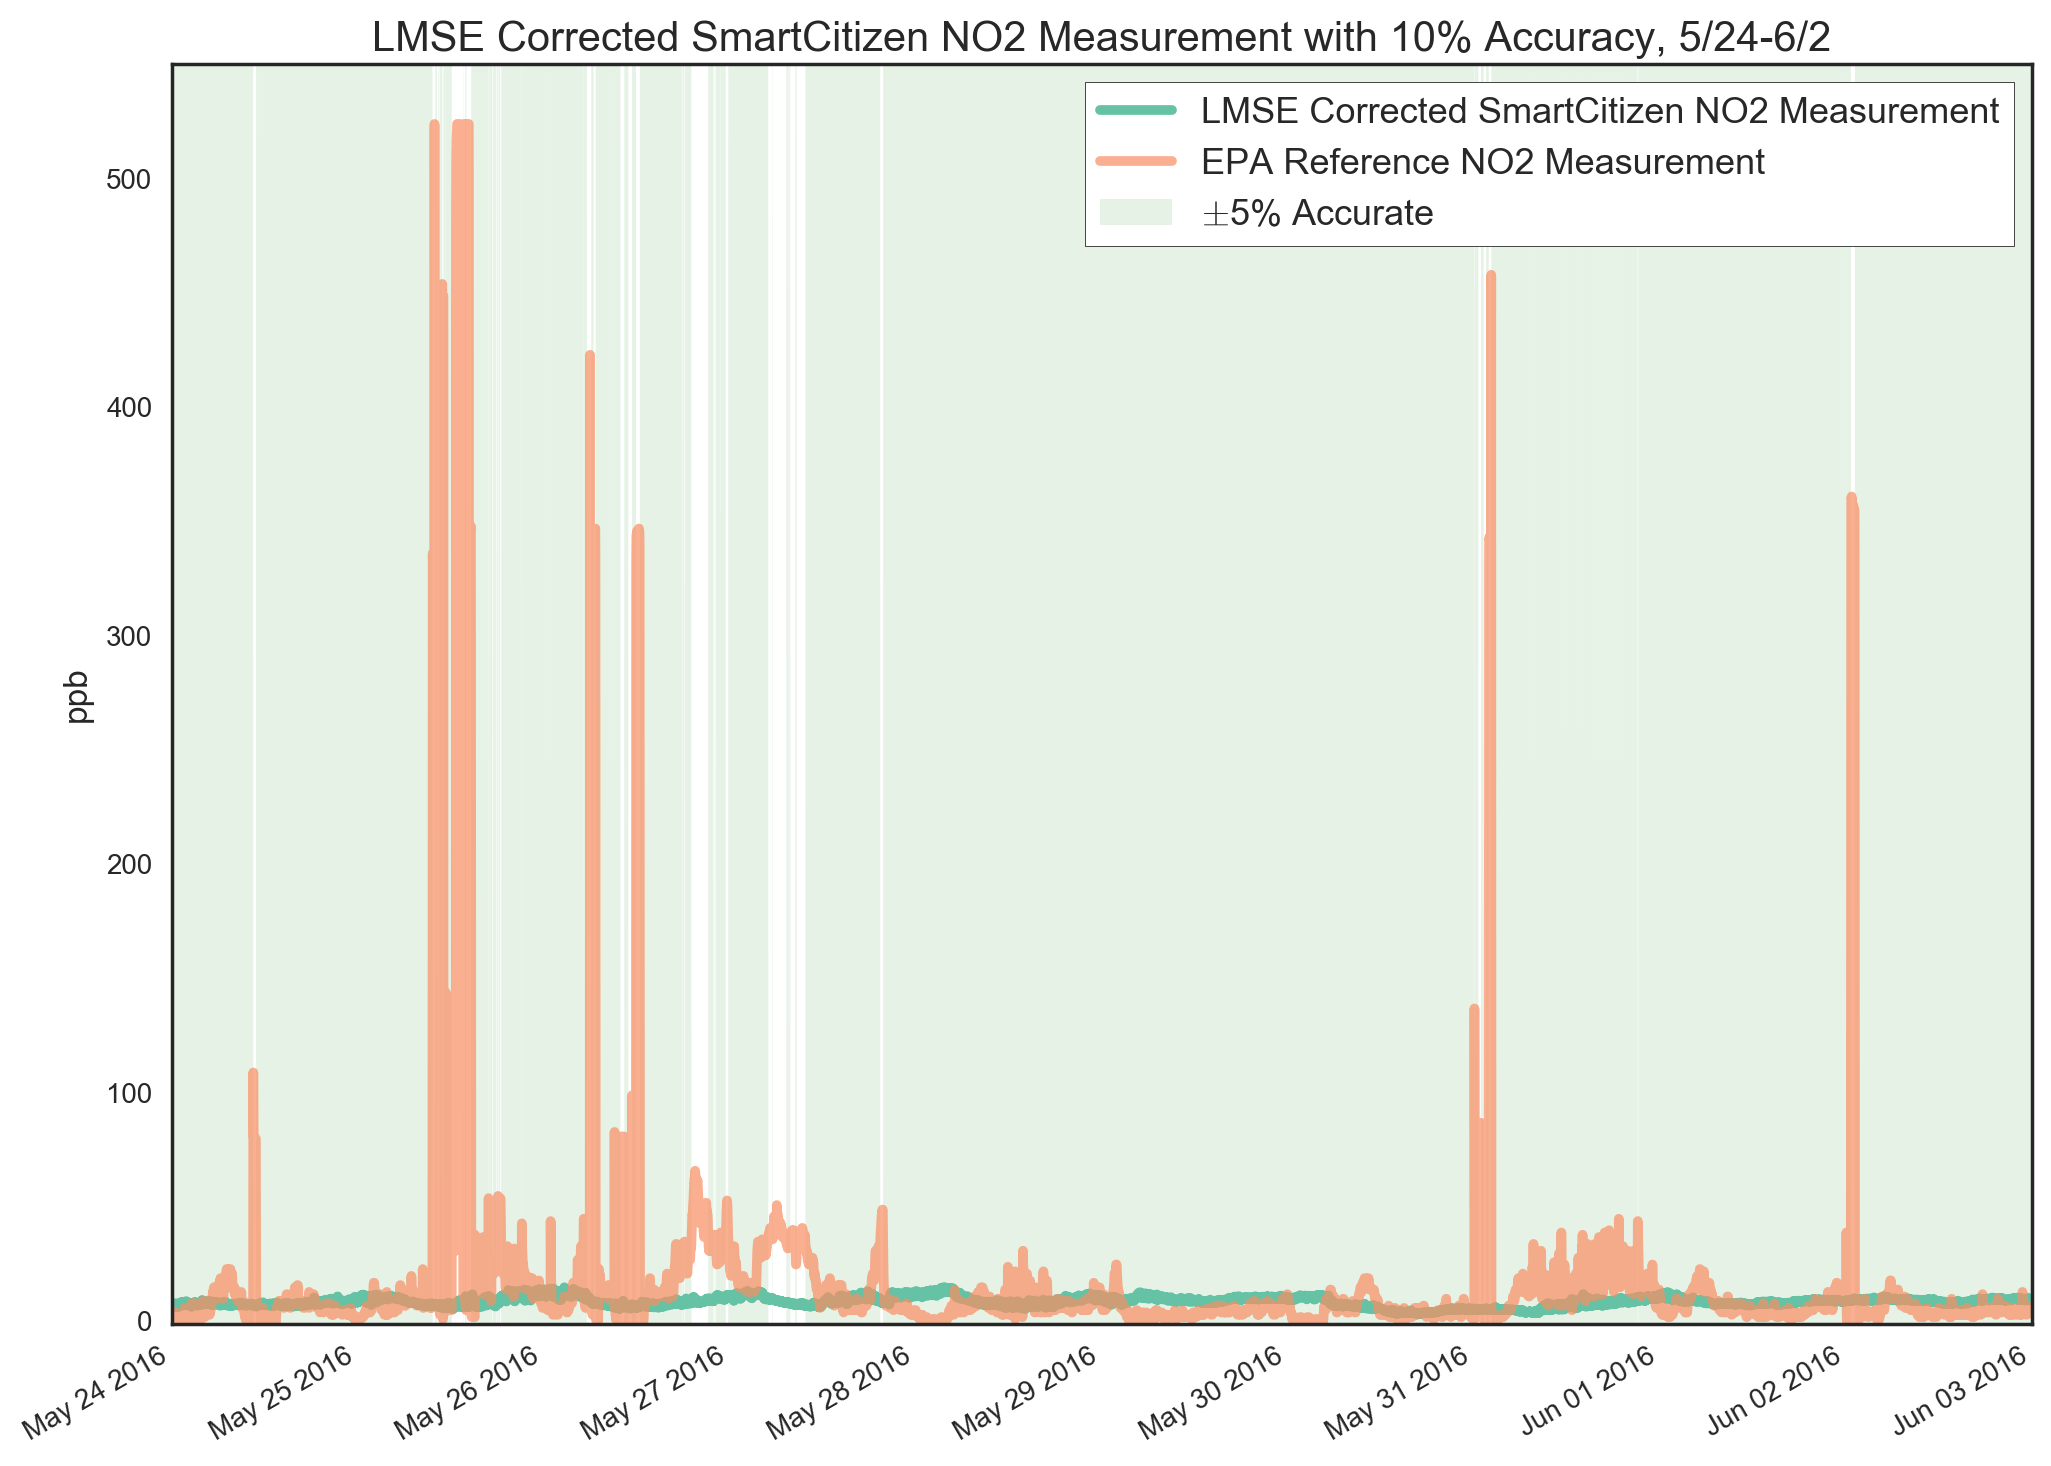
\includegraphics[width=\textwidth]{figs/sck_no2_with_10_accuracy_zoomed}               
 	 \caption{SmartCitizen NO2 with 10\% Accuracy Threshold}
  	\label{fig:sck_no2_with_10_accuracy_zoomed}
\end{figure}



The threshold for accuracy was set at 10\% (or $\pm$5\%) of the full range of values detected for the actual NO2 levels, ~50 ppb ($\pm$25 ppb).   Figure \ref{fig:sck_no2_with_10_accuracy_zoomed} shows the Smart Citizen values against the reference, with `accurate' measurements highlighted with a green background.  The `inaccurate' readings are the peaks and large diversions from the baseline.

As with all of the machine learning models, scikit learn was used to conduct a parameterized search for the optimal logistic regression was conducted using parameters C = [0.001, 0.1, 10, 1000] and penalty-type=['L1', 'L2'] with a 2-fold cross-validation.  An L1 penalty and C=1000 regularization term gave the best ROC\_AUC score of 0.91.  

\begin{table}[]
\centering
\begin{tabular}{|c|c|c|c|c|}
\toprule
\multicolumn{5}{|c|}{Error Rates for SmartCitizen NO2 with Logistic Regression} \\
&\multicolumn{2}{|c|}{all features} & \multicolumn{2}{|c|}{top 15 features} \\
&shuffled & chunked & shuffled & chunked \\
avg & 0.03 & 0.05 & 0.03 & 0.04 \\
min & 0.03 & 0.02 & 0.03 & 0.02 \\
max & 0.03 & 0.08 & 0.04 & 0.06 \\
\bottomrule
\end{tabular}
\label{tab:as1_co_error_rates}
\caption{Error Rates for Predicting SmartCitizen NO2 Accuracy with Logistic Regression}
\end{table}

We see very low error rates of 3-4\% on average with our predictions, regardless of the size of our feature set and whether the validation was randomized or chunked.  This is corroborated by very strong performance in the average confusion matrix (Table \ref{tab:sck_no2_confusion}).  Our ROC curves show tight agreement for the shuffled test sets of 0.90-0.92 AUC-ROC, while the chunked version lags behind slightly with scores from 0.69-0.83.  These results show evidence of extremely strong predictive power, though they hint that we haven't collected quite enough data to completely account for seasonal variation (even though we're doing well enough with the chunked test sets to predict with good confidence).

\enlargethispage{10\baselineskip}

\begin{figure}[htb]
 	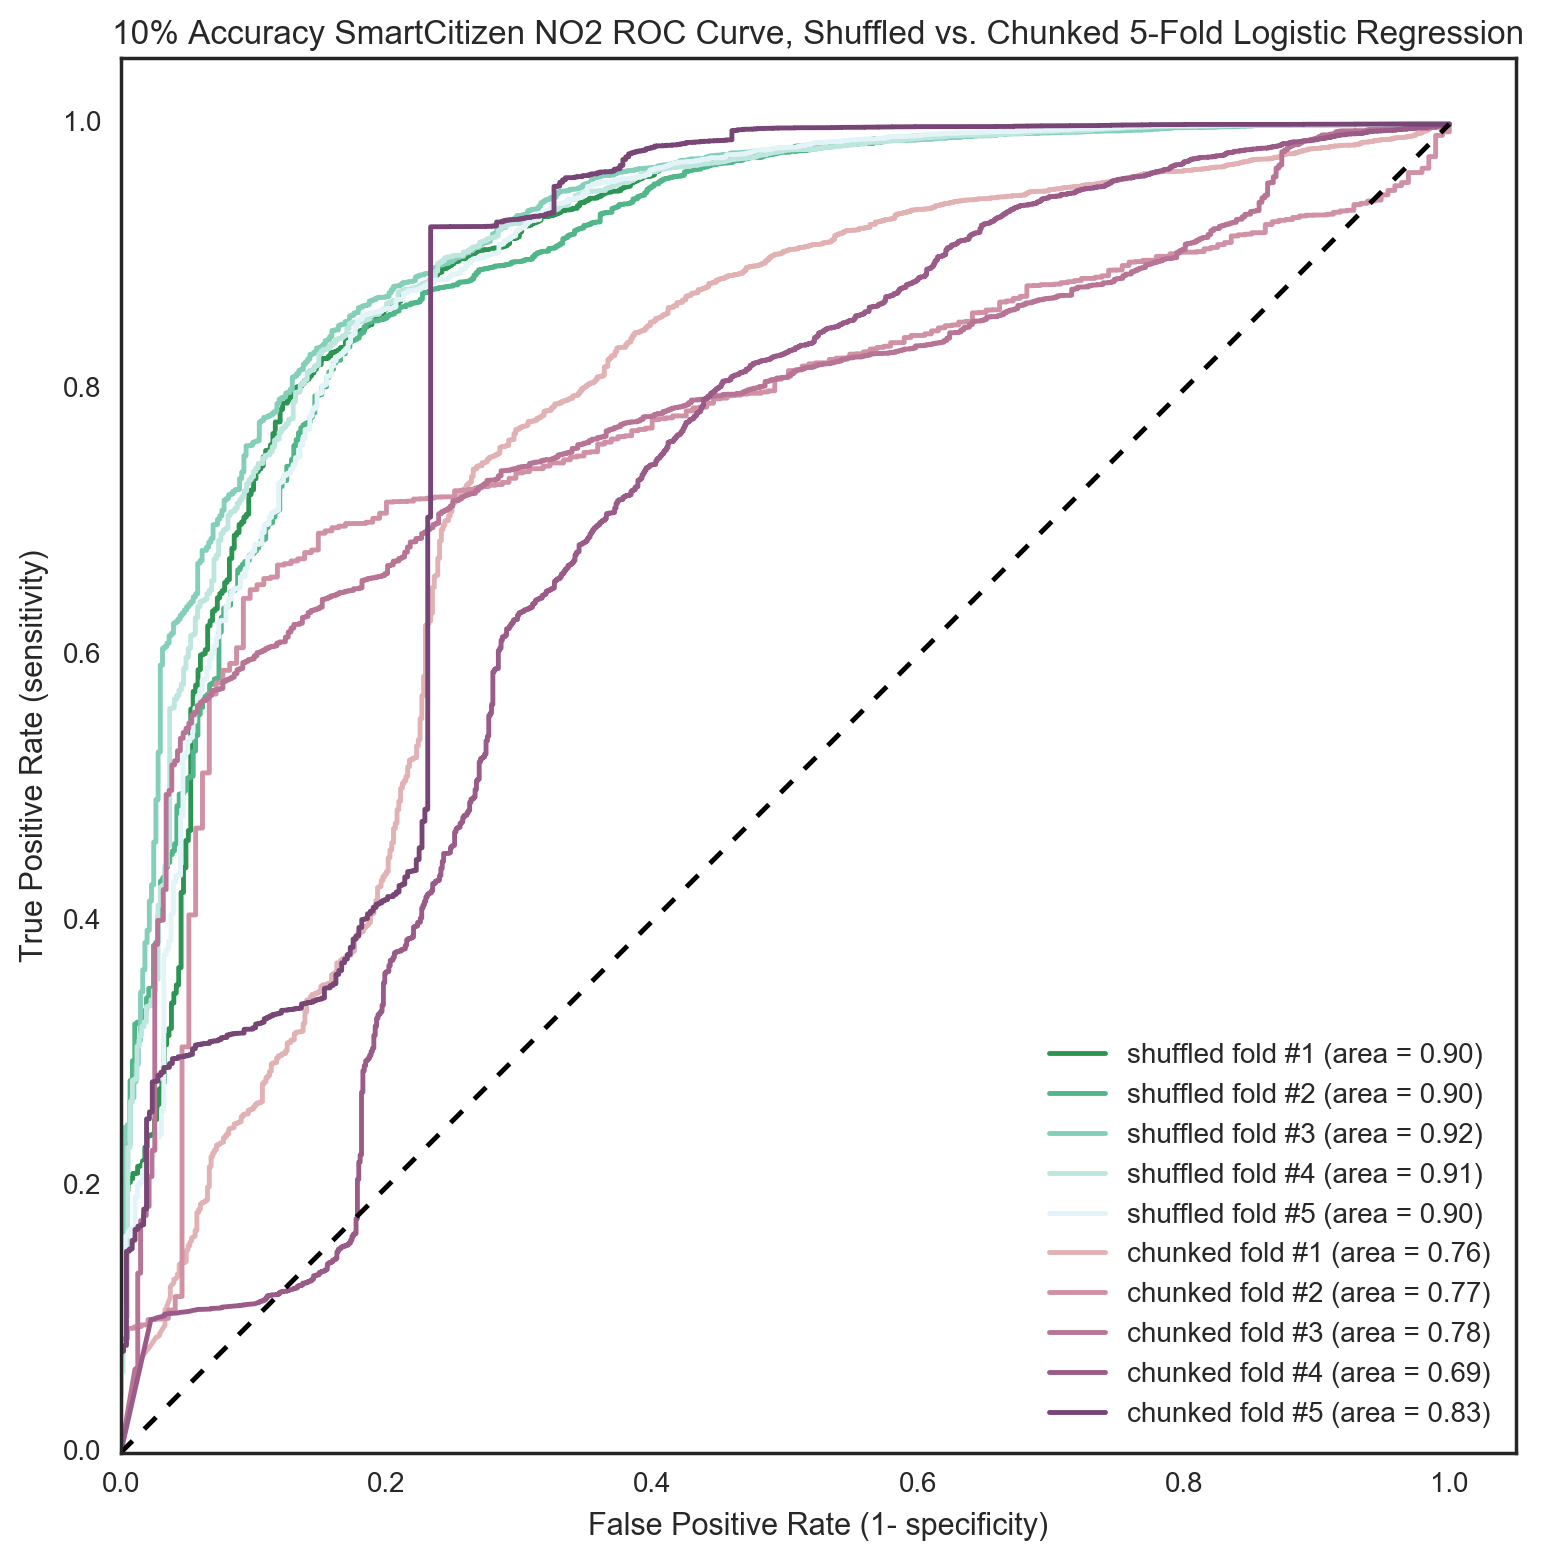
\includegraphics[width=\textwidth]{figs/sck_no2_10_roc}               
 	 \caption{SmartCitizen NO2 ROC Curve}
  	\label{fig:sck_no2_10_roc}
\end{figure}


We see similar error rates with all features as for a subset of the top fifteen.  Examining the AUC-ROC shows that when training only with the top features, the score drops from 0.9 to 0.8 -- a substantial drop, but proof that the top fifteen account for a very strong prediction on their own.


\begin{table}[htb]
\centering
\small
\begin{tabular}{lllllllll}
\\
\\
\toprule
     & Corr. & Lasso & Lin Reg & RF   & RFE  & Ridge & Stability & Mean \\
\midrule
bkcarbon                                   & 1     & 0          & 0    & 1    & 0.63  & 0.51      & 0.85 & 0.57 \\
daily\_avg\_sck\_humidity                  & 0.11  & 0          & 0    & 0.32 & 0.67  & 1         & 0.76 & 0.41 \\
hour\_of\_day                              & 0.07  & 0.92       & 0    & 0.1  & 0.42  & 0.02      & 1    & 0.36 \\
avg\_60\_bkcarbon                          & 0.92  & 0          & 0    & 0.08 & 0.59  & 0.25      & 0.69 & 0.36 \\
derivative\_avg\_1440\_lmse\_calib\_as\_co & 0.06  & 0          & 0    & 0.05 & 0.62  & 0.38      & 1    & 0.3  \\
Solar Panel ( V)                           & 0.03  & 0          & 1    & 0    & 0.88  & 0         & 0    & 0.27 \\
lmse\_sck\_co                              & 0.01  & 1          & 0    & 0.02 & 0.85  & 0         & 0    & 0.27 \\
derivative\_avg\_1440\_bkcarbon            & 0.05  & 0          & 0    & 0.07 & 0.71  & 0.1       & 0.99 & 0.27 \\
humidity\_box\_differential                & 0.02  & 0          & 0.04 & 0.11 & 1     & 0.61      & 0    & 0.25 \\
forecastio\_partly-cloudy-night            & 0.03  & 0          & 0.16 & 0.02 & 0.95  & 0.11      & 0.42 & 0.24 \\
avg\_60\_forecastio\_humidity              & 0     & 0          & 0.04 & 0.06 & 1     & 0.61      & 0    & 0.24 \\
day                                        & 0.07  & 0          & 0    & 0    & 0.97  & 0.05      & 0.51 & 0.23 \\
night                                      & 0.07  & 0          & 0.01 & 0    & 0.98  & 0.05      & 0.43 & 0.22 \\
avg\_60\_forecastio\_precipProbability     & 0.04  & 0          & 0    & 0    & 0.6   & 0.49      & 0.44 & 0.22 \\
daily\_avg\_forecastio\_humidity           & 0.03  & 0          & 0    & 0.05 & 0.66  & 0.48      & 0.24 & 0.21 \\
forecastio\_rain                           & 0.03  & 0          & 0.16 & 0    & 0.9   & 0.25      & 0.04 & 0.2  \\
forecastio\_humidity                       & 0     & 0          & 0    & 0    & 0.64  & 0.72      & 0    & 0.19 \\
forecastio\_clear-night                    & 0.02  & 0          & 0.16 & 0    & 0.93  & 0.03      & 0.1  & 0.18 \\
forecastio\_fog                            & 0     & 0          & 0.16 & 0    & 0.9   & 0.21      & 0    & 0.18 \\
forecastio\_wind                           & 0.01  & 0          & 0.16 & 0    & 0.92  & 0.18      & 0    & 0.18 \\
avg\_720\_bkcarbon                         & 0.47  & 0          & 0    & 0.05 & 0.54  & 0.07      & 0.12 & 0.18 \\
avg\_30\_ws                                & 0.13  & 0          & 0    & 0.08 & 0.45  & 0.02      & 0.48 & 0.17 \\
avg\_15\_derivative\_sck\_temperature      & 0     & 0          & 0    & 0.04 & 0.63  & 0.5       & 0.01 & 0.17 \\
avg\_720\_lmse\_scaled\_sharpDust          & 0.01  & 0          & 0    & 0.16 & 0.58  & 0.41      & 0    & 0.17 \\
\bottomrule
\end{tabular}
\label{tab:sck_no2_top_features}
\caption{Top Features for Predicting SmartCitizen NO2}
\end{table}

 
The top features are similar to those that predicted the CO transients, but with a stronger relationship-- black carbon is a leading indicator, as well as humidity, the hour of the day, and CO level.  These all make sense as correlates-- CO and black carbon are produced by traffic, which has a predictable pattern with the time of day.  Table \ref{tab:sck_no2_top_features}) shows the top features given seven feature selection algorithms.

\begin{margintable}
\centering
\offinterlineskip
\hspace*{-5cm}\raisebox{-4cm}[0pt][0pt]{\rotatebox[origin=c]{90}{\parbox[c][0pt][c]{3cm}{\textbf{Actual Values}\\[20pt]}}}\par
\hspace{.3cm}\MyHBox[\marginparwidth]{Predicted Values}\par
\vspace{-.5cm}
\hspace*{1cm}\MyHBox{0}\MyHBox{1}\par
\MyTBox{0}{142.0}{427.0}
\vspace{-.35cm}\MyTBox{1}{52.6}{14370.2}\raisebox{-1cm}
}
\label{tab:sck_no2_confusion}
\caption{Average SmartCitizen NO2 Confusion Matrix w/Shuffled K-Fold}
\end{margintable}

Once again, there seems to be strong evidence that NO2 transients are highly predictable if there are other, good quality sensors that measure related phenomena (like black carbon and CO) to rely on.  The relationship is a complex one that requires a larger feature set and a lot of training data for optimal performance, but it appears that even in the short two month period we were able to train a model that would work well under realistic conditions.


\FloatBarrier

\section{Sharp Dust Sensor}
This is about the Sharp Particulate Sensor results.

One Sharp optical particulate sensor was tested against the EPA black carbon reference.  It was 1 month old at the time of installation, and ran for 59 days (from 4/15 - 6/13 2016) with two ~40 minute service interruptions.  This test gave 1,431 samples of hour resolution data.


\subsection{Pre-processing}

Talk about process for taking raw aux/working electrodes and making the basic calibration data.
10am reading of EPA sensor is recorded on filter paper from 10a-10:50a, then measured with Beta Attenuation from 10:50-11a.  Thus, we averaged the 50 minute readings starting on the hour and threw away the last ten minutes.  Added some feature averaging on the 6hr , 12hr, day scale.

\begin{figure}[htb]
 	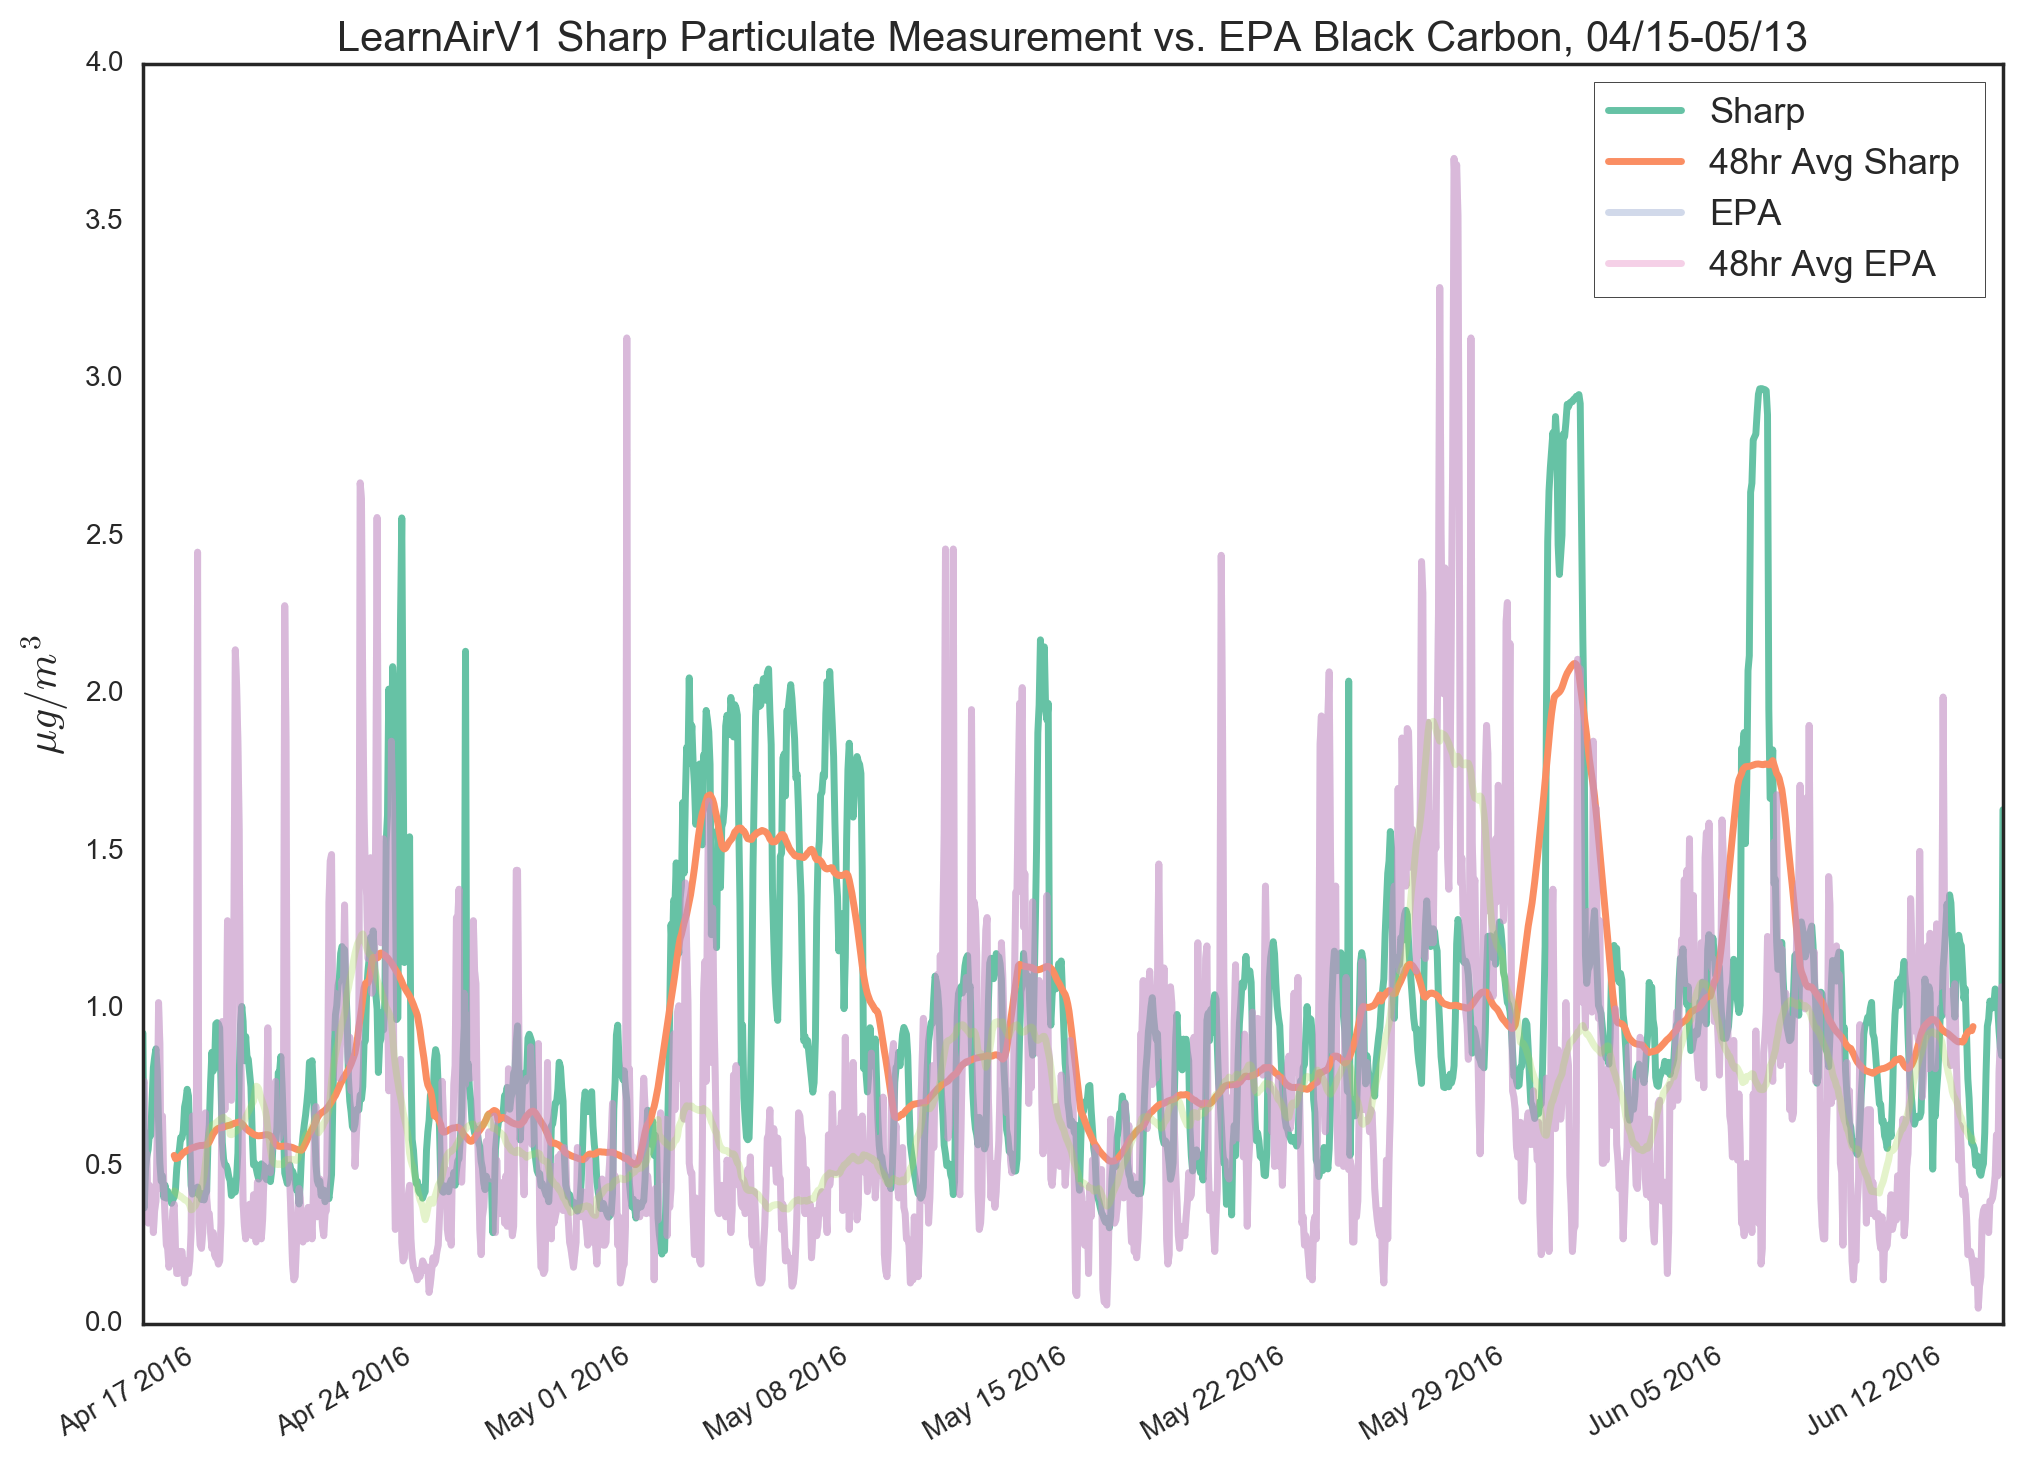
\includegraphics[width=\textwidth]{figs/sharp_raw}               
 	 \caption{Sharp Raw Particulate Data}
  	\label{fig:sharp_raw}
\end{figure}


\begin{figure}[htb]
 	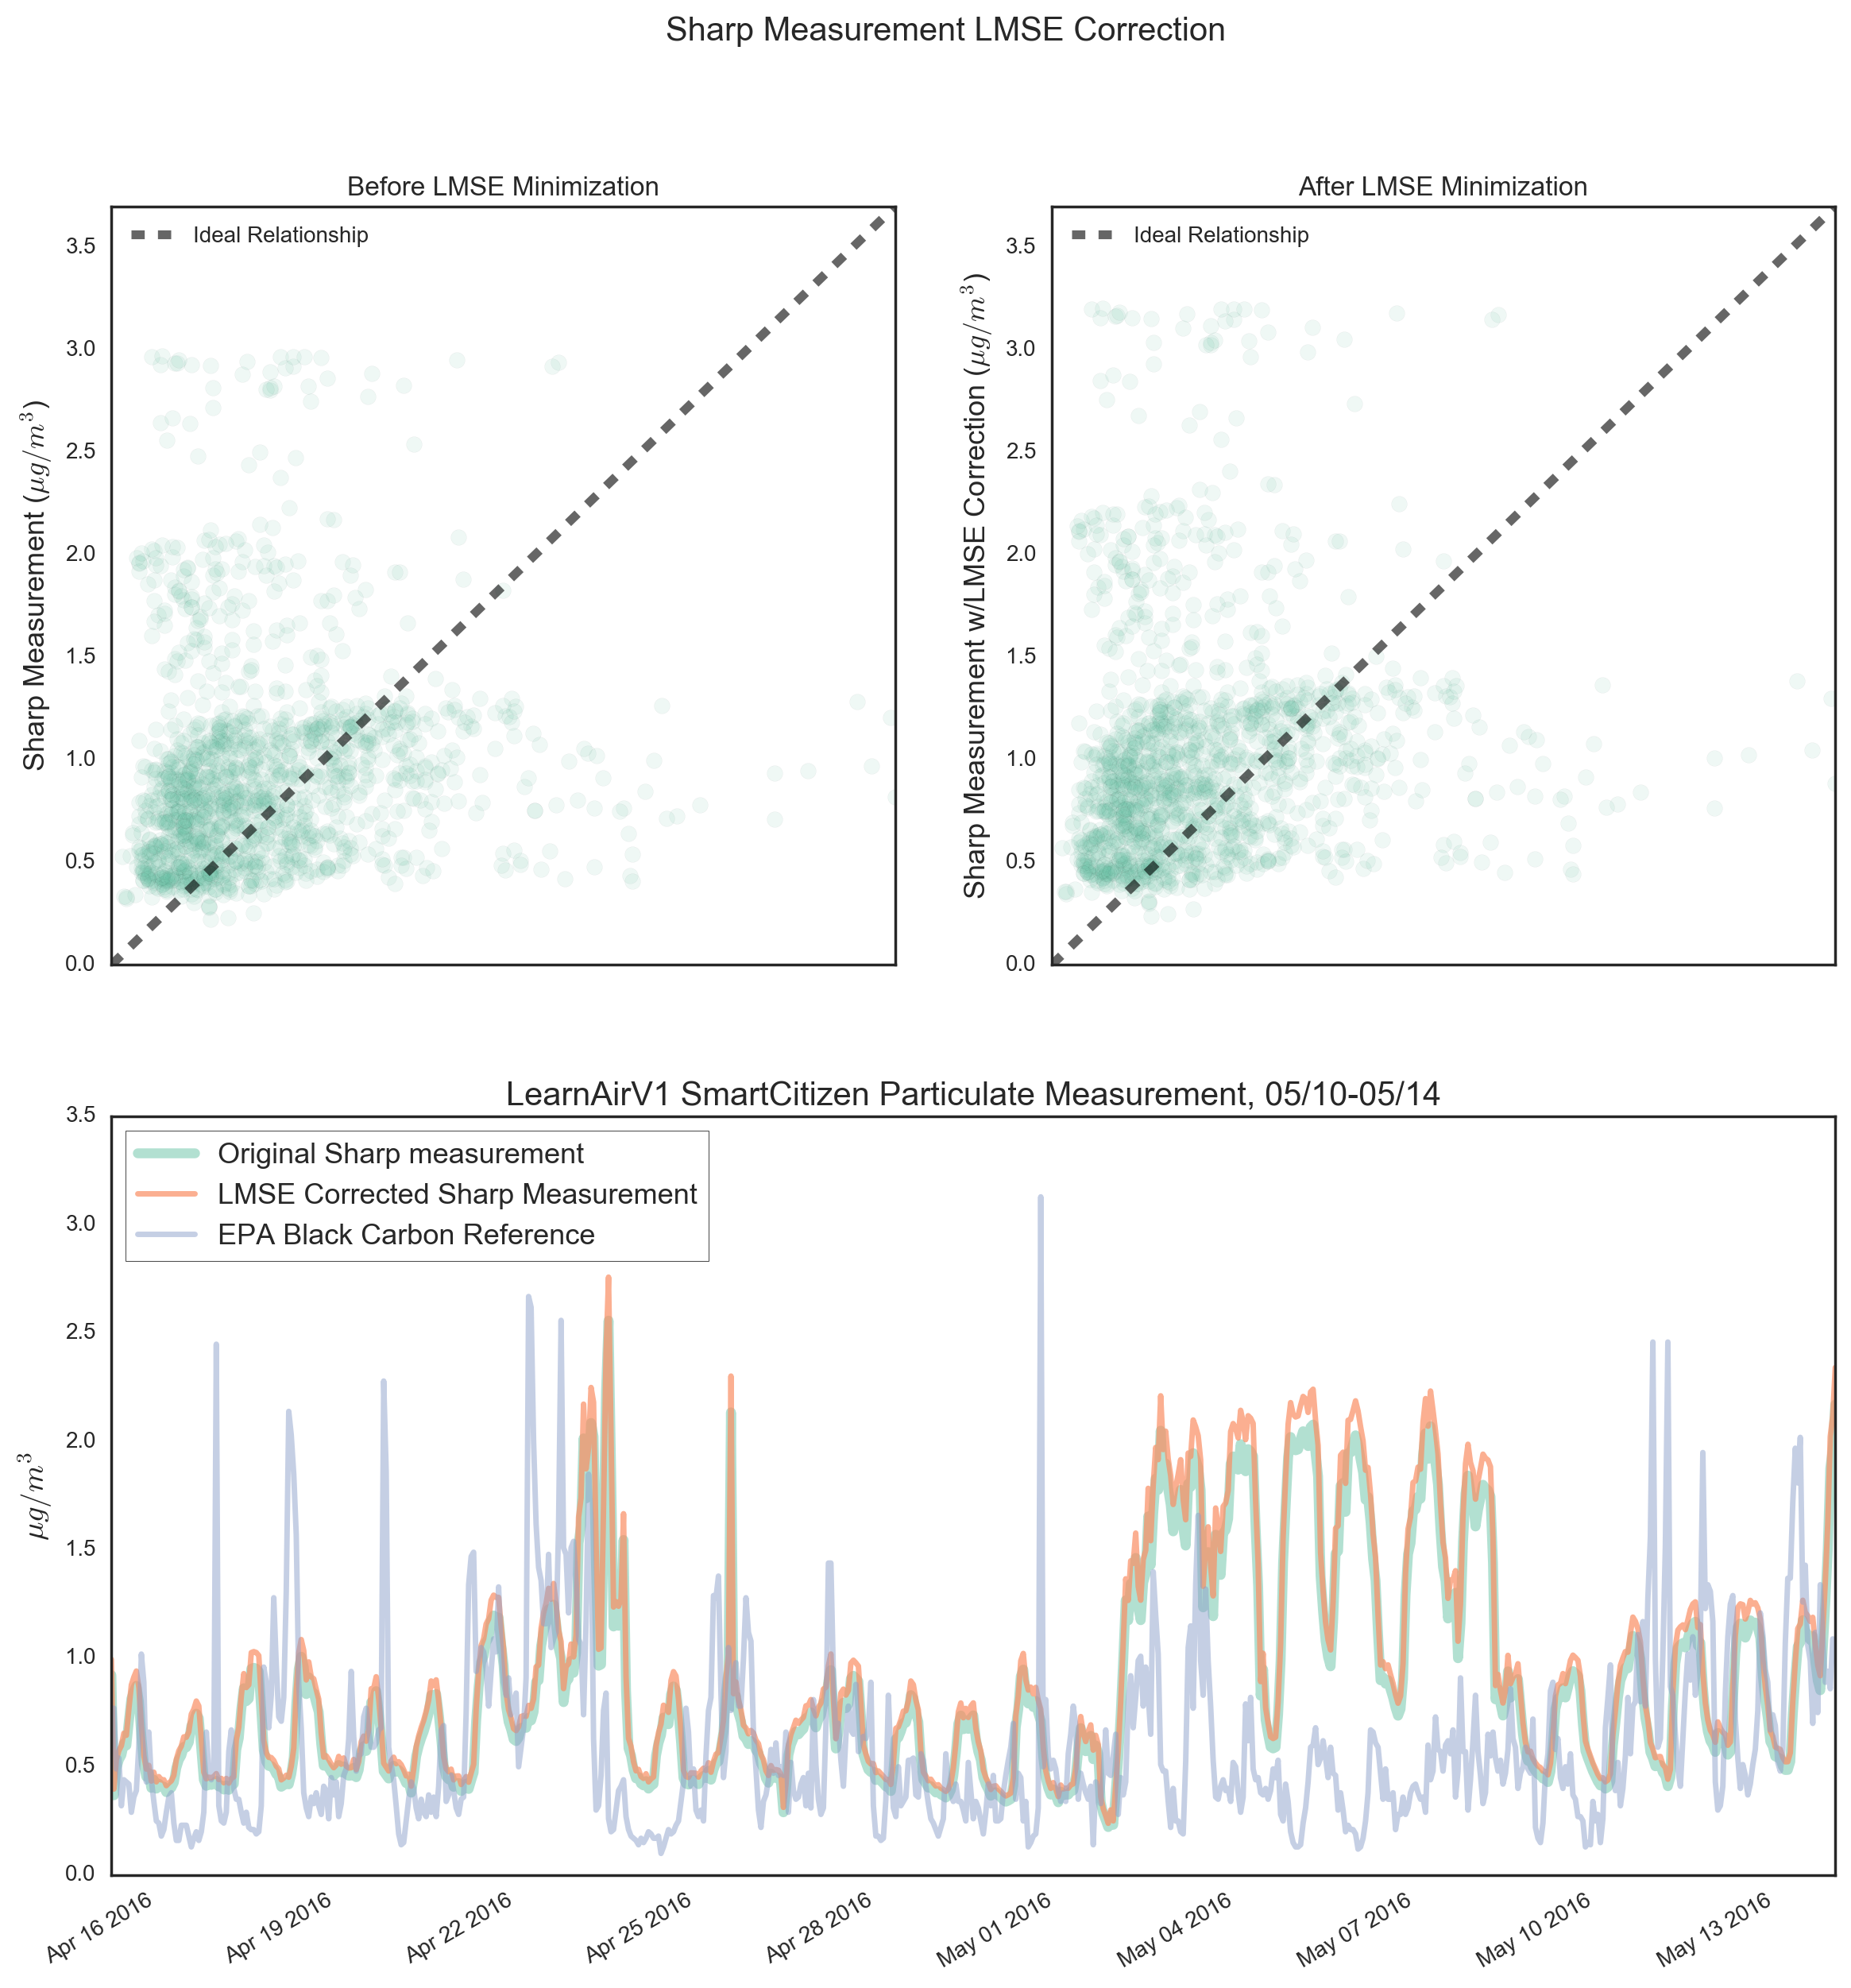
\includegraphics[width=\textwidth]{figs/sharpDust_lmse}               
 	 \caption{Sharp Particulate LMSE Calibration}
  	\label{fig:sharpDust_lmse}
\end{figure}

\begin{figure}[htb]
 	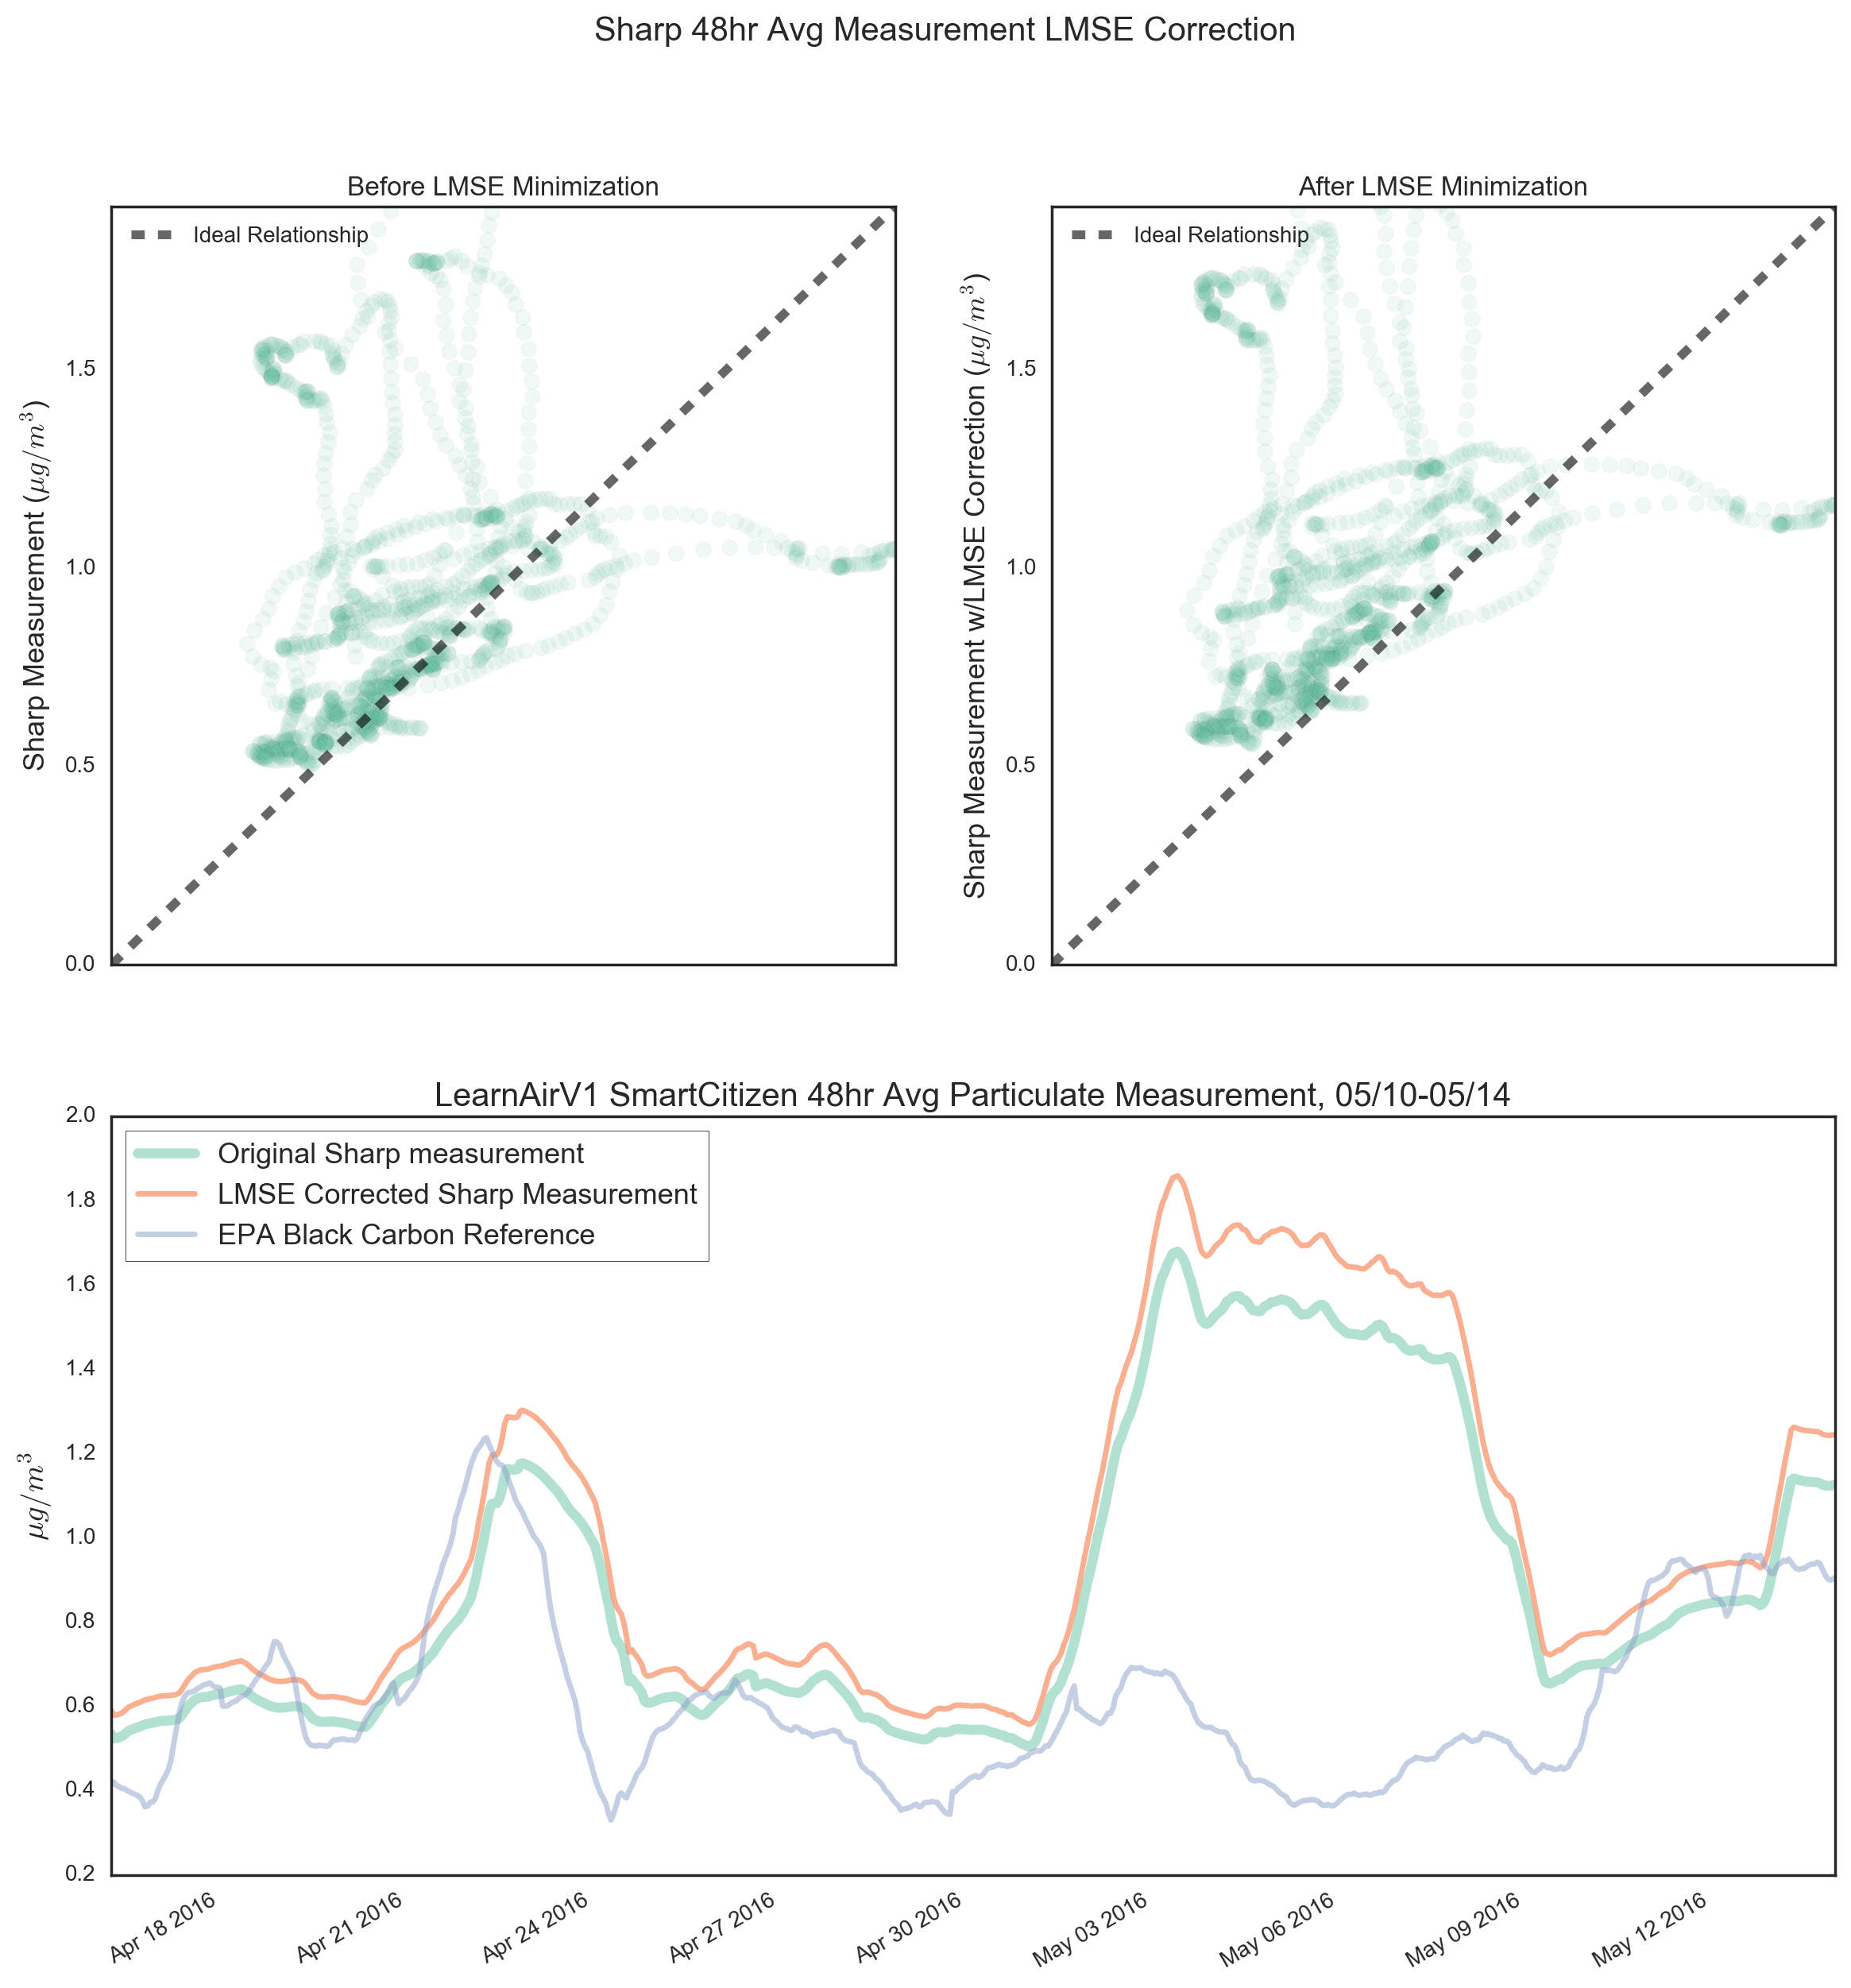
\includegraphics[width=\textwidth]{figs/sharpDust_avg_48_lmse}               
 	 \caption{2 day Average Sharp Particulate LMSE Calibration}
  	\label{fig:sharpDust_avg_48_lmse}
\end{figure}







\subsection{Machine Learning}


\begin{figure}[htb]
 	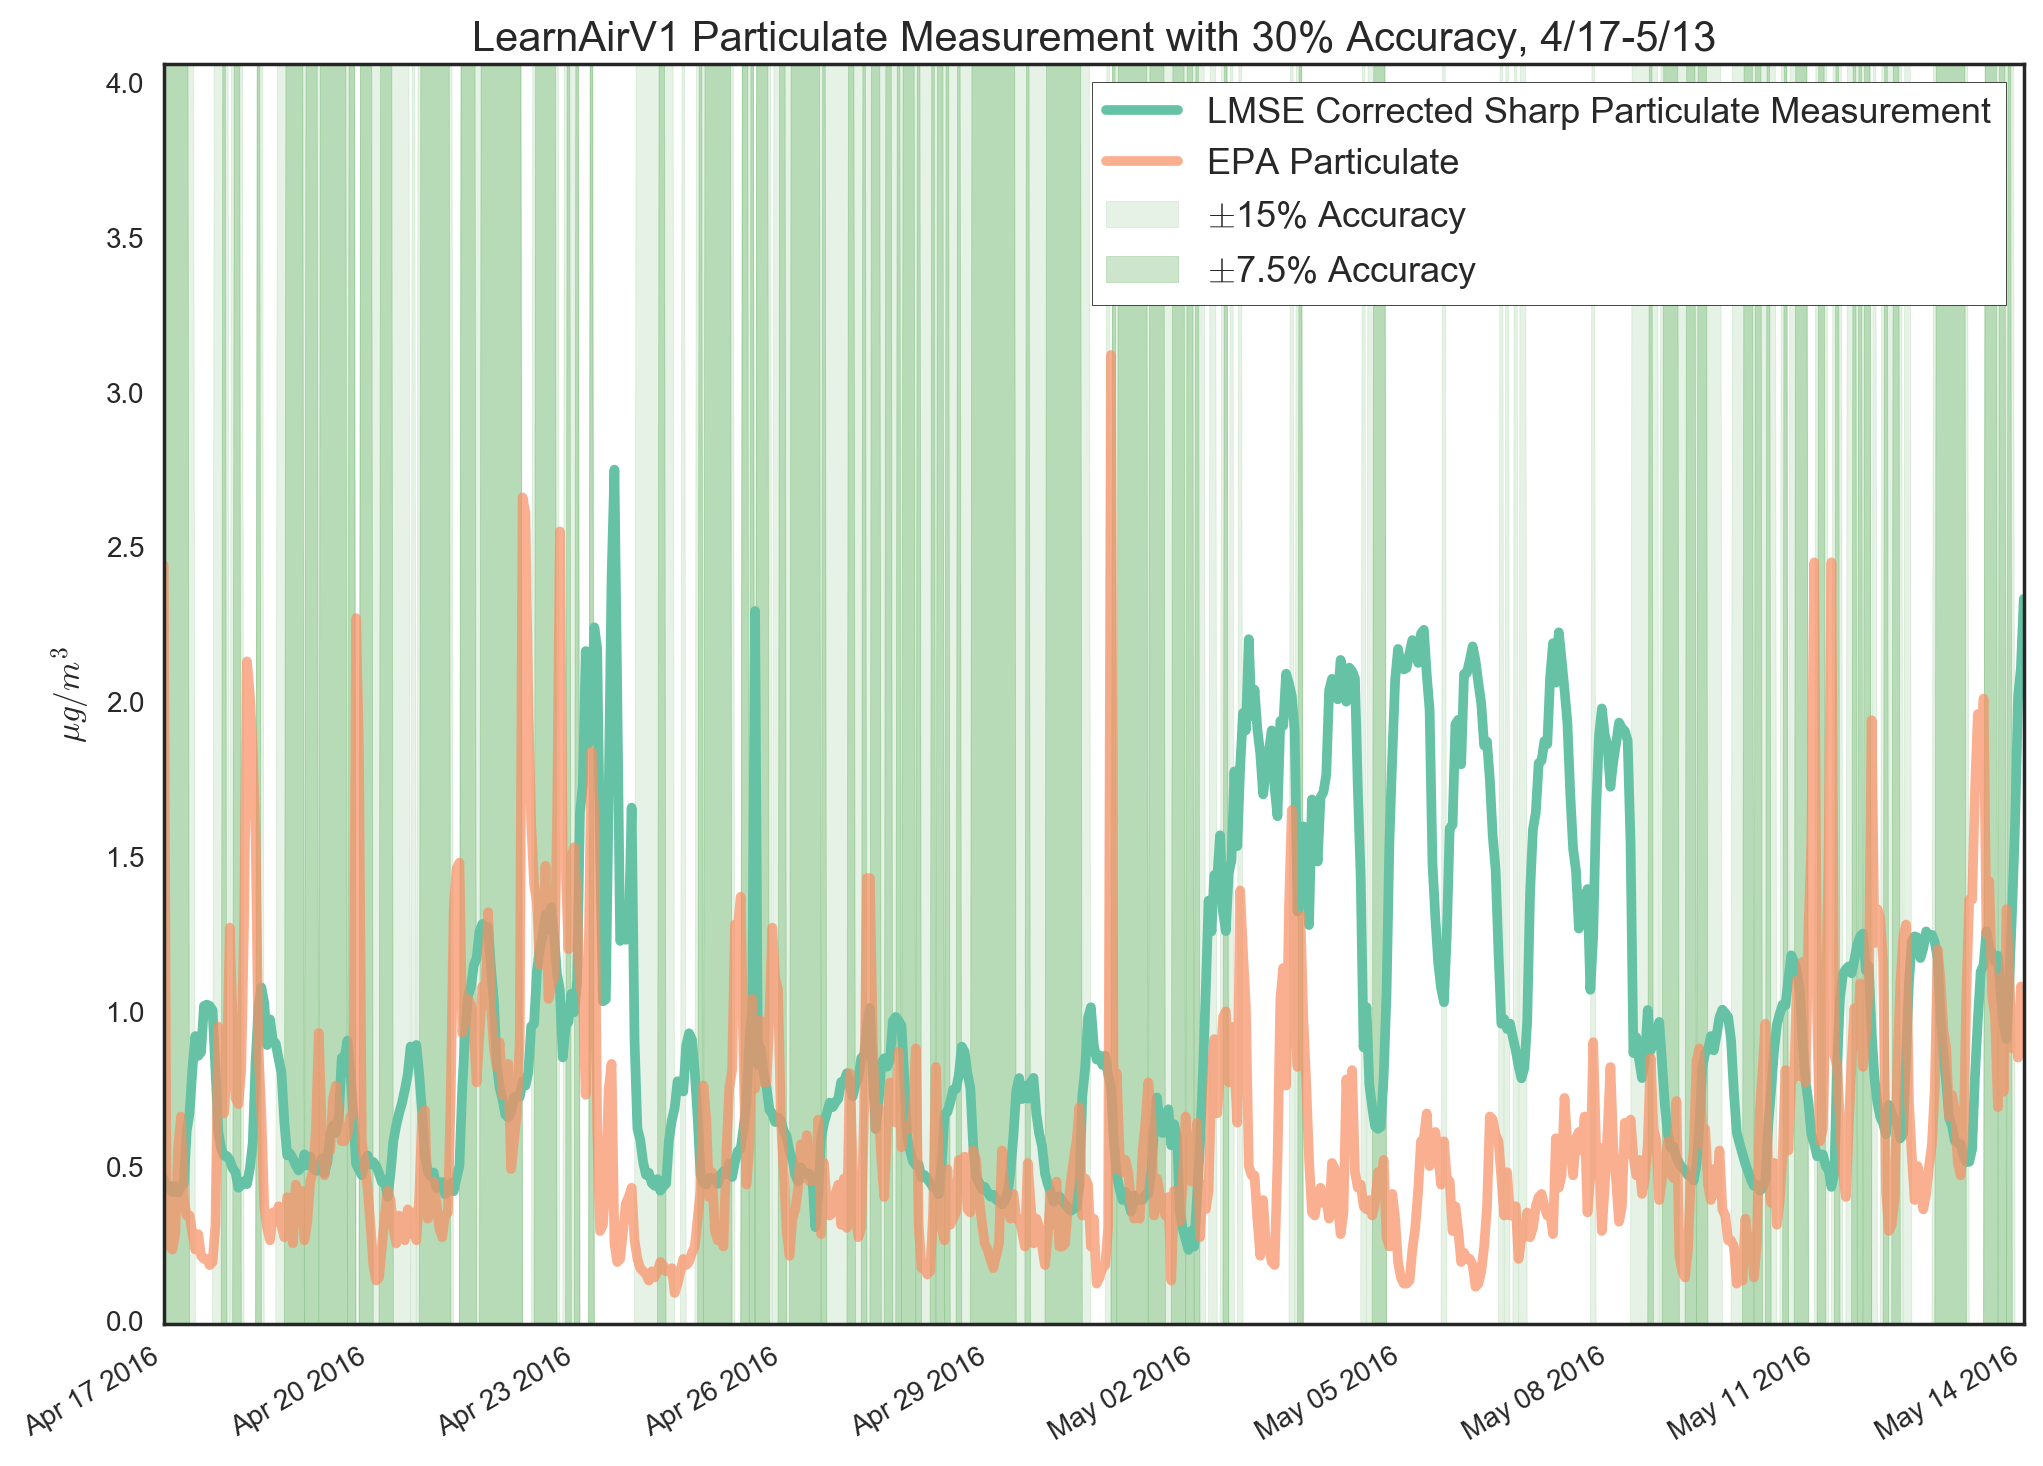
\includegraphics[width=\textwidth]{figs/sharpDust_with_accuracy_zoomed}               
 	 \caption{Sharp Particulate with 30\% Accuracy Threshold}
  	\label{fig:sharpDust_with_accuracy_zoomed}
\end{figure}




parameters = {'C':[0.001, 0.01, 0.1, 1, 10, 100, 1000], 'penalty':('L1', 'L2') }, true 5 fold validation

===== best ROC\_AUC score 0.868191734814

===== best params {'penalty': 'L1', 'C': 1}



\begin{table}[H]
\centering
\begin{tabular}{|c|c|c|c|c|}
\toprule
\multicolumn{5}{|c|}{Error Rates for CO Sensor #1 with Logistic Regression} \\
&\multicolumn{2}{|c|}{all features} & \multicolumn{2}{|c|}{top 15 features} \\
&shuffled & chunked & shuffled & chunked \\
avg & 0.17 & 0.22 & 0.22 & 0.25 \\
min & 0.14 & 0.18 & 0.20 & 0.14 \\
max & 0.20 & 0.29 & 0.24 & 0.36 \\
\bottomrule
\end{tabular}
\label{tab:as1_co_error_rates}
\caption{Error Rates for Predicting Sharp Accuracy with Logistic Regression}
\end{table}



\begin{table}[H]
\centering
\offinterlineskip
\hspace*{-5cm}\raisebox{-3.5cm}[0pt][0pt]{\rotatebox[origin=c]{90}{\parbox[c][0pt][c]{3cm}{\textbf{Actual Values}\\[20pt]}}}\par
\hspace*{1cm}\MyHBox[\dimexpr5.1cm+6\fboxsep\relax]{Predicted Values}\par
\hspace*{1cm}\MyHBox{0}\MyHBox{1}\par
\MyTBox{0}{58.0}{35.2}
\MyTBox{1}{14.0}{179.0}
}
\label{tab:as1_co_confusion}
\caption{Average Sharp Particulate Confusion Matrix w/Shuffled K-Fold}
\end{table}


\begin{figure}[htb]
 	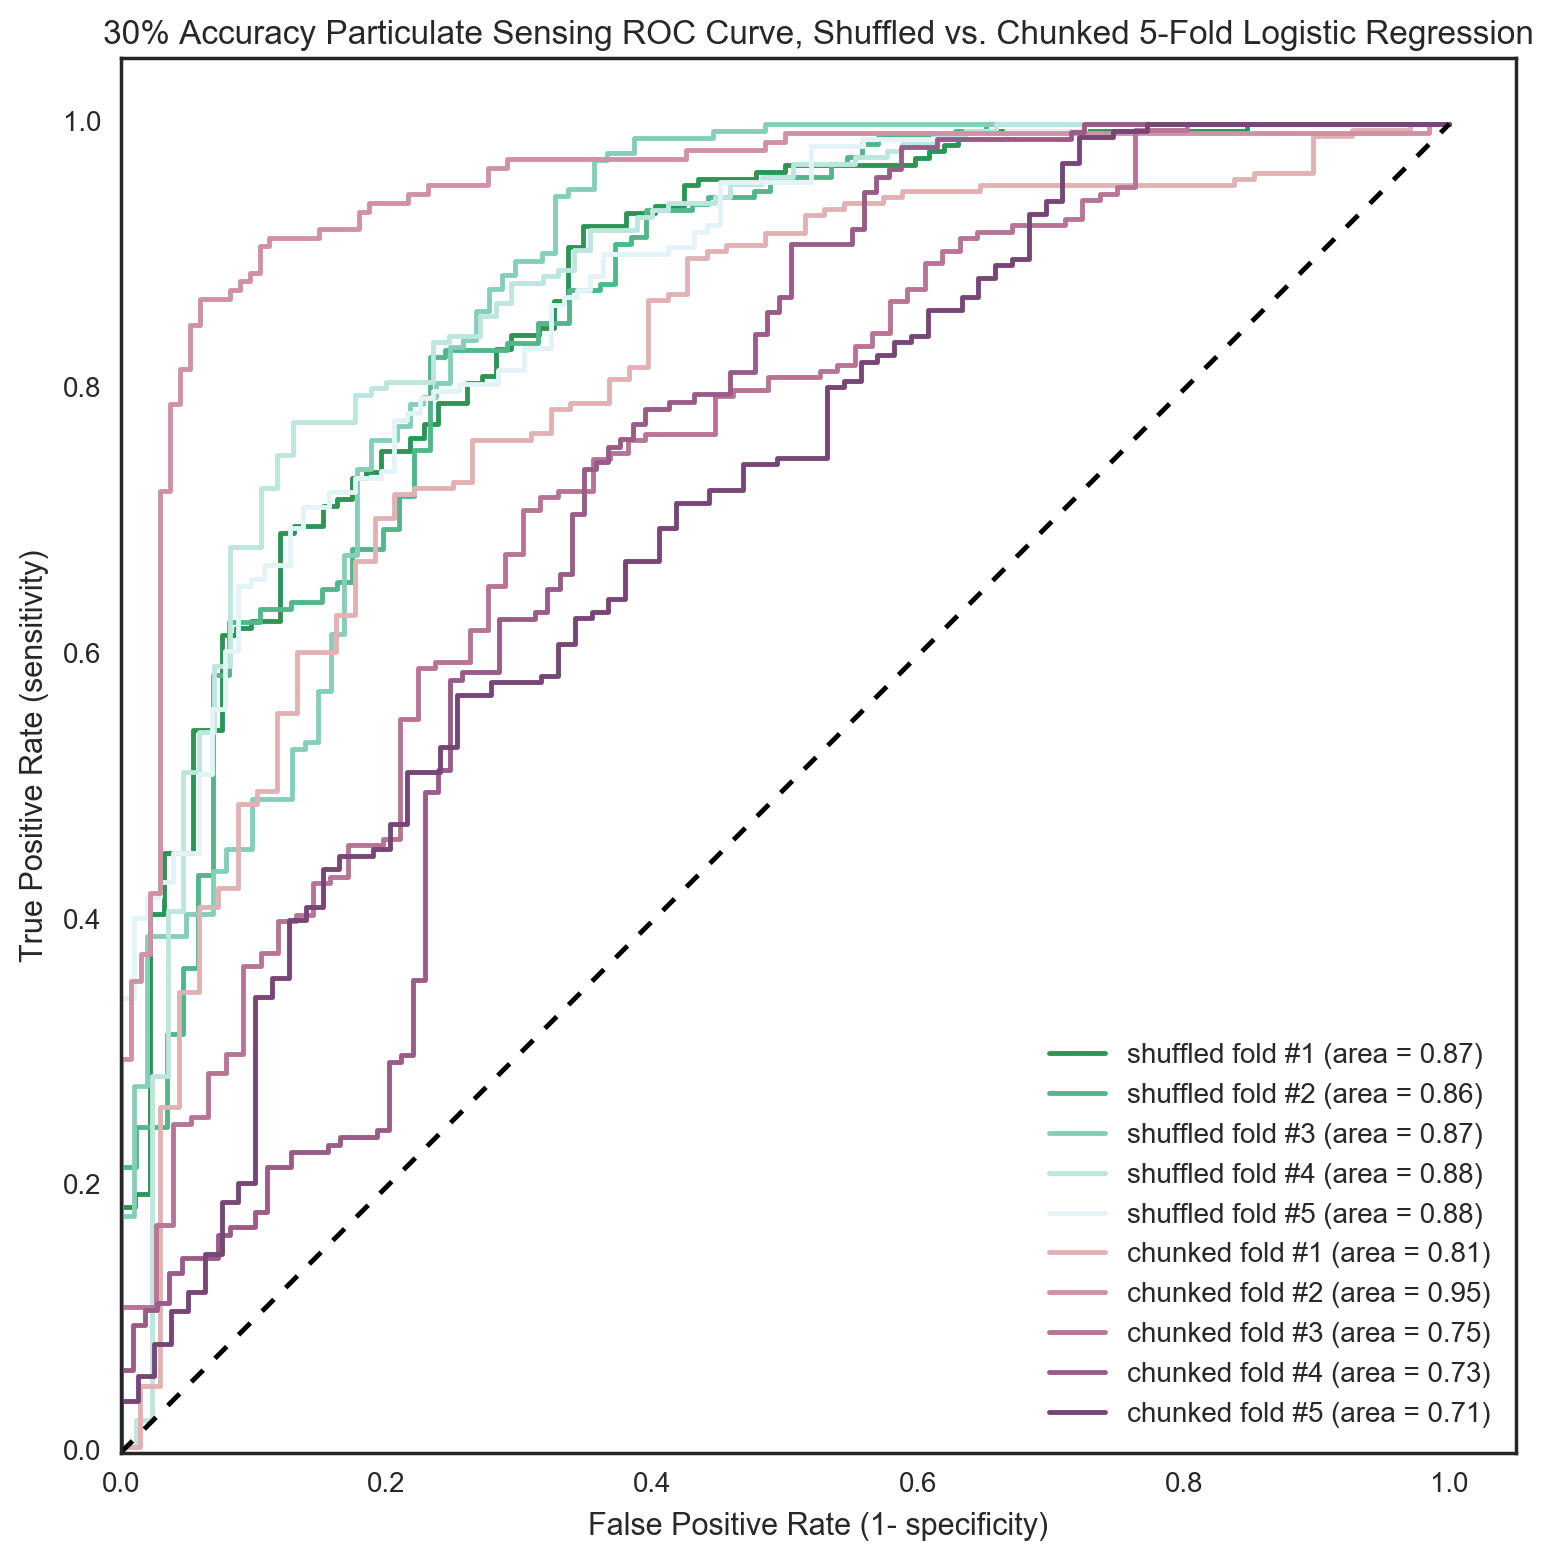
\includegraphics[width=\textwidth]{figs/sharp_goals_30_roc}               
 	 \caption{Sharp Particulate ROC Curve}
  	\label{fig:sharp_30_roc}
\end{figure}


here's text referencing the (Table \ref{tab:sharp_randomforest_features}).

\begin{table}[H]
\centering
\begin{tabular}{lllllllll}
\\
\\
\toprule
Feature & Importance \\
\midrule
 scaled\_sharpDust &  0.039935725943 \\
 avg\_12\_scaled\_sharpDust &  0.0390147943972 \\
 sharpDust &  0.0390147211728 \\
 lmse\_scaled\_sharpDust &  0.0381632767126 \\
 avg\_48\_scaled\_sharpDust &  0.0225005941711 \\
 lmse\_avg\_48\_scaled_sharpDust &  0.0207695248823 \\
 sck\_humidity &  0.0163292725576 \\
 Humidity ( % RAW) &  0.0162400825573 \\
 no2 &  0.0149758603207 \\
 daily\_avg\_sck\_humidity &  0.0138699992039 \\
 daily\_avg\_forecastio\_humidity &  0.0132135840929 \\
 humidity\_box\_differential &  0.0119641893085 \\
 co &  0.0118968560369 \\
 sck\_humidity\_saturated &  0.0103888721788 \\
 avg\_60\_forecastio\_humidity &  0.0102980544091 \\
\bottomrule
\end{tabular}
\label{tab:sharp_randomforest_features}
\caption{Top 15 Features from Random Forest for Sharp Sensor, used in Pruned Logistic Regression}
\end{table}



\begin{figure}[htb]
 	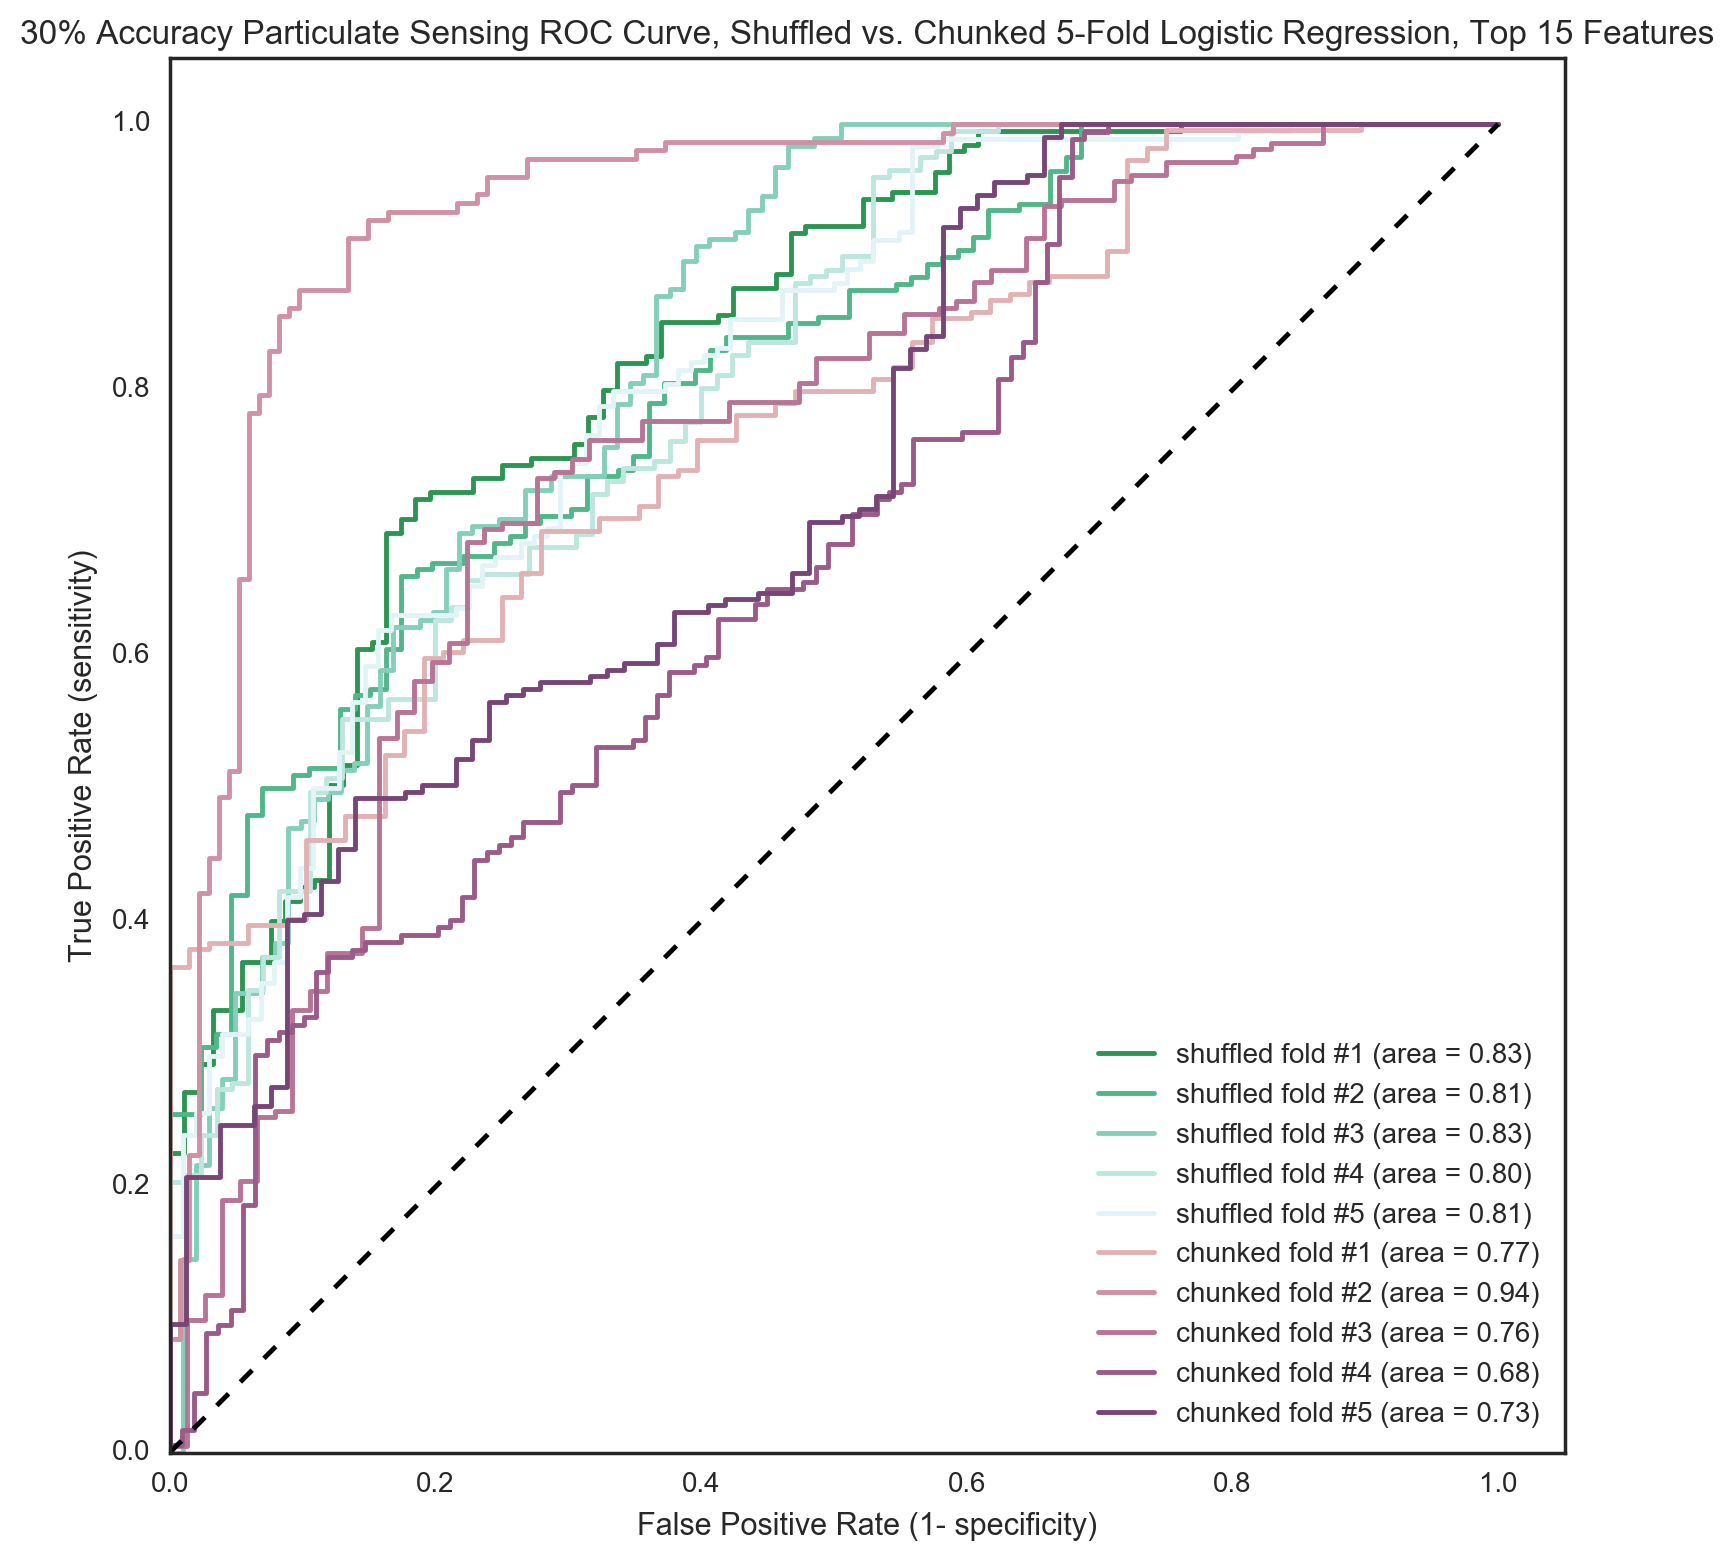
\includegraphics[width=\textwidth]{figs/sharp_goals_30_roc_pruned_features}               
 	 \caption{Sharp Particulate ROC Using Top 15 Features}
  	\label{fig:sharp_30_roc_pruned_features}
\end{figure}

\begin{figure}[htb]
 	\includegraphics[width=\textwidth]{figs/sharp_goals_30_logistic_predictions}               
 	 \caption{Sharp Particulate Prediction Accuracy}
  	\label{fig:sharp_30_logistic_predictions}
\end{figure}



here's text referencing the (Table \ref{tab:sharp_top_features}).

\begin{table}[H]
\centering
\begin{tabular}{lllllllll}
\\
\\
\toprule
     & Corr. & Lasso & Lin Reg & RF   & RFE  & Ridge & Stability & Mean \\
\midrule
sharpDust                                    & 1     & 0.65       & 0    & 1    & 0.81  & 0.03      & 1    & 0.64 \\
lmse\_scaled\_sharpDust                      & 1     & 0          & 0.03 & 0.65 & 0.83  & 0         & 0.98 & 0.5  \\
scaled\_sharpDust                            & 1     & 0          & 0.02 & 0.65 & 0.83  & 0         & 0.91 & 0.49 \\
avg\_12\_scaled\_sharpDust                   & 0.88  & 0          & 0    & 0.06 & 0.49  & 0.77      & 0.55 & 0.39 \\
derivative\_lmse\_avg\_15\_as\_no2           & 0     & 0          & 0.99 & 0    & 0.97  & 0.15      & 0.02 & 0.3  \\
derivative\_avg\_15\_lmse\_as\_no2           & 0     & 0          & 1    & 0    & 0.97  & 0.15      & 0.01 & 0.3  \\
derivative\_avg\_48\_scaled\_sharpDust       & 0.01  & 0          & 0.99 & 0.01 & 1     & 0.01      & 0    & 0.29 \\
derivative\_lmse\_avg\_48\_scaled\_sharpDust & 0.01  & 0          & 0.89 & 0.03 & 1     & 0.01      & 0    & 0.28 \\
temp\_as\_box\_differential                  & 0.01  & 1          & 0    & 0.22 & 0.47  & 0.13      & 0.05 & 0.27 \\
sck\_humidity\_saturated                     & 0.11  & 0          & 0    & 0    & 0.61  & 1         & 0.01 & 0.25 \\
Nitrogen Dioxide ( kOhm)                     & 0.18  & 0.06       & 0    & 0.02 & 0.72  & 0         & 0.67 & 0.24 \\
daily\_avg\_sck\_humidity                    & 0.24  & 0          & 0    & 0.05 & 0.6   & 0.69      & 0    & 0.23 \\
lmse\_sck\_no2                               & 0.18  & 0          & 0    & 0.02 & 0.72  & 0         & 0.67 & 0.23 \\
avg\_48\_scaled\_sharpDust                   & 0.45  & 0          & 0.02 & 0.01 & 0.88  & 0.18      & 0.07 & 0.23 \\
lmse\_avg\_48\_scaled\_sharpDust             & 0.45  & 0          & 0.02 & 0.01 & 0.87  & 0.2       & 0.06 & 0.23 \\
forecastio\_wind                             & 0     & 0          & 0    & 0    & 0.96  & 0.58      & 0    & 0.22 \\
derivative\_as\_no2                          & 0     & 0          & 0    & 0    & 0.99  & 0.57      & 0    & 0.22 \\
o3                                           & 0.1   & 0.25       & 0    & 0.06 & 0.14  & 0.01      & 0.85 & 0.2  \\
derivative\_Carbon Monxide ( kOhm)           & 0     & 0          & 0.36 & 0.03 & 0.99  & 0.01      & 0    & 0.2  \\
derivative\_lmse\_sck\_no2                   & 0     & 0          & 0.45 & 0.01 & 0.86  & 0         & 0    & 0.19 \\
derivative\_lmse\_sck\_co                    & 0     & 0          & 0.31 & 0.02 & 0.98  & 0.01      & 0    & 0.19 \\
daily\_avg\_forecastio\_humidity             & 0.29  & 0          & 0    & 0.02 & 0.46  & 0.41      & 0.05 & 0.18 \\
forecastio\_rain                             & 0.08  & 0          & 0    & 0    & 0.92  & 0.18      & 0    & 0.17 \\
alphaTemp                                    & 0     & 0          & 0    & 0.01 & 0.75  & 0.39      & 0    & 0.16 \\
\bottomrule
\end{tabular}
\label{tab:sharp_top_features}
\caption{Top Features for Predicting Sharp Particulate}
\end{table}

End Text for Sharp Section.

\FloatBarrier

\section{AlphaSense CO}
Two AlphaSense CO sensors were tested against the EPA reference.  The first sensor was 2.5 years old at the time of installation,  which ran for 38 days (from 4/15 to 5/23 2016 with one 40 minute service interruption).  The second sensor was 2 months old at the time of installation, and ran for 21 days (from 5/23 - 6/13 2016).  Our first test gave 55,589 minute-resolution samples to compare, our second test gave 30,150 samples.

These two tests give us a chance to compare manufacturer reliability and sensor aging effects.  The two datasets can also be combined after calibration to draw overall conclusions about the AlphaSense model CO-A4 sensor.  

\subsection{Pre-processing}

AlphaSense sensors give two main readings-- from an auxilary and a working electrode.  Additionally, they come with a calibration for sensitivity, as well as offset voltages for both electrodes.  The calibration function combines all of these using a non-linear temperature-dependent term.  

While we used the provided calibration data to create one version of `corrected data', we've found from talking with faculty in the Evironmental Engineering group that it is not uncommon for these laboratory based calibrations to be poor quality.  It is generally best practice to calibrate the sensors using co-location data.  The provided calibration provides results as seen in Figure \ref{fig:as_co_raw_zoomed}.

\begin{figure}[htb]
 	\includegraphics[width=\textwidth]{figs/as_co_raw_zoomed}               
 	 \caption{AlphaSense CO Sensor #1 Raw Data Zoomed}
  	\label{fig:as_co_raw_zoomed}
\end{figure}

We tried three LMSE minimzation techniques for better calibration after applying the datasheet calibration information-- once again we simply scale/offset the data, we scale/offset using only the data within one standard deviation of the mean (in order to remove outliers), and finally we solve for optimal sensitivity and offset voltages using the actual calibration equation and seeding it with the AlphaSense supplied values.  The third method-- solving for new calibration terms in the provided (non-linear, temperature dependent) calibration equation-- gave the best results by a significant margin.  The results of this technique for both the older and newer sensors can be seen in Figures \ref{fig:as2_co_lmse} and \ref{fig:as_co_with_5_accuracy_zoomed}.

\begin{figure}[htb]
 	\includegraphics[width=\textwidth]{figs/as2_co_lmse}               
 	 \caption{AlphaSense CO Sensor #2 after LMSE Calibration}
  	\label{fig:as2_co_lmse}
\end{figure}

\subsection{Machine Learning}

These sensors have some 

5V / (2^10) = 4.88 mV resolution on the ADC.  Sensor speced for ~0.3 mV/ppb. We expect a quantization to limit our resolution to ~16 ppb steps.  The AFE is speced for a noise level of ~20 ppb.  


Both sensors were treated independently to start, and their output was compared.  Agreement between the two can provide us with high confidence about underlying mechanisms.  Both were optimized using a grid based parameter search of C = [0.001, 0.1, 10, 1000] and penalty-type=['L1', 'L2'] with a 2-fold cross-validation.  Both gave the same.

\begin{figure}[htb]
 	\includegraphics[width=\textwidth]{figs/as_co_with_5_accuracy_zoomed}               
 	 \caption{AlphaSense CO Sensor #1 and #2 with 5\% Accuracy Threshold}
  	\label{fig:as_co_with_5_accuracy_zoomed}
\end{figure}






parameters = {'C':[0.001, 0.1, 10, 1000], 'penalty':('L1', 'L2') }

===== best ROC\_AUC score 0.894883095983

===== best params {'penalty': 'L1', 'C': 1000}



\begin{table}[]
\centering
\begin{tabular}{|c|c|c|c|c|}
\toprule
\multicolumn{5}{|c|}{Error Rates for CO Sensor #1 with Logistic Regression} \\
&\multicolumn{2}{|c|}{all features} & \multicolumn{2}{|c|}{top 15 features} \\
&shuffled & chunked & shuffled & chunked \\
avg & 0.18 & 0.21 & 0.20 & 0.20 \\
min & 0.17 & 0.17 & 0.19 & 0.12 \\
max & 0.18 & 0.28 & 0.20 & 0.28 \\
\bottomrule
\end{tabular}
\label{tab:as1_co_error_rates}
\caption{Error Rates for Predicting CO Sensor #1 Accuracy with Logistic Regression}
\end{table}



\begin{margintable}[]
\centering
\offinterlineskip
\hspace*{-5cm}\raisebox{-4cm}[0pt][0pt]{\rotatebox[origin=c]{90}{\parbox[c][0pt][c]{3cm}{\textbf{Actual Values}\\[20pt]}}}\par
\hspace{.3cm}\MyHBox[\marginparwidth]{Predicted Values}\par
\vspace{-.5cm}
\hspace*{1cm}\MyHBox{0}\MyHBox{1}\par
\MyTBox{0}{4751.0}{943.0}
\vspace{-.35cm}\MyTBox{1}{1023.4}{4400.4}\raisebox{-1cm}
}
\label{tab:as1_co_confusion}
\caption{Average AlphaSense CO Sensor #1 Confusion Matrix w/Shuffled K-Fold}
\end{margintable}


\begin{figure}[htb]
 	\includegraphics[width=\textwidth]{figs/as1_co_5_roc}               
 	 \caption{AlphaSense CO Sensor #1 ROC Curve}
  	\label{fig:as1_co_5_roc}
\end{figure}


here's text referencing the (Table \ref{tab:as1_co_top_features}).

\begin{table}[]
\centering
\tiny
\begin{tabular}{lllllllll}
\\
\\
\toprule
     & Corr. & Lasso & Lin Reg & RF   & RFE  & Ridge & Stability & Mean \\
\midrule
as\_co                                        & 0.95  & 0.29  & 0          & 1    & 0.64 & 0     & 0.51      & 0.48 \\
lmse\_calib\_as\_co                           & 0.95  & 0     & 0          & 0.68 & 0.65 & 0     & 0.59      & 0.41 \\
avg\_60\_forecastio\_humidity                 & 0.29  & 0     & 0.01       & 0.03 & 1    & 0.73  & 0.59      & 0.38 \\
forecastio\_wind                              & 0     & 0     & 0.05       & 0    & 0.76 & 0.54  & 1         & 0.34 \\
sck\_temperature                              & 0.92  & 0     & 0          & 0.02 & 0.98 & 0     & 0.44      & 0.34 \\
alphaS2\_work                                 & 0     & 1     & 0          & 0.02 & 0.25 & 0.01  & 1         & 0.33 \\
alphaTemp                                     & 0.94  & 0     & 0          & 0    & 0.92 & 0     & 0.48      & 0.33 \\
as\_temperature                               & 0.94  & 0     & 0          & 0    & 0.91 & 0     & 0.46      & 0.33 \\
humidity\_box\_differential                   & 0.14  & 0     & 0.01       & 0.04 & 1    & 0.73  & 0.37      & 0.33 \\
avg\_15\_as\_temperature                      & 0.99  & 0     & 0          & 0.02 & 0.57 & 0.16  & 0.49      & 0.32 \\
avg\_720\_lmse\_scaled\_sharpDust             & 0.02  & 0     & 0          & 0.03 & 0.54 & 1     & 0.68      & 0.32 \\
Temperature ( C RAW)                          & 0.92  & 0.07  & 0          & 0.02 & 0.63 & 0     & 0.45      & 0.3  \\
Solar Panel ( V)                              & 0.14  & 0     & 1          & 0    & 0.95 & 0     & 0         & 0.3  \\
forecastio\_temperature                       & 0.68  & 0.09  & 0          & 0    & 0.87 & 0     & 0.37      & 0.29 \\
avg\_60\_forecastio\_temperature\_c           & 0.7   & 0     & 0          & 0.03 & 0.97 & 0.09  & 0.25      & 0.29 \\
evening                                       & 0.02  & 0     & 0.1        & 0.02 & 0.99 & 0.04  & 0.81      & 0.28 \\
night                                         & 0.18  & 0     & 0.05       & 0    & 1    & 0.11  & 0.59      & 0.28 \\
day                                           & 0.18  & 0     & 0.05       & 0    & 0.96 & 0.11  & 0.6       & 0.27 \\
forecastio\_temperature\_c                    & 0.68  & 0     & 0          & 0    & 0.88 & 0     & 0.31      & 0.27 \\
morning                                       & 0.01  & 0     & 0.1        & 0    & 1    & 0.12  & 0.61      & 0.26 \\
avg\_60\_forecastio\_cloudCover               & 0     & 0     & 0          & 0.04 & 0.48 & 0.29  & 1         & 0.26 \\
forecastio\_humidity                          & 0.28  & 0     & 0          & 0    & 0.55 & 0.26  & 0.69      & 0.25 \\
derivative\_avg\_720\_lmse\_scaled\_sharpDust & 0     & 0     & 0          & 0.01 & 0.61 & 0.15  & 1         & 0.25 \\
hour\_of\_day                                 & 0.02  & 0.41  & 0          & 0.01 & 0.22 & 0.01  & 1         & 0.24\\
\bottomrule
\end{tabular}
\label{tab:as1_co_top_features}
\caption{Top Features for Predicting AlphaSense CO Sensor #1}
\end{table}




parameters = {'C':[0.001, 0.1, 10, 1000], 'penalty':('L1', 'L2') }

===== best ROC_AUC score 0.904107344914

===== best params {'penalty': 'L1', 'C': 1000}

\begin{table}[]
\centering
\begin{tabular}{|c|c|c|c|c|}
\toprule
\multicolumn{5}{|c|}{Error Rates for CO Sensor #2 with Logistic Regression} \\
&\multicolumn{2}{|c|}{all features} & \multicolumn{2}{|c|}{top 15 features} \\
&shuffled & chunked & shuffled & chunked \\
avg & 0.14 & 0.20 & 0.16 & 0.17 \\
min & 0.13 & 0.10 & 0.15 & 0.11 \\
max & 0.14 & 0.28 & 0.16 & 0.22 \\
\bottomrule
\end{tabular}
\label{tab:as2_co_error_rates}
\caption{Error Rates for Predicting CO Sensor #2 Accuracy with Logistic Regression}
\end{table}


\begin{margintable}[]
\centering
\offinterlineskip
\hspace*{-5cm}\raisebox{-4cm}[0pt][0pt]{\rotatebox[origin=c]{90}{\parbox[c][0pt][c]{3cm}{\textbf{Actual Values}\\[20pt]}}}\par
\hspace{.3cm}\MyHBox[\marginparwidth]{Predicted Values}\par
\vspace{-.5cm}
\hspace*{1cm}\MyHBox{0}\MyHBox{1}\par
\MyTBox{0}{1326.2}{623.0}
\vspace{-.35cm}\MyTBox{1}{200.4}{3880.4}\raisebox{-1cm}
}
\label{tab:as2_co_confusion}
\caption{Average AlphaSense CO Sensor #2 Confusion Matrix w/Shuffled K-Fold}
\end{margintable}


\begin{figure}[htb]
 	\includegraphics[width=\textwidth]{figs/as2_co_5_roc}               
 	 \caption{AlphaSense CO Sensor #2 ROC Curve}
  	\label{fig:as2_co_5_roc}
\end{figure}





here's text referencing the (Table \ref{tab:as2_co_top_features}).

\begin{table}[H]
\centering
\tiny
\begin{tabular}{lllllllll}
\\
\\
\toprule
     & Corr. & Lasso & Lin Reg & RF   & RFE  & Ridge & Stability & Mean \\
\midrule
lmse\_calib\_as\_co                            & 1     & 0.1   & 0          & 1    & 0.18 & 0     & 1         & 0.47 \\
evening                                        & 0     & 0     & 0.01       & 0.01 & 0.96 & 0.04  & 0.99      & 0.29 \\
avg\_60\_forecastio\_windSpeed                 & 0.3   & 1     & 0          & 0.15 & 0.06 & 0     & 0.55      & 0.29 \\
Solar Panel ( V)                               & 0.11  & 0     & 1          & 0    & 0.86 & 0     & 0         & 0.28 \\
forecastio\_windSpeed                          & 0.27  & 0.62  & 0          & 0.02 & 0.29 & 0.01  & 0.72      & 0.28 \\
sck\_humidity\_saturated                       & 0.05  & 0     & 0          & 0    & 0.59 & 1     & 0.33      & 0.28 \\
avg\_15\_as\_no2                               & 0.4   & 0.29  & 0          & 0.01 & 0.73 & 0     & 0.36      & 0.26 \\
forecastio\_fog                                & 0.11  & 0     & 0.71       & 0    & 0.94 & 0     & 0         & 0.25 \\
as\_o3                                         & 0.41  & 0.08  & 0          & 0.01 & 0.72 & 0     & 0.5       & 0.25 \\
derivative\_avg\_1440\_lmse\_scaled\_sharpDust & 0.14  & 0     & 0          & 0.01 & 0.6  & 0.03  & 0.99      & 0.25 \\
as\_no2                                        & 0.41  & 0     & 0          & 0    & 0.71 & 0.01  & 0.53      & 0.24 \\
lmse\_as\_no2                                  & 0.41  & 0     & 0          & 0    & 0.73 & 0     & 0.48      & 0.23 \\
lmse\_avg\_15\_as\_no2                         & 0.4   & 0     & 0.01       & 0.01 & 0.81 & 0     & 0.41      & 0.23 \\
bkcarbon                                       & 0.05  & 0     & 0          & 0.13 & 0.5  & 0.1   & 0.81      & 0.23 \\
avg\_15\_derivative\_sck\_temperature          & 0     & 0     & 0          & 0.01 & 0.57 & 0.41  & 0.53      & 0.22 \\
daily\_avg\_forecastio\_temperature            & 0.22  & 0     & 0          & 0.03 & 0.45 & 0.1   & 0.71      & 0.22 \\
avg\_15\_lmse\_as\_no2                         & 0.4   & 0     & 0.01       & 0.01 & 0.82 & 0     & 0.3       & 0.22 \\
derivative\_avg\_360\_lmse\_as\_no2            & 0     & 0     & 0          & 0.02 & 0.59 & 0.31  & 0.62      & 0.22 \\
avg\_60\_bkcarbon                              & 0.06  & 0     & 0          & 0.07 & 0.55 & 0.15  & 0.73      & 0.22 \\
afternoon                                      & 0.13  & 0     & 0.01       & 0    & 0.97 & 0.06  & 0.31      & 0.21 \\
avg\_720\_bkcarbon                             & 0.02  & 0     & 0          & 0.18 & 0.53 & 0.06  & 0.69      & 0.21 \\
alphaS2\_work                                  & 0.02  & 0.61  & 0          & 0.03 & 0.23 & 0.02  & 0.49      & 0.2  \\
avg\_60\_as\_no2                               & 0.39  & 0.01  & 0          & 0.02 & 0.99 & 0     & 0         & 0.2  \\
avg\_15\_lmse\_calib\_as\_co                   & 0.94  & 0     & 0          & 0.05 & 0.05 & 0     & 0.35      & 0.2 \\
\bottomrule
\end{tabular}
\label{tab:as2_co_top_features}
\caption{Top Features for Predicting AlphaSense CO Sensor #2}
\end{table}
\FloatBarrier

\section{AlphaSense NO2}
One AlphaSense NO2 sensor was tested against the EPA reference.  It was 2 months old at the time of installation, and ran for 21 days (from 5/23 - 6/13 2016).  This test gave 30,150 minute resolved samples.


\subsection{Pre-processing}

The AlphaSense NO2 raw data has similar concerns to its CO counterpart-- it appears heavily `quantized' based on the temperature regime it is in.  The NO2 values were much further off than the CO values though, using the raw calculation.  

\begin{marginfigure}
 	\includegraphics[width=\textwidth]{figs/as_no2_raw_zoomed}               
 	 \caption{AlphaSense NO2 Raw Data Zoomed}
  	\label{fig:as_no2_raw_zoomed}
\end{marginfigure}

Many techniques were used to tighten up the calibration after applying the initial datasheet equation and values, some of which greatly alter the variation, but at the end of the day a milder form was chosen based on scaling the electrode offsets.  The final results can be seen in Figure \ref{fig:as_no2_with_10_accuracy_zoomed}.  

\subsection{Machine Learning}

NO2 has some of the smallest variations of the pollutants we looked at.  To assess its accuracy, 10\% of its full scale value was used as a tolerance-- this worked out to a very tight tolerance of $\pm$26.25 ppb.  With this tolerance in place, our parameterized search of C = [0.001, 0.1, 10, 1000] and penalty-type=['L1', 'L2'] with a 2-fold cross-validation yielded an optima set of L1 penalty with C = 1000.    

\begin{figure}[htb]
 	\includegraphics[width=\textwidth]{figs/as_no2_with_10_accuracy_zoomed}               
 	 \caption{AlphaSense NO2 with 10\% Accuracy Threshold}
  	\label{fig:as_no2_with_10_accuracy_zoomed}
\end{figure}


Even with this extremely tight tolerance, we can see in Table \ref{tab:as_no2_error_rates} that we have very low average error rates in all conditions, though our variability dramatically increases for the chunked cases.  In conjunction with the ROC graphs of Figure \ref{fig:as_no2_10_roc} we can see that our seasonal predictive power is quite poor.  This isn't unexpected, as this test (a three week test) was one of the shortest performed.


\begin{table}
\centering
\begin{tabular}{|c|c|c|c|c|}
\toprule
\multicolumn{5}{|c|}{Error Rates for AlphaSense NO2 with Logistic Regression} \\
&\multicolumn{2}{|c|}{all features} & \multicolumn{2}{|c|}{top 15 features} \\
&shuffled & chunked & shuffled & chunked \\
avg & 0.03 & 0.06 & 0.04 & 0.04 \\
min & 0.03 & 0.05 & 0.03 & 0.01 \\
max & 0.03 & 0.14 & 0.04 & 0.14 \\
\bottomrule
\end{tabular}
\label{tab:as_no2_error_rates}
\caption{Error Rates for Predicting AlphaSense NO2 Accuracy with Logistic Regression}
\end{table}



\begin{margintable}
\centering
\offinterlineskip
\hspace*{-5cm}\raisebox{-4cm}[0pt][0pt]{\rotatebox[origin=c]{90}{\parbox[c][0pt][c]{3cm}{\textbf{Actual Values}\\[20pt]}}}\par
\hspace{.3cm}\MyHBox[\marginparwidth]{Predicted Values}\par
\vspace{-.5cm}
\hspace*{1cm}\MyHBox{0}\MyHBox{1}\par
\MyTBox{0}{116.2}{130.2}
\vspace{-.35cm}\MyTBox{1}{34.0}{5749.6}\raisebox{-1cm}
}
\label{tab:as_no2_confusion}
\caption{Average AlphaSense NO2 Confusion Matrix w/Shuffled K-Fold}
\end{margintable}

What is incredibly interesting here is that we see excellent predictive power with the shuffled case (AUC-ROC scores in the 0.96-0.97 range), contrasted with terrible scores for the chunked case (more frequently worse than random chance than not).  As alluded to, this points to a lack of data for robust pattern-finding.  The errors that co-occur in each period of time have uniquely defining features, but there are so few of them that no general pattern has emerged yet to define them all.  The incredibly strong results in the shuffled case does not eliminate the possibility that there is a strong relationship to take advantage of here, but in general this test is inconclusive about the predictability of the NO2 sensor.  The divergence of the shuffled and chunked cases strongly points to a need for more data before hard conclusions can be drawn.


\begin{figure}[htb]
 	\includegraphics[width=\textwidth]{figs/as_no2_10_roc}               
 	 \caption{AlphaSense NO2 ROC Curve}
  	\label{fig:as_no2_10_roc}
\end{figure}


The top features  (Table \ref{tab:as_no2_top_features}) and the effect of reducing the feature set aren't particularly meaningful given our prior conclusion, but the fact that black carbon, cloud cover, and O3 concentration are in the top several features (and these features seem to do a good job predicting robustness in the shuffled case by themselves) bolsters the hypothesis that there is likely a useful, predictable trend underlying this data.  We would expect our high quality correlated sensor to provide a good backbone for prediction, and cloud cover and O3 directly point to one of the most rapid and important reactions that converts NO2 to other by-products.  Since these highly relevant features drive our strong shuffled predictions (as oppose to spurious, coincidental ones),  it seems likely that this AlphaSense NO2 sensor will be highly predictable with a few more weeks of data collection.

\begin{table}[]
\centering
\small
\begin{tabular}{lllllllll}
\\
\\
\toprule
     & Corr. & Lasso & Lin Reg & RF   & RFE  & Ridge & Stability & Mean \\
\midrule
bkcarbon                          & 0.99  & 0     & 0          & 0.85 & 0.47 & 0.23  & 0.79      & 0.48 \\
avg\_60\_bkcarbon                 & 1     & 0     & 0          & 1    & 0.54 & 0.14  & 0.64      & 0.47 \\
avg\_1440\_bkcarbon               & 0.9   & 0     & 0          & 0.16 & 0.5  & 0.44  & 0.69      & 0.38 \\
daily\_avg\_sck\_humidity         & 0.36  & 0     & 0          & 0.03 & 0.59 & 0.77  & 0.39      & 0.31 \\
as\_o3                            & 0.02  & 0     & 0          & 0.97 & 0.77 & 0.01  & 0.42      & 0.31 \\
lmse\_sck\_co                     & 0.06  & 1     & 0          & 0.01 & 0.81 & 0     & 0.28      & 0.31 \\
avg\_60\_forecastio\_cloudCover   & 0.16  & 0     & 0          & 0.11 & 0.53 & 0.38  & 0.81      & 0.28 \\
Solar Panel ( V)                  & 0.05  & 0     & 1          & 0    & 0.87 & 0     & 0         & 0.27 \\
derivative\_avg\_1440\_bkcarbon   & 0.17  & 0     & 0          & 0.04 & 0.62 & 0.08  & 1         & 0.27 \\
sck\_humidity\_saturated          & 0.04  & 0     & 0          & 0.01 & 0.58 & 1     & 0         & 0.23 \\
avg\_720\_lmse\_scaled\_sharpDust & 0     & 0     & 0          & 0.37 & 0.57 & 0.67  & 0.01      & 0.23 \\
avg\_720\_bkcarbon                & 0.85  & 0     & 0          & 0.2  & 0.16 & 0.06  & 0.35      & 0.23 \\
evening                           & 0.05  & 0     & 0          & 0    & 0.95 & 0.04  & 0.47      & 0.22 \\
day                               & 0.06  & 0     & 0          & 0    & 0.99 & 0.06  & 0.42      & 0.22 \\
night                             & 0.06  & 0     & 0          & 0    & 1    & 0.06  & 0.41      & 0.22 \\
alphaS2\_work                     & 0.31  & 0.78  & 0          & 0.02 & 0.21 & 0.05  & 0.09      & 0.21 \\
forecastio\_fog                   & 0.05  & 0     & 0.4        & 0    & 0.93 & 0     & 0         & 0.2  \\
forecastio\_temperature\_c        & 0     & 0     & 0.01       & 0    & 0.93 & 0.01  & 0.44      & 0.2  \\
derivative\_avg\_720\_bkcarbon    & 0.09  & 0     & 0          & 0.05 & 0.61 & 0.15  & 0.5       & 0.2  \\
forecastio\_temperature           & 0     & 0     & 0          & 0    & 0.92 & 0.01  & 0.41      & 0.19 \\
Carbon Monxide ( kOhm)            & 0.06  & 0     & 0          & 0.01 & 0.82 & 0     & 0.34      & 0.18 \\
forecastio\_cloudCover            & 0.19  & 0     & 0          & 0.01 & 0.44 & 0.17  & 0.48      & 0.18 \\
forecastio\_partly-cloudy-day     & 0.05  & 0     & 0.04       & 0    & 0.89 & 0.01  & 0.23      & 0.17 \\
\bottomrule
\end{tabular}
\label{tab:as_no2_top_features}
\caption{Top Features for Predicting AlphaSense NO2}
\end{table}

\FloatBarrier

\section{AlphaSense O3}
Two AlphaSense O3 sensors were tested against the EPA reference.  The first sensor was 2.5 years old at the time of installation,  which ran for 38 days (from 4/15 to 5/23 2016 with one 40 minute service interruption).  The second sensor was 2 months old at the time of installation, and ran for 21 days (from 5/23 - 6/13 2016).  Our first test gave 55,589 minute-resolution samples to compare; our second test gave 30,150 samples.

Age is an important distinction between the two sensors, which makes this an interesting comparison.  Additionally, while the first O3 sensor was only calibrated for O3 measurement, the second sensor was calibrated as an O3+NO2 sensor (to be used in conjunction with the NO2 sensor on the board).  This presents a different calibration process- while the second sensor should be more accurate (as both are cross-sensitive to NO2), it depends on the accuracy of the NO2 characterization. The second sensor has a more complicated calibration equation, and thus introduces more opportunity for drift in the calibration process.

\subsection{Pre-processing}

The raw data for the O3 sensors is some of the most convincing we've recorded with a sensor at this price-point.  The calibrated values for both sensors track the real values quite well, and even capture a few transients.  A small sample of the datasheet-calibrated values is shown in Figure \ref{fig:as1_o3_raw_zoomed}-- for a look at all of the raw data, please check Appendix D.  

The preprocessing step followed similar guiding principles as the other AlphaSense sensors.  The final results for both sensors can be seen in Figure \ref{fig:as_o3_with_7p5_accuracy_zoomed} (Sensor \#1 on the left of the dotted line and Sensor \#2 on the right).  

\begin{figure}[htb]
 	\includegraphics[width=\textwidth]{figs/as1_o3_raw_zoomed}               
 	 \caption{AlphaSense O3 Sensor #1 Raw Data Zoomed}
  	\label{fig:as1_o3_raw_zoomed}
\end{figure}


\subsection{Machine Learning}

O3 varies the least of the pollutants we measured, and our 15\% tolerance of full scale works out to be $\pm$15 ppb.  This is extremely tight-- the analog board is only rated for $\pm$10.  The great thing is that a little less than half of our readings actually fall into that very strict tolerance.  It may, however, be unrealistic to demand this level of precision from this sensor.


\begin{figure}[htb]
 	\includegraphics[width=\textwidth]{figs/as_o3_with_5_accuracy_zoomed}               
 	 \caption{AlphaSense O3 Sensor #1 and #2 with 15\% Accuracy Threshold}
  	\label{fig:as_o3_with_15_accuracy_zoomed}
\end{figure}


Our two fold search of the parameter space for both old and new O3 sensor gave an L1 penalty, and C values of 10 and 1000 respectively.  As we can see from Tables \ref{tab:as1_o3_error_rates} and \ref{tab:as2_o3_error_rates}, the errors levels we get when attempting to predict at this tolerance level are pretty extreme.  The confusion matrix and ROC curves back up that assumption.

\begin{table}
\centering
\begin{tabular}{|c|c|c|c|c|}
\toprule
\multicolumn{5}{|c|}{Error Rates for O3 Sensor #1 with Logistic Regression} \\
&\multicolumn{2}{|c|}{all features} & \multicolumn{2}{|c|}{top 15 features} \\
&shuffled & chunked & shuffled & chunked \\
avg & 0.33 & 0.43 & 0.37 & 0.41 \\
min & 0.32 & 0.37 & 0.36 & 0.36 \\
max & 0.33 & 0.52 & 0.37 & 0.52 \\
\bottomrule
\end{tabular}
\label{tab:as1_o3_error_rates}
\caption{Error Rates for Predicting O3 Sensor #1 Accuracy with Logistic Regression}
\end{table}

\begin{table}
\centering
\begin{tabular}{|c|c|c|c|c|}
\toprule
\multicolumn{5}{|c|}{Error Rates for O3 Sensor #2 with Logistic Regression} \\
&\multicolumn{2}{|c|}{all features} & \multicolumn{2}{|c|}{top 15 features} \\
&shuffled & chunked & shuffled & chunked \\
avg & 0.26 & 0.46 & 0.32 & 0.40 \\
min & 0.24 & 0.37 & 0.32 & 0.35 \\
max & 0.26 & 0.54 & 0.33 & 0.49 \\
\bottomrule
\end{tabular}
\label{tab:as2_o3_error_rates}
\caption{Error Rates for Predicting O3 Sensor #2 Accuracy with Logistic Regression}
\end{table}

The newer sensor appears to be more predictable, even with less data-- this may (again) be due to slightly more stable weather toward the end of the test.  Both sensors have strong trends between shuffled and chunked validation techniques, especially given the ambitious tolerance.  They are also surprising resilient to feature set reduction.

As a next step, it would be useful to increase the tolerance to a more reasonable level and re-train our model for prediction.  The quality of the readings suggests there is some very trustworthy and useful information to be had with this sensor.

\begin{margintable}
\centering
\offinterlineskip
\hspace*{-5cm}\raisebox{-4cm}[0pt][0pt]{\rotatebox[origin=c]{90}{\parbox[c][0pt][c]{3cm}{\textbf{Actual Values}\\[20pt]}}}\par
\hspace{.3cm}\MyHBox[\marginparwidth]{Predicted Values}\par
\vspace{-.5cm}
\hspace*{1cm}\MyHBox{0}\MyHBox{1}\par
\MyTBox{0}{4308.2}{1730.2}
\vspace{-.35cm}\MyTBox{1}{1931.8}{3147.6}\raisebox{-1cm}
}
\label{tab:as1_o3_confusion}
\caption{AlphaSense O3 Sensor #1 Confusion Matrix w/Shuffled K-Fold}
\end{margintable}



\begin{margintable}
\centering
\offinterlineskip
\hspace*{-5cm}\raisebox{-4cm}[0pt][0pt]{\rotatebox[origin=c]{90}{\parbox[c][0pt][c]{3cm}{\textbf{Actual Values}\\[20pt]}}}\par
\hspace{.3cm}\MyHBox[\marginparwidth]{Predicted Values}\par
\vspace{-.5cm}
\hspace*{1cm}\MyHBox{0}\MyHBox{1}\par
\MyTBox{0}{2439.6}{747.4}
\vspace{-.35cm}\MyTBox{1}{792.2}{2050.8}\raisebox{-1cm}
}
\label{tab:as2_o3_confusion}
\caption{AlphaSense O3 Sensor #2 Confusion Matrix w/Shuffled K-Fold}
\end{margintable}



\begin{figure}[htb]
 	\includegraphics[width=\textwidth-1cm]{figs/as1_o3_7p5_roc}               
 	 \caption{AlphaSense O3 Sensor #1 ROC Curve}
  	\label{fig:as1_o3_7p5_roc}
\end{figure}


\begin{figure}[htb]
 	\includegraphics[width=\textwidth-1cm]{figs/as2_o3_7p5_roc}               
 	 \caption{AlphaSense O3 Sensor #2 ROC Curve}
  	\label{fig:as2_o3_7p5_roc}
\end{figure}


\begin{table}
\centering
\small
\begin{tabular}{lllllllll}
\\
\\
\toprule
     & Corr. & Lasso & Lin Reg & RF   & RFE  & Ridge & Stability & Mean \\
\midrule
alphaS1\_work                                  & 0.32  & 1     & 0          & 1    & 0.44 & 0.14  & 0.94      & 0.55 \\
as\_h2s                                        & 0.55  & 0.84  & 0          & 0.08 & 0.96 & 0.01  & 0.63      & 0.44 \\
avg\_1440\_lmse\_scaled\_sharpDust             & 0.22  & 0     & 0          & 0.08 & 0.52 & 1     & 1         & 0.4  \\
avg\_720\_bkcarbon                             & 1     & 0     & 0          & 0.24 & 0.54 & 0.27  & 0.59      & 0.38 \\
bkcarbon                                       & 0.97  & 0     & 0          & 0.18 & 0.27 & 0.24  & 0.77      & 0.35 \\
alphaS3\_aux                                   & 0.68  & 0     & 0          & 0.04 & 0.97 & 0.02  & 0.67      & 0.34 \\
forecastio\_windSpeed                          & 0.62  & 0.5   & 0          & 0.07 & 0.29 & 0.03  & 0.75      & 0.32 \\
Solar Panel ( V)                               & 0.17  & 0     & 1          & 0    & 0.98 & 0     & 0         & 0.31 \\
avg\_10\_as\_o3                                & 0.19  & 0.35  & 0          & 0.05 & 0.51 & 0.29  & 0.76      & 0.31 \\
Nitrogen Dioxide ( kOhm)                       & 0.59  & 0.04  & 0          & 0.04 & 0.74 & 0     & 0.67      & 0.3  \\
lmse\_sck\_no2                                 & 0.59  & 0     & 0          & 0.04 & 0.74 & 0     & 0.73      & 0.3  \\
avg\_60\_bkcarbon                              & 0.84  & 0     & 0          & 0.19 & 0.49 & 0.02  & 0.59      & 0.3  \\
derivative\_avg\_1440\_bkcarbon                & 0.19  & 0     & 0          & 0.07 & 0.63 & 0.18  & 1         & 0.3  \\
avg\_1440\_bkcarbon                            & 0.78  & 0     & 0          & 0.25 & 0.53 & 0.36  & 0.01      & 0.28 \\
derivative\_avg\_720\_bkcarbon                 & 0.08  & 0     & 0          & 0.05 & 0.61 & 0.21  & 1         & 0.28 \\
daily\_avg\_forecastio\_humidity               & 0.08  & 0     & 0          & 0.28 & 0.55 & 0.95  & 0.01      & 0.27 \\
avg\_15\_derivative\_avg\_15\_as\_temperature  & 0.3   & 0     & 0          & 0.07 & 0.49 & 0.29  & 0.65      & 0.26 \\
alphaS1\_aux                                   & 0.01  & 0.93  & 0          & 0.06 & 0.45 & 0.13  & 0.17      & 0.25 \\
avg\_60\_forecastio\_temperature\_c            & 0.42  & 0     & 0.01       & 0.07 & 0.76 & 0.01  & 0.48      & 0.25 \\
humidity\_box\_differential                    & 0.15  & 0     & 0.03       & 0.1  & 1    & 0.08  & 0.42      & 0.25 \\
avg\_10\_lmse\_calib\_as\_o3                   & 0.19  & 0     & 0          & 0.04 & 0.51 & 0.29  & 0.7       & 0.25 \\
derivative\_avg\_60\_bkcarbon                  & 0.11  & 0     & 0          & 0.05 & 0.58 & 0.42  & 0.56      & 0.25 \\
derivative\_avg\_1440\_lmse\_scaled\_sharpDust & 0.01  & 0     & 0          & 0.06 & 0.62 & 0.07  & 1         & 0.25 \\
as\_o3                                         & 0.04  & 0     & 0          & 0.76 & 0.79 & 0.01  & 0.07      & 0.24 \\
\bottomrule
\end{tabular}
\label{tab:as1_o3_top_features}
\caption{Top Features for Predicting AlphaSense O3 Sensor #1}
\end{table}



\begin{table}[!htb]
\centering
\small
\begin{tabular}{lllllllll}
\\
\\
\toprule
     & Corr. & Lasso & Lin Reg & RF   & RFE  & Ridge & Stability & Mean \\
\midrule
avg\_1440\_as\_co                             & 1     & 0.12  & 0          & 0.58 & 0.08 & 0     & 1         & 0.4  \\
daily\_avg\_sck\_humidity                     & 0.71  & 0     & 0          & 0.07 & 0.57 & 1     & 0.36      & 0.39 \\
avg\_1440\_bkcarbon                           & 0.66  & 0     & 0          & 1    & 0.48 & 0.33  & 0.01      & 0.35 \\
avg\_60\_bkcarbon                             & 0.79  & 0     & 0          & 0.38 & 0.35 & 0.06  & 0.8       & 0.34 \\
forecastio\_pressure                          & 0.27  & 0.82  & 0          & 0.1  & 0.33 & 0.04  & 0.75      & 0.33 \\
avg\_60\_forecastio\_apparentTemperature      & 0.17  & 1     & 0          & 0.07 & 0.4  & 0.09  & 0.57      & 0.33 \\
avg\_15\_derivative\_sck\_temperature         & 0.03  & 0     & 0          & 0.04 & 0.57 & 0.45  & 1         & 0.3  \\
bkcarbon                                      & 0.73  & 0     & 0          & 0.14 & 0.47 & 0.04  & 0.66      & 0.29 \\
Solar Panel ( V)                              & 0.1   & 0     & 1          & 0    & 0.86 & 0     & 0         & 0.28 \\
avg\_720\_bkcarbon                            & 0.76  & 0     & 0          & 0.38 & 0.45 & 0.23  & 0.12      & 0.28 \\
derivative\_avg\_1440\_lmse\_calib\_as\_co    & 0.16  & 0     & 0          & 0.08 & 0.51 & 0.14  & 1         & 0.27 \\
daily\_avg\_as\_temperature                   & 0.79  & 0     & 0          & 0.19 & 0.43 & 0.11  & 0.31      & 0.26 \\
lmse\_avg\_30\_scaled\_arduino\_ws            & 0.34  & 0.06  & 0          & 0.04 & 0.94 & 0.01  & 0.4       & 0.26 \\
avg\_1440\_lmse\_scaled\_sharpDust            & 0.05  & 0     & 0          & 0.1  & 0.53 & 0.39  & 0.77      & 0.26 \\
derivative\_avg\_720\_lmse\_scaled\_sharpDust & 0.1   & 0     & 0          & 0.08 & 0.61 & 0.05  & 1         & 0.26 \\
alphaS1\_aux                                  & 0     & 0     & 0.03       & 0.04 & 0.69 & 0.02  & 1         & 0.25 \\
avg\_30\_scaled\_arduino\_ws                  & 0.34  & 0     & 0.01       & 0.04 & 0.95 & 0     & 0.41      & 0.25 \\
derivative\_avg\_1440\_bkcarbon               & 0.09  & 0     & 0          & 0.06 & 0.61 & 0.01  & 1         & 0.25 \\
forecastio\_cloudCover                        & 0.23  & 0     & 0          & 0.16 & 0.49 & 0.01  & 0.64      & 0.22 \\
forecastio\_clear-day                         & 0.01  & 0     & 0.03       & 0    & 0.89 & 0.02  & 0.56      & 0.22 \\
avg\_60\_forecastio\_pressure                 & 0.28  & 0     & 0          & 0.2  & 0.33 & 0.03  & 0.72      & 0.22 \\
Nitrogen Dioxide ( kOhm)                      & 0.1   & 0.13  & 0          & 0.04 & 0.78 & 0     & 0.41      & 0.21 \\
forecastio\_temperature\_c                    & 0.17  & 0     & 0.01       & 0.27 & 0.87 & 0.05  & 0.06      & 0.2  \\
avg\_60\_as\_no2                              & 0.03  & 0.04  & 0          & 0.09 & 0.77 & 0     & 0.47      & 0.2 \\
\bottomrule
\end{tabular}
\label{tab:as2_o3_top_features}
\caption{Top Features for Predicting AlphaSense O3 Sensor #2}
\end{table}




\FloatBarrier


%here's text referencing the (Table \ref{tab:sample_table}).
%
%\begin{table}
%  \centering
%  \begin{tabular}{l l l l l}
%    Column A & Column B & Column C & Column D & Column E \\
%    \toprule
%    A & B & C & D & E
%  \end{tabular}
%  \caption{A meaningless table}
%  \label{tab:sample_table}
%\end{table}

%Here's text referencing the margin figure (Figure \ref{fig:spin_margin}).
%
%\marginnote{\textbf{Margin Note:} Check it out, here's a margin note.}
%
%\begin{marginfigure}[{-10cm}]
% 	\includegraphics[width=\textwidth]{chap1/spin}               
% 	 \caption{Check it out, it's a Spin margin figure \url{spin.media.mit.edu}}
%  	\label{fig:spin_margin}
%\end{marginfigure}

%\begin{figure}[htb]
% 	\includegraphics[width=\textwidth]{chap1/spin}               
% 	 \caption{Check it out, it's a Spin \url{spin.media.mit.edu}}
%  	\label{fig:spin}
%\end{figure}

\chapter{8. Conclusions and Future Work}

\begin{quote}
\textit{The World Health Organization considers air quality to be the single leading environmental cause of death around the world.  One in eight deaths worldwide are linked to poor air quality.} \newline
\end{quote}


\section{Applications}
-example and provocation to citizen sensing community.
-datastore for big data sharing.  
-extensible for any type of algorithm, particularly designed for learning algorithms to intelligently calibrate and predict accuracy.
-EPA data sharing.  Data sharing in general.
-EPA testing of cheap sensors.
-towards personal tracking, intelligent systems.  highly scalable.
-sell as platform/stamp of approval, change/define a new validation process for new sensors.  all new consumer sensors push data to chain and are independently verified.  Verified for regions of the country, verified for conditions, verified with a ranking of accuracy not just a yes or no.


\section{Insights}

-insight into shuffled vs. folded data, whether you've tested long enough in one climate.
-insights into how these things break down
-insights into feature reduction - explore how to build a cheap system, look at how strong a relationship is, and if it breaks in a statistically reliable way, inform our decisions moving forward.  Is it corroborated across multiple feature reduction methods?
-insight into feature reduction - explore the underlying mechanisms that might break a system down 
-insight into speed of sensor reaction, and what that means for building a system like this, how it interacts with health.
-insight into cheap sensors, contrast SQMD with my results.
-insight into windspeed.
-insight into data sharing and backend design.
-usefulness of accuracy of predictions?  not large now.  Would have to be statistical techniques.
-insight into overall system feasibility.


\section{Future Work}

as with any good project, this thesis begets as many questions as it answers.
-wind sensing.
-pollen, scrape. no api.  realtime Traffic data a la google maps.  Traffic type data based on road type (estimate of heavy deasel etc).  Construction.  Map and distance from a street, buildings, etc.  Age of infrastructure.  SES of neighborhood as a predictor of car age and emissions.  Aeris.
-mount on Aclima car.
-more intelligent input data - distance to road, vibration, speed traveling, traffic pattern data.
-approached by a few people will to test.
-more data, test with newer sensors.
-try other machine learning techniques, time-dependent, deep-learning.  all possible.
-data backend infrastructure buildout, promote in community.
-more tools for backend crawling.
-help educate communities.
-help automate testing for big organizations.
-build out recommedation system for devices that perform well in different environments.
-build out trustworthiness system for devices based on make/model to characterize interpart variability.
-statistical tools for combining sensor data - spikes missing?  is there a way to predict frequency/intensity in an area by looking at closest high quality sensor?


\section{Summary}

-hand waving goal - a sensor that learns when it's around a better sensor what conditions it can be trusted.  As you carry it away from that sensor, it predicts what measurements it makes are trustworthy, and what measurements are not.

we set out to achieve x.  we did.  This shows promise, this was lacking.  many future directions.

Did (1). Did (2).  Did (3).  Steps toward an interesting system.

Right now this is immediately useful for automatic calibration, and for showing systemic errors and correlates.  There needs to be a human in the loop that looks and understands the physics right now, but with enough training and another layer of abstraction it may be possible for the machine to identify common issues (common cross-sensitivities, optical issues around fog or road dust, typical deficiencies for certain types of sensors to temperature/humidity/response time).



%here's text referencing the (Table \ref{tab:sample_table}).
%
%\begin{table}
%  \centering
%  \begin{tabular}{l l l l l}
%    Column A & Column B & Column C & Column D & Column E \\
%    \toprule
%    A & B & C & D & E
%  \end{tabular}
%  \caption{A meaningless table}
%  \label{tab:sample_table}
%\end{table}

%Here's text referencing the margin figure (Figure \ref{fig:spin_margin}).
%
%\marginnote{\textbf{Margin Note:} Check it out, here's a margin note.}
%
%\begin{marginfigure}[{-10cm}]
% 	\includegraphics[width=\textwidth]{chap1/spin}               
% 	 \caption{Check it out, it's a Spin margin figure \url{spin.media.mit.edu}}
%  	\label{fig:spin_margin}
%\end{marginfigure}

%\begin{figure}[htb]
% 	\includegraphics[width=\textwidth]{chap1/spin}               
% 	 \caption{Check it out, it's a Spin \url{spin.media.mit.edu}}
%  	\label{fig:spin}
%\end{figure}


\appendix
\chapter{Appendix A - Notes on Project Selection and Prior Work}

An aside about paths mistook.

Chambering air for mobile use, `fixing'/modeling air flow issues through a device using machine learning

prototype built.

\begin{figure}[htb]
 	\includegraphics[width=\textwidth/2]{visuals/prevwork1a}    
 	\includegraphics[width=\textwidth/2]{visuals/prevwork1b}            
 	 \caption{Original Concept \#1}
  	\label{fig:prevwork1a}
\end{figure}

\begin{figure}[htb]
 	\includegraphics[width=\textwidth/2]{visuals/prevwork2a}    
 	\includegraphics[width=\textwidth/2]{visuals/prevwork2b}            
 	 \caption{Original Concept \#2}
  	\label{fig:prevwork1a}
\end{figure}

chambering and pressurizing the air slightly 

\clearpage
\newpage

\chapter{Appendix B - Hardware and Firmware}


\section{Schematics}

LearnAir V2 schematics are below.

\FloatBarrier

\begin{figure}[htb]
 	\includegraphics[width=\textwidth + \marginparwidth]{schematics/la_schematic1}               
\end{figure}
\begin{figure}[htb]
 	\includegraphics[width=\textwidth + \marginparwidth]{schematics/la_schematic2} 
 	\includegraphics[width=\textwidth + \marginparwidth]{schematics/la_schematic3}                 
\end{figure}

\begin{figure}[htb]
 	\includegraphics[width=\textwidth + \marginparwidth]{schematics/la_schematic4} 
 	\includegraphics[width=\textwidth + \marginparwidth]{schematics/la_schematic5}              
\end{figure}
\begin{figure}[htb]
 	\includegraphics[width=\textwidth + \marginparwidth]{schematics/la_schematic6}               
\end{figure}

\FloatBarrier
LearnAir V3 uses the same schematics for peripherals, power, accelerometer, and BLE as for LearnAir V2.  The two differing schematics (MCU and SD Card) are shown below. 
\FloatBarrier

\begin{figure}[htb]
 	\includegraphics[width=\textwidth + \marginparwidth]{schematics/l3_schematic1}            
\end{figure}

\begin{figure}[htb]
	\includegraphics[width=\textwidth + \marginparwidth]{schematics/l3_schematic2}     
\end{figure}

\FloatBarrier
\section{Firmware}
\FloatBarrier

Below is the firmware for LearnAir V1.  Code written for LearnAir V2 and V3 is under development on github at \url{http://github.com/dramsay9/learnair}.

\begin{lstlisting}[style=code]
#include "RTClib.h"
#include "SD.h"
#include "SPI.h"
#include <Wire.h>

//RTC 
RTC_DS1307 RTC;
DateTime startTime;

//SD Card
File sensorData;

//Sharp Dust Sensor
int dustPin=0;
int dustVal=0;
int ledPower=11;
int delayTime=280;
int delayTime2=40;

//Pressure Sensor
unsigned int pressureVal = 0;

//Alphasense Sensor
int asensePin=1;
int asenseValS1W=0;
int asenseValS1A=0;
int asenseValS2W=0;
int asenseValS2A=0;
int asenseValS3W=0;
int asenseValS3A=0;
int asenseValTemp=0;
int aSelAPin=10;
int aSelBPin=9;
int aSelCPin=8;



void setup() {

  //RTC
  RTC.begin();
  
  if (! RTC.isrunning()) {
    RTC.adjust(DateTime(__DATE__, __TIME__)); 
  }
  
  //pressure I2C bus
  Wire.begin();
  Wire.beginTransmission(0x6C);
  Wire.write(byte(0x0B));
  Wire.write(byte(0x00));
  Wire.endTransmission();  
  
  Serial.begin(9600);
  
  
  
  //SD Card
  Serial.print("Initializing SD card...");
  // see if the card is present and can be initialized:
  if (!SD.begin(10, 11, 12, 13)) {
    Serial.println("Card failed, or not present");
    return;
  }

  //Create SD Card Title
  sensorData = SD.open("data.csv", FILE_WRITE);
  if (sensorData){
   sensorData.println("timestamp, alphaS1_work, alphaS1_aux, alphaS2_work, alphaS2_aux, alphaS3_work, alphaS3_aux, alphaTemp, sharpDust, pressureWind"); 
  }
  sensorData.close();
  
  Serial.println("card initialized.");

  //Sharp Dust Sensor
  pinMode(ledPower,OUTPUT);
  pinMode(4, OUTPUT);
  
  //Alphasense Sensor
  pinMode(aSelAPin, OUTPUT);
  pinMode(aSelBPin, OUTPUT);
  pinMode(aSelCPin, OUTPUT);

  delay(100);
  Serial.println("SETUP DONE. SENSOR READY.");

}



void loop() {
 
  //RTC Start
  startTime = RTC.now();
  
  sharpSense();
  pressureSense();
  alphaSense();
  
  //SD Write
  saveData(); 

  //Print Written Data
  printData();

  //Wait 30 seconds
  delay(30000); 

}


void saveData(){

  sensorData = SD.open("data.csv", FILE_WRITE);
  if (sensorData){
    
    sensorData.print(startTime.year(), DEC);
    sensorData.print('/');
    sensorData.print(startTime.month(), DEC);
    sensorData.print('/');
    sensorData.print(startTime.day(), DEC);
    sensorData.print(' ');
    sensorData.print(startTime.hour(), DEC);
    sensorData.print(':');
    sensorData.print(startTime.minute(), DEC);
    sensorData.print(':');
    sensorData.print(startTime.second(), DEC);
    sensorData.print(",");
    
    sensorData.print(asenseValS1W);
    sensorData.print(",");
    sensorData.print(asenseValS1A);
    sensorData.print(",");
    sensorData.print(asenseValS2W);
    sensorData.print(",");
    sensorData.print(asenseValS2A);
    sensorData.print(",");
    sensorData.print(asenseValS3W);
    sensorData.print(",");
    sensorData.print(asenseValS3A);
    sensorData.print(",");
    sensorData.print(asenseValTemp);
    sensorData.print(",");
    
    sensorData.print(dustVal);
    sensorData.print(",");
    sensorData.println(pressureVal);
    
    sensorData.close(); // close the file
    
    Serial.println("Wrote to file.");
  }
  else{
    Serial.println("Error writing to file!");
  }

}


void sharpSense(){
  
  digitalWrite(ledPower,LOW); // power on the LED
  delayMicroseconds(delayTime);
  dustVal=analogRead(dustPin); // read the dust value
  delayMicroseconds(delayTime2);
  digitalWrite(ledPower,HIGH); // turn the LED off

}


void pressureSense(){
  
  Wire.beginTransmission(0x6C);
  Wire.write(byte(0x00));
  Wire.write(byte(0xD0));
  Wire.write(byte(0x40));
  Wire.write(byte(0x18));
  Wire.write(byte(0x06));
  Wire.endTransmission();
  
  Wire.beginTransmission(0x6C);
  Wire.write(byte(0x00));
  Wire.write(byte(0xD0));
  Wire.write(byte(0x51));
  Wire.write(byte(0x2C));
  Wire.endTransmission();
  
  Wire.beginTransmission(0x6C);
  Wire.write(byte(0x07));
  Wire.endTransmission();

  Wire.requestFrom(0x6C, 2);    // request 2 bytes from Pressure Sensor

  if (2 <= Wire.available())  {  // if two bytes were received
    pressureVal = Wire.read();  // receive high byte (overwrites previous reading)
    pressureVal = pressureVal << 8;    // shift high byte to be high 8 bits
    pressureVal |= Wire.read(); // receive low byte as lower 8 bits
  }  
  
}


void alphaSense() {
  
  const int delayNum = 10;
  
  digitalWrite(aSelCPin,LOW);
  digitalWrite(aSelBPin,LOW);
  digitalWrite(aSelAPin,HIGH);
  delayMicroseconds(delayNum);
  asenseValS1W=analogRead(asensePin); 
  
  digitalWrite(aSelCPin,LOW);
  digitalWrite(aSelBPin,HIGH);
  digitalWrite(aSelAPin,LOW);
  delayMicroseconds(delayNum);
  asenseValS1A=analogRead(asensePin); 
  
  digitalWrite(aSelCPin,LOW);
  digitalWrite(aSelBPin,HIGH);
  digitalWrite(aSelAPin,HIGH);
  delayMicroseconds(delayNum);
  asenseValS2W=analogRead(asensePin); 
  
  digitalWrite(aSelCPin,HIGH);
  digitalWrite(aSelBPin,LOW);
  digitalWrite(aSelAPin,LOW);
  delayMicroseconds(delayNum);
  asenseValS2A=analogRead(asensePin); 
  
  digitalWrite(aSelCPin,HIGH);
  digitalWrite(aSelBPin,LOW);
  digitalWrite(aSelAPin,HIGH);
  delayMicroseconds(100);
  asenseValS3W=analogRead(asensePin); 
  
  digitalWrite(aSelCPin,HIGH);
  digitalWrite(aSelBPin,HIGH);
  digitalWrite(aSelAPin,LOW);
  delayMicroseconds(delayNum);
  asenseValS3A=analogRead(asensePin); 
    
  digitalWrite(aSelCPin,HIGH);
  digitalWrite(aSelBPin,HIGH);
  digitalWrite(aSelAPin,HIGH);
  delayMicroseconds(delayNum);
  asenseValTemp=analogRead(asensePin);
  
}


void printData(){
 
     
    Serial.print(startTime.year(), DEC);
    Serial.print('/');
    Serial.print(startTime.month(), DEC);
    Serial.print('/');
    Serial.print(startTime.day(), DEC);
    Serial.print(' ');
    Serial.print(startTime.hour(), DEC);
    Serial.print(':');
    Serial.print(startTime.minute(), DEC);
    Serial.print(':');
    Serial.print(startTime.second(), DEC);
    Serial.println("-------------------------------------");

    
    Serial.print("Alphasense Sensor 1.  Working: ");
    Serial.print(asenseValS1W);
    Serial.print("  Aux:  ");
    Serial.println(asenseValS1A);
    Serial.print("Alphasense Sensor 2.  Working: ");
    Serial.print(asenseValS2W);
    Serial.print("  Aux:  ");
    Serial.println(asenseValS2A);
    Serial.print("Alphasense Sensor 3.  Working: ");
    Serial.print(asenseValS3W);
    Serial.print("  Aux:  ");
    Serial.println(asenseValS3A);
    
    Serial.print("Alphasense Temp: ");
    Serial.println(asenseValTemp);
    
    Serial.print("Sharp Dust: ");
    Serial.println(dustVal);
    Serial.print("Pressure: ");
    Serial.println(pressureVal);
    
}
\end{lstlisting}

\FloatBarrier
\section{Hardware Analysis}
\FloatBarrier

Figure \ref{fig:ws_with_10_accuracy} shows the windspeed measurement comparison between our conditioned pressure sensor measurement and the MassDEP windspeed measurement. Within $\pm$5\% is denoted with green highlights.

\begin{figure}[htb]
 	\includegraphics[width=\textwidth]{figs/ws_with_10_accuracy}               
 	 \caption{Wind Speed Measurement with 10\% Accuracy}
  	\label{fig:ws_with_10_accuracy}
\end{figure}

Figure {\ref{fig:wd_with_10_accuracy_zoomed} shows the wind direction angle over the course of a day, with an indication of how closely the conditioned wind pressure sensor reading matched the actual windspeed.  Green highlighting indicates that our windspeed measurement was within $\pm$5\% of the MassDEP reading.  This plot is useful to look for systemic errors-- are there any wind directions where we consistently are accurate in our measurment?  Are there any wind directions where we're inaccurate?  It appears there are no obvious relationships between wind direction and accuracy from this graph.  However, there are interesting relationships between wind direction and error-- please see Chapter 5.
 
\begin{figure}[htb]
 	\includegraphics[width=\textwidth]{figs/wd_with_10_accuracy_zoomed}               
 	 \caption{Wind Direction with 10\% Accuracy WindSpeed Measurements Denoted}
  	\label{fig:wd_with_10_accuracy_zoomed}
\end{figure}

\clearpage
\newpage

\chapter{Appendix C - ChainAPI Code}

?? 

\clearpage
\newpage

\chapter{Appendix D - Machine Learning}

\section{Test Conditions and Data Summary}
\FloatBarrier

The following charts show trends in precipitation, ambient pressure, cloud cover, dew, and light level over the course of our two month MassDEP co-location test.

\begin{figure}[htb]
 	\includegraphics[width=\textwidth]{figs/precip_intensity}               
 	 \caption{Precipitation Intensity during Test Period}
  	\label{fig:precip_intensity}
\end{figure}

\begin{figure}[htb]
 	\includegraphics[width=\textwidth]{figs/ambient_pressure}               
 	 \caption{Ambient Pressure during Test Period}
  	\label{fig:ambient_pressure}
\end{figure}

\begin{figure}[htb]
 	\includegraphics[width=\textwidth]{figs/cloud_cover}               
 	 \caption{Cloud Cover during Test Period}
  	\label{fig:cloud_cover}
\end{figure}

\begin{figure}[htb]
 	\includegraphics[width=\textwidth]{figs/dew}               
 	 \caption{Dew during Test Period}
  	\label{fig:dew}
\end{figure}

\begin{figure}[htb]
 	\includegraphics[width=\textwidth]{figs/lux}               
 	 \caption{Lux during Test Period}
  	\label{fig:lux}
\end{figure}

\begin{figure}[htb]
 	\includegraphics[width=\textwidth]{figs/lux_zoomed}               
 	 \caption{Lux during Test Period}
  	\label{fig:lux_zoomed}
\end{figure}

\FloatBarrier
\section{Data Pre-Processing}
\FloatBarrier

\FloatBarrier
\section{Features}
\FloatBarrier

Below are many of the machine learning feature distributions plotted using Weka.

\begin{figure}[htb]
 	\includegraphics[width=\textwidth]{weka/features1}  
	\includegraphics[width=\textwidth]{weka/features2}  
	\includegraphics[width=\textwidth]{weka/features3}  
	\includegraphics[width=\textwidth]{weka/features4}                 
         \caption{ML feature histograms plotted with WEKA Tool}
 	 \label{fig:weka_features}
\end{figure}

\FloatBarrier
\section{SmartCitizen CO}
\FloatBarrier

\begin{figure}[htb]
 	\includegraphics[width=\textwidth]{figs/sck_co_lmse}               
 	 \caption{SmartCitizen CO after LMSE Calibration}
  	\label{fig:sck_co_lmse}
\end{figure}

\begin{figure}[htb]
 	\includegraphics[width=\textwidth]{figs/sck_co_with_5_accuracy_zoomed}               
 	 \caption{SmartCitizen CO with 5\% Accuracy Threshold}
  	\label{fig:sck_co_with_5_accuracy_zoomed}
\end{figure}

\begin{figure}[htb]
 	\includegraphics[width=\textwidth]{figs/sck_co_7p5_logistic_predictions}               
 	 \caption{SmartCitizen CO Prediction Accuracy}
  	\label{fig:sck_co_7p5_logistic_predictions}
\end{figure}

here's text referencing the (Table \ref{tab:as1_co_randomforest_features}).

\begin{table}[H]
\centering
\begin{tabular}{lllllllll}
\\
\\
\toprule
Feature & Importance \\
\midrule
bkcarbon &  0.027481618644 \\
avg\_60\_bkcarbon &  0.0265308524121 \\
avg\_720\_bkcarbon &  0.0231734007362 \\
avg\_1440\_bkcarbon &  0.0213230536622 \\
avg\_60\_forecastio\_windSpeed &  0.0155772873357 \\
min\_since\_plugged\_in &  0.0151174982516 \\
temp\_sck\_box\_differential &  0.0148499597107 \\
avg\_60\_forecastio\_windBearing &  0.014573874136 \\
daily\_avg\_forecastio\_humidity &  0.0145367615821 \\
avg\_60\_forecastio\_dewPoint &  0.0138511147354 \\
avg\_60\_forecastio\_pressure &  0.0138476329536 \\
daily\_avg\_sck\_temperature &  0.0138353139286 \\
avg\_30\_ws &  0.0136031033823 \\
daily\_avg\_sck\_humidity &  0.0135231176757 \\
avg\_720\_lmse\_scaled\_sharpDust &  0.0132885608127 \\
\bottomrule
\end{tabular}
\label{tab:as1_co_randomforest_features}
\caption{Top 15 Features from Random Forest for SmartCitizen CO, used in Pruned Logistic Regression}
\end{table}

\begin{figure}[htb]
 	\includegraphics[width=\textwidth]{figs/sck_co_7p5_roc_pruned_features}               
 	 \caption{SmartCitizen CO ROC Using Top 15 Features}
  	\label{fig:sck_co_7p5_roc_pruned_features}
\end{figure}

\FloatBarrier
\section{SmartCitizen NO2}
\FloatBarrier

\begin{figure}[htb]
 	\includegraphics[width=\textwidth]{figs/sck_no2_lmse}               
 	 \caption{SmartCitizen NO2 after LMSE Calibration}
  	\label{fig:sck_no2_lmse}
\end{figure}

\begin{figure}[htb]
 	\includegraphics[width=\textwidth]{figs/sck_no2_with_4_accuracy_zoomed}               
 	 \caption{SmartCitizen NO2 with 4\% Accuracy Threshold}
  	\label{fig:sck_no2_with_4_accuracy_zoomed}
\end{figure}

\begin{figure}[htb]
 	\includegraphics[width=\textwidth]{figs/sck_no2_10_logistic_predictions}               
 	 \caption{SmartCitizen NO2 Prediction Accuracy}
  	\label{fig:sck_no2_10_logistic_predictions}
\end{figure}

here's text referencing the (Table \ref{tab:sck_no2_randomforest_features}).

\begin{table}[H]
\centering
\begin{tabular}{lllllllll}
\\
\\
\toprule
Feature & Importance \\
\midrule

bkcarbon & 0.0459890536212 \\
avg\_60\_bkcarbon & 0.0433384018273 \\
avg\_720\_bkcarbon & 0.024690468695 \\
avg\_1440\_bkcarbon & 0.0210702674105 \\
avg\_60\_forecastio\_windSpeed & 0.0207714428351 \\
min\_since\_plugged\_in & 0.0173782542533 \\
avg\_60\_forecastio\_windBearing & 0.0172875801677 \\
forecastio\_windSpeed & 0.0170176630128 \\
avg\_1440\_lmse\_calib\_as\_co & 0.0162266191466 \\
daily\_avg\_sck\_humidity & 0.0160827543221 \\
avg\_60\_forecastio\_pressure & 0.0157403595739 \\
avg\_720\_lmse\_scaled\_sharpDust & 0.0154263296837 \\
avg\_1440\_lmse\_scaled\_sharpDust & 0.0153038668128 \\
daily\_avg\_as\_temperature & 0.0151434934355 \\
daily\_avg\_forecastio\_temperature & 0.0148922895233 \\
\bottomrule
\end{tabular}
\label{tab:sck_no2_randomforest_features}
\caption{Top 15 Features from Random Forest for SmartCitizen NO2, used in Pruned Logistic Regression}
\end{table}

\begin{figure}[htb]
 	\includegraphics[width=\textwidth]{figs/sck_no2_10_roc_pruned_features}               
 	 \caption{SmartCitizen NO2 ROC Using Top 15 Features}
  	\label{fig:sck_no2_10_roc_pruned_features}
\end{figure}


\FloatBarrier
\section{Sharp Dust Sensor}
\FloatBarrier

\begin{figure}[htb]
 	\includegraphics[width=\textwidth]{figs/sharp_raw}               
 	 \caption{Sharp Raw Particulate Data}
  	\label{fig:sharp_raw}
\end{figure}


\begin{figure}[htb]
 	\includegraphics[width=\textwidth]{figs/sharp_goals_30_logistic_predictions}               
 	 \caption{Sharp Particulate Prediction Accuracy}
  	\label{fig:sharp_30_logistic_predictions}
\end{figure}

here's text referencing the (Table \ref{tab:sharp_randomforest_features}).

\begin{table}[H]
\centering
\begin{tabular}{lllllllll}
\\
\\
\toprule
Feature & Importance \\
\midrule
 scaled\_sharpDust &  0.039935725943 \\
 avg\_12\_scaled\_sharpDust &  0.0390147943972 \\
 sharpDust &  0.0390147211728 \\
 lmse\_scaled\_sharpDust &  0.0381632767126 \\
 avg\_48\_scaled\_sharpDust &  0.0225005941711 \\
 lmse\_avg\_48\_scaled\_sharpDust &  0.0207695248823 \\
 sck\_humidity &  0.0163292725576 \\
 Humidity ( \% RAW) &  0.0162400825573 \\
 no2 &  0.0149758603207 \\
 daily\_avg\_sck\_humidity &  0.0138699992039 \\
 daily\_avg\_forecastio\_humidity &  0.0132135840929 \\
 humidity\_box\_differential &  0.0119641893085 \\
 co &  0.0118968560369 \\
 sck\_humidity\_saturated &  0.0103888721788 \\
 avg\_60\_forecastio\_humidity &  0.0102980544091 \\
\bottomrule
\end{tabular}
\label{tab:sharp_randomforest_features}
\caption{Top 15 Features from Random Forest for Sharp Sensor, used in Pruned Logistic Regression}
\end{table}


\begin{figure}[htb]
 	\includegraphics[width=\textwidth]{figs/sharp_goals_30_roc_pruned_features}               
 	 \caption{Sharp Particulate ROC Using Top 15 Features}
  	\label{fig:sharp_30_roc_pruned_features}
\end{figure}


\begin{figure}[htb]
 	\includegraphics[width=\textwidth]{figs/sharp_48_avg_goals_30_roc}               
 	 \caption{48-hour Average Sharp Particulate ROC}
  	\label{fig:sharp_48_avg_goals_30_roc}
\end{figure}

\begin{figure}[htb]
 	\includegraphics[width=\textwidth]{figs/sharp_48_avg_goals_30_roc_pruned_features}               
 	 \caption{48-hour Average Sharp Particulate ROC Using Top 15 Features}
  	\label{fig:sharp_48_avg_goals_30_roc_pruned_features}
\end{figure}

\begin{figure}[htb]
 	\includegraphics[width=\textwidth]{figs/sharp_goals_15_roc}               
 	 \caption{Reduced Tolerance Sharp Particulate ROC}
  	\label{fig:sharp_goals_15_roc}
\end{figure}

\begin{figure}[htb]
 	\includegraphics[width=\textwidth]{figs/sharp_goals_15_roc_pruned_features}               
 	 \caption{Reduced Tolerance Sharp Particulate ROC Using Top 15 Features}
  	\label{fig:sharp_goals_15_roc_pruned_features}
\end{figure}

\FloatBarrier
\section{AlphaSense CO}
\FloatBarrier

\begin{figure}[htb]
 	\includegraphics[width=\textwidth]{figs/as_co_raw}               
 	 \caption{AlphaSense CO Sensor #1 Raw Data}
  	\label{fig:as_co_raw}
\end{figure}

\begin{figure}[htb]
 	\includegraphics[width=\textwidth]{figs/as1_co_lmse}               
 	 \caption{AlphaSense CO Sensor #1 after LMSE Calibration}
  	\label{fig:as1_co_lmse}
\end{figure}

\begin{figure}[htb]
 	\includegraphics[width=\textwidth]{figs/as_co_with_7p5_accuracy_zoomed}               
 	 \caption{AlphaSense CO Sensor #1 and #2 with 7.5\% Accuracy Threshold}
  	\label{fig:as_co_with_7p5_accuracy_zoomed}
\end{figure}

\begin{figure}[htb]
 	\includegraphics[width=\textwidth]{figs/as1_co_5_logistic_predictions}               
 	 \caption{AlphaSense CO Sensor #1 Prediction Accuracy}
  	\label{fig:as1_co_5_logistic_predictions}
\end{figure}

here's text referencing the (Table \ref{tab:as1_co_randomforest_features}).

\begin{table}[]
\centering
\small
\begin{tabular}{lllllllll}
\\
\\
\toprule
Feature & Importance \\
\midrule
lmse\_calib\_as\_co & 0.0331983839664 \\
avg\_15\_lmse\_calib\_as\_co & 0.0331946346979 \\
avg\_15\_as\_co & 0.0322602817136 \\
as\_co & 0.0310204625161 \\
sck\_temperature & 0.0271023795431 \\
avg\_15\_as\_temperature & 0.0251288063362 \\
Temperature ( C RAW) & 0.024693128613 \\
avg\_60\_forecastio\_temperature_c & 0.0207050630804 \\
forecastio\_temperature\_c & 0.0192957142054 \\
as\_temperature & 0.018952457567 \\
avg\_60\_forecastio\_apparentTemperature & 0.017952895033 \\
alphaTemp & 0.0177934801727 \\
temp\_as\_box\_differential & 0.017581796276 \\
forecastio\_temperature & 0.0159096583245 \\
temp\_sck\_box\_differential & 0.0150463135619 \\
\bottomrule
\end{tabular}
\label{tab:as1_co_randomforest_features}
\caption{Top 15 Features from Random Forest for CO Sensor #1, used in Pruned Logistic Regression}
\end{table}



\begin{figure}[htb]
 	\includegraphics[width=\textwidth]{figs/as1_co_5_roc_pruned_features}               
 	 \caption{AlphaSense CO Sensor #1 ROC Using Top 15 Features}
  	\label{fig:as1_co_5_roc_pruned_features}
\end{figure}



here's text referencing the (Table \ref{tab:as2_o3_randomforest_features}).

\begin{table}[H]
\centering
\small
\begin{tabular}{lllllllll}
\\
\\
\toprule
Feature & Importance \\
\midrule
lmse\_calib\_as\_co & 0.0518584805682 \\
avg\_15\_lmse\_calib\_as\_co & 0.0404238890793 \\
avg\_720\_bkcarbon & 0.0222537733125 \\
avg\_60\_bkcarbon & 0.0216045744972 \\
avg\_1440\_bkcarbon & 0.0198813295966 \\
as\_o3 & 0.0198510401658 \\
lmse\_as\_no2 & 0.0197364055605 \\
avg\_10\_as\_o3 & 0.0196965727088 \\
bkcarbon & 0.0194862747741 \\
as\_no2 & 0.0192353467551 \\
avg\_15\_lmse\_as\_no2 & 0.0180978893662 \\
lmse\_avg\_15\_as\_no2 & 0.0172526534474 \\
avg\_15\_as\_no2 & 0.0162905415767 \\
avg\_15\_as\_co & 0.0158810645781 \\
as\_co & 0.0158442759727 \\
\bottomrule
\end{tabular}
\label{tab:as2_co_randomforest_features}
\caption{Top 15 Features from Random Forest for CO Sensor #2, used in Pruned Logistic Regression}
\end{table}


\begin{figure}[htb]
 	\includegraphics[width=\textwidth]{figs/as2_co_5_roc_pruned_features}               
 	 \caption{AlphaSense CO Sensor #2 ROC Using Top 15 Features}
  	\label{fig:as2_o3_7p5_roc_pruned_features}
\end{figure}

\begin{figure}[htb]
 	\includegraphics[width=\textwidth]{figs/as2_co_5_logistic_predictions}               
 	 \caption{AlphaSense CO Sensor #2 Prediction Accuracy}
  	\label{fig:as2_co_5_logistic_predictions}
\end{figure}



\FloatBarrier
\section{AlphaSense NO2}
\FloatBarrier

\FloatBarrier
\section{AlphaSense O3}
\FloatBarrier

\clearpage
\newpage

%% This defines the bibliography file (main.bib) and the bibliography style.
%% If you want to create a bibliography file by hand, change the contents of
%% this file to a `thebibliography' environment.  For more information 
%% see section 4.3 of the LaTeX manual.
\begin{singlespace}
\bibliographystyle{unsrt}
\bibliography{main}
\bibliographystyle{unsrt}
\end{singlespace}



\end{document}


